% !TEX program = xelatex
% 使用 texlive 完整编译:
% xelatex -> bibtex -> xelatex -> xelatex
% zhbook 中文书籍 LaTeX 模板

%--- 正文前后都没有空白页 ---
% \documentclass[openany,twoside,zihao=-4]{zhbook}
% print 用于打印, 封面等生成空白页

%--- 正文前后都有空白页, 正文一章结束可空白页使新的一章是在奇数页开始 ---
\documentclass[twoside,openright,zihao=-4]{zhbook}


% 书籍信息设置
\title{数学导论}  % 标题
\subtitle{數學導論}  % 副标题
\author{李华介}  % 作者姓名
\date{\today}  % 日期
% \version{1.0}  % 版本
\bioinfo{译者}{吴俊达、孙昊}  % 其他信息
% \extrainfo{仅供个人学习使用，禁止传播}

% \extrainfo{\plogo \\[8pt] 出版社}

% 通用虚拟出版商标志
\newcommand{\plogo}{\fbox{$\mathcal{PL}$}}


%----- 设置英文字体 -----
% \usepackage{newtxtext}  %New TX font for text
\setmainfont[
  BoldFont=texgyretermes-bold.otf,
  ItalicFont=texgyretermes-italic.otf,
  BoldItalicFont=texgyretermes-bolditalic.otf
]{texgyretermes-regular.otf}  % Times New Roman 的开源复刻版本
% \setsansfont{TeX Gyre Termes}
% \setsansfont{TeX Gyre Heros}  %Helvetica 的开源复刻版本
% \setmonofont{TeX Gyre Cursor}  %Courier New 的开源复刻版本
% \setmainfont{Times New Roman}
% \setsansfont{Times New Roman}
\everydisplay{\def\arraystretch{0.8}}
\everymath{\displaystyle\def\arraystretch{0.8}}
%\setmonofont{Courier New}

%----- 设置数学字体 -----
%\usepackage{newtxmath}
%\usepackage{mathptmx}

%----- 添加其他宏包 -----
%\usepackage[notcite,notref]{showkeys}
\usepackage{listings}
% \usepackage{subfig}
\usepackage{nicematrix}
\usepackage{tikz}

%----- 取消链接颜色和方框 -----
%\hypersetup{hidelinks}

%----- 参考文献格式 -----
%\bibliographystyle{plain} % abbrv, unsrt, siam
\bibliographystyle{thuthesis-numeric}
%\bibliographystyle{thuthesis-author-year}

%----- 参考文献引用格式 -----
% \usepackage[numbers,sort&compress]{natbib}
%\usepackage[numbers,super,square,sort&compress]{natbib}
%\usepackage[authoryear,sort&compress]{natbib}
% \def\bibfont{\small}  % 修改参考文献字体
% \setlength{\bibsep}{7pt plus 3pt minus 3pt}  % 调整参考文献间距

%----- 制作索引 -----
% 自动编译 (默认字符编码排序)
%\usepackage{imakeidx}
%\makeindex[columns=2,intoc=true,title={索~~引}]
%\indexsetup{level=\chapter*}

% 当前使用 imakeidx 的默认 makeindex 流程, 按字符编码排序
\makeindex[columns=2,intoc=true,title={索~~引}]


%----- 调整列表项的间距 -----
%\setlength{\itemsep}{3pt}

%----- 调整页面避免出现过大空白 -----
\raggedbottom

%----- 定义符号描述命令  -----
\newcommand{\nameditem}[3][]{
\noindent\hspace{2em}\makebox[0.2\textwidth][l]{#2}{{#3}
\hfill\makebox[0.2\textwidth][l]{#1}\hspace*{2em}}\par}

%----- 插入 PDF 文件命令 -----
%\includepdf[pages=-]{pdfname.pdf}

%----- 微分算子 -----
\newcommand*{\dif}{\mathop{}\!\mathrm{d}}

%----- 自定义命令 -----
\newcommand{\CC}{\ensuremath{\mathbb{C}}}
\newcommand{\RR}{\ensuremath{\mathbb{R}}}
\newcommand{\A}{\mathcal{A}}
\newcommand{\tr}{\operatorname{trace}}
\newcommand{\nul}{\operatorname{Null}}
\renewcommand{\ker}{\operatorname{Ker}}
\newcommand{\rg}{\operatorname{Ran}}
\newcommand{\rank}{\operatorname{rank}}
\newcommand{\col}{\operatorname{Col}}
\newcommand{\ii}{\mathrm{i}\mkern1mu}
\newcommand{\abs}[1]{\lvert#1\rvert}
\newcommand{\norm}[1]{\left\lVert#1\right\rVert}
\newcommand{\dx}[1][x]{\mathop{}\!\mathrm{d}#1}
\newcommand{\red}[1]{\textcolor{red}{#1}}

\newCJKfontfamily\gothic{ipaexm.ttf}

%----- 脚注格式 -----
\makeatletter
\renewcommand{\thefootnote}{\arabic{footnote}}
\renewcommand\@makefnmark{\hbox{\@textsuperscript{\normalfont[\@thefnmark]}}}
\long\def\@makefntext#1{%
\noindent\hb@xt@2em{\normalfont[\@thefnmark]\hspace{0.5em}\hfil}#1}
\makeatother

\begin{document}


% 生成封面
\maketitle

% 插入封面 PDF文件
%\thispagestyle{empty}
%\includepdf{cover.pdf}
%\cleardoublepage


%%%%%%%%%%%%%%%%%%%%%%%%%%%%%%%%%%%%%%%%%%%%%%%%%%%

\frontmatter
%\pagenumbering{Roman} % 摘要页码为大写罗马数字

%%%%%%%%%%%%%%%%%%%%%% 前言 %%%%%%%%%%%%%%%%%%%%%%%%

%%%%%%%%%%%%%%%%%%%% 译者序 %%%%%%%%%%%%%%%%%%%%%

\phantomsection
\chapter*{译者序}
\markboth{译者序}{译者序}
\addcontentsline{toc}{chapter}{译者序}
本书是对台湾国立师范大学李华介教授的讲义《数学导论》（\href{https://math.ntnu.edu.tw/~li/intr.html}{链接}）的简体中文转写。除了将繁体中文改为简体中文外，还按照大陆的语法要求更改了部分表述，并将其中所有英文数学名词皆换成中文并配上索引。

本翻译使用的模板是在 \href{https://github.com/andy123t}{andy123t} 编写的 \href{https://github.com/andy123t/zhbook}{zhbook} 基础上修改而成的，
感谢 \href{https://github.com/andy123t}{andy123t} 精心打造这一美观的模板。

由于译者只能利用业余时间进行翻译且水平有限，本翻译一定有不妥之处甚至错误，欢迎读者们多提意见和建议。
% 请将意见和建议发送至 \mailto{ladr2024@163.com}。

特别感谢李华介教授精心撰写这份优秀讲义。本讲义短小精悍，补充了直觉能习得的，但是教科书里缺失的逻辑空隙。希望本翻译能对大家的学习有所帮助。



%%%%%%%%%%%%%%%%%%%% 前言 %%%%%%%%%%%%%%%%%%%%%

\begin{preface}

大学所学的数学和高中阶段所学习数学在层次上有所不同。简单来说大学数学着重于理论的基础。本讲义希望介绍同学如何读懂定理，理解证明甚而自己写下证明。我们将介绍逻辑（Logic），集合（Set）以及函数（Function）的概念。要注意，我们不是要介绍逻辑学以及集合论。这里谈论的仅着重于将来大家学习数学所需要的逻辑及集合的概念。

本讲义虽然主要以中文撰写，不过当涉及定义或专有名词时，为免翻译的困扰将以英文
取代。因此将以中英夹杂较不传统的方式显现，若有不便请见谅\footnote{简体中文转写版加上了中文翻译。——译者注}。

本讲义编写费时，编写完后并未经过严谨的校对。疏漏在所难免，虽不至于有理论性上严
重的错误，但读者仍应注意不宜概括全收。若发现错误，欢迎提出宝贵的意见。

\end{preface}


% \input{part/errata.tex}

%%%%%%%%%%%%%%%%%%%%%%% 目录 %%%%%%%%%%%%%%%%%%%%%%%

% 生成目录
\maketoc

% 生成插图清单, 如不需要可以注释
% \makelof

% 生成表格清单, 如不需要可以注释
% \makelot

%%%%%%%%%%%%%%%%%%%% 主要符号表 %%%%%%%%%%%%%%%%%%%%%

% 如不需要可以注释
% \input{part/denotation}


%%%%%%%%%%%%%%%%%%%%%%%%%%%%%%%%%%%%%%%%%%%%%%%%%%%%

\mainmatter

%%%%%%%%%%%%%%%%%%%% 正文内容 %%%%%%%%%%%%%%%%%%%%%%%


%----- 第1章 基础逻辑 -----

%%%%%%%%%%%%%%%%%%%% 基础逻辑 %%%%%%%%%%%%%%%%%%%%%。

\chapter{基础逻辑}

其实学习数学就像学习新的语言。一些名词的定义就像“单词”一样，而逻辑（logic）\index{逻辑（logic）}就好比是将这些单词组合成一个句子所需的“语法”。一般同学在学习逻辑时，会不自觉地将一些逻辑规则以背诵的方式记忆，这会造成以后学习上许多障碍。其实这些规则应该是潜意识内的直觉，这样学习数学才能通行无阻。

逻辑学可以是非常抽象的，不只与数学关系密切，也与信息科学以及哲学发展有着密切的关系。不过这里，我们仅介绍很基本的与数学论证相关的逻辑。

\section{联结词}

在数学中能明确知道对或错的论述我们称之为\textbf{命题（statement）}\index{命题（statement）}\footnote{更常用的英文为proposition。——译者注}。例如 \(2 > 0\) 是一个命题， \(3 < 2\) 也是一个命题。但 \(x > 0\) 就不是一个命题（除非我们知道 \(x\) 是什么）。注意一个命题只能是对或错其中之一，不能是半对半错或是有时候对有时候错。所以我们称一个命题的\textbf{真值（truth value）}\index{真值（truth value）}为 T 当这个命题是对的（即 true）；反之则以 F 表示，即此命题是错的（false）。

举例来说“今天天气很热”不是一个命题。为什么呢？因为大家对热的标准不同，除非我们明确定义“很热”的标准（例如超过某度）。再例如“天空打雷会下雨”这个论述我们觉得半对半错，有时候会下有时候不会下，所以它也不是一个命题。但如果改为“天空打雷一定会下雨”，那它便是一个真值为 F 的命题。这里要注意，在数学上的叙述，我们往往会省略“一定”这个字眼，所以数学上当一个论述有时候对有时候错，我们会认定它是\textbf{错}的。例如“由 \(x^{2} > 4\)，可得 \(x > 2\)”虽没有加上“一定”的字眼，但我们认定它是真值为 F 的命题。

数个命题可以组合成一个命题，联结这些命题的就是所谓\textbf{联结词（connectives）}\index{联结词（connectives）}。我们要探讨经由联结词联结成的命题对或错的情形。

\subsection{且}
首先介绍的便是“且（and）”\index{且（and）}这一个联结词。这一个联结词应该是大家最容易理解的一个。若 \(P\) 和 \(Q\) 皆为命题，我们用 \(P \land Q\) 表示“ \(P\) 且 \(Q\)”这一个命题（逻辑上称为\(P, Q\)的合取，\index{合取（conjunction）}即the ``conjunction" of \(P, Q\)）。\(P \land Q\) 什么时候是对的、什么时候是错的呢？就如同习惯用语，当 \(P\) 而且 \(Q\) 都是对时我们才能说 \(P \land Q\) 是对的，而只要 \(P\) 和 \(Q\) 其中有一个是错的，我们便会说 \(P \land Q\) 是错的。例如 “\(2 > 0\) 且 \(2 < 7\)” 是对的，而 “\(2 > 0\) 且 \(2 > 7\)” 便是错的。

我们可利用所谓的\textbf{真值表（truth table）}\index{真值表（truth table）}来表示用联结词联结两个命题后其对错的情况。前面提过，我们用 T 表示对，F 表示错。所以我们有以下真值表。
\[
\begin{array}{|c|c||c|}
\hline
P & Q & P \land Q \\
\hline
\mathrm{T} & \mathrm{T} & \mathrm{T} \\
\mathrm{T} & \mathrm{F} & \mathrm{F} \\
\mathrm{F} & \mathrm{T} & \mathrm{F} \\
\mathrm{F} & \mathrm{F} & \mathrm{F} \\
\hline
\end{array}
\]

基本上真值表就是将 \(P, Q\) 每个可能对错的情况列出，然后由 \(P, Q\) 所对应的情况，写下它们联结后的对错情况。例如上表第三横排为 \(P\) 为 T，\(Q\) 为 F，故写下 \(P \land Q\) 为 F。

很容易发现不管 \(P, Q\) 的对错情况如何， \(P \land Q\) 和 \(Q \land P\) 的对错情形皆相同。也就是说 \(P \land Q\) 和 \(Q \land P\) 在逻辑上是相等的。我们称它们为\textbf{逻辑等价的（logically equivalent）}\index{逻辑等价（logically equivalent）}。

对于逻辑等价，我们需再厘清一下说法。当 \(P, Q\) 是确定的命题时，\(P \land Q\) 和 \(Q \land P\) 也会是确定的命题（也就是说它们对错的情况已经固定），所以此时说 \(P \land Q\) 和 \(Q \land P\) 逻辑等价并不很恰当。事实上我们是将 \(P, Q\) 看成变量一般，它们可以用任意的命题取代，所以此时 \(P \land Q\) 的对错会因为 \(P, Q\) 的不同而有所不同，故此时说 \(P \land Q\) 是命题也不恰当。在本讲义，当 \(P, Q\) 是可变动的情况之下，我们便称它们利用联结词联结起来的结果为“命题形式（statement form）”。\index{命题形式（statement form）}两个命题形式在所有情况之下的真值表皆相同，我们便称它们为逻辑等价的。所以我们应该说成 \(P \land Q\) 和 \(Q \land P\) 这两个命题形式为逻辑等价的。不过为了方便起见，我们常常会省略“命题形式”且用 `` \(\sim\) " 来表示两个命题形式为逻辑等价的，例如我们有 \((P \land Q) \sim (Q \land P)\)。

真值表可以帮助我们判断许多命题用联结词联结起来后的对错情况，例如 \((P \land Q) \land R\) 的真值表为
\[
\begin{array}{|c|c|c||c|c|}
\hline
P & Q & R & P\land Q & (P\land Q)\land R \\
\hline
\mathrm{T} & \mathrm{T} & \mathrm{T} & \mathrm{T} & \mathrm{T} \\
\mathrm{T} & \mathrm{T} & \mathrm{F} & \mathrm{T} & \mathrm{F} \\
\mathrm{T} & \mathrm{F} & \mathrm{T} & \mathrm{F} & \mathrm{F} \\
\mathrm{T} & \mathrm{F} & \mathrm{F} & \mathrm{F} & \mathrm{F} \\
\mathrm{F} & \mathrm{T} & \mathrm{T} & \mathrm{F} & \mathrm{F} \\
\mathrm{F} & \mathrm{T} & \mathrm{F} & \mathrm{F} & \mathrm{F} \\
\mathrm{F} & \mathrm{F} & \mathrm{T} & \mathrm{F} & \mathrm{F} \\
\mathrm{F} & \mathrm{F} & \mathrm{F} & \mathrm{F} & \mathrm{F} \\
\hline
\end{array}
\]

\begin{question}
你会列出 \(P \land (Q \land R)\) 的真值表吗？
\end{question}

注意 \((P\land Q)\land R\) 和 \(P\land (Q\land R)\) 在定义上是不一样的。\((P\land Q)\land R\) 是先探讨 \(P\land Q\) 的对错再和 \(R\) 联结；而 \(P\land (Q\land R)\) 是先探讨 \(Q\land R\) 的对错再和 \(P\) 联结。不过从它们的真值表我们知道 \(((P\land Q)\land R)\sim (P\land (Q\land R))\)。既然 \((P\land Q)\land R\) 和 \((P\land (Q\land R))\) 在逻辑上意义相同，以后我们就可以不必括弧，而直接用 \(P\land Q\land R\) 表示。

\subsection{或}\index{或（or）}
当 \(P\) 和 \(Q\) 皆为命题，我们用 \(P\lor Q\) 表示“\(P\) 或 \(Q\)”（\(P\) or \(Q\)）这一个命题（逻辑上称为\(P, Q\)的析取，\index{析取（disjunction）}即 ``disjunction" of \(P, Q\)）。不过在我们日常用语中 “或” 有两种用法：例如在速食店点套餐，饮料可以选择“可乐或果汁”。这里的“或”表示二者择一，你不可以两个都选（这种“或” 称为“{\bf 异或}”，exclusive or）；而游乐园购票时规定“六岁以下或身高 105 公分以下”才可购买儿童票。这里的“或”表示六岁以下和身高 105 公分以下二者有一个成立就可以，并不排除六岁以下且身高 105 公分以下同时成立的情况（这种“或” 称为“{\bf 兼或}”，inclusive or）。在数学逻辑上，“或” 指的是后面那种“兼或”的说法，也就是说当 \(P\) 和 \(Q\) 其中有一个是对的 \(P\lor Q\) 便是对的（并不排除 \(P\) 和 \(Q\) 皆为对的情况）。换言之，只有当 \(P\) 和 \(Q\) 都是错的，\(P\lor Q\) 才是错的。

例如，“\(4< 5\)或 \(4< 3\)” 这个命题是对的，因为 \(4< 5\) 是对的。而 “\(4 > 5\) 或  \(4 > 6\)” 这个命题便是错的，因为二者皆不成立。要注意 “\(4< 5\) 或  \(4 > 3\)” 这个命题依然是对的，虽然你会认为用且比较好，不过在逻辑上它依然是对的，千万别搞错。

我们有以下关于 \(P\lor Q\) 的真值表。
\[
\begin{array}{|c|c||c|}
\hline
P & Q & P\lor Q \\
\hline
\mathrm{T} & \mathrm{T} & \mathrm{T} \\
\mathrm{T} & \mathrm{F} & \mathrm{T} \\
\mathrm{F} & \mathrm{T} & \mathrm{T} \\
\mathrm{F} & \mathrm{F} & \mathrm{F} \\
\hline
\end{array}
\]

\begin{question}
\(P\lor Q\) 和 \(Q\lor P\) 是否为逻辑等价的命题形式？\((P\lor Q)\lor R\) 和 \(P\lor (Q\lor R)\) 是否为逻辑等价的命题形式？\(P\lor Q\lor R\) 有意义吗？
\end{question}

既然且、或皆为联结词，我们可以将其混合使用。例如当 \(P,Q,R\) 为命题，我们可以考虑如 \((P\land Q)\lor R\) , \((P\lor Q)\land R\)  等形式的命题。如何判定它们的对错呢？例如 \((P\land Q)\lor R\) 是对的就必须 \((P\land Q)\) 或 \(R\) 其中一个是对的。所以只要是 \(R\) 是对的，\((P\land Q)\lor R\) 就一定对，而若 \(R\) 是错的那就必须 \(P,Q\) 皆对，\((P\land Q)\lor R\) 才会是对的。注意，千万不要误以为 \((P\land Q)\lor R\) 和 \(P\land (Q\lor R)\) 这两个命题形式是逻辑等价的。很显然，\(P\land (Q\lor R)\) 是对的就必须 \(P\) 和 \(Q\lor R\) 皆为对的。例如当 \(R\) 是对的时，不管 \(Q\) 为对或错 \(Q\lor R\) 皆为对，但还必须 \(P\) 为对才可得到 \(P\land (Q\lor R)\) 是对的。这和只要 \(R\) 是对的，\((P\land Q)\lor R\) 就一定对是不同的，所以 \((P\land Q)\lor R\) 和 \(P\land (Q\lor R)\) 不是逻辑等价的命题形式。当然我们也可利用以下的真值表判定它们不是逻辑等价的。
\[
\begin{array}{|c|c|c||c|c|}
\hline
P & Q & R & P\land Q & (P\land Q)\lor R \\
\hline
\mathrm{T} & \mathrm{T} & \mathrm{T} & \mathrm{T} & \mathrm{T}  \\
\mathrm{T} & \mathrm{T} & \mathrm{F} & \mathrm{T} & \mathrm{T} \\
\mathrm{T} & \mathrm{F} & \mathrm{T} & \mathrm{F} & \mathrm{T} \\
\mathrm{T} & \mathrm{F} & \mathrm{F} & \mathrm{F} & \mathrm{F} \\
\mathrm{F} & \mathrm{T} & \mathrm{T} & \mathrm{F} & \mathrm{T}  \\
\mathrm{F} & \mathrm{T} & \mathrm{F} & \mathrm{F} & \mathrm{F} \\
\mathrm{F} & \mathrm{F} & \mathrm{T} & \mathrm{F} & \mathrm{T}  \\
\mathrm{F} & \mathrm{F} & \mathrm{F} & \mathrm{F} & \mathrm{F}  \\
\hline
\end{array}
\quad
\begin{array}{|c|c|c||c|c|}
\hline
P & Q & R & Q\lor R & P\land (Q\lor R) \\
\hline
 \mathrm{T} & \mathrm{T} & \mathrm{T} & \mathrm{T} & \mathrm{T} \\
 \mathrm{T} & \mathrm{T} & \mathrm{F} & \mathrm{T} & \mathrm{T} \\
 \mathrm{T} & \mathrm{F} & \mathrm{T} & \mathrm{T} & \mathrm{T} \\
 \mathrm{T} & \mathrm{F} & \mathrm{F} & \mathrm{F} & \mathrm{F} \\
 \mathrm{F} & \mathrm{T} & \mathrm{T} & \mathrm{T} & \mathrm{F} \\
 \mathrm{F} & \mathrm{T} & \mathrm{F} & \mathrm{T} & \mathrm{F} \\
 \mathrm{F} & \mathrm{F} & \mathrm{T} & \mathrm{T} & \mathrm{F} \\
 \mathrm{F} & \mathrm{F} & \mathrm{F} & \mathrm{F} & \mathrm{F} \\
\hline
\end{array}
\]

另一方面，考虑 \((P\lor R)\land (Q\lor R)\) 的真值表，
\[
\begin{array}{|c|c|c||c|c|c|}
\hline
P & Q & R & P\lor R & Q\lor R & (P\lor R)\land (Q\lor R) \\
\hline
\mathrm{T} & \mathrm{T} & \mathrm{T} & \mathrm{T} & \mathrm{T} & \mathrm{T} \\
\mathrm{T} & \mathrm{T} & \mathrm{F} & \mathrm{T} & \mathrm{T} & \mathrm{T} \\
\mathrm{T} & \mathrm{F} & \mathrm{T} & \mathrm{T} & \mathrm{T} & \mathrm{T} \\
\mathrm{T} & \mathrm{F} & \mathrm{F} & \mathrm{T} & \mathrm{F} & \mathrm{F} \\
\mathrm{F} & \mathrm{T} & \mathrm{T} & \mathrm{T} & \mathrm{T} & \mathrm{T} \\
\mathrm{F} & \mathrm{T} & \mathrm{F} & \mathrm{F} & \mathrm{T} & \mathrm{F} \\
\mathrm{F} & \mathrm{F} & \mathrm{T} & \mathrm{T} & \mathrm{T} & \mathrm{T} \\
\mathrm{F} & \mathrm{F} & \mathrm{F} & \mathrm{F} & \mathrm{F} & \mathrm{F} \\
\hline
\end{array}
\]
不难发现
\[
((P\land Q)\lor R)\sim ((P\lor R)\land (Q\lor R)).
\]
同样地，我们可利用真值表检查 \((P\lor Q)\land R\) 和 \((P\land R)\lor (Q\land R)\) 亦为逻辑等价的命题形式。

我们可以利用真值表检验一些命题形式是否为逻辑等价的。在一些有关逻辑的书也会有一些逻辑等价的列表供大家检验。不过这些都是为了大家熟悉这些联结词以及真值表的运用。除了以后同证明有关的逻辑等价我们需要注意且会特别提醒大家要熟悉，一般来说大家不必花时间于记忆这些逻辑等价。

最后提醒一下和“或”有关的数学符号 \(\ge\) 和 \(\le\)。在数学上 \(x\ge y\) 表示“ \(x > y\) 或 \(x = y\)”，所以 \(4\ge 3\) 这一个命题按照或的逻辑规则是对的。同理 \(4\le 5\) 是对的。当然 \(4\le 4\) 也是对的。

\subsection{若-则}\index{若-则（if-then）}
这是一个数学定理里常见的联结词，但又是许多同学不甚了解而经常误解的联结词，请务必弄清楚。当 \(P\) 和 \(Q\) 皆为命题，我们用 \(P\Rightarrow Q\) 表示“若 \(P\) 则 \(Q\)”（if \(P\) then \(Q\)）这个命题（逻辑上称为\(P,Q\)的条件逻辑，即the ``conditional" of \(P,Q\)）。要注意 \(P\Rightarrow Q\) 在数学上的意涵与纯粹逻辑上有所不同。主要的区别是，数学上 \(P\Rightarrow Q\) 较常表达的是 \(P,Q\) 之间的因果关系（也就是 \(P,Q\) 通常是相关的）。这里 \(P,Q\) 通常不是命题，而是如“ \(x\) 为实数”这样的“性质”。而逻辑上将 \(\Rightarrow\) 看成一个联结词，可以联结任意的 \(P,Q\)（即使它们毫无关系）。例如数学上我们有 “若 \(x > 3\) 则 \(x^{2} > 9\)” 这样的命题（注意 \(x > 3\) 和 \(x^{2} > 9\) 皆不是命题，但用若-则联结后，它是一个命题）。 \(x > 3\) 和 \(x^{2} > 9\) 是有关系的。而在逻辑上我们有 “若 \(3 > 2\) 则 $2$ 为偶” 这样的命题（即使 \(3>2\) 和 $2$ 为偶数是没有关系的）。在探讨 \(P\Rightarrow Q\) 在逻辑上对错的情况之前，我们先强调它在数学理论以及推理与证明上的意涵。

在数学上，当我们说“若 \(P\) 则 \(Q\)”意即“当 \(P\) 成立时， \(Q\) 一定成立”（注意：为了区别性质与命题，我们说一个性质成不成立，而不用对错这样的说法）。这里要强调的是，当我们说“若 \(P\) 则 \(Q\)” 表示我们知道如果 \(P\) 成立，则可确定 \(Q\) 一定成立。如果 \(P\) 不成立，就无法知道 \(Q\) 是否成立。所以在数学上要论述“若 \(P\) 则 \(Q\)”我们只关心当 \(P\) 成立时， \(Q\) 是否也成立这样的“因果关系”，不必在意 \(P\) 不成立的情况。这一点和逻辑上把“若 \(P\) 则 \(Q\)”看成 \(P,Q\) 这两个命题的联结词十分不同，因为既然要使“若 \(P\) 则 \(Q\)”成为一个命题，就必须明定 \(P,Q\) 在任何的对错情况时 \(P\Rightarrow Q\) 的对错情况。另外我们也要强调 \(P\Rightarrow Q\) 和 \(Q\Rightarrow P\) 在数学上是完全不一样的。有许多同学会误以为可由 \(P\Rightarrow Q\) 是对的，推得 \(Q\Rightarrow P\) 是对的。这个是不正确的，事实上 \(P\Rightarrow Q\) 仅表示由 \(P\) 成立可推得 \(Q\) 成立，但不表示当 \(P\) 不成立时不会使得 \(Q\) 成立。例如我们知道若 \(x > 3\) 则 \(x^{2}\ge 9\)，但这并不表示当 \(x\le 3\) 时不会使得 \(x^{2}\ge 9\)。也就是我们无法由 \(Q\) 成立得到 \(P\) 成立。总而言之， \(P\Rightarrow Q\) 是对的，并不能确保 \(Q\Rightarrow P\) 是对的。稍后我们定义“若 \(P\) 则 \(Q\)”在逻辑上的对错情况时，我们也会发现 \(P\Rightarrow Q\) 和 \(Q\Rightarrow P\) 在逻辑上也不是等价的命题形式。

\begin{question}
如果我们知道 \(P\) 成立则 \(Q\) 成立，那么当我们发现 \(Q\) 不成立时，是否可以断言 \(P\) 也不成立？
\end{question}

现在我们来看在逻辑上如何定义 \(P\Rightarrow Q\) 的对错情况。从前面数学上的意义来看，当 \(P,Q\) 为命题时，如果 \(P\) 是对的且 \(Q\) 是对的，那么并未违背 \(P\Rightarrow Q\) 的说法，所以在这种情况我们定 \(P\Rightarrow Q\) 为对。但若 \(P\) 是对的而 \(Q\) 是错的，那么就违背 \(P\Rightarrow Q\) 的说法，所以在这种情况我们定 \(P\Rightarrow Q\) 为错。但是若 \(P\) 是错的，如何定 \(P\Rightarrow Q\) 的对错呢？由于 \(P\Rightarrow Q\) 并未论及当 \(P\) 是错时， \(Q\) 会如何，所以当 \(P\) 是错时，不管 \(Q\) 的对错都未违背前述 \(P\Rightarrow Q\) 的说法，所以此时我们都定义 \(P\Rightarrow Q\) 为对。例如 \(2 > 3\) 是错的且 \(2^{2} > 9\) 是错的，但这并不违背前面所提若 \(x > 3\) 则 \(x^{2} > 9\) 这一个对的命题。另一方面， \(- 4 > 3\) 是错的，但 \((- 4)^{2} > 9\) 是对的，也不违背前述若 \(x > 3\) 则 \(x^{2} > 9\) 这一个对的命题。简单来说，在数学上 \(x > 3\Rightarrow x^{2} > 9\) 这个对的叙述，由逻辑上 \(P\Rightarrow Q\) 的定义便可以解构成将 \(x\) 代入任何的实数， \(x > 3\Rightarrow x^{2} > 9\) 都是对的。总而言之，关于 \(P\Rightarrow Q\) 我们有以下的真值表。
\[
\begin{array}{|c|c||c|}
\hline
P & Q & P\Rightarrow Q \\
\hline
\mathrm{T} & \mathrm{T} & \mathrm{T} \\
\mathrm{T} & \mathrm{F} & \mathrm{F} \\
\mathrm{F} & \mathrm{T} & \mathrm{T} \\
\mathrm{F} & \mathrm{F} & \mathrm{T} \\
\hline
\end{array}
\]

\begin{question}
试利用真值表判断 \(Q\Rightarrow P\) 和 \(P\Rightarrow Q\) 是否为逻辑等价的命题形式？ \((P\Rightarrow Q)\Rightarrow R\) 是否和 \(P\Rightarrow (Q\Rightarrow R)\) 为逻辑等价的命题形式？ \(P\Rightarrow Q\Rightarrow R\) 是否有意义？
\end{question}

或许有些同学对 \(P\Rightarrow Q\) 的对错情况为何这样定义仍有疑虑，在我们介绍“当且仅当”这个联结词时会再进一步说明。

最后我们补充 \(P \Rightarrow Q\) 在英文上的几种说法。除了“若 \(P\) 则 \(Q\)”外，还有
\begin{itemize}
\item \(Q\) if \(P\)（意即\(Q\) 若 \(P\)）
\item \(P\) implies \(Q\)（意即\(P\) 蕴涵/意味着/推出 \(Q\)）
\item \(P\) is sufficient for \(Q\) （意即 \(P\) 成立足以使得 \(Q\) 成立）
\item \(Q\) is necessary for \(P\) （意即需要 \(Q\) 成立才有可能使得 \(P\) 成立）
\item \(P\) only if \(Q\) （意即只有当 \(Q\) 成立时 \(P\) 才可能成立）
\item \(Q\) whenever \(P\) （意即每当 \(P\) 成立时 \(Q\) 都会成立）
\end{itemize}

\subsection{当且仅当}\index{当且仅当（if and only if）}
当我们用且联结 \(P \Rightarrow Q\) 和 \(Q \Rightarrow P\) 时，即 \((P \Rightarrow Q) \land (Q \Rightarrow P)\)，我们称之为“\(P\) 当且仅当 \(Q\)”（\(P\) if and only if \(Q\)），用 \(P \Leftrightarrow Q\) 来表示（逻辑上称为\(P,Q\)的双向条件逻辑，即 the ``biconditional" of \(P , Q\) ）。

\(P \Leftrightarrow Q\) 其实是由很多联结词组合起来的（以后我们会知道 \(P \Rightarrow Q\) 也是如此），所以我们可以将它看成是联结词组合起来的“缩写”。会特地用缩写，当然是因为它会经常被用到，特别是在数学上，所以我们依然先探讨在数学上 \(P \Leftrightarrow Q\) 的意义。依定义在数学上我们说 \(P \Leftrightarrow Q\) 表示 \(P \Rightarrow Q\) 且 \(Q \Rightarrow P\)。也就是说若 \(P\) 成立则 \(Q\) 一定成立，另一方面若 \(Q\) 成立则 \(P\) 一定成立。因此 \(P, Q\) 有一个成立时另一个一定也成立。换言之， \(P \Leftrightarrow Q\) 表示若 \(Q\) 成立则 \(P\) 一定成立，而且只有当 \(Q\) 成立时才会使得 \(P\) 成立（否则会造成 \(P\) 成立但 \(Q\) 不成立的情况）。这也是在中文我们将 \(P \Leftrightarrow Q\) 称之为“ \(P\) 当且仅当 \(Q\)”（或 \(P\) 若且唯若 \(Q\)）的原因。

现在我们来看在逻辑上 \(P \Leftrightarrow Q\) 的对错情况。从前面数学上的意义来看，我们可以知道 \(P \Leftrightarrow Q\) 表示 \(P\) 对则 \(Q\) 对，而且 \(Q\) 对则 \(P\) 对。不会有一对一错的情况。因此若 \(P, Q\) 有一个错则另一个一定也是错的。也就是说在逻辑上 \(P \Leftrightarrow Q\) 是对的表示 \(P\) 和 \(Q\) 必须是同时是对的或同时是错的。所以我们有以下关于 \(P \Leftrightarrow Q\) 的真值表。
\[
\begin{array}{|c|c||c|}
\hline
P & Q & P \Leftrightarrow Q \\
\hline
\mathrm{T} & \mathrm{T} & \mathrm{T} \\
\mathrm{T} & \mathrm{F} & \mathrm{F} \\
\mathrm{F} & \mathrm{T} & \mathrm{F} \\
\mathrm{F} & \mathrm{F} & \mathrm{T} \\
\hline
\end{array}
\]

\begin{question}
试利用 \(P \Rightarrow Q\) 以及 \(Q \Rightarrow P\) 的真值表写下 \(P \Leftrightarrow Q\) 的真值表。
\end{question}

\begin{question}
\(P \Leftrightarrow Q\) 和 \(Q \Leftrightarrow P\) 是否为逻辑等价的？ \((P \Leftrightarrow Q) \Leftrightarrow R\) 和 \(P \Leftrightarrow (Q \Leftrightarrow R)\) 是否为逻辑等价的？ \(P \Leftrightarrow Q \Leftrightarrow R\) 是否有意义？
\end{question}

逻辑上 \(P \Leftrightarrow Q\) 对错的情况，和数学上的情况很一致，大家应该觉得较为自然。现在我们利用 \(P \Leftrightarrow Q\) 来解释为何逻辑上只要 \(P\) 是错的，不管 \(Q\) 的对错， \(P \Rightarrow Q\) 都定义为对的。当然，因为 \((P \Rightarrow Q) \land (Q \Rightarrow P)\) 就是 \(P \Leftrightarrow Q\)，所以当 \(P, Q\) 皆为错时，为了让 \(P \Leftrightarrow Q\) 为对，我们当然要定义 \(P \Rightarrow Q\) 和 \(Q \Rightarrow P\) 为对。所以当 \(P, Q\) 皆为错时，我们定义 \(P \Rightarrow Q\) 为对。至于 \(P\) 错 \(Q\) 对的情形，由于此时 \(Q \Rightarrow P\) 为错，不管 \(P \Rightarrow Q\) 怎么定都可以使得 \(P \Leftrightarrow Q\) 为错。然而此时若 \(P \Rightarrow Q\) 定为错，将会导致 \(P \Rightarrow Q, Q \Rightarrow P\) 和 \(P \Leftrightarrow Q\) 皆有相同的真值表（亦即等价），此和前述数学上不能由 \(P \Rightarrow Q\) 推得 \(Q \Rightarrow P\) 相违背，所以当 \(P\) 错 \(Q\) 对的情形，我们依然定义 \(P \Rightarrow Q\) 为对。

最后我们补充 \(P \Leftrightarrow Q\) 在英文上的几种说法。除了“ \(P\) if and only if \(Q\)”外，还有
\begin{itemize}
\item \(P\) iff \(Q\)
\item \(P\) is equivalent to \(Q\)（意即\(P\) 等价于 \(Q\)）
\item \(P\) is necessary and sufficient for \(Q\)
\end{itemize}

\section{逻辑等价和恒真}

前面我们介绍过逻辑等价（logical equivalence）的概念。我们可以利用逻辑等价的一些规则推导出更多的逻辑等价。这样的好处是不必每次都求真值表来探讨有关逻辑等价的问题。

第一个常见的逻辑等价的使用规则是：我们可以将逻辑等价的两种命题形式中的同一个变量用其他的命题形式取代，仍可得到逻辑等价。例如已知 \((P \land Q) \sim (Q \land P)\)，我们可将 \(P\) 用 \(P \Rightarrow Q\) 取代得
\[
((P \Rightarrow Q) \land Q) \sim (Q \land (P \Rightarrow Q)).
\]
这个规则的原因很简单，因为既然逻辑等价的命题形式有相同的真值表，我们将其中某个变量任意变换当然最后所得新的命题形式仍会有相同的真值表。同样的道理，我们可以将其中某个变量用两个（或好几个）逻辑等价的命题形式取代，最后所得新的命题形式仍为逻辑等价的。例如已知 \((P \land Q) \sim (Q \land P)\) 以及 \((R \lor S) \sim (S \lor R)\)，所以可以将 \((P \land Q) \sim (Q \land P)\) 左边的 \(P\) 用 \(R \lor S\) 取代，而右边的 \(P\) 用 \(S \lor R\) 取代得
\[
((R \lor S) \land Q) \sim (Q \land (S \lor R)).
\]

还有一个常用的规则是，如果两个命题形式 \(A, B\) 是逻辑等价的，而 \(B\) 和另一个命题形式 \(C\) 也是逻辑等价的，那么 \(A\) 和 \(C\) 也是逻辑等价的。例如我们有 \(((P \land Q) \lor R) \sim ((Q \land P) \lor R)\)，也有 \(((Q \land P) \lor R) \sim (R \lor (Q \land P))\)，故可得
\[
((P \land Q) \lor R) \sim (R \lor (Q \land P)).
\]
这个规则会成立的原因仍然由真值表的全等可以得到。

利用这些规则我们不必藉由真值表就可以很容易推得一些命题形式为逻辑等价的。简单来说我们可以将逻辑等价如“等号”一样运用。我们前面学过的逻辑等价，例如 \(\land\) 的交换性和 \(\lor\) 的交换性，即
\[
(P \land Q) \sim (Q \land P), \quad (P \lor Q) \sim (Q \lor P) \tag{1.1}
\]
以及 \(\land\) 的结合性和 \(\lor\) 的结合性，即
\[
((P \land Q) \land R) \sim (P \land (Q \land R)), \quad ((P \lor Q) \lor R) \sim (P \lor (Q \lor R)) \tag{1.2}
\]
还有 \(\land , \lor\) 之间的分配性质，即
\[
((P \land Q) \lor R) \sim ((P \lor R) \land (Q \lor R)), \quad ((P \lor Q) \land R) \sim ((P \land R) \lor (Q \land R)) \tag{1.3}
\]
都是常用来帮助我们推导许多逻辑等价的工具。

\begin{example}
考虑 \((P \land Q) \lor (P \lor Q)\) 这一个命题形式。利用式子 (1.3) 中的 \(((P \land Q) \lor R) \sim ((P \lor R) \land (Q \lor R))\)，将 \(R\) 用 \(P \lor Q\) 取代，我们有
\[
(P \land Q) \lor (P \lor Q) \sim ((P \lor (P \lor Q)) \land (Q \lor (P \lor Q))). \tag{1.4}
\]
再由 \((P \lor (P \lor Q)) \sim ((P \lor P) \lor Q)\) 以及 \((Q \lor (P \lor Q)) \sim (Q \lor (Q \lor P)) \sim ((Q \lor Q) \lor P)\) 得
\[
((P \lor (P \lor Q)) \land (Q \lor (P \lor Q)) \sim ((P \lor P) \lor Q) \land ((Q \lor Q) \lor P)). \tag{1.5}
\]
很容易检查 \((P \lor P) \sim P\) 以及 \((Q \land Q) \sim Q\)，故知
\[
(((P \lor P) \lor Q) \land ((Q \lor Q) \lor P)) \sim ((P \lor Q) \land (Q \lor P)) \sim (P \lor Q). \tag{1.6}
\]
最后联结式子 (1.4), (1.5), (1.6)，得
\[
((P \land Q) \lor (P \lor Q)) \sim (P \lor Q).
\]
\end{example}

当一个命题形式的真值表在任何情况之下皆为对，我们称此命题形式为\textbf{恒真（tautology）}\index{恒真（或重言，tautology）}，也称作重言，意即它是重复多余的。例如 \(P \Leftrightarrow P\) 的真值表为%“也称作重言”是为了衔接“意即它是重复多余的”而补充的
\[
\begin{array}{|c|c||c|}
\hline
P & P & P \Leftrightarrow P \\
\hline
\mathrm{T} & \mathrm{T} & \mathrm{T} \\
\mathrm{F} & \mathrm{F} & \mathrm{T} \\
\hline
\end{array}
\]
故 \(P \Leftrightarrow P\) 为恒真。

\begin{question}
\(P \Rightarrow P\) 是否为恒真？ \(P \Rightarrow (P \Rightarrow P)\) 是否为恒真？
\end{question}

恒真虽然有重复多余的意思，但它在逻辑上仍是有意思的。它可以帮我们用另一种方法来诠释逻辑等价。当两个命题形式 \(A, B\) 逻辑等价时，因为 \(A, B\) 的对错情况一致，我们有 \(A \Leftrightarrow B\) 恒为对，意即 \(A \Leftrightarrow B\) 为恒真。反之，当 \(A \Leftrightarrow B\) 为恒真时，由于 \(A, B\) 的对错情形一致，它们有相同的真值表。意即 \(A \sim B\)。我们有以下的性质。

\begin{proposition}
假设 \(A, B\) 为两个命题形式。则 \(A\) 和 \(B\) 为逻辑等价的，等同于 \(A \Leftrightarrow B\) 为恒真。
\end{proposition}

其实在前面的说明中，我们先假设 \(A \sim B\) 成立推得 \(A \Leftrightarrow B\) 为恒真（即若 \(A \sim B\) 则 \(A \Leftrightarrow B\) 为恒真），后又由 \(A \Leftrightarrow B\) 为恒真推得 \(A \sim B\)。故命题1.2.2可以说成 \(A \sim B\) 当且仅当 \(A \Leftrightarrow B\) 为恒真。

\begin{question}
假设 \(A, B\) 为两个命题形式。若 \(A \sim B\) 可否推得 \(A \Rightarrow B\) 为恒真？若 \(A \Rightarrow B\) 为恒真可否推得 \(A \sim B\) ？
\end{question}

\begin{question}
假设 \(A, B, C\) 为命题形式。若 \(A \Leftrightarrow B\) 和 \(B \Leftrightarrow C\) 皆为恒真，是否可推得 \(A \Leftrightarrow C\) 为恒真？
\end{question}

和恒真相反的是所谓的\textbf{矛盾（contradiction）}\index{矛盾（contradiction）}。它指的是一个命题形式在任何情况之下皆为错的。关于矛盾，我们会在下一节介绍“非”之后再探讨。

\begin{question}
假设 \(A, B\) 为命题形式。
\begin{enumerate}
    \item 若 \(A\) 为恒真，试说明 \((A \land B) \sim B\) 并说明 \(A \lor B\) 为恒真。
    \item 若 \(A\) 为矛盾，试说明 \((A \lor B) \sim B\) 并说明 \(A \land B\) 为矛盾。
\end{enumerate}
\end{question}

\section{非和矛盾}

我们介绍非（not）\index{非（not）}以及与之有关的等价关系。本节内容分量比前面几节重，而且许多情形很可能和你的直觉不同。希望大家能好好熟习，纠正错误的直觉，而将正确观念成为你的本能反应而不是盲目地背诵。

非有否定和相反的意思，给定一个命题 \(P\)，我们用 \(\neg P\) 来表示非 \(P\)（not $P$）。它的定义就是当 \(P\) 为对时，\(\neg P\) 就为错。反之，当 \(P\) 为错时，\(\neg P\) 就为对。所以我们有以下 \(\neg P\) 的真值表。
\[
\begin{array}{|c||c|}
\hline
P & \neg P \\
\hline
\mathrm{T} & \mathrm{F} \\
\mathrm{F} & \mathrm{T} \\
\hline
\end{array}
\]

利用这个定义，我们马上有
\[
P \sim (\neg (\neg P)). \tag{1.7}
\]

非 \(P\) 虽然定义简单，但是对于由许多联结词联结的命题取非之后，其对错状况就较复杂了。例如 \(\neg (P \land Q)\)，或许很多人会误以为是 \((\neg P) \land (\neg Q)\)，不过检查一下真值表可得
\[
\begin{array}{|c|c||c|c|}
\hline
P & Q & P\land Q & \neg(P\land Q) \\
\hline
\mathrm{T} & \mathrm{T} & \mathrm{T} & \mathrm{F} \\
\mathrm{T} & \mathrm{F} & \mathrm{F} & \mathrm{T} \\
\mathrm{F} & \mathrm{T} & \mathrm{F} & \mathrm{T} \\
\mathrm{F} & \mathrm{F} & \mathrm{F} & \mathrm{T} \\
\hline
\end{array}
\qquad 
\begin{array}{|c|c||c|c|c|}
\hline
 P & Q & \neg P & \neg Q & (\neg P)\land (\neg Q) \\
\hline
 \mathrm{T} & \mathrm{T} & \mathrm{F} & \mathrm{F} & \mathrm{F} \\
 \mathrm{T} & \mathrm{F} & \mathrm{F} & \mathrm{T} & \mathrm{F} \\
 \mathrm{F} & \mathrm{T} & \mathrm{T} & \mathrm{F} & \mathrm{F} \\
 \mathrm{F} & \mathrm{F} & \mathrm{T} & \mathrm{T} & \mathrm{T} \\
\hline
\end{array}
\]
很明显看出，在 \(P\) 对 \(Q\) 错或 \(P\) 错 \(Q\) 对时，\(\neg (P \land Q)\) 和 \((\neg P) \land (\neg Q)\) 是不同的。事实上，利用真值表，我们可得
\[
\neg (P \land Q) \sim (\neg P) \lor (\neg Q). \tag{1.8}
\]

我们藉由大家熟知的数学例子来理解这个事实。考虑 \(0 \le x \le 1\)，这表示 \(x \le 1\) 且 \(x \ge 0\)。它的相反，大家都知是 \(x > 1\) 或 \(x < 0\)。我们可以任取一个数 \(x\)，再令 \(P\) 为 \(x \le 1\) 这个命题，而 \(Q\) 为 \(x \ge 0\)，则 \(\neg P, \neg Q\) 分别为 \(x > 1, x < 0\)，也就是说 \(0 \le x \le 1\) 可以用 \(P \land Q\) 表示，而 \(x > 1\) 或 \(x < 0\) 就是 \((\neg P) \lor (\neg Q)\)。由此可以看出 \(\neg (P \land Q)\) 和 \((\neg P) \lor (\neg Q)\)为逻辑等价的，而不是 \((\neg P) \land (\neg Q)\) （否则会得到 \(x > 1\) 且 \(x < 0\) 这个矛盾）。

我们可以用上一节有关命题形式的逻辑等价的规则来处理非。例如将式子 (1.8) 中的 \(P, Q\) 分别用 \(\neg P\) 和 \(\neg Q\) 取代，可得
\[
\neg((\neg P)\land (\neg Q))\sim (\neg (\neg P))\lor (\neg (\neg Q)).
\]
再利用 \(\neg (\neg P)\sim P\)，得
\[
\neg((\neg P)\land (\neg Q))\sim (P\lor Q).
\]
最后两边取非，得
\[
\neg(P\lor Q)\sim (\neg P)\land (\neg Q). \tag{1.9}
\]
例如考虑 \(x\ge 0\) 的情形，我们知道它的相反为 \(x< 0\)。若令 \(P,Q\) 分别为 \(x > 0,x = 0\)，则 \(x\ge 0\) 即为 \(P\lor Q\)。此时 \(\neg P\) 为 \(x\le 0,\neg Q\) 为 \(x\neq 0\)。而 \((\neg P)\land (\neg Q)\) 为 \(x\le 0\) 且 \(x\neq 0\)，即为 \(x< 0\)， 也就是 \(x\ge 0\) 的相反。

式子 (1.7), (1.8), (1.9) 对于推导和非有关的命题形式之间的逻辑等价相当重要。其中式子 (1.8), (1.9) 称为\index{德摩根定律（DeMorgan's laws）}\textbf{德摩根定律（DeMorgan's laws）}。

接下来我们自然会问，怎样的命题形式会和 \(\neg (P\Rightarrow Q)\) 逻辑等价呢？或许大家会以为是 \(P\Rightarrow \neg Q\)，不过利用真值表检查一下，大家会发现当 \(P\) 是对的时候 \(P\Rightarrow Q\) 和 \(P\Rightarrow \neg Q\) 确实对错相反，但是当 \(P\) 为错时 \(P\Rightarrow Q\) 和 \(P\Rightarrow \neg Q\) 皆为对。所以 \(\neg (P\Rightarrow Q)\) 和 \(P\Rightarrow \neg Q\) 并不是逻辑等价的，千万要记住。

\begin{question}
试写下会使得 \(x\ge 0\Rightarrow x\ge 1\) 为对的所有实数 \(x\)，也写下会使得 \(x\ge 0\Rightarrow x< 1\) 为对的所有实数 \(x\)。它们是否相反呢？
\end{question}

大家常忽略的就是 \(P\Rightarrow Q\) 中 \(P\) 错的情况，而造成逻辑的错误，千万要注意。不过另一方面，若 \(A,B\) 为命题形式且 \(A\) 为恒真，那么 \(\neg (A\Rightarrow B)\) 就和 \(A\Rightarrow \neg B\) 为逻辑等价的。主要的原因是， \(A\) 既然全为对，那么 \(A\Rightarrow B\) 的对错就会和 \(B\) 的对错完全一致了。

\begin{question}
试写下会使得 \(x^{2}\ge 0\Rightarrow x > 0\) 为对的所有实数 \(x\)，也写下会使得 \(x^{2}\ge 0\Rightarrow\) \(x\le 0\) 为对的所有实数 \(x\)。它们是否相反呢？
\end{question}

要处理 \(\neg (P\Rightarrow Q)\) 会和什么为逻辑等价的，我们可以换一个角度来看 \(P\Rightarrow Q\)。首先回顾一下 \(P\Rightarrow Q\) 较通俗的说法是 \(P\) 对则 \(Q\) 一定对。所以我们知道 \(Q\) 会对，除非 \(P\) 是错的。也就是说要不然是 \(Q\) 对，要不然就是 \(P\) 错。这让我们想到 \(Q\lor \neg P\) 这一个命题形式。事实上用真值表检验
\[
\begin{array}{|c|c||c|c|}
\hline
P & Q & \neg P & Q\lor \neg P \\
\hline
\mathrm{T} & \mathrm{T} & \mathrm{F} & \mathrm{T} \\
\mathrm{T} & \mathrm{F} & \mathrm{F} & \mathrm{F} \\
\mathrm{F} & \mathrm{T} & \mathrm{T} & \mathrm{T} \\
\mathrm{F} & \mathrm{F} & \mathrm{T} & \mathrm{T} \\
\hline
\end{array}
\]
我们得到
\[
(P\Rightarrow Q)\sim (Q\lor \neg P). \tag{1.10}
\]
利用 \((Q\lor \neg P)\sim ((\neg P)\lor Q)\) 以及 \(\neg (\neg Q)\sim Q\)，我们得 \((P\Rightarrow Q)\sim ((\neg P)\lor \neg (\neg Q))\)，再利用式子 (1.10) 得 \(((\neg P)\lor \neg (\neg Q))\sim ((\neg Q)\Rightarrow (\neg P))\)，故知
\[
(P\Rightarrow Q)\sim ((\neg Q)\Rightarrow (\neg P)). \tag{1.11}
\]
这和我们提过的“\(P\Rightarrow Q\) 为对，表示若 \(Q\) 为错则 \(P\) 一定错”相吻合。

利用式子 (1.10)，我们可得 \(\neg (P\Rightarrow Q)\sim \neg (Q\lor \neg P)\)。而由德摩根定律知
\[
\neg (Q\lor \neg P)\sim ((\neg Q)\land \neg (\neg P))
\]
故得
\[
\neg (P\Rightarrow Q)\sim (P\land (\neg Q)). \tag{1.12}
\]
式子 (1.10), (1.11), (1.12) 是我们将来处理“若 \(P\) 则 \(Q\)”这种类型的论述时常用的逻辑等价。

由式子 (1.10) 我们知道，所有的命题形式都可以利用逻辑等价写成 \(\neg , \land , \lor\) 的组合。例如由 \(P\Leftrightarrow Q\) 的定义，我们可得
\[
(P\Leftrightarrow Q)\sim (Q\lor (\neg P))\land (P\lor (\neg Q)). \tag{1.13}
\]
再利用 \(\land , \lor\) 的分配性（即式子 (1.3)）推得
\[
(P\Leftrightarrow Q)\sim (P\land Q)\lor ((\neg P)\land (\neg Q)). \tag{1.14}
\]
因此我们可以用德摩根定律，式子 (1.7)，以及 \(\land , \lor\) 之间的关系式（式子 (1.1), (1.2), (1.3)），推导出一个命题形式取非之后的逻辑等价。例如式子 (1.13) 取非可得
\[
\neg (P\Leftrightarrow Q)\sim ((\neg Q)\land P)\lor ((\neg P)\land Q).
\]
有趣的是，若比较式子 (1.14) 中的 \(Q\) 用 \(\neg Q\) 取代后的结果，我们得到
\[
\neg (P\Leftrightarrow Q)\sim (P\Leftrightarrow \neg Q).
\]

以上差不多就是我们需要了解有关 "非" 的性质。为了方便起见，我们将比较常用的再列出如下：
\begin{enumerate}
    \item \(P\sim \neg(\neg P)\)
    \item 若已知 \(P\sim Q\) 则 \(\neg P\sim \neg Q\)
    \item \(\neg (P\land Q)\sim (\neg P)\lor (\neg Q)\)
    \item \(\neg (P\lor Q)\sim (\neg P)\land (\neg Q)\)
    \item \((P\Rightarrow Q)\sim ((\neg Q)\Rightarrow (\neg P))\sim (Q\lor \neg P)\)
    \item \(\neg (P\Rightarrow Q)\sim (P\land (\neg Q))\)
    \item \((P\Leftrightarrow Q)\sim (P\land Q)\lor ((\neg P)\land (\neg Q))\)
    \item \(\neg (P\Leftrightarrow Q)\sim (P\Leftrightarrow \neg Q)\sim (\neg P\Leftrightarrow Q)\)
\end{enumerate}

最后我们再谈一下矛盾，回顾一下这表示一个命题形式在任何情况之下皆为错的。当 \(A\) 为命题形式时，\(\neg A\) 的对错完全和 \(A\) 的对错相反，所以 \(A\Leftrightarrow \neg A\) 的真值表在任何情况之下皆为错，可知 \(A\Leftrightarrow \neg A\) 为矛盾。反之，若 \(B\) 为命题形式且 \(A\Leftrightarrow B\) 为矛盾，表示在任何情况下 \(A\) 和 \(B\) 的对错情况相反，可知 \(B\sim \neg A\)。因此我们有以下和命题1.2.2相对应的性质。

\begin{proposition}
假设 \(A, B\) 为两个命题形式。则 \(\neg A\) 和 \(B\) 为逻辑等价的，等同于 \(A\Leftrightarrow B\) 为矛盾。
\end{proposition}

\section{量词}

我们已经了解在已知各命题的对错情况之下它们用联结词以及非联结之后其对错的状况，我们也知道一个命题形式的否定为何。不过一个单一的命题，很可能已经很复杂，不容易判断对错。例如在数学上一个命题常常会有一些量词（quantifier）\index{量词（quantifier）}出现，而增加了判断对错的困难度。在本节中我们将介绍常见的量词，并探讨它们取否定的情形。

数学上常见的量词有以下几种：
\begin{itemize}
    \item ``for all", ``for every"（即对所有的），常用 \(\forall\) 表示。
    \item ``there exists", ``there is"（即存在，可以找到），常用 \(\exists\) 表示。
    \item ``there is a unique"（即存在唯一的），常用 \(\exists !\) 表示。
\end{itemize}

\(\exists !\) 牵涉到唯一性的问题，以后我们在谈论证明方法时会提到它，这里我们先探讨 \(\forall\) 和 \(\exists\)。首先要说明的是，在谈论这些量词时必须说明清楚是在怎样的集合内。比方说对所有的整数和对所有的有理数就是完全不同的两回事，而存在一个自然数和存在一个偶数也不同。不过由于我们仅介绍这些量词的概念，而不触及证明，所以这里为了简单起见我们说明的例子考虑的都是整个实数。例如我们说 \(\forall x\) 或 \(\exists x\)，它们分别表示的就是“对于$\mathbb{R}$中的所有$x$”（for all \(x\) in \(\mathbb{R}\)） 或“\(\mathbb{R}\)中存在一个$x$”（there exists an \(x\) in \(\mathbb{R}\)），以后就不再声明指的是实数了。

我们先看简单的例子： \(\forall x, x^2 \ge 0\)。指的就是所有的实数 \(x\) 皆会满足 \(x^2 \ge 0\)。我们知道这个命题是对的，因为每一个实数 \(x\) 都对，没有例外。这类命题我们可以表示成“\(\forall x, P(x)\)”。这里 \(P(x)\) 指的是和 \(x\) 有关的性质（例如上例中 \(P(x)\) 就是 \(x^2 \ge 0\) ）。它指的就是所有的 \(x\) 皆会满足 \(P(x)\) 这个性质。这个命题要对就必须所有的 \(x\) 都对，一个都不能错。例如 \(\forall x, x^2 > 0\) 便是错的（ \(x = 0\) 就不成立）。

类似地，我们可以用“ \(\exists x, P(x)\)”来表示存在 \(x\) 使得 \(P(x)\) 成立。这个命题要对，只要能找到一个 \(x\) 使得 \(P(x)\) 成立即可。注意它并没有说有多少个会对，有可能很多，有可能只有一个，所以只要找到一个对即可（这就是英文用 there exists 的原因）。上面提过 \(\forall x, x^2 > 0\) 是错的，但若改为 \(\exists x, x^2 > 0\) 便是对的（取 \(x = 1\)，即可）。 \(\exists x, x^2 = 0\) 也是对的；但 \(\exists x, x^2 < 0\) 便是错的（因为我们仅考虑实数）。

\(\forall\) 和 \(\exists\) 有着有趣的关系，例如“\(\forall x, P(x)\)”是对的话，那么“\(\exists x, P(x)\)”就一定对（只要挑随便一个 \(x\) 即可）。不过反过来就不对。你不能随便挑个 \(x\) 符合 \(P(x)\)，就声称对所有的 \(x\) 都会符合 \(P(x)\)。另外 \(\forall\) 和 \(\exists\) 在取否定时关系就更密切了。当你发现“\(\forall x, P(x)\)”有可能错时，如何说明它是错的呢？前面说过“\(\forall x, P(x)\)”只要有一个 \(x\) 不符合 \(P(x)\) 就是错的，所以要否定它，我们只要找到一个 \(x\) 让 \(P(x)\) 不成立即可。用符号表示就是 \(\exists x, \neg P(x)\)。例如前面提过 \(\forall x, x^2 > 0\) 是错的，因为我们发现 \(\exists x, x^2 \le 0\)。

再次提醒，很多同学会误以为“\(\forall x, P(x)\)”的否定是“\(\forall x, \neg P(x)\)”。虽然若“\(\forall x, \neg P(x)\)”是对的可以知道“\(\forall x, P(x)\)”是错的。但是“\(\forall x, P(x)\)”是错的，并不表示“\(\forall x, \neg P(x)\)”是对的。所以不能说“\(\forall x, P(x)\)”的否定是“\(\forall x, \neg P(x)\)”。例如 \(\forall x, x^2 > 0\) 是错的，但 \(\forall x, x^2 \le 0\) 也是错的，唯有 \(\exists x, x^2 \le 0\) 才会对。大家千万注意，不要弄错。总而言之我们有以下的逻辑等价
\[
\neg(\forall x,P(x)) \sim (\exists x,\neg P(x)). \tag{1.15}
\]

同理要否定 \(\exists x,P(x)\)，表示找不到 \(x\) 使得 \(P(x)\) 成立。所以我们便需说明所有的 \(x\) 皆不满足 \(P(x)\)，也就是说 \(\forall x,\neg P(x)\)。同样的，很多同学会误以为“ \(\exists x,P(x)\)”的否定是 “\(\exists x,\neg P(x)\)”。这是错的，因为找到 \(x\) 不满足 \(P(x)\) 还是有可能找到另一个 \(x\) 会满足 \(P(x)\)。因此光由 “\(\exists x,\neg P(x)\)”不能否定 “\(\exists x,P(x)\)”。总而言之我们有以下的逻辑等价
\[
\neg(\exists x,P(x)) \sim (\forall x,\neg P(x)). \tag{1.16}
\]

\begin{question}
试利用式子 (1.15) 以及逻辑等价的规则推导出式子 (1.16)。
\end{question}

量词有时会发生在一个或更多变量的情形，这里我们仅探讨两个变量的情形，更多变量的情况可以依两个变量的情况类推下去。所谓两个变量的情况，是形如 \(\forall x,\exists y,P(x,y)\) 的命题，这里 \(P(x,y)\) 指的是和 \(x,y\) 有关的性质。例如微积分中，函数 \(f(x)\) 在 \(x = a\) 的极限为 \(l\)（即 \(\lim_{x\to a}f(x) = l\) ）的定义 \(\forall \epsilon >0,\exists \delta >0\)，满足 \(0< |x - a|< \delta \Rightarrow |f(x) - l|< \epsilon\) 就是两个变量的情况。大致上我们会有下面四种类型的命题。
\[
(1)\forall x,\exists y,P(x,y)\quad (2)\exists x,\forall y,P(x,y)
\]
\[(3)\forall x,\forall y,P(x,y)\quad (4)\exists x,\exists y,P(x,y)\]

(1)指的是：对于所有的 \(x\) 皆可找到 \(y\) 使得 \(P(x,y)\) 成立。注意这里 \(x\) 的部分先讲，再提存在 \(y\)，所以这个存在的 \(y\) 并不是固定的，它可能会随着 \(x\) 的选取而变动。例如 \(\forall x,\exists y,x + y = 0\) 这个命题是对的。它说任意选取 \(x\)，皆可找到 \(y\) 满足 \(x + y = 0\)。这里 \(y\) 会随着 \(x\) 而变动，即 \(y = -x\)。例如 \(x = 1\) 时 \(y = -1\)，而 \(x = 2\) 时 \(y = -2\)。这里 \(x,y\) 的先后顺序很重要，千万要注意。

(2)指的是：存在 \(x\) 使得对所有的 \(y\) 都会满足 \(P(x,y)\)。注意这里存在的 \(x\) 先讲，再提所有的 \(y\)，所以这个存在的 \(x\) 是固定的，它不可以随着 \(y\) 而变动。例如 \(\exists x,\forall y,x + y = y\) 这个命题是对的。它是说可以找到 \(x\) 让任意的 \(y\) 皆满足 \(x + y = y\)。这里 \(x\) 找到后便固定下来了，即 \(x = 0\)。不过例如在(1)的情形我们知道 \(\forall x,\exists y,x + y = 0\) 这个命题是对的，但若将 \(\forall x\) 和 \(\exists y\) 的顺序交换得 \(\exists y,\forall x,x + y = 0\) 这个命题便是错的。因为我们无法找到一个固定的 \(y\) 使得所有的 \(x\) 都会满足 \(x + y = 0\)。再次强调，这里先后顺序很重要， \(\forall x,\exists y,P(x,y)\) 和 \(\exists y,\forall x,P(x,y)\) 虽然只是 \(\forall x\) 和 \(\exists y\) 先后顺序调动，但意义完全不同，千万要注意。

\begin{question}
\(\exists x,\forall y,x + y = y\) 这个命题是对的，但若换成 \(\forall y,\exists x,x + y = y\)，是否为对呢？又换成 \(\forall x,\exists y,x + y = y\) 及 \(\exists y,\forall x,x + y = y\)，哪一个对呢？
\end{question}

\begin{question}
假设 \(f(x,y),g(x,y)\) 皆为两个变量的多项式。已知$\forall x,\exists y,$ $f(x,y) = 0$ 和 \(\exists y,\forall x,g(x,y) = 0\) 皆为对。试问 \(f(x,y) = 0\) 和 \(g(x,y) = 0\) 在坐标平面上的图形哪一个一定会包含一条水平直线，哪一个一定会和铅直线 \(x = 101\) 相交？
\end{question}

(3)和(4)的情况较为单纯。(3)指的是任取一个 \(x\)，对于任意的 \(y\) 都会使得 \(P(x,y)\) 成立。利用坐标平面的看法，我们可以说平面上任一点 \((x,y)\) 都会使得 \(P(x,y)\) 成立，所以此时 \(\forall x\) 和 \(\forall y\) 变换顺序并不会改变整个命题。而 (4) 指的是可以找到 \(x\) 使得有一个 \(y\) 满足 \(P(x,y)\)。利用坐标平面的看法，我们可以说平面上存在一点 \((x,y)\) 使得 \(P(x,y)\) 成立。因此此时 \(\exists x\) 和 \(\exists y\) 变换顺序并不会改变整个命题。例如若我们在 \(x = 3\) 时，可找到 \(y = 7\) 使得 \(P(3,7)\) 是正确的，此时我们也可以说 \(y = 7\) 时，可找到 \(x = 3\) 使得 \(P(x,y)\) 为对。总而言之 (3), (4) 因两个变量的量词皆相同，所以 \(x,y\) 的先后不重要。(3) 一般会简化成 \(\forall x,y\) , \(P(x,y)\)，而 (4) 简化成 \(\exists x,y,P(x,y)\)。

接下来我们来看有两个变量的命题取否定时量词的变化情形。在 (1) 的情形，即 \( \forall x,\exists y,P(x,y)\)。此时，我们可以把 \( \exists y,P(x,y)\) 看成是 \(H(x)\) 这样的条件。所以原命题可看成 \(\forall x,H(x)\)。利用式子 (1.15)，我们知道它的否定为 \(\exists x,\neg H(x)\)。然而式子 (1.16) 告诉我们 \(\neg H(x) \sim (\forall y,\neg P(x,y))\)，所以我们得
\[
\neg (\forall x,\exists y,P(x,y)) \sim (\exists x,\forall y,\neg P(x,y)).
\]
同理我们可得
\[
\neg (\exists x,\forall y,P(x,y)) \sim (\forall x,\exists y,\neg P(x,y))
\]
\[
\neg (\forall x,\forall y,P(x,y)) \sim (\exists x,\exists y,\neg P(x,y))
\]
\[
\neg (\exists x,\exists y,P(x,y)) \sim (\forall x,\forall y,\neg P(x,y)).
\]
例如前面所提，函数 \(f(x)\) 满足 \(\lim_{x \to a} f(x) = l\) 的否定应为
\[
\exists \epsilon >0,\forall \delta >0, \neg (0 < |x - a| < \delta \Rightarrow |f(x) - l| < \epsilon).
\]
利用式子 (1.12) 我们知道
\[
\neg (0 < |x - a| < \delta \Rightarrow |f(x) - l| < \epsilon) \sim ((0 < |x - a| < \delta) \land (|f(x) - l| \ge \epsilon)).
\]
所以 \(\lim_{x \to a} f(x) = l\) 的否定应为
\[
\exists \epsilon >0, \forall \delta >0, (0 < |x - a| < \delta) \land (|f(x) - l| \ge \epsilon).
\]

最后，我们说明一下 \(\forall\) 和 \(\exists\) 在习惯上用法的差异。在习惯上的用语，我们常会省略 \(\forall x\)。例如 \(x \ge 3 \Rightarrow x^2 \ge 9\)，这一个命题严格来说应写成 \(\forall x, (x \ge 3 \Rightarrow x^2 \ge 9)\)。也就是说，在逻辑上我们说这个命题是对的，应该是对所有的实数 \(x\) 都是对的。给定一实数 \(x\)，当 \(x \ge 3\)，当然可得 \(x^2 \ge 9\)。而当 \(x < 3\)，因为它已不符合 \(x \ge 3\) 的前提，我们知道此时 \(x \ge 3 \Rightarrow x^2 \ge 9\) 也是对的。所以我们可以认定 \(\forall x, (x \ge 3 \Rightarrow x^2 \ge 9)\) 是对的（这也是逻辑上定义 \(P\) 错时 \(P \Rightarrow Q\) 为对的用意，希望同学能体会）。要注意的是 \(\exists x\) 就绝不能省略，否则就弄不清楚是 \(\forall x\) 或 \(\exists x\) 了。

总而言之，当我们看到 “\( P(x) \Rightarrow Q(x) \)” 这样的说法，可以看成 “\( \forall x, P(x) \Rightarrow Q(x)\)”。也就是说，对所有的 \(x\)，皆会使得 \(P(x) \Rightarrow Q(x)\) 成立。由于逻辑上当 \(x\) 会使得 \(P(x)\) 不成立时，\(P(x) \Rightarrow Q(x)\) 依然成立，所以仅剩下那些使得 \(P(x)\) 成立的 \(x\) 需要探讨。也因此“对所有的 \(x\)，皆会使得 \(P(x) \Rightarrow Q(x)\) 成立” 就表示那些剩下的 \(x\)（即 \(P(x)\) 成立）皆会使得 \(P(x) \Rightarrow Q(x)\) 成立（即 \(Q(x)\) 成立）。因此在数学上对于“\( P(x) \Rightarrow Q(x) \)”，我们可以将之解读为 "只要 \(x\) 符合 \(P(x)\) 也会符合 \(Q(x)\) " 这种命题。

至于 \(\exists\) 的用法，就要注意了。在数学上，我们几乎不会有“$\exists x,$ $ P(x) \Rightarrow Q(x)$”这样的用法。这个命题当然在逻辑上是说得通的，也就是说存在 \(x\) 使得“\(P(x) \Rightarrow Q(x)\)” 成立。让我们分两种情况来探讨这个命题在逻辑上的意义。

\begin{enumerate}
    \item 存在 \(x\) 使得 \(P(x)\) 不成立: 此时利用此 \(x\) 知 \(P(x)\) 不成立，也因此不管 \(Q(x)\) 是否成立，\(P(x) \Rightarrow Q(x)\) 是成立的。所以“ \(\exists x, P(x) \Rightarrow Q(x)\)”这个命题当然是对的。也就是说，在此情况 \(Q(x)\) 这个性质根本没意义。
    \item 不存在 \(x\) 使得 \(P(x)\) 不成立: 此时表示对所有 \(x\)，皆会使得 \(P(x)\) 成立，所以“ \(\exists x, P(x) \Rightarrow Q(x)\)”就等同于存在 \(x\) 使得 \(Q(x)\) 成立。也就是说，在此情况 \(P(x)\) 这个性质根本没意义。
\end{enumerate}

由此可知，数学上应该看不到“ \(\exists x, P(x) \Rightarrow Q(x)\)”这样的命题。那我们如何表达“存在一个 \(x\) 满足由 \(P(x)\) 成立可得 \(Q(x)\)”成立呢？因为这个 \(x\) 使得 \(P(x)\) 成立，所以要 \(P(x) \Rightarrow Q(x)\) 成立就表示 \(Q(x)\) 也成立。因此这个说法真的很奇怪，我们应该说“存在一个 \(x\) 满足 \(P(x)\) 成立且 \(Q(x)\) 成立”，即用“ \(\exists x, P(x) \land Q(x)\)”来表达。例如当我们要表达 \(\sqrt{10}\) 是存在的，我们可以说“存在一个大于 0 的实数 \(x\) , 满足 \(x^2 = 10\)”，因此应写成“ \(\exists x, (x > 0) \land (x^2 = 10)\)”，而不能写成“ \(\exists x, (x > 0) \Rightarrow (x^2 = 10)\)”；否则找到任意小于等于 0 的 \(x\) 都会使得“ \(\exists x, (x > 0) \Rightarrow (x^2 = 10)\)”为对，就无法让人知道这和 \(\sqrt{10}\) 有什么关系了。

\begin{question}
假设 \(f(x, y)\) 是一个两个变量的多项式。“存在一实数 \(a > 0\) 使得 \(f(a, y) = 0\) 无解”这一个命题，数学的表示法为何？并写出这命题的否定。
\end{question}

\begin{problemset}
    \item 试分别在以下各小题，找出使之为真命题（true statement）的所有可能整数 $n$（请不要只写答案，尽量说明理由）。
    \begin{probenumerate}
        \item $n \geq 3$ 且 $n < 5$。
        \item $n > 3$ 或 $n \leq 5$。
        \item $n \geq 3$ 且 $n \leq 3$。
        \item $n > 3$ 或 $n < 3$。
    \end{probenumerate}

    \item 在课堂上我们介绍了 $((P \wedge Q) \vee R) \sim ((P \vee R) \wedge (Q \vee R))$，这称为析取对合取的分配律（distribution of disjunction over conjunction）。试利用真值表检查以下的分配律。
    \begin{probenumerate}
        \item $((P \wedge Q) \wedge R) \sim ((P \wedge R) \wedge (Q \wedge R))$，合取对合取的分配律。
        \item $((P \vee Q) \vee R) \sim ((P \vee R) \vee (Q \vee R))$，析取对析取的分配律。
        \item $((P \vee Q) \wedge R) \sim ((P \wedge R) \vee (Q \wedge R))$，合取对析取的分配律。
    \end{probenumerate}

    \item（选做）在课堂上我们提及当一个命题 $P$ 为 T 时，我们可以定它的值 $p = 1$；若为 F，则定 $p = 0$。假设 $P, Q$ 为命题且其值分别为 $p, q$。
    \begin{probenumerate}
        \item 试说明 $P \wedge Q$ 的值可表成 $p \times q$，也可表成 $\min\{p, q\}$。
        \item 试说明 $P \vee Q$ 的值可表成 $p + q - p \times q$，也可表成 $\max\{p, q\}$。
        \item 利用真值表以及（a）,（b）的各种方法验证 $(P \wedge P) \sim P$ 以及 $(P \vee P) \sim P$。你觉得哪一种方法较好用？
        \item 利用 $P \wedge Q$ 和 $P \vee Q$ 的值可分别表成 $p \times q$ 和 $p + q - p \times q$，证明 $((P \wedge Q) \vee R) \sim ((P \vee R) \wedge (Q \vee R))$ 以及 $((P \vee Q) \wedge R) \sim ((P \wedge R) \vee (Q \wedge R))$。
        \item 利用当 $a, b, c \geq 0$ 时 $\max\{a, b\} \times c = \max\{a \times c, b \times c\}$（可尝试证明看看），证明 $((P \vee Q) \wedge R) \sim ((P \wedge R) \vee (Q \wedge R))$。
    \end{probenumerate}

    \item 试依照指定方式解决以下问题。
    \begin{probenumerate}
        \item 否定 $(P \Rightarrow Q) \Rightarrow P$（写出否定句，不需化简）。
        \item 利用 $((P \wedge Q) \vee P) \sim P$ 说明 $\neg[(P \Rightarrow Q) \Rightarrow P]$ 和 $\neg P$ 是逻辑等价的。
        \item 叙述 命题 1.2.2 且利用它说明 $((P \Rightarrow Q) \Rightarrow P) \Leftrightarrow P$ 是一个恒真式。
    \end{probenumerate}

    \item 将下列的命题形式，仅利用 $\neg$ 和 $\vee$ 写下与之等价的命题形式。
    \begin{probenumerate}
        \item $P \Leftrightarrow \neg Q$。
        \item $(P \vee Q) \Rightarrow (P \wedge Q)$。
        \item $(P \Rightarrow Q) \vee (Q \Rightarrow P)$。
    \end{probenumerate}

    \item 我们会将 $(\neg P) \wedge (\neg Q)$ 缩写成 $P \triangle Q$。仅利用 $\triangle$ 和 $\neg$ 写下与 $P \Rightarrow Q$ 等价的命题形式。

    \item 证明：如果 “$\exists y < 0, \forall x > 0, P(x, y)$”，那么 “$\forall x > 0, \exists y < 0, P(x, y)$”。

    \item 找出一个 $P(x, y)$ 的例子，使得命题 “$\forall x < 0, \exists y < 0, P(x, y)$” 为真，但命题 “$\exists y < 0, \forall x < 0, P(x, y)$” 为假。

    \item 否定命题：如果 $\forall x > 0, \exists y < 0, P(x) \wedge Q(y)$，那么 $\exists z \leq 0, R(x, z) \vee S(y, z)$。

    \item 令 $P$ 为命题：如果 $x^2 - 3x + 2 < 0$，那么 $1.3 < x < 1.7$。
    \begin{probenumerate}
        \item 写出 $\neg P$。（提示：注意在 if-then 命题中隐含的 “$\forall x$”。）
        \item 说明 $P$ 或 $\neg P$ 哪一个是正确的。
    \end{probenumerate}
\end{problemset}

%----- 第2章 证明方法 -----

%%%%%%%%%%%%%%%%% 证明方法 %%%%%%%%%%%%%%

\chapter{证明方法}

学会了简单的逻辑后，接下来便是学习如何证明。在本章中我们将介绍一些证明的方法。这
里我们只谈有关证明的一些基本原则，而不谈证明的技巧，所以给的例子将会挑选浅显易懂
的证明。

\section{若-则的证明}

在数学中最常看到的就是这种 $P \Rightarrow Q$ 的命题。要证明这种命题，我们大致上有直接法（direct method）\index{直接法（direct method）}、逆否命题法（contrapositive method）和反证法（contradiction method）三种方法。

\subsection{直接法}

所谓直接法，就是直接利用$P$成立的假设得到 $Q$ 成立。（再次强调，我们不必管 $P$ 不成立时，$Q$ 会如何）。当我们要证明 $P \Rightarrow Q$
时，若觉得 $P$ 的条件已经足够，便可以考虑使用直接证明。例如以下的例子.

\begin{example}
设 $p,a,b$ 为整数。若 $p \mid a$（$p$能整除$a$）且 $p \mid b$，则 $p \mid (a+b)$。
\end{example}

\begin{proof}
由假设 $p \mid a$ 且 $p \mid b$，知存在整数 $m,n$ 使得 $a = pm$, $b = pn$。故得
$$a + b = pm + pn = p(m + n).$$
因 $m + n$ 为整数，得证 $p \mid a + b$。
\end{proof}

有时用直接证明的方法并不能一次到位，需要借助其他的结果帮忙才能完成。也就是说或许我们不能直接证出 $P\Rightarrow Q$，但若证得 $P\Rightarrow R$ 又证得 $R\Rightarrow Q$，此时便证得 $P\Rightarrow Q$ 了。这是因为若证得 $P\Rightarrow R$，表示 $P$ 对的话 $R$ 一定对，再由 $R\Rightarrow Q$ 知 $R$ 对的话 $Q$ 一定对，故连结而知 $P$ 对则 $Q$ 一定对，得证 $P\Rightarrow Q$。这种利用传递性的证明通常有一部分是一些常用的性质或是一些（辅助）定理。例如以下的例子。

\begin{example}
设 $a$ 为正实数且 $a\neq 1$。已知若 $a^{z} = 1$，则 $z = 0$。证明若 $x,y$ 为实数满足 $a^{x} = a^{y}$，则 $x = y$。
\end{example}

\begin{proof}
由于 $a \neq 0$，对于任何实数 $y$，我们知道 $a^{y} \neq 0$，故由 $a^{x} = a^{y}$，等号两边除以 $a^{y}$ 得 $a^{x - y} = 1$。又因 $a \neq 1$，我们知道若 $a^{z} = 1$，则 $z = 0$。故由 $a^{x - y} = 1$ 可得 $x - y = 0$，得证 $x = y$。
\end{proof}

这个证明的例子中，我们其实是先证得 $(a^x = a^y) \Rightarrow (a^{x - y} = 1)$，再由 $(a^{x - y} = 1) \Rightarrow (x = y)$ 得证 $(a^x = a^y) \Rightarrow (x = y)$。其中我们用了一个大家都知道的事实，即当 $a$ 为正实数且 $a \neq 1$，若 $a^{z} = 1$，则 $z = 0$。这个事实是需要证明的，不过不容易用直接法证明，等一下我们会利用反证法来证明。

有时在直接法中我们可以分成好几种情况，看看哪些情况符合 $P$ 的条件，然后证得 $Q$。这样的证明方法有时称为\textbf{分类讨论（proof in cases）}。\index{分类讨论（proof in cases）}例如以下的例子。

\begin{example}
假设 $x$ 为实数。证明若 $x^2 - 3x + 2 < 0$，则 $1 < x < 2$。
\end{example}

\begin{proof}
由 $x^2 - 3x + 2 = (x - 1)(x - 2) < 0$，我们知道可分成 2 种情况，即
\[(1) (x - 1) < 0 \text{ 且 } (x - 2) > 0;\]
\[(2) (x - 1) > 0 \text{ 且 } (x - 2) < 0.\]
(1) 的情况表示 $x < 1$ 且 $x > 2$。由于没有实数 $x$ 会同时满足 $x < 1$ 以及 $x > 2$，我们知道 (1) 不可能成立，故推得 (2)，即 $x > 1$ 且 $x < 2$。证得 $1 < x < 2$。
\end{proof}

注意，在这个证明中，有些同学或许会疑惑为什么是排除 (1)，而不直接验证 (2) 可得 $x^2 - 3x + 2 < 0$ 呢？这是错误的。在我们的证明中明明白白表示：若 $x$ 满足 $x^2 - 3x + 2 < 0$，那么 $x$ 一定会满足 (1) 或是 (2)。排除 (1) 表示只有 (2) 会对，所以确定若 $x$ 满足 $x^2 - 3x + 2 < 0$，那么 $x$ 一定满足 (2)。若仅说 $x$ 满足 (2) 可得 $x^2 - 3x + 2 < 0$，而没有排除 (1)，那么这是证明若 $1 < x < 2$，则 $x^2 - 3x + 2 < 0$，而不是证若 $x^2 - 3x + 2 < 0$，则 $1 < x < 2$。千万别搞错。

\begin{question}
假设 $x$ 为实数。
\begin{enumerate}
    \item “若 $x^2 - 3x + 2 < 0$，则 $0 < x < 3$。” 和 “若 $x^2 - 3x + 2 < 0$，则 $1.3 < x < 1.7$。” 这两个命题哪一个是对的？
    \item “若 $0 < x < 3$，则 $x^2 - 3x + 2 < 0$。” 和 “若 $1.3 < x < 1.7$，则 $x^2 - 3x + 2 < 0$。” 这两个命题哪一个是对的？
\end{enumerate}
\end{question}

有时待论证的问题有多种结论，例如要论证 $P \Rightarrow Q \land R$ 或是 $P \Rightarrow Q \lor R$。当要论证 $P \Rightarrow Q \land R$，我们当然就是证明 $P$ 对则 $Q$ 和 $R$ 都会对。但要证明 $P \Rightarrow Q \lor R$，就会有点麻烦。因为 $Q \lor R$ 会对表示有可能 $Q$ 对 $R$ 错； $Q$ 错 $R$ 对，甚至 $Q, R$ 都对。也因此，要推得 $Q \lor R$ 会对，感觉有点麻烦。接下来这个技巧就很好用。我们可以直接仅考虑已知 $P$ 对且 $Q$ 错的情况，因为如果 $Q$ 对那自然 $Q \lor R$ 是对的。因此，此时我们就只要证明由 $P$ 对 $Q$ 错可推得 $R$ 对即可。从逻辑来看，因为 $(P \Rightarrow (Q \lor R)) \sim (\neg P \lor (Q \lor R))$，而 $((P \land \neg Q) \Rightarrow R) \sim (\neg (P \land \neg Q) \lor R) \sim ((\neg P \lor Q) \lor R)$，所以 $(P \Rightarrow (Q \lor R)) \sim ((P \land \neg Q) \Rightarrow R)$。我们看以下的例子。

\begin{example}
设 $x, y$ 为实数。证明若 $xy = 0$，则 $x = 0$ 或 $y = 0$。
\end{example}

\begin{proof}
我们可假设 $xy = 0$ 且 $x \ne 0$，此时因$x \ne 0$，可将等式$xy=0$的两边除以$x$（或说乘以$1/x$），得$y = 0$。
\end{proof}

当然，在证明$P\Rightarrow (Q\lor R)$时，若觉得$\neg R$比较好用，也可改成证$(P\lor \neg R)\Rightarrow Q$。

\subsection{逆否命题法}

我们称 $(\neg Q) \Rightarrow (\neg P)$ 为 $P \Rightarrow Q$ 这个命题的\textbf{逆否命题（contrapositive statement）}。\index{逆否命题（contrapositive statement）}回顾一下，我们知道 $P \Rightarrow Q$ 和 $(\neg Q) \Rightarrow (\neg P)$ 是逻辑等价的（参见式子 (1.11)）。也就是说 $P \Rightarrow Q$ 和 $(\neg Q) \Rightarrow (\neg P)$ 的对错是一致的。因此，若我们能证明 $(\neg Q) \Rightarrow (\neg P)$ 便证得 $P \Rightarrow Q$ 了。

当要证明 $P \Rightarrow Q$ 时，若发现 $P$ 的条件似乎不容易帮助我们证明，而 $\neg Q$ 较容易处理时，便可以考虑使用逆否命题法，也就是说证明 $(\neg Q) \Rightarrow (\neg P)$。最常发生的情况就是有不等式的情形。因为不等式不如等式使用方便，不等式的很多使用规则其实都是用等式推导的，所以如果一个命题牵涉到不等式，而它的逆否命题是等式，那么自然用逆否命题法会比较容易证明。我们有以下例子。

\begin{example}
设 $x, y$ 为实数。证明若 $x \neq y$，则 $x^3 \neq y^3$。
\end{example}

当然，若你了解 $f(x) = x^3$ 的图形或利用微积分，可以知道这一定是对的。不过我们想要用比较基础的方法处理。若用逆否命题法来证明，就是先假设 $\neg (x^3 \neq y^3)$（即 $x^3 = y^3$），要证得 $\neg (x \neq y)$（即 $x = y$）。

\begin{proof}
利用逆否命题法，首先假设 $x^3 = y^3$，即 $0 = x^3 - y^3 = (x - y)(x^2 + xy + y^2)$。由 例 2.1.4 可得 $x - y = 0$ 或 $x^2 + xy + y^2 = 0$。因此可用分类讨论处理。

(1) $x - y = 0$：此时即 $x = y$。

(2) $x^2 + xy + y^2 = 0$：此时由
$$x^2 + xy + y^2 = (x + \frac{1}{2}y)^2 + \frac{3}{4}y^2.$$
可得 $x + \frac{1}{2} y = 0$ 且 $y = 0$。因此得 $x = y = 0$。

由于所有情况皆得 $x = y$，故得证若 $x^3 = y^3$ 则 $x = y$，也因此得证若 $x \neq y$，则 $x^3 \neq y^3$。
\end{proof}

当我们利用逆否命题法把要证明的 $P \Rightarrow Q$ 改为证明 $\neg Q \Rightarrow \neg P$ 后，就可以用前面所提的直接法的方法证明 $\neg Q \Rightarrow \neg P$。在上例中，我们就是利用传递性以及分类讨论处理。

若一个命题是由包含 $x$ 的式子的性质，来推得 $x$ 本身的性质，那么由于通常是反过来将 $x$ 代入式子比较容易，此时也是用逆否命题法的好时机。例如以下的简单例子。

\begin{example}
设 $x$ 为整数。证明若 $x^2$ 是偶数，则 $x$ 是偶数。
\end{example}

\begin{proof}
用逆否命题法，即证明若 $x$ 为奇数，则 $x^2$ 为奇数。然而 $x$ 为奇数，表示 $x$ 可以写成 $x = 2n + 1$，其中 $n$ 为整数。故得证 $x^2 = (2n + 1)^2 = 4n^2 + 4n + 1 = 2(2n^2 + 2n) + 1$ 为奇数。
\end{proof}

\begin{question}
假设 $x, y$ 为整数。试用逆否命题法证明若 $x + y$ 是偶数，则 $x$ 和 $y$ 同为偶数或同为奇数。
\end{question}

有时用分类讨论处理的情况，也可用逆否命题法来证明。例如 例 2.1.3 就可以用逆否命题法证明。也就是说，先假设 $\neg (1 < x < 2)$（即 $x \ge 2$ 或 $x \le 1$）求得 $\neg (x^2 - 3x + 2 < 0)$（即 $x^2 - 3x + 2 \ge 0$）。我们看另外的例子。

\begin{example}
设 $x, y, a$ 为正实数。证明若 $xy = a$，则 $x \le \sqrt{a}$ 或 $y \le \sqrt{a}$。
\end{example}

用分类讨论证明，需考虑 $x, y$ 所有可能与 $\sqrt{a}$ 的大小关系，要分成好几种情况。而用逆否命题法，我们只要考虑一种情况。

\begin{proof}
用逆否命题法，先假设 $\neg ((x \le \sqrt{a}) \lor (y \le \sqrt{a}))$（即 $x > \sqrt{a}$ 且 $y > \sqrt{a}$）要证得 $\neg (xy = a)$（即 $xy \neq a$）。然而 $x, y, a$ 为正，故由 $x > \sqrt{a}$ 且 $y > \sqrt{a}$ 可得 $xy > (\sqrt{a})^{2} = a$，得证 $xy \neq a$。
\end{proof}

\begin{question}
利用类似 例 2.1.4 中证明 $P \Rightarrow (Q \lor R)$ 的方法，证明 例 2.1.7。
\end{question}

\begin{question}
设 $x, y, a$ 为正实数。请问若 $xy = a$，则 $x \ge \sqrt{a}$ 或 $y \ge \sqrt{a}$ 是否为对？若为对，这和 例 2.1.7 是否有矛盾？
\end{question}

\subsection{反证法}

回顾式子 (1.10) 告诉我们 $P \Rightarrow Q$ 和 $Q \lor \neg P$ 是逻辑等价的。也就是说，若我们能证明 $Q \lor \neg P$ 就等同于证明了 $P \Rightarrow Q$。然而 $Q \lor \neg P$ 是 “或” 的情况，处理起来有点像前面提过的分类讨论，没有太多的优势。不过若考虑 $\neg (P \Rightarrow Q)$，此时和 $(\neg Q) \land P$ 为逻辑等价（参见式子 (1.12)）。因此若能证明 $(\neg Q) \land P$ 一定是错的，便证得 $P \Rightarrow Q$ 为对。这就是所谓的反证法（contradiction method）\index{反证法（contradiction method）}。

反证法的处理方法就是，先假设 $(\neg Q)$ 和 $P$ 皆为对，再从中推导出与我们知道一定对的命题相矛盾。如此一来便表示 $(\neg Q)$ 和 $P$ 是错的，而得证 $P \Rightarrow Q$。这个方法的最大优点就是它一次便同时假设 $P$ 和 $\neg Q$ 为对，给我们较多的信息去推导，而不像直接法仅假设 $P$ 为对，或逆否命题法仅假设 $\neg Q$ 为对。它的缺点就是，不像直接法或逆否命题法明确地知道要推导什么（即由 $P$ 推导出 $Q$ 或由 $\neg Q$ 推导出 $\neg P$），而是要推导出一个 “未知” 的矛盾。

当要证明 $P \Rightarrow Q$ 时，若发现单独 $P$ 的条件或是单独 $\neg Q$ 的条件似乎不容易帮助我们证明，这时便可以考虑 $P$ 和 $\neg Q$ 的条件可同时使用的反证法。我们看以下的例子。

\begin{example}
设 $r$ 为实数，证明若 $r^{2} = 2$，则 $r$ 是无理数。
\end{example}

我们几乎没有直接的方法证明一个数是无理数，所以不可能用直接法。而若用逆否命题法虽可先假设 $r$ 为有理数，但要推得 $r^{2} \neq 2$ 这个不等式。前面已提过不等式的推导并不容易，所以我们用反证法来证明。

\begin{proof}
用反证法，即假设 $r$ 为有理数且满足 $r^{2} = 2$，希望能得到矛盾。依假设 $r$ 为有理数，表示 $r$ 可以写成 $r = m / n$，其中 $m, n$ 为整数。现若 $m, n$ 皆为偶数，我们可以约掉 2，如此一直下去，我们可假设 $m, n$ 为一奇一偶或皆为奇数。然而 $r^{2} = 2$，即 $m^{2} = 2n^{2}$ 为偶数，故由 例 2.1.6 知 $m$ 必为偶数。也就是说 $m$ 可写成 $m = 2m^{\prime}$，其中 $m^{\prime}$ 为整数。此时得 $4m^{\prime 2} = 2n^{2}$，即 $n^{2} = 2m^{\prime 2}$ 为偶数。故再由 例 2.1.6 知 $n$ 亦为偶数。此与当初假设 $m, n$ 为一奇一偶或皆为奇数相矛盾。故得证若 $r^{2} = 2$，则 $r$ 是无理数。
\end{proof}

从 例 2.1.8 中我们应可体会，当初若没有想到将 $r = m / n$ 中分子分母的 2 约干净，就无法推出矛盾了。所以用反证法证明的困难处就是要 “制造矛盾”。

回顾在 例 2.1.2 的证明中，我们用了一个事实，即当 $a \neq 1$ 且为正实数时，若 $z$ 为实数满足 $a^{z} = 1$，则 $z = 0$。我们可以用反证法来证明这个命题。

\begin{example}
设 $a \neq 1$ 且为正实数。证明若 $z$ 为实数满足 $a^{z} = 1$，则 $z = 0$。
\end{example}

若要用反证法，我们必须假设 $z \neq 0$ 且 $a^{z} = 1$ 而得到矛盾。要如何制造矛盾呢？我们知道这个命题中 $a \neq 1$ 是重要的前提（否则它会错），所以矛盾的关键是 $a \neq 1$。

\begin{proof}
我们利用反证法，先假设 $z \neq 0$ 且 $a^{z} = 1$。此时由于 $z \neq 0$，我们知道 $1 / z$ 是存在的，故利用 $(a^{z})^{1 / z} = a$ 以及 $a^{z} = 1$，得
$$a = (a^{z})^{1 / z} = 1^{1 / z} = 1.$$
此与已知 $a \neq 1$ 相矛盾，得证若 $a^{z} = 1$，则 $z = 0$。
\end{proof}

\begin{remark}
在证明 $P \Rightarrow Q$ 时，其实用逆否命题法或反证法它们第一步是一样的，也就是先假设 $\neg Q$。接着我们就可以判断条件是否够我们推导出 $\neg P$。若条件够，那就用逆否命题法。若条件不够，则可以加上 $P$ 的条件，看看是否可推得矛盾，这就是反证法。这两种方法，各有很多种中文名称，甚至两种分别都有人称之为 “反证法”。为了方便起见，以后我不太想去区分这两种方法，我都一律称之为反证法。也就说只要是要用 $\neg Q$ 这样的条件来证明，我都一律称之为 “反证法”。
\end{remark}

\subsection{当且仅当的证明}

$P \Leftrightarrow Q$ 的证明基本上就是要证明 $P \Rightarrow Q$ 和 $Q \Rightarrow P$。大家或许看过有些证明由于每一步逆推回去也是对的，所以在推导完 $P \Rightarrow Q$ 后便说反向亦然，而得证 $P \Leftrightarrow Q$。在这里特别提醒大家，除非你确认每一步逆推回去也是对的，千万不要随便认定反向亦然，就说得到 $P \Leftrightarrow Q$。尤其在以后许多进阶一点的定理，很可能两边的推导方式是用到完全不同的概念或原理。所以证明 $P \Leftrightarrow Q$ 还是要分别证明 $P \Rightarrow Q$ 和 $Q \Rightarrow P$ 为宜。

例如设 $a$ 为整数要证明 “$a^2$ 为偶数 $\Leftrightarrow a$ 为偶数”，大家可能会先证 $\Leftarrow$ 这个方向。此时可令 $a = 2n$，其中 $n$ 为整数，使得 $a^2 = (2n)^2 = 4n^2$ 为偶数。但这个推导方式，逆推就有问题了。因为知道 $a^2$ 为偶数，为何 $a^2$ 一定可以写成 $4n^2$ 这个样子呢？所以 $\Rightarrow$ 这个方向还是要推导的（我们在 例 2.1.6 已证明过了）。

由于 $(P\Rightarrow Q)\sim ((\neg Q)\Rightarrow (\neg P))$ 且 $(Q\Rightarrow P)\sim ((\neg P)\Rightarrow (\neg Q))$，我们知 $P\Leftrightarrow Q$ 和 $(\neg P)\Leftrightarrow (\neg Q)$ 为逻辑等价。有的同学会觉得若证明 $P\Leftrightarrow Q$ 较麻烦，可考虑证明 $(\neg P)\Leftrightarrow (\neg Q)$。其实这是没必要的，不管证明哪一个都需要经过一样的过程。例如假设 $a,b$ 为整数，证明 “$ab$为偶数 $\Leftrightarrow a$ 为偶数或 $b$ 为偶数” 和证明 “$ab$为奇数 $\Leftrightarrow a$ 和 $b$都为奇数” 其实是一样的，即使后面那一个看起来比较简洁，但是不管证明哪一个，证明的过程都是一样的。反倒是有的同学可能会证明了 $(\neg Q)\Rightarrow (\neg P)$ 后又去证 $P\Rightarrow Q$，重复证明了同一件事而不自知，误以为证得了两个方向，千万要注意。所以基本上在证明当且仅当的命题 时，最好表明目前在证明哪一个方向。这样自己较不会弄错，看证明的人也较清楚整个证明过程。两全其美，何乐而不为呢？

数学上也经常会有类似这样的命题：
\begin{center}
    下列等价： (1) $P$ ; (2) $Q$ ; (3) $R$。
\end{center}
（有时不只会有 $P,Q,R$ 三项，可能会有更多项）。这个意思就是
$$P\Leftrightarrow Q,\; Q\Leftrightarrow R\; \text{且}\; R\Leftrightarrow P.$$
虽然如此，我们不必把六个 $\Rightarrow$ 都证。事实上仅要证明
$$P\Rightarrow Q,\; Q\Rightarrow R\; \text{且}\; R\Rightarrow P$$
即可。这是因为 $Q\Rightarrow P$ 的部分，可由 $Q\Rightarrow R$ 以及 $R\Rightarrow P$ 得到，而 $R\Rightarrow Q$ 的部分，可由 $R\Rightarrow P$ 以及 $P\Rightarrow Q$ 得到。最后 $P\Rightarrow R$ 的部分，可由 $P\Rightarrow Q$ 以及 $Q\Rightarrow R$ 得到。当然，有时不一定这个顺序好证，也可考虑倒过来证明
$$R\Rightarrow Q,\; Q\Rightarrow P\; \text{且}\; P\Rightarrow R.$$
甚至有时候会发生不管哪一边都不好证，例如 $P\Leftrightarrow R$ 两边都不好证，这时证明
$$P\Leftrightarrow Q\; \text{且}\; Q\Leftrightarrow R$$
也可。因为 $P\Rightarrow R$ 的部分，可由 $P\Rightarrow Q$ 以及 $Q\Rightarrow R$ 得到，而 $R\Rightarrow P$ 的部分，可由 $R\Rightarrow Q$ 以及 $Q\Rightarrow P$ 得到。总之，在证明这一类的问题时，要注意推导的方向，确保任两个命题 都可通行无阻。时时标明目前是从哪一个命题 推导到哪一个命题，是必要的。

\section{存在性和唯一性的证明}

有关存在性（existence）\index{存在性（existence）}和唯一性（uniqueness）\index{唯一性（uniqueness）}的探讨也经常在数学定理中出现。要注意，存在性和唯一性是两个互相独立的性质。也就是说存在未必会唯一。而这里的唯一指的是若存在则会唯一，所以证得唯一也未必会存在。所以这里，我们分开讨论存在性和唯一性的证明。

\subsection{存在性}

有关存在性的证明方法大致上有两类。一类是所谓的构造性方法（constructive method），指的是确实告知存在的是什么。另一类是非构造性方法（nonconstructive method），指的是利用已知的理论或逻辑的推导得知一定存在，但未必知道有哪些。

例如证明存在实数 $x$ 满足 $6x^{2} - x - 1 = 0$。我们可以将 $6x^{2} - x - 1$ 分解得 $(2x - 1)(3x + 1)$ 故明确找出 $x = 1 / 2$（或 $x = - 1 / 3$）这个实数会满足 $6x^{2} - x - 1 = 0$。这就是一个构造性方法。我们也可考虑多项式函数 $f(x) = 6x^{2} - x - 1$，发现 $f(0) = - 1 < 0$ 且 $f(1) = 4 > 0$。故由多项式函数为连续函数以及连续函数的中间值定理，证得 $f(x) = 0$ 在 $0 < x < 1$ 之间必有一根，而证得了存在性。这个方法虽证出存在性，但因无法明确指出哪一个 $x$ 会满足 $6x^{2} - x - 1 = 0$，所以是非构造性方法。我们再看以下的例子。

\begin{example}
证明存在无理数 $a, b$使得 $a^{b}$为有理数。
\end{example}

\begin{proof}
\textbf{构造性方法}：考虑 $a = \sqrt{2}$ 且 $b = \log_{2}9$。我们已知 $a$ 为无理数。同样利用反证法可证明 $b$ 亦为无理数。事实上若存在 $m, n$ 为整数满足 $\log_{2}3 = n / m$，就表示 $2^{n} = 3^{m}$，我们知道 $3$ 的任何整数次方都不会是偶数，得到矛盾。故知 $b = \log_{2}9$ 为无理数。此时
$$a^{b} = 2^{\frac{1}{2}\log_{2}9} = 2^{\log_{2}3} = 3,$$
得证存在无理数 $a, b$ 使得 $a^{b}$ 为有理数。

\textbf{非构造性方法}：考虑 $a^{\prime} = \sqrt{2}$ 且 $b^{\prime} = \sqrt{2}$。我们知道 $a^{\prime}, b^{\prime}$ 为无理数。令 $c = (a^{\prime})^{b^{\prime}}$。若 $c$ 为有理数，则 $a = \sqrt{2}, b = \sqrt{2}$ 为所求。而若 $c$ 为无理数，此时令 $a = c, b = \sqrt{2}$，则
$$a^{b} = (\sqrt{2}^{\sqrt{2}})^{\sqrt{2}} = \sqrt{2}^{2} = 2.$$
得证存在无理数 $a, b$ 使得 $a^{b}$ 为有理数。
\end{proof}

这里这个非构造性方法由于没有证明 $\sqrt{2}^{\sqrt{2}}$ 是否为有理数。因此无法确定 $a = b = \sqrt{2}$ 和 $a = \sqrt{2}^{\sqrt{2}}, b = \sqrt{2}$ 中哪一个会是符合存在性的要求，但确定它们两个其中有一个会符合，所以是非构造性方法。事实上只要知道 $\sqrt{2}^{\sqrt{2}}$ 是无理数，令 $a = \sqrt{2}^{\sqrt{2}}, b = \sqrt{2}$ 这便是构造性方法。不过 $\sqrt{2}^{\sqrt{2}}$ 是无理数的证明非常困难（远远超过本讲义的范围）。所以我们避开它的证明，而仍能证明存在性，这就是非构造性方法的精神。

\begin{question}
试找到其他的例子或更一般的方法，利用构造性方法证明存在无理数 $a, b$使得 $a^{b}$为有理数。
\end{question}

大家可以发现利用构造性方法得到存在性，证明的重点并不是在于如何找到这些存在的东西，而是要确实验证并说明为何它们符合存在的条件。例如在证明一个方程式的解存在时，同学们常常利用等式推导出解的可能值，而没有代回验证是否为解就误以为证得存在性。这是同学们常弄错的，所以我们特别说明一下。在求解的推导过程，往往是假设解存在，再利用一些等式推导出解的 “可能值”。也就是说，除非你的推导过程是双向皆成立的，否则你推出的结果是，“若解存在的话，则它们可能的值”，未必这些真的是解（这再次说明若 $P$ 则 $Q$ 方向性的重要）。这些推出的值只是我们缩小要验证的范围而已，此时唯有将这些值代回验证，才能确保解的存在。我们看下面的例子。

\begin{example}
是否存在实数 $x$ 满足 $\sqrt{3 - 2x} = x - 2$？
\end{example}

若直接假设有解，则两边平方得 $3 - 2x = x^{2} - 4x + 4$，即 $x^{2} - 2x + 1 = 0$。得 $x = 1$。这表示若有解，其解必为 $x = 1$。也就是除了 $x = 1$ 可能会是此方程式之解外，其他实数都不可能是解。但将 $x = 1$ 代回原式，得 $1 = - 1$ 不合。故知不存在实数 $x$ 满足 $\sqrt{3 - 2x} = x - 2$。

其实使用非构造性方法证明存在性，一般或多或少会用到反证法。例如前面提过利用连续函数的中间值定理证明存在实数 $x$ 满足 $6x^{2} - x - 1 = 0$。虽然看似没用到反证法，不过中间值定理本身的证明一般来说都会用到反证法。还有一个常用来证明存在性的方法，就是鸽笼原理（pigeonhole principle）。\index{鸽笼原理（pigeonhole principle）}它原本称作“狄里赫利抽屉原理”（Dirichlet's drawer principle），不过现在许多人习惯用鸽笼原理称之。\index{狄里赫利抽屉原理（Dirichlet's drawer principle）|see{鸽笼原理（pigeonhole principle）}}

\begin{theorem}[鸽笼原理]
令 $n$ 为正整数。假设有 $n$ 个鸽笼以及多于 $n$ 只的鸽子。若要所有的鸽子住进鸽笼里，则一定会有一个鸽笼会有两只以上的鸽子。
\end{theorem}

\begin{proof}
很明显，这个存在性无法用构造性方法。利用反证法，原本命题 是说 “存在一个鸽笼会有两只以上的鸽子”，它的否定便是 “所有的鸽笼都只有一只或没有鸽子”。但如此一来表示所有 $n$ 个鸽笼里的鸽子最多只有 $n$ 只，与原本假设有多于 $n$ 只的鸽子矛盾。得证必有一个鸽笼会有两只以上的鸽子。
\end{proof}

将来我们会碰到利用鸽笼原理证明存在性的问题。大致上，只要弄清楚什么拿来当鸽子，什么拿来当鸽笼就好。例如证明任取 6 个整数，其中一定有两个整数其除以 5 的余数相同。这里我们可以将 6 个整数当成 6 只鸽子，将鸽笼从 0 到 4 编号。若除以 5 的余数为 0 就放到 0 号鸽笼，余数为 1 就放 1 号鸽笼，依此类推。因鸽子个数 6 多于鸽笼的个数 5，利用鸽笼原理，我们知道必有一个鸽笼里有两只以上的鸽子。也就是说会有两个整数除以 5 的余数相同。

我们可以将这个结果稍微推广一下。例如任取 16 个整数，可以证明其中可找到 4 个整数除以 5 有同样余数。这是因为若这些整数除以 5 余数为 0, 1, 2, 3, 4 的都不超过 3 个，那么这些整数总共最多不会超过 15 个，就和原本假设有 16 个整数相矛盾了。我们有定理2.2.3 的以下推广，证明就不再赘述了。

\begin{theorem}
令 $k, n$ 为正整数。假设有 $n$ 个鸽笼以及多于 $kn$ 只的鸽子。若要所有的鸽子住进鸽笼里，则一定会有一个鸽笼会有 $k$ 只以上的鸽子。
\end{theorem}

\begin{question}
试证明定理 2.2.4。
\end{question}

最后提醒一下，鸽笼原理不能处理鸽子数少于或等于鸽笼数的情况（除非另有特殊条件）。它并没有说在鸽子数少于或等于鸽笼数的情况下不会有鸽笼有两只以上的鸽子。另外它也没有说在鸽子数多于鸽笼数的情况下不会有空笼子。这些都很容易找到反例，请不要自己过度解读这个原理。

\subsection{唯一性}

基本上唯一性的证明是在假设存在的前提之下去证明唯一。所以唯一性的证明一般和存在性的证明是无关的。当然，如果已知不存在了，就不必去证明唯一性了。例如在 例 2.2.2 中当我们假设 $x$ 为解而推得 $x = 1$ 时，便证明了此方程式若有解则解唯一。不过后来知道方程式无解，所以这唯一性就不重要了。

大致上唯一性的证明也分成直接证明与反证法两种。直接证明就如前述，直接说明若东西存在应该是什么。而反证法一般用的方法是假设有两个不同的东西满足条件，进而推得矛盾。我们简单地用 $\mathbb{R}^{2}$ 上向量的性质来说明。

\begin{example}
证明 $\mathbb{R}^{2}$ 中若存在一个向量 $\overrightarrow{O}$ 满足对任意 $\mathbb{R}^{2}$ 上的向量 $\overrightarrow{V}$ 皆符合 $\overrightarrow{V} + \overrightarrow{O} = \overrightarrow{V}$，则 $\overrightarrow{O}$ 是唯一的。
\end{example}

(1) 直接证明：假设 $\overrightarrow{O} = (x, y)$，对任意 $\overrightarrow{V} = (a, b) \in \mathbb{R}^{2}$。由于 $\overrightarrow{O}$ 须符合 $\overrightarrow{V} + \overrightarrow{O} = \overrightarrow{V}$，得 $(a, b) + (x, y) = (a + x, b + y) = (a, b)$。利用向量相等的定义得 $a + x = a, b + y = b$，即 $x = 0, y = 0$。得证 $\overrightarrow{O}$ 若存在，则必须等于 $(0, 0)$。

(2) 反证法：假设 $\overrightarrow{O}, \overrightarrow{Q} \in \mathbb{R}^{2}$ 且 $\overrightarrow{O} \neq \overrightarrow{Q}$ 皆满足对任意 $\overrightarrow{V} \in \mathbb{R}^{2}$，
\begin{equation}
    \overrightarrow{V} + \overrightarrow{O} = \overrightarrow{V}
\end{equation}
以及
\begin{equation}
    \overrightarrow{V} + \overrightarrow{Q} = \overrightarrow{V}
\end{equation}
考虑 $\overrightarrow{Q} = \overrightarrow{V}$ 的情形代入式子 (2.1) 得 $\overrightarrow{Q} + \overrightarrow{O} = \overrightarrow{Q}$。同理将 $\overrightarrow{O} = \overrightarrow{V}$ 代入式子 (2.2) 得 $\overrightarrow{O} + \overrightarrow{Q} = \overrightarrow{O}$。由于 $\overrightarrow{Q} + \overrightarrow{O} = \overrightarrow{O} + \overrightarrow{Q}$，得 $\overrightarrow{Q} = \overrightarrow{O}$。此与当初假设 $\overrightarrow{O} \neq \overrightarrow{Q}$ 相矛盾，得证唯一性。

\begin{question}
给定 $\overrightarrow{V} \in \mathbb{R}^{2}$，试利用直接证法以及反证法证明：$\mathbb{R}^{2}$ 中若存在一个向量 $\overrightarrow{W}$ 满足 $\overrightarrow{V} + \overrightarrow{W} = \overrightarrow{O}$，则 $\overrightarrow{W}$ 是唯一的。
\end{question}

注意在 例 2.2.5 中的直接证法中，我们求出 $\overrightarrow{O}$ 若存在，则 $\overrightarrow{O} = (0, 0)$。如再代回验证，确认 $\overrightarrow{O} = (0, 0)$ 确实符合，我们便也证得存在性了。这是直接证法的好处。而反证法就没办法推得存在性了。所以一般不是用直接证明时，存在性及唯一性的证明是要分开来处理的。然而将来我们会碰到较抽象的数学问题时，大多直接证明是行不通的。此时只好仰赖反证法了。

\begin{example}
证明若存在一个实数 $r$ 满足 $r^3 = 3$，则此实数 $r$ 是唯一的。
\end{example}

\begin{proof}
回顾一下在 例 2.1.5 中我们证明了，若 $x, y$ 为实数且 $x \neq y$，则 $x^3 \neq y^3$。假设 $r \in \mathbb{R}$ 满足 $r^3 = 3$ 且 $s \neq r$ 是另一个实数满足 $s^3 = 3$，则利用 例 2.1.5 的结果得 $3 = s^3 \neq r^3 = 3$。由此矛盾知不可能有另一个实数 $s$ 会满足 $s^3 = 3$。
\end{proof}

在 例 2.2.6 中我们是先证明 $x \neq y$ 时，$x, y$ 不可能都符合某性质，再利用反证法推得唯一性。这是我们一般证明唯一性常用的方法。再强调一次，例 2.2.6 的证明中我们无法得知是否存在实数 $r$ 满足 $r^3 = 3$，我们只知道若存在的话必唯一。至于此存在性的证明，是需要另外利用实数的完备性（或利用多项式函数 $f(x) = x^3$ 的连续性）来证明的。这样有了存在性和唯一性我们才进一步用符号 $3^{1/3}$ 来表示这个唯一满足 $r^3 = 3$ 的实数 $r$。

\section{数学归纳法}

另一个常见的证明方法就是所谓的 “数学归纳法（mathematical induction）”\index{数学归纳法（mathematical induction）}。其实数学归纳法牵涉到建立整数系的公设（axiom），不过这里我们不去谈这些公设逻辑的问题。而着重于理解并正确使用数学归纳法。我们将介绍三种数学归纳法，虽然它们看起来不大一样，不过背后的原理是相同的，事实上它们是等价的。

数学的理论证明其实根源是一些大家都能接受但无法证明的公设。介绍数学归纳法之前，我们先了解所谓的\textbf{良序原理（well-ordering principle）}。\index{良序原理（well-ordering principle）}它是可以用其他的公设来证明的，不过由于我们目前不想牵涉到这方面的课题，所以我们直接把良序原理当成是一个公设。也就是它和我们的直观吻合，所以我们相信它而不去证明。

所谓良序，字面上的解释是 “好的排序” 的意思，这个排序原理简单来说是：“将一些正整数收集起来所成的非空集合中，一定有一个最小的元素”。相信大家应该不会觉得这个原则不对吧！直观上，自然数是有最小元素 1 的，所以有下界。因此大家应不会怀疑这集合里会有最小的元素。问题是这集合可能有无穷多的元素，我们可能无法真正找出这最小元素来，不过我们相信它一定存在。

接下来我们来看，最基本的第一种数学归纳法。

\begin{theorem}[数学归纳法]
假设以下两个命题是对的
\begin{enumerate}
    \item[(I1)] $P(1)$ 成立
    \item[(I2)] 若 $k \in \mathbb{N}$ 且 $P(k)$ 成立，则 $P(k+1)$ 成立
\end{enumerate}
那么对任意正整数 $n$，$P(n)$ 皆成立。
\end{theorem}

\begin{proof}
由于我们不可能直接证明所有的正整数 $n$ 都会使得 $P(n)$ 成立，所以我们用反证法。也就是假设 (1), (2) 是对的以及 “对任意正整数 $n$，$P(n)$ 皆成立” 是错的来得到矛盾。“对任意正整数 $n$，$P(n)$ 皆成立” 是错的，亦即 “存在正整数 $n$，使得 $P(n)$ 不成立”。因此我们可以将使得 $P(n)$ 不成立的这些正整数 $n$ 收集起来。因为它不是空集合，故由良序原理知，必存在最小的正整数 $m$ 使得 $P(m)$ 不成立。由 (1) 我们知道 $P(1)$ 成立，故得 $m \neq 1$。也就是说 $m$ 为大于 1 的正整数。现由于 $m - 1$ 为正整数且 $m - 1 < m$，故由 $m$ 为使得 $P(m)$ 不成立的最小正整数的假设知 $P(m - 1)$ 成立。然而由 (2) 知，当 $P(m - 1)$ 成立时，$P((m - 1) + 1) = P(m)$ 必成立。此与 $P(m)$ 不成立的假设相矛盾。故知不可能存在正整数 $n$，使得 $P(n)$ 不成立，也就是说对任意正整数 $n$, $P(n)$ 皆成立。
\end{proof}

数学归纳法是很好理解的，它是说由 (I1) 知 $P(1)$ 是对的，将 (I2) 代 $k = 1$ 的情况，故由 $P(1)$ 对可推得 $P(2)$ 是对的。接着代 $k = 2$ 的情况，由 $P(2)$ 是对的推得 $P(3)$ 是对的。这样一直下去。所以 $P(1)$ 的起头非常重要。另外要强调的是 (I2) 指的是假设 $P(k)$ 对推得 $P(k + 1)$ 是对的，所以它并不是要证明 $P(k)$ 是对的，你也不必担心 $P(k)$ 到底对不对，只要想法子利用 $P(k)$ 是对的假设证出 $P(k + 1)$ 是对的。若你没办法单纯由 $P(k)$ 是对的推得 $P(k + 1)$ 是对的，那基本上就无法用数学归纳法证明了。例如考虑多项式 $f(x) = x^{2} + x + 41$。当我们代 $x = 1$ 时 $f(1) = 43$ 为质数。代 $x = 2$，得 $f(2) = 47$ 仍为质数。$f(3) = 53$，$f(4) = 61$，$f(5) = 71$ 也都是质数。或许你会有一种冲动认为 $x$ 代任何的整数 $n$ 都会使 $f(n)$ 为质数。事实上一直代到 $x = 39$ 它都会是质数。但是光由代的动作，而不去考虑如何由 $f(k)$ 是质数得到 $f(k + 1)$ 是质数，是没有办法用数学归纳法的。事实上我们可以看出，当 $x = 40$ 时，$f(40) = 40^{2} + 40 + 41 = 40(40 + 1) + 41$ 是可以被 41 整除的，所以不是质数。

我们看下一个可以用数学归纳法证明的例子。

\begin{example}
设 $a, b$ 为相异的整数，利用数学归纳法证明：对任意的正整数 $n$ 皆有 $a^{n} - b^{n}$ 为 $a - b$ 的倍数。
\end{example}

\begin{proof}
我们可以将 $a^{n} - b^{n}$ 分解成 $(a - b)(a^{n - 1} + a^{n - 2}b + \dots + b^{n - 1})$，得证 $a^{n} - b^{n}$ 为 $a - b$ 的倍数。不过这里想介绍如何用数学归纳法证明。首先我们第一步代入 $n = 1$ 得 $a - b$，当然是 $a - b$ 的倍数，故成立。第二步是直接假设 $a^{k} - b^{k}$ 为 $a - b$ 的倍数，要推得 $a^{k + 1} - b^{k + 1}$ 为 $a - b$ 的倍数。所以我们要想办法看看 $a^{k + 1} - b^{k + 1}$ 和 $a^{k} - b^{k}$ 的关系。为了要让 $a^{k + 1} - b^{k + 1}$ 和 $a^{k} - b^{k}$ 扯上关系，我们自然将之写成
$$a^{k + 1} - b^{k + 1} = a a^{k} - b b^{k} = a a^{k} - a b^{k} + a b^{k} - b b^{k} = a(a^{k} - b^{k}) + (a - b)b^{k}.$$
此时由假设 $a^{k} - b^{k}$ 为 $a - b$ 的倍数，我们可将 $a^{k} - b^{k}$ 写成 $(a - b)m$，其中 $m$ 为整数。所以 $a^{k + 1} - b^{k + 1} = a(a - b)m + (a - b)b^{k} = (a - b)(am + b^{k})$。得证 $a^{k + 1} - b^{k + 1}$ 为 $a - b$ 的倍数。故由数学归纳法知，对任意的正整数 $n$，$a^{n} - b^{n}$ 为 $a - b$ 的倍数。
\end{proof}

一般来说，数学归纳法的第一步只是代值验证，应该没问题。而第二步就是一个若 $P$ 则 $Q$ 的证明，可以利用前面 2.1 节介绍的方法证明。在证明过程中若无法马上看出 $P(k)$ 和 $P(k + 1)$ 的关系，可以尝试先找出 $P(1), P(2)$ 的关系，$P(2), P(3)$ 的关系等，再推敲出 $P(k)$ 和 $P(k + 1)$ 的关系。另外要谨记，要单纯从 $P(k)$ 成立推出 $P(k + 1)$，在这样的过程中不能加入其他的假设。我们看一个错误的例子。

\begin{example}
以下的数学归纳法是要证明任意取 $n$ 个数都会相等。这个结论当然是错的，我们必须找出推论错误之处。

第一步：任取一个数，因为只有一个当然成立。

第二步：假设任取 $k$ 个数都会相等，要证明任取 $k + 1$ 个数也都会相等。现任取 $k + 1$ 个数，将这些数留下一个设其值为 $a$，而其他 $k$ 个数放入袋中。依假设袋中 $k$ 个数都会相等设为 $b$。现将袋中取出一个数，再将当初留下的那个数 $a$ 放入袋中。依假设此时袋中这 $k$ 个数都应相等，故得 $a = b$。因此依数学归纳法，得证任意取 $n$ 个数都会相等。
\end{example}

这个证明出错的当然是在第二步。它假设在袋中取出一个数后仍有 $k - 1$ 个数在袋中。然而当 $k = 1$ 时，此时袋中没有东西，最后放入袋中的数 $a$ 无其他的数与之比较，故无法得知 $a = b$。所以虽然上面的论述当 $k \ge 2$ 时，确实由假设 $P(k)$ 证得 $P(k + 1)$ 对，但在 $k = 1$ 时就无法由 $P(k)$ 对推得 $P(k + 1)$ 对。这不符合数学归纳法要求对所有的正整数 $k$，都要满足若 $P(k)$ 对，则 $P(k + 1)$ 对，所以论证是错误的。由这个例子我们建议，若要用数学归纳法，通常在验证 $P(1)$ 对之后，不要马上去证明 $P(k) \Rightarrow P(k + 1)$，而是想看看如何能单纯由 $P(1)$ 是对的推得 $P(2)$ 是对的。这样不只能让我们比较有想法知道如何去证明 $P(k) \Rightarrow P(k + 1)$，也可避免如上述的错误。

有时有的性质并不会从 $n = 1$ 开始就对，例如当 $n \ge 5$ 时，证明 $2^n > n^2$。这里数学归纳法若只能从 1 开始，就无法处理了。事实上，依照定理 2.3.1 的推论，我们有以下更一般化的数学归纳法。

\begin{corollary}[扩展数学归纳法，extended mathematical induction]\index{数学归纳法（mathematical induction）!扩展$\sim$（extended）}
设 $m$ 为整数。假设以下两个命题 是对的
\begin{enumerate}
    \item[(EI1)] $P(m)$ 成立
    \item[(EI2)] 若 $k \ge m$ 为整数且 $P(k)$ 成立，则 $P(k+1)$ 成立
\end{enumerate}
那么对任意大于等于 $m$ 的整数 $n$ 皆会使得 $P(n)$ 成立。
\end{corollary}

\begin{proof}
事实上，可以仿照定理2.3.1 用良序原理 来证明，不过这里我们想用 定理 2.3.1 来证明。首先令 $Q(n) = P(m + n - 1)$。因已知 $P(m)$ 成立，故知 $Q(1) = P(m)$ 成立。亦即 $Q$ 满足定理 2.3.1 的条件 (I1)。接着我们检查 $Q$ 是否符合定理 2.3.1 的条件 (I2)，也就是假设 $k \ge 1$ 为整数且 $Q(k)$ 成立，是否可推得 $Q(k+1)$ 成立。现假设 $k \in \mathbb{N}$ 且 $Q(k)$ 成立，此时 $m + k - 1 \ge m$ 为整数，且 $P(m + k - 1) = Q(k)$ 成立，故由 (EI2) 的假设得 $P(m + k) = Q(k + 1)$ 成立。我们证得，若 $k \in \mathbb{N}$ 且 $Q(k)$ 成立，则 $Q(k+1)$ 成立。故由 定理 2.3.1 知对所有的 $n^{\prime} \in \mathbb{N}$，$Q(n^{\prime}) = P(m + n^{\prime} - 1)$ 成立。因此当 $n$ 为大于等于 $m$ 的整数时，令 $n = m + n^{\prime} - 1$，此时 $n^{\prime} \in \mathbb{N}$，故得 $P(n) = P(m + n^{\prime} - 1) = Q(n^{\prime})$ 成立。
\end{proof}

这个 “扩展数学归纳法” 我们用 推论 称之，是因为它可由 定理 2.3.1 直接推得。事实上在 $m = 1$ 的情况 推论 2.3.4 就是 定理 2.3.1，所以我们知道 定理 2.3.1 和 推论 2.3.4 是等价的。

\begin{example}
证明对任意正整数 $n$，当 $n \ge 5$ 时，$2^n > n^2$。
\end{example}

\begin{proof}
我们用 扩展数学归纳法，$m = 5$ 且 $P(n)$ 为 $2^n > n^2$ 的情况证明。当 $n = 5$ 时，$2^5 = 32 > 25 = 5^2$，故 $P(5)$ 成立。假设 $k \ge 5$ 为整数且 $2^k > k^2$。因 $2^{k+1} = 2 \times 2^k$，故由 $2^k > k^2$ 之假设得 $2^{k+1} > 2k^2$。而 $(k+1)^2 = k^2 + 2k + 1$，若能证得 $2k^2 > k^2 + 2k + 1$，则得证 $2^{k+1} > (k+1)^2$，即 $P(k+1)$ 成立。然而 $2k^2 > k^2 + 2k + 1$ 等同于 $k^2 - 2k > 1$，又 $k^2 - 2k = k(k - 2)$，故由 $k \ge 5$ 得知 $k^2 - 2k > 1$。我们证得了若 $k \ge 5$ 为整数且 $P(k)$ 成立，则 $P(k+1)$ 成立，故由 扩展数学归纳法 (推论 2.3.4) 得证对任意大于等于 5 的整数 $n$ 皆会使得 $P(n)$，即 $2^n > n^2$ 成立。
\end{proof}

\begin{question}
在 例 2.3.5 的证明中要用到 $k(k - 2) > 1$。不过此式在 $k = 3$ 就会成立，为何 $2^n > n^2$ 需要到 $n \ge 5$ 时才会成立呢？
\end{question}

数学的理论推导，常常是由许多论证利用逻辑堆砌起来。因此在每一步骤，都应清楚这个步骤是在论证什么。常见的错误就是不明究理，盲目地推导，最后连自己的论证对错都不知道，甚至证出什么都不知道。若你能回答问题 2.8 这类的问题，那非常好，表示你能注意到每一步骤在证什么。在 例 2.3.5 我们是证明了当 $k \ge 3$ 时可由 $P(k)$ 成立推得 $P(k+1)$ 成立。它只告诉我们 $P(3)$ 成立的话 $P(4)$ 就会成立，并不表示 $P(3)$ 成立。事实上 $P(3), P(4)$ 都不成立。然而我们知道 $P(5)$ 成立，而又 $5 > 3$，所以可推得 $P(6)$ 成立，以至于对大于等于 5 的整数皆成立。同样的道理，假如 $P(5)$ 成立，而在推导 $P(k) \Rightarrow P(k+1)$ 的过程中发现只有在 $k \ge 10$ 的情况成立。此时无法推得 $P(6)$ 成立，所以也就无法马上下结论说 $P(n)$ 会对 $n \ge 5$ 都会成立了。但因为这里仅剩几个情况（即 $6 \le k \le 10$）需检验，若验证它们都成立，当然就能下结论说 $P(n)$ 会对 $n \ge 5$ 都会成立。

\begin{question}
假设当 $k \ge 10$ 皆会满足 $P(k) \Rightarrow P(k+1)$。试写下在以下情况当 $n$ 大于等于多少时，$P(n)$ 会成立（有可能无法确定）。
\begin{enumerate}
    \item $P(9)$ 成立。
    \item $P(11)$ 成立。
    \item $P(8), P(9), P(10)$ 成立。
    \item 当 $n$ 是 3 的倍数时 $P(n)$ 皆成立。
\end{enumerate}
\end{question}

在数学归纳法的证明中有时 $P(k)$ 对的条件不足以直接证明 $P(k+1)$ 对。例如一些递推数列的问题，有时需要之前更多项才能决定下一项的性质。事实上当我们由 $P(1)$ 对证得 $P(2)$ 对，再由 $P(2)$ 对要证 $P(3)$ 时，其实 $P(1)$ 已经知道是对的，所以我们不只有 $P(2)$ 对的前提，我们还有 $P(1)$ 对。同理在证得 $P(3)$ 对要证明 $P(4)$ 时，其实 $P(1), P(2)$ 为对的条件也可以用上，所以我们有以下条件更强的数学归纳法。

\begin{corollary}[强数学归纳法，strong mathematical induction]\index{数学归纳法（mathematical induction）!强$\sim$（strong）}
设 $m$ 为整数。假设以下两个命题 是对的
\begin{enumerate}
    \item[(SI1)] $P(m)$ 成立
    \item[(SI2)] 若 $k \ge m$ 为整数且 $P(m), P(m+1), \ldots , P(k-1), P(k)$ 皆成立，则 $P(k+1)$ 成立
\end{enumerate}
那么对任意大于等于 $m$ 的整数 $n$ 皆会使得 $P(n)$ 成立。
\end{corollary}

\begin{proof}
对于大于等于 $m$ 的整数 $n$，令 $Q(n) = P(m) \land P(m+1) \land \cdots \land P(n-1) \land P(n)$。因假设 $P(m)$ 成立，故知 $Q(m) = P(m)$ 成立，亦即 $Q$ 满足 推论 2.3.4 的条件 (EI1)。接着我们检查 $Q$ 是否符合 推论 2.3.4 的条件 (EI2)，也就是假设 $k \ge m$ 为整数且 $Q(k)$ 成立，是否可推得 $Q(k+1)$ 成立。然而 $Q(k)$ 成立表示 $P(m), \ldots , P(k-1), P(k)$ 皆成立，故由 (SI2) 的假设得 $P(k+1)$ 成立。然而已知 $P(m), P(m+1), \ldots , P(k-1), P(k)$ 皆成立，故知 $Q(k+1) = P(m) \land P(m+1) \land \cdots \land P(k) \land P(k+1)$ 成立。我们证得，若 $k \ge m$ 为整数且 $Q(k)$ 成立，则 $Q(k+1)$ 成立。故由 推论 2.3.4 知对任意大于等于 $m$ 的整数 $n$ 皆会使得 $Q(n)$ 成立。然而 $Q(n)$ 成立表示 $P(m), P(m+1), \ldots , P(n-1), P(n)$ 皆成立，自然 $P(n)$ 成立，故得证当 $n$ 为大于等于 $m$ 的整数时，$P(n)$ 皆成立。
\end{proof}

\begin{remark}
强数学归纳法 的 (SI2) 一般我们可以改写为：若 $k \ge m$ 为整数且对于满足 $m \le i \le k$ 的整数 $i$, $P(i)$ 皆成立，则 $P(k+1)$ 成立。
\end{remark}

我们称 推论 2.3.6 为 强数学归纳法，意即它比 定理 2.3.1 强。在数学上，我们称一个定理比另一个定理强，大致上的意思是它可以在更广泛的情况使用。例如 推论 2.3.4 就比 定理 2.3.1 强，因为它可以应用在任意整数 $m$ 起头的情况，而不只是 1。通常比较强的定理很容易就可推导出比较弱的。例如 推论 2.3.4 只要考虑 $m = 1$ 的情况就可得 定理 2.3.1。不过感觉上比较弱的定理，未必就真的比较弱。例如我们是用 定理 2.3.1 证得 推论 2.3.4，所以逻辑上来说他们是等价的，没有谁强谁弱之分。不过在使用上当然 推论 2.3.4 比较方便。

同样地，推论 2.3.6 直观上也比 推论 2.3.4 强（因为 (SI2) 的条件比较多、比较好使用）。我们可以很容易用 推论 2.3.6 来证明 推论 2.3.4。事实上当 $P$ 符合 推论 2.3.4 的 (EI1), (EI2)，我们希望证明 $P$ 也会符合 推论 2.3.6 的 (SI1), (SI2)，因此由 推论 2.3.6 的结论得到 $P(n)$ 对所有 $n \ge m$ 都成立。其实 (EI1) 和 (SI1) 是一样的，所以只要探讨 $P$ 若符合 (EI2) 是否会符合 (SI2)，也就是假设 $P(m), \ldots , P(k - 1), P(k)$ 成立是否可得 $P(k + 1)$ 成立。然而由这个假设当然可得 $P(k)$ 成立，而又已知 $P$ 符合 (EI2)，也就是 $P(k)$ 成立的话 $P(k + 1)$ 一定成立，也因此推得 $P$ 确实符合 (SI2)。另一方面，推论 2.3.6 的证明是利用 推论 2.3.4 证得的，也因此知它们是等价的。最后由等价的传递性，我们知道里介绍的三个数学归纳法都是等价的。这是从逻辑的观点来看（它们没有强弱之分），实际在证明时当然是挑最适合的来证明。下一个例子我们可以看出，应该用 强数学归纳法 来证明较合适。

\begin{example}
证明所有大于 1 的整数都可以写成有限多个质数的乘积。
\end{example}

或许很多同学会用以下的方法证明。设 $n$ 为大于 1 的整数，若 $n$ 为质数，则 $n$ 符合可写成有限多个质数乘积。若 $n$ 不是质数，依定义 $n$ 可以写成两个比 $n$ 小但大于 1 的整数相乘，这样一直下去可证得可以写成有限多个质数的乘积。相信大家都能接受这样的说法来解释这个性质是对的。但它并不是好的证明，比方说如何 “一直下去” 且为何这个程序经有限多次后会停止（这样才能说是有限多个质数的乘积）也要说明清楚。有了数学归纳法，就是能帮我们解决这些不容易说清楚的地方。在这个例子，若我们仅假设 $k$ 可以写成有限多个质数乘积，是无法证得 $k + 1$ 可以写成有限多个质数乘积，所以我们必须用 强数学归纳法 来证明。

\begin{proof}
当 $n = 2$ 时，因 2 为质数，故成立。假设当 $k \ge 2$ 时所有满足 $2 \le i \le k$ 的整数 $i$ 都可以写成有限多个质数的乘积。现考虑 $k + 1$ 的情形。因为 $k + 1$ 是质数时自然成立，所以我们仅需考虑 $k + 1$ 不为质数的情形。此时 $k + 1 = ab$，其中 $1 < a, b \le k$。故由前归纳之假设知 $a, b$ 皆为有限多个质数的乘积，因此 $k + 1 = ab$ 自然可以写成有限多个质数的乘积。故由 强数学归纳法 知所有大于 1 的整数都可以写成有限多个质数的乘积。
\end{proof}

在利用数学归纳法证明的过程中，最重要且最难的部分就是第二步骤——由假设 $P(k)$ 成立（或 $P(m), P(m + 1), \ldots , P(k)$ 成立）证得 $P(k + 1)$ 成立。这里常常在推导的过程中发现 $k$ 要在某些范围内才会对。例如在 例 2.3.3 的错误示范中，其实 “任取 $k$ 个数相等推得任取 $k + 1$ 个数会相等” 的证明在 $k \ge 2$ 时是对的。所以此时若能再补上 $k = 1$ 的情况也对，整个证明就完成了（当然在 例 2.3.3 这个例子这是不可能做到的）。前面提过，当我们在处理第二步骤时，若发现 $k$ 要有所限制才能对，此时我们可以多检查那些 $k$ 无法涵盖的情况，若这些情况也都对，就完成归纳法的证明了。总之，在数学归纳法的证明中，有时并不是仅检查初始的情况就好，我们再多看一些例子。

\begin{example}
考虑所谓的斐波那契数列（Fibonacci sequence） $\{F_0, F_1, F_2, \ldots \}$，即 $F_0 = 0, F_1 = 1$ 且对任意 $i \ge 2$, $F_i$ 满足 $F_i = F_{i - 1} + F_{i - 2}$。证明$n \ge 4$时 $F_n < 2^{n - 2}$。
\end{example}

很显然地，因 $F_{k + 1}$ 的值由 $F_{k}$ 和 $F_{k - 1}$ 所决定，我们无法仅由 $F_{k}$ 来推得 $F_{k + 1}$。所以这里我们用 强数学归纳法 来处理。依定义 $F_2 = F_1 + F_0 = 1$, $F_3 = F_2 + F_1 = 1 + 1 = 2$，故当 $n = 4$ 时，$F_4 = F_3 + F_2 = 2 + 1 = 3$，所以 $F_4 = 3 < 2^{4 - 2} = 4$ 成立。现假设 $k \ge 4$ 且对所有 $4 \le i \le k$，皆有 $F_i < 2^{i - 2}$。此时 $F_{k + 1} = F_k + F_{k - 1}$。我们希望用到 $F_k < 2^{k - 2}$ 和 $F_{k - 1} < 2^{(k - 1) - 2} = 2^{k - 3}$ 的假设推得 $F_{k + 1} < 2^{(k + 1) - 2} = 2^{k - 1}$。不过当 $k = 4$ 时，$i = k - 1$ 并不符合 $4 \le i \le k$，所以此时无法使用 $F_{k - 1} < 2^{k - 3}$ 的假设（事实上此时 $F_{k - 1} = F_3 = 2 = 2^{4 - 3}$）。所以我们再补上 $k = 4$ 的情况，即直接验证 $F_{k + 1} = F_5 = F_4 + F_3 = 5 < 2^{5 - 2} = 8$，才可完成证明。

\begin{proof}
首先直接验证得 $F_4 = 3 < 2^{4 - 2}$, $F_5 = 5 < 2^{5 - 2}$。

现假设 $k \ge 5$ 且对任意 $i = 4, 5, \ldots , k$ 皆有 $F_i < 2^{i - 2}$。因为 $4 \le k - 1 \le k$ 且 $4 \le k \le k$，我们有 $F_k < 2^{k - 2}$, $F_{k - 1} < 2^{(k - 1) - 2} = 2^{k - 3}$，故得
\[
\begin{aligned}
    F_{k + 1} = F_{k} + F_{k - 1} &< 2^{k - 2} + 2^{k - 3} \\&= 2^{k - 3}(2 + 1) \\&< 4 \times 2^{k - 3} = 2^{k - 1} = 2^{(k + 1) - 2}.
\end{aligned}
\]
依数学归纳法得证$n \ge 4$时 $F_n < 2^{n - 2}$。
\end{proof}

在下一个例子中，我们想证明所有大于 20 的整数都可以写成 4 和 5 的正整数倍之和。也就是证明若 $n > 20$，则存在正整数 $l, m$ 使得 $n = 4l + 5m$。或许同学会想到 $1 = 5 - 4$，所以若 $k = 4l + 5m$，则 $k + 1 = 4l + 5m + (5 - 4) = 4(l - 1) + 5(m + 1)$。不错，用这个方法可以证明所有的整数皆可以写成 4 的倍数和 5 的倍数之和，但我们要求的是写成 4 和 5 的正整数倍之和。因此无法用这方法证明。不过观察一下发现若 $k = 4l + 5m$，则 $k + 4n = 4(l + n) + 5m$，所以我们可以先验证 21, 22, 23, 24 都可以写成 4 和 5 的正整数倍之和，就可利用 分类讨论将所有大于 20 的正整数分成 $21 + 4n$, $22 + 4n$, $23 + 4n$, $24 + 4n$ 来探讨，而得证。根据这个想法，我们用 强数学归纳法 来证明。

\begin{example}
证明若 $n$ 为整数且 $n > 20$，则存在 $l, m$ 为正整数满足 $n = 4l + 5m$。
\end{example}

\begin{proof}
由于 $21 = 4 \times 4 + 5 \times 1$, $22 = 4 \times 3 + 5 \times 2$, $23 = 4 \times 2 + 5 \times 3$ 和 $24 = 4 \times 1 + 5 \times 4$，故知当 $n = 21, 22, 23, 24$ 时成立。现假设 $k \ge 24$ 时对于所有满足 $21 \le i \le k$ 的整数 $i$，皆存在正整数 $l, m$ 使得 $i = 4l + 5m$。考虑 $k + 1$ 的情形，由于 $k + 1 = (k - 3) + 4$，且 $i = k - 3$ 满足 $21 \le i \le k$，故存在正整数 $l, m$ 使得 $k - 3 = 4l + 5m$，得 $k + 1 = 4l + 5m + 4 = 4(l + 1) + 5m$。由数学归纳法知，当 $n$ 为大于 20 的整数，存在 $l, m$ 为正整数满足 $n = 4l + 5m$。
\end{proof}

数学归纳法是一个很好使用的数学工具。它不只可以拿来处理整数的问题，其实很多可以用整数分类的问题都可以用数学归纳法处理。例如代数中许多有关多项式的问题，我们都可以用数学归纳法处理。

\begin{problemset}
    \item 使用指定的步骤直接证明：如果 $n$ 是整数，那么 $n^2 + 3n + 2$ 是偶数。
    \begin{probenumerate}
        \item 因式分解 $n^2 + 3n + 2$。
        \item 将 $n$ 分为两种情况。
    \end{probenumerate}

    \item 假设 $a, b$ 是整数。令 $P$ 为命题：如果 $a \times b$ 是偶数，那么 $a$ 或 $b$ 至少有一个是偶数。
    \begin{probenumerate}
        \item 写出 $P$ 的逆否命题。
        \item 利用直接证明法证明 $P$（提示：你可以假设 $a$ 是奇数）。
        \item 利用逆否命题法证明 $P$。
    \end{probenumerate}

    \item 令 $Q$ 为命题：如果 $a, b$ 是正整数，那么 $a^2 - b^2 \neq 1$。
    \begin{probenumerate}
        \item 否定 $Q$。
        \item 利用分情况证明法证明 $Q$（提示：(1) $a < b$; (2) $a = b$; (3) $a > b$，并且对于 (3) 设 $a = b + k$）。
        \item 利用反证法证明 $Q$。
    \end{probenumerate}

    \item 平面上有 5 个点，不全共线。证明存在一条直线仅通过其中两个点。

    \item 给定 $a, b \in \mathbb{N}$ 且 $b > 1$，证明如果存在 $h, r \in \mathbb{Z}$ 满足 $0 \leq r < b$ 使得 $a = bh + r$，那么 $h$ 是唯一的且 $r$ 是唯一的。

    \item 利用鸽笼原理证明：无论如何在 $8 \times 9$ 的长方形内放置 7 个点，总会有一对点的距离最大为 5。（提示：$3^2 + 4^2 = 5^2$）

    \item 利用数学归纳法证明鸽笼原理。

    \item 利用（强）数学归纳法证明以下内容：
    \begin{probenumerate}
        \item 如果 $a_1 = 1$ 且当 $n \geq 2$ 时 $a_n = 2a_{n-1} + 1$，那么对所有 $n \in \mathbb{N}$，$a_n = 2^n - 1$。
        \item 如果 $b_1 = 1$ 且当 $n \geq 2$ 时 $b_n = n + \sum_{i=1}^{n-1} b_i$，那么对所有 $n \in \mathbb{N}$，$b_n = 2^n - 1$。
    \end{probenumerate}
\end{problemset}


%----- 第3章 集合 -----

%%%%%%%%%%%%%%% 集合 %%%%%%%%%%%%%

\chapter{集合}

集合的理论是所有数学理论的基础系统。在这一章中我们将简单地介绍集合的一些基本理论。我们采用较自然及直觉的方式介绍集合论，而不涉及抽象的公设结构。

\section{基本定义}

首先我们介绍有关集合的基本定义，并了解集合之间的关系。

集合和元素是数学最基本的名词，严格说起来它是无法定义清楚的。这里我们就不去定义集合，而采用较直观的说法。所谓一个\textbf{集合（set）}\index{集合（set）}就是一些事物收集起来的结果，而组成这个集合的事物，我们称为此集合的\textbf{元素（element）}。\index{元素（element）}通常我们会用英文大写来表示一个集合，例如 $A, B, S$ 等，而用小写字母来表示集合里的元素。不过有些数学常用的集合大家都习惯用特定的符号表示。例如：$\mathbb{N}$ 表示所有自然数所成的集合，$\mathbb{Z}$ 为整数所成的集合，$\mathbb{Q}$ 表示有理数所成的集合，而所有实数所成的集合我们用 $\mathbb{R}$ 来表示。若 $x$ 为集合 $S$ 里的一个元素，我们就用 $x \in S$ 来表示，称之为 $x$ \textbf{属于（belong to）}$S$。\index{属于（belong to）}若 $x$ 不在 $S$ 中，我们就用 $x \notin S$ 来表示。

在数学上，我们希望一个集合是要明确地知道哪些是它的元素、哪些不是它的元素。也就是说给定一集合 $S$，对于任意的 $x$，我们必须明确知道 $x \in S$ 是对的还是错的。一般来说，一个集合若仅有有限多个元素，我们便可以一一将它们列举出来。例如 $S = \{1, 2, 3\}$ 表示的就是有 3 个元素的集合，其元素为 $1, 2$ 和 $3$。这里 $S$ 是一个集合，例如我们知道 $1 \in S$，而 $4 \notin S$。有时一个集合我们无法一一列举出它的元素，此时我们便用所谓\textbf{集合建构式符号（set-builder notation）}\index{集合建构式符号（set-builder notation）} 来表示其元素。它的表示法通常为 $\{x : P(x)\}$ 这样的形式，其中冒号左边的 $x$ 表示我们要用 $x$ 来表示此集合的元素，而冒号右边的 $P(x)$ 指的是这个集合里的元素 $x$ 需满足 $P(x)$。也就是说 $\{x : P(x)\}$ 这个集合便是收集所有满足 $P(x)$ 的 $x$ 所成的集合。

在探讨集合相关性质之前，首先我们必须定义何谓集合的相等，以及集合间的包含关系。

\begin{definition}
设 $A, B$ 为集合。如果 $B$ 中的元素皆为 $A$ 的元素，我们称 $B$ 为 $A$ 的{\bf 子集（subset）}，\index{子集（subset）}也称 $B$ {\bf 包含于（is contained in）}\index{包含于（is contained in）} $A$，记为 $B \subseteq A$。若 $B \subseteq A$ 且 $A \subseteq B$，则称 $A, B$ 为{\bf 相等（equal）}，记为 $A = B$。另外若 $B \subseteq A$ 但 $B \neq A$，则称 $B$ 为 $A$ 的{\bf 真子集（proper subset）}，\index{真子集（proper subset）}记为 $B \subset A$。
\end{definition}

注意子集和真子集的符号 “$\subseteq$” 和 “$\subset$”，许多参考书籍的符号并不一致，请在阅读时注意\footnote{有的书将$\subset$记为$\subsetneq$。——译者注}。

依定义若要证明 $B \subseteq A$，我们必须说明任意 $B$ 中的元素 $x$，皆会是 $A$ 的元素，所以用数学的表示法就是要证明 “$x \in B \Rightarrow x \in A$”。而要证明 $A = B$ 的话就是等同于证明 “$x \in B \Leftrightarrow x \in A$”。从这里得知，两集合的包含关系以及相等，只与元素是否属于该集合有关，和集合的表示法无关。例如以下的例子：

\begin{example}
令 $A = \{1, 2, 2\}$, $B = \{1, 2, 3\}$, $C = \{3, 3, 1, 2\}$, $D = \{n \in \mathbb{N} : 1 \leq n \leq 3\}$, $E = \{2, 4\}$\footnote{在花括号内列举出来元素$x$表示$x$属于这个集合，数学学界一般允许列举法中存在重复元素，注意这点与大陆高中教材不一样——译者注}。

由于 $A$ 仅有 $1, 2$ 两个元素，而 $1 \in B$ 且 $2 \in B$，故知 $A \subseteq B$。又 $3 \in B$ 但 $3 \notin A$，知 $B$ 不包含于 $A$，故得 $A \subset B$。同理我们知 $B = C$。

现若 $x \in B$，则知 $x \in \mathbb{N}$ 且 $1 \leq x \leq 3$，故得 $x \in D$。得证 $B \subseteq D$。另一方面，若 $x \in D$ 表示 $x \in \mathbb{N}$ 且 $1 \leq x \leq 3$，所以 $x = 1, 2, 3$ 皆在 $B$ 中，得证 $D \subseteq B$，由此知 $B = D$。

最后因 $1 \in B$ 但 $1 \notin E$，我们知 $B$ 不是 $E$ 的子集。同样地，因 $4 \in E$ 但 $4 \notin B$，我们知 $E$ 也不是 $B$ 的子集。
\end{example}

当 $A, B$ 为集合，但 $B$ 不是 $A$ 的子集时，我们也用 $B \nsubseteq A$ 来表示。所以如果 $B \subseteq A$ 但 $A \nsubseteq B$，依定义我们得 $B \subset A$。

\begin{question}
假设 $P(x), Q(x)$ 皆为命题形式。令 $P = \{x : P(x)\}$ 且 $Q = \{x : Q(x)\}$，试证明以下性质：
\begin{enumerate}[label={(\arabic*)}]
  \item $P \subseteq Q$ 当且仅当 $P(x) \Rightarrow Q(x)$。
  \item $P = Q$ 当且仅当 $P(x) \Leftrightarrow Q(x)$。
\end{enumerate}
\end{question}

为了将来探讨集合间的关系方便，我们定义两个特殊的集合。首先，当我们所探讨的问题都是某个特定集合的元素或其子集时，为了方便我们定此特定集合为\textbf{全集（universal set）}。\index{全集（universal set）}例如当我们谈论的是有关于实数，我们就可以说 $\mathbb{R}$ 为我们的全集。如此便可以不必每次都要去提类似如 $x \in \mathbb{R}$ 这样的事。不过全集可以因所探讨的问题不同而改变，例如在 $a, b$ 为整数时，我们可以在全集为 $\mathbb{Q}$ 时谈论 $ax + b = 0$ 的解。但谈论 $ax^2 + b = 0$，就可能要令全集为 $\mathbb{R}$ 或复数 $\mathbb{C}$ 才有意思。不管如何，当我们发现要探讨的集合都是某一个特定集合的子集合时，明确地将之确定为全集确有其方便性。不过当我们确定全集之后，所有谈论的集合就必须是此全集的子集。

另一个我们需要定义的是所谓\textbf{空集（empty set）}。\index{空集（empty set）}它是一个没有任何元素的集合，我们用 $\emptyset$ 来表示。或许大家会疑惑 $\emptyset$ 符合集合的要求吗？其实由于我们可以明确地知道所有的元素皆不属于空集，所以它并未违背当初我们说的 “明确知道 $x \in \emptyset$ 是对或错” 的要求。由于我们将来要探讨集合的一些如交集等的运算，因此将 $\emptyset$ 视为一集合确有其必要性。关于全集和空集，我们有以下的性质。

\begin{proposition}
假设 $X$ 为全集且 $A$ 为集合。则 $A \subseteq X$ 且 $\emptyset \subseteq A$。
\end{proposition}

\begin{proof}
依定义 $X$ 为全集，故 $A$ 为 $X$ 的子集，得 $A \subseteq X$。另一方面，要证明 $\emptyset \subseteq A$ 等同于要证明若 $x \in \emptyset$ 则 $x \in A$。但不可能会有 $x \in \emptyset$ 的情形发生，故由当$P$错时$P\Rightarrow Q$恒为对的逻辑规则知 “$x \in \emptyset \Rightarrow x \in A$” 为正确，故知 $\emptyset \subseteq A$。
\end{proof}

\begin{question}
在此问题中令 $X$ 为全集。试问全集是否唯一？又空集是否唯一？
\end{question}

一般数学上定义了一些名词后，接着便是要探讨这些名词相关的性质，接下来我们便是要谈论有关子集的基本性质。

\begin{proposition}
假设 $A, B, C$ 为集合，我们有以下的性质。
\begin{enumerate}[label={(\arabic*)}]
  \item $A \subseteq A$。
  \item 若 $A \subseteq B$ 且 $B \subseteq C$，则 $A \subseteq C$。
\end{enumerate}
\end{proposition}

\begin{proof}
  \begin{enumerate}[label={(\arabic*)}]
    \item 假设 $x \in A$，自然有 $x \in A$，故得 $A \subseteq A$。
    \item 设 $x \in A$，由 $A \subseteq B$ 得 $x \in B$。又由 $B \subseteq C$ 得 $x \in C$。综言之，对于任意 $x \in A$ 必有 $x \in C$，得证 $A \subseteq C$。\qedhere
  \end{enumerate}
\end{proof}

\begin{question}
试利用命题 3.1.4 证明若 $A = B$ 且 $B = C$，则 $A = C$。
\end{question}

\begin{question}
假设 $A, B, C$ 为集合，下列哪些是对的？
\begin{enumerate}[label={(\arabic*)}]
  \item 若 $A \subset B$ 且 $B \subseteq C$，则 $A \subseteq C$。
  \item 若 $A \subseteq B$ 且 $B \subseteq C$，则 $A \subset C$。
  \item 若 $A \subset B$ 且 $B \subset C$，则 $A \subseteq C$。
  \item 若 $A \subset B$ 且 $B \subseteq C$，则 $A \subset C$。
\end{enumerate}
\end{question}

再强调一次，当要证明 $A = B$ 时必须 $A \subseteq B$ 以及 $B \subseteq A$ 两个方向都证明才行。尤其在处理解方程的情形，我们都会设未知数为解然后解方程，同学常常弄不清楚是处理哪一边的包含关系或常常忘了处理另一边的包含关系。我们看以下的例子。

\begin{example}
令 $A = \{(x, y) \in \mathbb{R}^2 : x^2 - x = y = 2\}$ 且 $B = \{(2, 2), (-1, 2)\}$。证明 $A = B$。

\begin{proof}
设 $(x, y) \in A$，表示 $x^2 - x = 2$ 且 $y = 2$，故得 $x = 2$ 或 $x = -1$ 且 $y = 2$。此表示若 $(x, y) \in A$，则 $(x, y) = (2, 2)$ 或 $(x, y) = (-1, 2)$。故知 $(x, y) \in B$，亦即得证 $A \subseteq B$。接着设 $(x, y) \in B$，知 $(x, y) = (2, 2)$ 或 $(x, y) = (-1, 2)$ 代入皆符合 $x^2 - x = y = 2$，故知 $(x, y) \in A$。得证 $B \subseteq A$，故知 $A = B$。
\end{proof}
\end{example}

\begin{question}
令 $A = \{x \in \mathbb{R} : \sqrt{x} = x - 2\}$, $B = \{1\}$, $C = \{4\}$, $D = \{1, 4\}$。试写下 $A, B, C, D$ 相互间的包含关系。
\end{question}

我们可以利用所谓\textbf{维恩图（Venn diagrams）}\index{维恩图（Venn diagrams）} 来帮助我们了解集合间的关系。大致上，我们先画一个框框表示全集，然后在此框框内画一个封闭区域（一般是画一个圆）表示一个集合。例如下图就是表示在全集 $X$ 中的一个集合 $A$。
\begin{figure}[H]
  \centering
  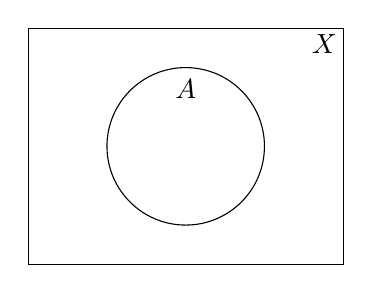
\begin{tikzpicture}

    % 画一个矩形
    \draw[thin] (0,0) rectangle (4,3);

    % 画一个圆形
    \draw[thin] (2,1.5) circle (1);

    % 插入文字
    \node[anchor=north, inner sep=4pt] at (2,2.5) {$A$};
    \node[anchor=north east, inner sep=2pt] at (4,3) {$X$};

  \end{tikzpicture}
\end{figure}

我们可以用维恩图来表示两个集合 $A, B$ 之间三种可能的关系如下。

\begin{figure}[H]
  \centering
  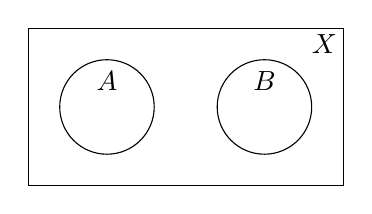
\begin{tikzpicture}

    % 画一个矩形
    \draw[thin] (0,0) rectangle (4,2);

    % 画一个圆形
    \draw[thin] (1,1) circle (0.6);
    \draw[thin] (3,1) circle (0.6);

    % 插入文字
    \node[anchor=north, inner sep=4pt] at (1,1.6) {$A$};
    \node[anchor=north, inner sep=4pt] at (3,1.6) {$B$};
    \node[anchor=north east, inner sep=2pt] at (4,2) {$X$};

  \end{tikzpicture}
  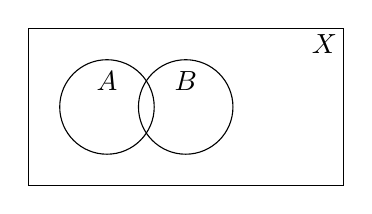
\begin{tikzpicture}

    % 画一个矩形
    \draw[thin] (0,0) rectangle (4,2);

    % 画一个圆形
    \draw[thin] (1,1) circle (0.6);
    \draw[thin] (2,1) circle (0.6);

    % 插入文字
    \node[anchor=north, inner sep=4pt] at (1,1.6) {$A$};
    \node[anchor=north, inner sep=4pt] at (2,1.6) {$B$};
    \node[anchor=north east, inner sep=2pt] at (4,2) {$X$};

  \end{tikzpicture}
  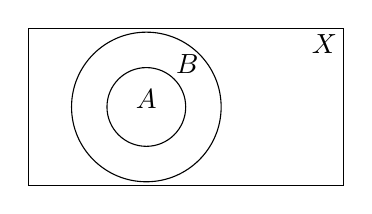
\begin{tikzpicture}

    % 画一个矩形
    \draw[thin] (0,0) rectangle (4,2);

    % 画一个圆形
    \draw[thin] (1.5,1) circle (0.5);
    \draw[thin] (1.5,1) circle (0.95);

    % 插入文字
    \node[anchor=north east, inner sep=2pt] at (2.24,1.74) {$B$};
    \node[anchor=north, inner sep=2pt] at (1.5,1.3) {$A$};
    \node[anchor=north east, inner sep=2pt] at (4,2) {$X$};

  \end{tikzpicture}
\end{figure}%
最左边图示表示的是 $A, B$ 没有共同的元素，中间图示表示的是 $A, B$ 有共同元素但互相没有包含关系，而最右边表示的是 $A \subseteq B$。

有时维恩图可以帮助我们了解一些集合的性质，甚至给我们证明这些性质的提示。例如以下的图示便可以帮助我们理解命题 3.1.4 (2) “若 $A \subseteq B$ 且 $B \subseteq C$，则 $A \subseteq C$” 这个性质。
\begin{figure}[H]
  \centering
  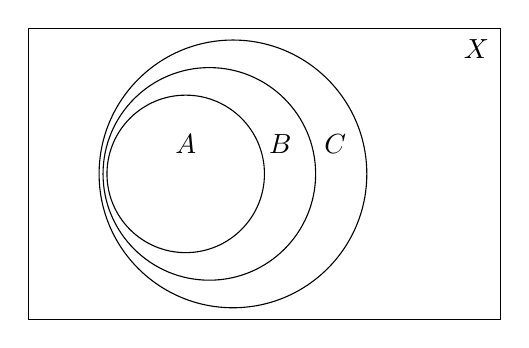
\begin{tikzpicture}

    % 画一个矩形
    \draw[thin] (0,0) rectangle (6,3.7);

    % 画一个圆形
    \draw[thin] (2,1.85) circle (1);
    \draw[thin] (2.3,1.85) circle (1.35);
    \draw[thin] (2.6,1.85) circle (1.7);

    % 插入文字
    \node[anchor=north, inner sep=4pt] at (2,2.5) {$A$};
    \node[anchor=north, inner sep=4pt] at (3.2,2.5) {$B$};
    \node[anchor=north, inner sep=4pt] at (3.9,2.5) {$C$};
    \node[anchor=north east, inner sep=4pt] at (6,3.7) {$X$};

  \end{tikzpicture}
\end{figure}

当然了维恩图只是让我们参考用，绝不能只是画个图就以为证明完成。

\begin{question}
假设 $A, B, C$ 为集合。已知 $A \subseteq B$。若 $B$ 和 $C$ 没有共同的元素，画出可能的维恩图。是否可以确定 $A$ 和 $C$ 没有共同元素？又若 $B$ 和 $C$ 有共同的元素，画出可能的维恩图，是否可确定 $A$ 和 $C$ 有共同元素？同样地，分 $A, C$ 有/没有共同元素的情况，画出可能的维恩图，并探讨是否依此可确定 $B, C$ 有没有共同元素。
\end{question}

最后提醒大家千万不要把 “$\in$”（属于）和 “$\subseteq$”（包含于）弄混淆。“$\in$” 指的是元素和集合之间的关系，而 “$\subseteq$” 指的是两集合间的关系。对于集合我们有 $A \subseteq B$ 且 $B \subseteq C$ 则 $A \subseteq C$ 的性质，但对于元素 $A \in B$ 且 $B \in C$ 未必可得 $A \in C$。例如 $A = \{1\}$, $B = \{\{1\}\}$, $C = \{\{\{1\}\}\}$。我们有 $A \in B$ 且 $B \in C$，但很明显地 $A \notin C$。

\section{集合运算}

所谓集合运算（set operation），\index{集合运算（set operation）}就是利用两个已知的集合得到另一个集合的方法。我们将介绍集合间几种重要的运算，即交集、并集和差集，并探讨这几种集合运算之间重要的性质。

\subsection{交集与并集}

首先我们定义交集与并集。

\begin{definition}
设 $A, B$ 为集合。我们令 $A \cap B = \{x : x \in A \text{ 且 }~ x \in B\}$ 称之为 $A$ 和 $B$ 的{\bf 交集（intersection）}。\index{交集（intersection）}令 $A \cup B = \{x : x \in A \text{ 或 }~ x \in B\}$ 称之为 $A$ 和 $B$ 的{\bf 并集（union）}\index{并集（union）}。
\end{definition}

简单地说 $A \cap B$ 就是将 $A, B$ 共同的元素收集起来所得的集合，而 $A \cup B$ 是将 $A, B$ 所有的元素收集起来而得的集合。例如以下的例子。

\begin{example}
令 $A = \{1, 2, 3\}$, $B = \{2, 4, 6\}$。由于只有 $2$ 是同时属于 $A$ 且属于 $B$，所以得 $A \cap B = \{2\}$。而 $1, 3$ 虽没有在 $B$ 但都属于 $A$，符合属于 $A$ 或属于 $B$ 的条件，故知 $1, 3$ 皆属于 $A \cup B$。同理 $4, 6$ 亦属于 $A \cup B$。至于 $2$，既然同时属于 $A$ 和 $B$，当然符合属于 $A$ 或属于 $B$ 的条件，故知 $2$ 也属于 $A \cup B$。又由于没有其他的数在 $A$ 中或 $B$ 中，我们可以确定 $A \cup B = \{1, 2, 3, 4, 6\}$。
\end{example}

并集和交集与原来的集合是有关系的。例如在上面的例子中我们有 $A \cap B = \{2\} \subseteq A = \{1, 2, 3\}$ 以及 $B = \{2, 4, 6\} \subseteq A \cup B = \{1, 2, 3, 4, 6\}$。事实上，若 $x \in A \cap B$，表示 $x \in A$ 且 $x \in B$，故知 $x$ 一定属于 $A$ 且 $x$ 一定属于 $B$，所以我们有
\begin{equation}
(A \cap B) \subseteq A \quad \text{和} \quad (A \cap B) \subseteq B.
\end{equation}
注意 $A \cap B$ 有可能是空集，此时我们称 $A, B$ 为\textbf{不相交（disjoint）}。\index{不相交（disjoint）}不过空集包含于任意的集合，所以当 $A, B$ 为不相交时上式仍然成立。另一方面若 $x \in A$，则 $x$ 必属于 $A$ 或 $B$，所以 $x \in A \cup B$ 成立。我们有
\begin{equation}
A \subseteq (A \cup B) \quad \text{和} \quad B \subseteq (A \cup B).
\end{equation}

\begin{question}
试证明 $(A \cap A) = A$ 以及 $(A \cup A) = A$。
\end{question}

交集和并集在某种程度上可以说是保持包含关系的，事实上我们有以下的性质。

\begin{proposition}
设 $A, B, C, D$ 皆为集合，满足 $A \subseteq B$ 且 $C \subseteq D$。则
$$ (A \cap C) \subseteq (B \cap D) \quad \text{和} \quad (A \cup C) \subseteq (B \cup D). $$
\end{proposition}

\begin{proof}
因 $A \subseteq B$，可由 $x \in A$ 得 $x \in B$。同理因 $C \subseteq D$，可由 $x \in C$ 得 $x \in D$。现若 $x \in A \cap C$，表示 $x \in A$ 且 $x \in C$，故可得 $x \in B$ 且 $x \in D$。得证 $(A \cap C) \subseteq (B \cap D)$。同理，若 $x \in A \cup C$，表示 $x \in A$ 或 $x \in C$。当 $x \in A$ 时可得 $x \in B$，而当 $x \in C$ 时可得 $x \in D$。故由 $x \in A \cup C$ 可得 $x \in B \cup D$。得证 $(A \cup C) \subseteq (B \cup D)$。
\end{proof}

特别地，当 $A \subseteq B$ 且 $A \subseteq D$ 时，我们可以考虑 $C = A$ 的情形套用命题 3.2.3 得 $(A \cap A) \subseteq (B \cap D)$。又由于 $(A \cap A) = A$，得知 $A \subseteq (B \cap D)$。同理，当 $A \subseteq B$ 且 $C \subseteq B$ 时，我们有 $(A \cup C) \subseteq (B \cup B)$。又由于 $(B \cup B) = B$，得知 $(A \cup C) \subseteq B$。我们证得以下性质。既然这个结果是由命题 3.2.3 简单推导而得，我们就用推论 （corollary）称之。

\begin{corollary}
假设 $A, B, C, D, E$ 为集合。
\begin{enumerate}
  \item 若 $A \subseteq B$ 且 $A \subseteq C$，则 $A \subseteq (B \cap C)$。
  \item 若 $D \subseteq A$ 且 $E \subseteq A$，则 $(D \cup E) \subseteq A$。
\end{enumerate}
\end{corollary}

\begin{question}
试直接证明推论 3.2.4，并用此结果推导出命题 3.2.3。
\end{question}

我们也可利用交集或并集来判断两集合的包含关系。我们有以下的结果。

\begin{proposition}
假设 $A, B$ 为集合。则以下是等价的。
\begin{enumerate}[label={(\arabic*)}]
  \item $A \subseteq B$。
  \item $(A \cap B) = A$。
  \item $(A \cup B) = B$。
\end{enumerate}
\end{proposition}

\begin{proof}
我们证明 (1) $\Leftrightarrow$ (2) 以及 (1) $\Leftrightarrow$ (3)。

(1) $\Leftrightarrow$ (2)：假设 $A \subseteq B$，我们要证明 $(A \cap B) = A$。事实上由式子 (3.1) 我们知 $(A \cap B) \subseteq A$，故仅要证明 $A \subseteq (A \cap B)$。然而已知 $A \subseteq A$ 以及 $A \subseteq B$，故由推论 3.2.4 得 $A \subseteq (A \cap B)$。因此证明了 (1) $\Rightarrow$ (2)。另一方面，由式子 (3.1) 我们知 $(A \cap B) \subseteq B$。故由 $A = (A \cap B)$ 可得 $A \subseteq B$，证明了 (2) $\Rightarrow$ (1)。

(1) $\Leftrightarrow$ (3)：假设 $A \subseteq B$，我们要证明 $(A \cup B) = B$。事实上由式子 (3.2) 我们知 $B \subseteq (A \cup B)$，故仅要证明 $(A \cup B) \subseteq B$。然而已知 $A \subseteq B$ 以及 $B \subseteq B$，故由推论 3.2.4，得 $(A \cup B) \subseteq B$。因此证明了 (1) $\Rightarrow$ (3)。另一方面，由式子 (3.2) 我们知 $A \subseteq (A \cup B)$。故由 $(A \cup B) = B$ 可得 $A \subseteq B$，证明了 (3) $\Rightarrow$ (1)。
\end{proof}

由定义我们知道 “交集” 和逻辑的 “且” 有关，而 “并集” 和 “或” 有关。所以我们很容易推得以下的关系：
\begin{enumerate}[label={(\arabic*)}]
  \item $A \cap B = B \cap A$。
  \item $A \cup B = B \cup A$。
  \item $(A \cap B) \cap C = A \cap (B \cap C)$。
  \item $(A \cup B) \cup C = A \cup (B \cup C)$。
\end{enumerate}
由于 (3) 的关系，以后多个集合的交集我们便省略括弧不必去强调哪几个先作交集，例如直接写成 $A \cap B \cap C$。同理由于 (4)，以后多个集合的并集我们也省略括弧，例如直接写成 $A \cup B \cup C$。

利用逻辑 $\wedge, \vee$ 之间的分配性质，即
$$ ((P \wedge Q) \vee R) \sim ((P \vee R) \wedge (Q \vee R)), $$
$$ ((P \vee Q) \wedge R) \sim ((P \wedge R) \vee (Q \wedge R)), $$
我们有以下的性质。

\begin{proposition}
假设 $A, B, C$ 为集合，则
$$ ((A \cap B) \cup C) = (A \cup C) \cap (B \cup C), $$
$$ ((A \cup B) \cap C) = (A \cap C) \cup (B \cap C). $$
\end{proposition}

\begin{proof}
首先由 $(A \cap B) \subseteq A$ 以及 $C \subseteq C$ 利用命题 3.2.3 得 $((A \cap B) \cup C) \subseteq (A \cup C)$。同理知 $((A \cap B) \cup C) \subseteq (B \cup C)$。再利用推论 3.2.4 得 $((A \cap B) \cup C) \subseteq (A \cup C) \cap (B \cup C)$。另一方面假设 $x \in (A \cup C) \cap (B \cup C)$ 表示 $x \in A \cup C$ 且 $x \in B \cup C$。我们利用分类讨论，考虑 $x \in C$ 和 $x \notin C$ 这两种情况。若 $x \in C$，则当然 $x \in (A \cap B) \cup C$。而若 $x \notin C$，则由 $x \in A \cup C$ 且 $x \in B \cup C$，知 $x \in A$ 且 $x \in B$，亦即 $x \in A \cap B$。故此时仍有 $x \in (A \cap B) \cup C$。也就是说不管哪种情况，我们都可以由 $x \in (A \cup C) \cap (B \cup C)$ 推得 $x \in (A \cap B) \cup C$，得证 $((A \cup C) \cap (B \cup C)) \subseteq (A \cap B) \cup C$。故知 $((A \cap B) \cup C) = (A \cup C) \cap (B \cup C)$。

至于 $((A \cup B) \cap C) = (A \cap C) \cup (B \cap C)$ 的证明，首先由 $A \subseteq (A \cup B)$ 以及 $C \subseteq C$ 利用命题 3.2.3 得 $(A \cap C) \subseteq ((A \cup B) \cap C)$，同理我们有 $(B \cap C) \subseteq ((A \cup B) \cap C)$。故由推论 3.2.4 知 $(A \cap C) \cup (B \cap C) \subseteq ((A \cup B) \cap C)$。另一方面，若 $x \in (A \cup B) \cap C$，表示 $x \in A \cup B$ 且 $x \in C$。由 $x \in A \cup B$，我们知 $x \in A$ 或 $x \in B$。当 $x \in A$ 时，由于已知 $x \in C$，故得 $x \in A \cap C$。此时自然有 $x \in (A \cap C) \cup (B \cap C)$。同理，当 $x \in B$ 时，可得 $x \in B \cap C$。因此也有 $x \in (A \cap C) \cup (B \cap C)$，得证 $((A \cup B) \cap C) \subseteq (A \cap C) \cup (B \cap C)$。故知 $((A \cup B) \cap C) = (A \cap C) \cup (B \cap C)$。
\end{proof}

\begin{question}
试利用命题 3.2.5 中 (1) $\Rightarrow$ (2) 的结果以及命题 3.2.6 证明命题 3.2.5 中 (2) $\Rightarrow$ (3)。
\end{question}

\subsection{差集}

我们定义何谓差集。

\begin{definition}
假设 $A, B$ 为集合，定义 $A \setminus B = \{x : x \in A \text{ 且 }~ x \notin B\}$，称之为 $B$ 在 $A$ 中的{\bf 差集（set difference）}。\index{差集（set difference）}若 $X$ 为全集，则令 $A^c = X \setminus A = \{x : x \notin A\}$ 称之为 $A$ 的{\bf 补集（complement）}\index{补集（complement）}。
\end{definition}

注意 $A^c$ 的定义原本应为 $\{x : x \in X \text{ 且 }~ x \notin A\}$，但因 $X$ 为全集，我们知道所有元素皆在 $X$ 中，故省略 $x \in X$ 直接写 $x \notin A$。所以在使用补集时要特别注意是否已明确说明了什么是全集，否则会有符号不唯一的问题。例如若 $\mathbb{Q}$ 为全集，则 $\mathbb{Q}^c = \emptyset$，而当全集为 $\mathbb{R}$ 时，$\mathbb{Q}^c$ 就是所有无理数所成的集合了。

利用补集的符号，依定义我们有 $A \setminus B = A \cap B^c$，从这里我们知道一般情况下 $A \setminus B$ 和 $B \setminus A$ 是不相同的。事实上我们有 $(A \setminus B) \cap (B \setminus A) = \emptyset$。这是因为很明显地 $A \cap A^c = \emptyset$ 且 $B \cap B^c = \emptyset$，故知
$$ (A \setminus B) \cap (B \setminus A) = (A \cap B^c) \cap (B \cap A^c) = (A \cap A^c) \cap (B \cap B^c) = \emptyset. $$

\begin{example}
假设 $X = \{1, 2, 3, 4, 5, 6\}$, $A = \{1, 2, 3\}$, $B = \{2, 4, 6\}$。因 $1, 3 \in A$ 且 $1 \notin B$ 且 $3 \notin B$，知 $1, 3 \in A \setminus B$。虽然 $2 \in A$ 但是 $2 \in B$，故 $2 \notin A \setminus B$。得 $A \setminus B = \{1, 3\}$。同理可得 $B \setminus A = \{4, 6\}$。我们有 $(A \setminus B) \cap (B \setminus A) = \{1, 3\} \cap \{4, 6\} = \emptyset$。又 $1, 3, 5 \in X$ 且 $1, 3, 5$ 皆不在 $B$ 中，故知 $1, 3, 5 \in B^c$。而 $2, 4, 6 \in B$ 故 $2, 4, 6$ 皆不属于 $B^c$，得 $B^c = \{1, 3, 5\}$。最后考虑 $A \cap B^c$ 得 $A \cap B^c = \{1, 2, 3\} \cap \{1, 3, 5\} = \{1, 3\} = A \setminus B$。
\end{example}

接下来我们看差集的一些性质，其实这些性质我们可以用元素的方式证明，不过在证明时由于常出现否定的问题所以经常要用反证法，如此反反复复，容易搞混。但如使用补集符号，就可以化繁为简。所以我们先介绍有关于补集的一些性质，再处理差集的问题。

\begin{proposition}
假设 $A, B$ 为集合，我们有以下的性质。
\begin{enumerate}[label={(\arabic*)}]
  \item $(A^c)^c = A$。
  \item $(A \cap B)^c = (A^c \cup B^c)$。
  \item $(A \cup B)^c = (A^c \cap B^c)$。
  \item $A \subseteq B$ 当且仅当 $B^c \subseteq A^c$。
\end{enumerate}
\end{proposition}

\begin{proof}
这些性质都可以利用前面逻辑相关的等价推导。我们主要使用的方式就是 $x \notin A$ 是 $x \in A$ 的否定，所以
$$ (x \in A^c) \sim (x \notin A)\sim \neg(x \in A). $$

(1) $x \in (A^c)^c$ 表示 $x \notin A^c$，即 $\neg(x \in A^c)$。等同于 $\neg(x \notin A)$，亦即 $\neg(\neg(x \in A))$。因此由式子(1.7)知此与 $x \in A$ 等价，故得证。

(2) $x \in (A \cap B)^c \sim \neg(x \in (A \cap B)) \sim \neg((x \in A) \wedge (x \in B))$。由式子(1.8)知此与 $\neg(x \in A) \vee \neg(x \in B)$ 等价，亦即 $(x \in A^c) \vee (x \in B^c)$，故得证等同于 $x \in (A^c \cup B^c)$。

(3) $x \in (A \cup B)^c \sim \neg(x \in (A \cup B)) \sim \neg((x \in A) \vee (x \in B))$。由式子(1.9)知此与 $\neg(x \in A) \wedge \neg(x \in B)$ 等价，亦即 $(x \in A^c) \wedge (x \in B^c)$，故得证等同于 $x \in (A^c \cap B^c)$。

(4) 由于 $A \subseteq B$ 等价于 $(x \in A) \Rightarrow (x \in B)$，且 $B^c \subseteq A^c$ 等价于 $\neg(x \in B) \Rightarrow \neg(x \in A)$。由式子(1.11)我们有$((x \in A) \Rightarrow (x \in B)) \sim (\neg(x \in B) \Rightarrow \neg(x \in A))$，故得证。
\end{proof}

利用命题 3.2.9，我们立即可得以下的定理。

\begin{corollary}
假设 $A, B, C$ 为集合，我们有以下的性质。
\begin{enumerate}[label={(\arabic*)}]
  \item $(C \setminus (C \setminus A)) = (C \cap A)$。
  \item $C \setminus (A \cap B) = (C \setminus A) \cup (C \setminus B)$。
  \item $C \setminus (A \cup B) = (C \setminus A) \cap (C \setminus B)$。
  \item 若 $A \subseteq B$ 则 $(C \setminus B) \subseteq (C \setminus A)$。
\end{enumerate}
\end{corollary}

\begin{proof}
我们使用补集、交集、并集之间的关系证明。

(1) 依定义 $(C \setminus (C \setminus A)) = C \cap (C \setminus A)^c = C \cap (C \cap A^c)^c$。由命题 3.2.9 (1)(2)，$(C \cap A^c)^c = C^c \cup (A^c)^c = C^c \cup A$，故得 $(C \setminus (C \setminus A)) = C \cap (C^c \cup A)$。再由分配律
$$ C \cap (C^c \cup A) = (C \cap C^c) \cup (C \cap A) = \emptyset \cup (C \cap A) $$
得证 $(C \setminus (C \setminus A)) = (C \cap A)$。

(2) 依定义 $C \setminus (A \cap B) = C \cap (A \cap B)^c$。由命题 3.2.9 (2)，$(A \cap B)^c = (A^c \cup B^c)$，故得 $C \setminus (A \cap B) = C \cap (A^c \cup B^c)$。再由分配律 $C \cap (A^c \cup B^c) = (C \cap A^c) \cup (C \cap B^c)$。得证 $C \setminus (A \cap B) = (C \setminus A) \cup (C \setminus B)$。

(3) 依定义 $C \setminus (A \cup B) = C \cap (A \cup B)^c$。由命题 3.2.9 (3)，$(A \cup B)^c = (A^c \cap B^c)$，故得 $C \setminus (A \cup B) = C \cap (A^c \cap B^c)$。再由 $C \cap (A^c \cap B^c) = (C \cap A^c) \cap (C \cap B^c)$。得证 $C \setminus (A \cup B) = (C \setminus A) \cap (C \setminus B)$。

(4) 依定义 $C \setminus B = C \cap B^c$。现若 $A \subseteq B$ 由命题 3.2.9 (4) 可得 $B^c \subseteq A^c$，故得 $C \cap B^c \subseteq C \cap A^c$，得证 $(C \setminus B) \subseteq (C \setminus A)$。
\end{proof}

推论 3.2.10 (4) 的反向是不正确的，不过我们有以下之结果。

\begin{proposition}
假设 $A, B, C$ 为集合。$(C \cap A) \subseteq (C \cap B)$ 当且仅当 $(C \setminus B) \subseteq (C \setminus A)$。
特别地，若已知 $A \subseteq C$，则 $A \subseteq B$ 当且仅当 $(C \setminus B) \subseteq (C \setminus A)$。
\end{proposition}

\begin{proof}
首先注意 $C \setminus A = C \setminus (C \cap A)$，这是因为由推论 3.2.10 (2)，
$$ C \setminus (C \cap A) = (C \setminus C) \cup (C \setminus A) = \emptyset \cup (C \setminus A) = C \setminus A. $$
同理 $C \setminus B = C \setminus (C \cap B)$。

现若 $(C \cap A) \subseteq (C \cap B)$，利用推论 3.2.10 (4) 可得 $C \setminus (C \cap B) \subseteq C \setminus (C \cap A)$，得证 $(C \setminus B) \subseteq (C \setminus A)$。反之，若 $(C \setminus B) \subseteq (C \setminus A)$，则同样由推论 3.2.10 (4) 得 $C \setminus (C \setminus A) \subseteq C \setminus (C \setminus B)$。再由命题 3.2.10 (1) 得证 $(C \cap A) \subseteq (C \cap B)$。

由推论 3.2.10 (4) 已知若 $A \subseteq B$ 则 $(C \setminus B) \subseteq (C \setminus A)$。故当已知 $A \subseteq C$，我们仅要证明：若 $(C \setminus B) \subseteq (C \setminus A)$ 则 $A \subseteq B$。此时由前知 $(C \setminus B) \subseteq (C \setminus A)$ 可得 $(C \cap A) \subseteq (C \cap B)$。故由 $A \subseteq C$ 的假设得 $A = (C \cap A) \subseteq (C \cap B)$。但 $(C \cap B) \subseteq B$，故得证 $A \subseteq B$。
\end{proof}

\begin{question}
$C \setminus (B \setminus A)$ 会等于 $(C \setminus B) \setminus A$ 吗？试证明 $C \setminus (B \setminus A) = (C \setminus B) \cup (C \cap A)$ 以及 $(C \setminus B) \setminus A = C \setminus (B \cup A)$。
\end{question}

其实这些集合运算之间的关系与性质，都可以直接各边取一元素，利用第一章所介绍逻辑联结词的性质得到集合包含关系，最后证得两边集合相等。另一方面我们也可套用这一章中所介绍各集合的运算的性质推导。这两者方法并无好坏之分，虽然有时直接套用集合运算的性质推导很快速，但它并非万能。在这里我们并不是鼓励大家用背诵的方式记忆这么多的性质，而是希望大家能够学习如何利用一些已知的性质推导出新的定理。最后我们再看一个例子。

\begin{example}
假设 $A, B, C$ 为集合且 $B^c \subseteq A$，我们要证明 $((C \setminus A) \cup B) = B$。
\end{example}

方法一：我们用元素的方法处理。首先已知 $B \subseteq ((C \setminus A) \cup B)$，故要证明等式成立只要证明 $((C \setminus A) \cup B) \subseteq B$。现假设 $x \in ((C \setminus A) \cup B)$，我们要证明 $x \in B$。然而 $x \in ((C \setminus A) \cup B)$ 表示 $x \in C \setminus A$ 或 $x \in B$。如果 $x \in B$，则证明结束，所以我们仅要讨论 $x \in C \setminus A$ 的情形，即 $x \in C$ 且 $x \notin A$。因为无法直接证明 $x \in B$，所以我们可以考虑反证法，即假设 $x \notin B$ 而得到矛盾。现若 $x \notin B$，表示 $x \in B^c$，故由 $B^c \subseteq A$ 的假设得 $x \in A$。此与 $x \notin A$ 相矛盾，故知 $x \in B$。得证 $((C \setminus A) \cup B) \subseteq B$。

方法二：我们也可完全用前面证得的性质处理。首先看到等式左右两边都有 $B$，所以我们可以利用命题 3.2.5。也就是说若能证明 $(C \setminus A) \subseteq B$，则可得证 $((C \setminus A) \cup B) = B$。如何证明 $(C \setminus A) \subseteq B$ 呢？由于 $(C \setminus A) \subseteq C$，利用命题 3.2.11，我们只要验证 $(C \setminus B) \subseteq (C \setminus (C \setminus A))$。然而左边 $C \setminus B = C \cap B^c$，右边 $C \setminus (C \setminus A) = C \cap A$，所以由 $B^c \subseteq A$ 得证 $(C \setminus B) \subseteq (C \setminus (C \setminus A))$，因而得 $(C \setminus A) \subseteq B$。

\section{加标集族}

在前一节中，我们谈交集或并集时，是将其视为两个集合间的运算。不过当我们知道交集和并集有所谓的结合律后，我们便可以谈论多个集合的并集与交集了。这一节中，我们藉由适当的符号与定义的推广，将探讨任意多个集合的并集与交集问题。大致上之前谈的两个集合的交集与并集的性质，都可以推广到更一般的情形。不过处理无限多个集合的情况，有些地方可能和有限的情况稍有不同，要特别留意。

当我们谈论有限多个集合的交集和并集时，如果集合个数不多，例如 5 个集合 $A, B, C, D, E$ 的交集，我们直接用 $A \cap B \cap C \cap D \cap E$ 来表示。这里我们都可以不用括弧区分到底哪两个集合先交集后再和其他的集合做交集，因为交集有结合律。我们也不必担心交集的顺序，因为交集有交换性。同样地对于并集也是如此。当集合的个数太多时，像前面这样一一列出就不切实际了。遇到这种情形，我们可以把要处理的集合一一编号，例如有 100 个集合，我们就编成 $A_1, A_2, \dots, A_{100}$（当然了，这些 $A_i$ 是什么应说明清楚）。然后这些集合的交集与并集我们便像处理加法的求和（summation）符号，将这些集合的交集与并集分别用 $\bigcap_{i=1}^{100} A_i$，$\bigcup_{i=1}^{100} A_i$ 来表示。例如若 $A_i = [i-1, i]$（即介于 $i-1$ 和 $i$ 之间的实数），则 $\bigcap_{i=1}^{100} A_i = \emptyset$，$\bigcup_{i=1}^{100} A_i = [0, 100]$。

如果有无穷多集合怎么办？像前面的例子，如果对所有的自然数 $i \in \mathbb{N}$，$A_i$ 皆有定义，我们可以考虑对所有的 $A_i$ 的交集和并集。这时候我们一般可以学无穷级数的方法，将这些交集和并集分别表示成 $\bigcap_{i=1}^{\infty} A_i$，$\bigcup_{i=1}^{\infty} A_i$。当然了，这样的符号底下表示的是 $i$ 从哪一个数开始，上面表示的是到哪一个为止，所以我们要考虑 $A_5, A_6, A_7, A_8$ 的交集和并集就可以分别用 $\bigcap_{i=5}^{8} A_i$，$\bigcup_{i=5}^{8} A_i$ 来表示。因此一般若要谈 $i$ 从 $m$ 到 $n$ 的 $A_i$ 之交集与并集，我们便分别用 $\bigcap_{i=m}^{n} A_i$，$\bigcup_{i=m}^{n} A_i$ 来表示。而要表达所有 $i$ 大于等于 $m$ 的 $A_i$ 之交集与并集，我们便分别用 $\bigcap_{i=m}^{\infty} A_i$，$\bigcup_{i=m}^{\infty} A_i$ 来表示。这里要注意，很多同学会误以为 $\bigcap_{i=m}^{\infty} A_i$，$\bigcup_{i=m}^{\infty} A_i$ 是 $\bigcap_{i=m}^{n} A_i$，$\bigcup_{i=m}^{n} A_i$ 当 $n$ 趋近于 $\infty$ 的极限。这个说法是有问题的，因为我们从未定义过 “集合的极限”。

不过这些符号仍不够我们的需求。有时我们要探讨的集合，它们的个数是不能像整数一样一个一个数的。例如实数，就无法一个一个数。所以若我们谈的集合和实数有关，如 $(-r, r)$ 其中 $r > 0$这样的区间，要如何表达所有这样的区间的交集与并集呢？于是乎，我们引进了\textbf{指标集（index set）}\index{指标集（index set）}的概念。所谓指标集就是你要用来 “编码” 的东西所成的集合。例如前面 $A_i = [i-1, i]$ 的例子，我们考虑的 $i$ 是所有的自然数 $\mathbb{N}$，所以此时 $\mathbb{N}$ 便是我们的指标集。而若要探讨 $[-r, r]$ 的情形，我们可以用正实数 $\mathbb{R}^+$ 为我们的指标集，将要考虑的区间编码成 $A_r = [-r, r]$。这样将所有被编码好的集合 $A_r, r \in \mathbb{R}^+$ 收集在一起，便是所谓的\textbf{加标集族（indexed family）}\index{加标集族（indexed family）}了。所以一般来说，我们要先说好指标集是什么集合，接下来要说明要探讨的集合如何用指标集里的元素编码，这样才能形成一个加标集族。也就是说若 $I$ 为指标集，我们必须说明 $A_i$ 是什么，这样 $\{A_i, i \in I\}$ 便会是一个加标集族。

接下来，我们便是要定义一个加标集族里的集合的交集与并集。注意，即使只有有限个集合，我们仍可将其视为加标集族。例如两个集合 $A, B$，我们仍可将其视为指标集为 $I = \{1, 2\}$ 的加标集族，其中 $A_1 = A, A_2 = B$。所以我们定义加标集族的交集与并集需与有限集合的交集与并集一致。当我们有两个集合 $A, B$ 时，要求交集的元素必须在每一个集合中；而并集里的元素需在 $A, B$ 某一个中。所以我们有以下的定义。

\begin{definition}
假设 $I$ 为指标集，而 $\{A_i, i \in I\}$ 为以 $I$ 为指标集的加标集族。
定义此加标集族的交集\index{交集（intersection）!加标集族的$\sim$（of indexed family）}为
$$ \bigcap_{i \in I} A_i = \{x : x \in A_i, \forall i \in I\}. $$
定义此加标集族的并集\index{并集（union）!加标集族的$\sim$（of indexed family）}为
$$ \bigcup_{i \in I} A_i = \{x : x \in A_i, \exists i \in I\}. $$
\end{definition}

利用此定义，我们看以下的例子。

\begin{example}
考虑指标集 $I$ 为大于 $1$ 的整数。对任意 $i \in I$，令 $A_i = \{m/i : m \in \mathbb{Z}\}$。我们要证明
$$ \bigcap_{i \in I} A_i = \mathbb{Z}, \quad \bigcup_{i \in I} A_i = \mathbb{Q}. $$
\end{example}
首先，任意 $n \in \mathbb{Z}$，我们都可以写成 $n = ni/i$。由于 $ni \in \mathbb{Z}$，故得 $n \in A_i, \forall i \in I$。得证 $\mathbb{Z} \subseteq \bigcap_{i \in I} A_i$。另一方面，若 $x \in \bigcap_{i \in I} A_i$，表示对任意 $i \in I$ 皆有 $x \in A_i$。现由于 $x \in A_2$ 以及 $x \in A_3$，我们有 $x = m/2$ 且 $x = m'/3$，其中 $m, m' \in \mathbb{Z}$。然而此即表示 $3m = 2m'$，故知 $3m$ 必为偶数。因而得知 $m$ 为偶数 $2n$，其中 $n \in \mathbb{Z}$。代回得 $x = m/2 = n \in \mathbb{Z}$。得证 $\bigcap_{i \in I} A_i \subseteq \mathbb{Z}$，故 $\bigcap_{i \in I} A_i = \mathbb{Z}$。

现若 $x \in \mathbb{Q}$，依有理数之定义，$x$ 可写成 $m/n$，其中 $m \in \mathbb{Z}, n \in \mathbb{N}$。现若 $n = 1$，即 $x = m \in \mathbb{Z}$。我们可以将 $x$ 写成 $x = 2m/2$，知此时 $x \in A_2$。而若 $n \geq 2$，表示 $n \in I$，故此时 $x \in A_n$。得证 $\mathbb{Q} \subseteq \bigcup_{i \in I} A_i$。另一方面，若 $x \in \bigcup_{i \in I} A_i$，表示存在 $n \in I$，使得 $x \in A_n$。故依定义得 $x = m/n$，其中 $m \in \mathbb{Z}$。此即表示 $x \in \mathbb{Q}$，得证 $\bigcup_{i \in I} A_i \subseteq \mathbb{Q}$，故 $\bigcup_{i \in I} A_i = \mathbb{Q}$。

\begin{question}
令 $A_i$ 如例 3.3.2 所设。利用当 $m \in \mathbb{Z}$ 时，若 $p, q$ 为两互质整数且 $p$ 整除 $mq$，则 $p$ 整除 $m$ 之事实，证明若 $p, q$ 为两互质整数，则 $A_p \cap A_q = \mathbb{Z}$。依此证明当 $m \in \mathbb{N}$，$\bigcap_{i=m}^{\infty} A_i = \mathbb{Z}$。
\end{question}

现在我们探讨一些有关两集合的交集与并集的性质，是否可以推广到更一般加标集族的情形。首先命题 3.2.3 是可以推广的。

\begin{proposition}
假设 $\{A_i, i \in I\}$, $\{B_i, i \in I\}$ 是以 $I$ 为指标集的两组加标集族。若对于所有 $i \in I$ 皆有 $A_i \subseteq B_i$，则
$$ \bigcap_{i \in I} A_i \subseteq \bigcap_{i \in I} B_i \quad \text{且} \quad \bigcup_{i \in I} A_i \subseteq \bigcup_{i \in I} B_i. $$
\end{proposition}

\begin{proof}
设 $x \in \bigcap_{i \in I} A_i$，表示对所有 $i \in I$，皆有 $x \in A_i$，故由 $A_i \subseteq B_i$，得 $x \in B_i$。因为这是对任意的 $i \in I$ 皆成立，故得 $x \in \bigcap_{i \in I} B_i$。得证 $\bigcap_{i \in I} A_i \subseteq \bigcap_{i \in I} B_i$。

现若 $x \in \bigcup_{i \in I} A_i$，表示存在 $i \in I$ 使得 $x \in A_i$，故由 $A_i \subseteq B_i$，得 $x \in B_i$。此即表示 $x \in \bigcup_{i \in I} B_i$，得证 $\bigcup_{i \in I} A_i \subseteq \bigcup_{i \in I} B_i$。
\end{proof}

很容易知道，若对于任意 $i \in I$，皆有 $A_i = A$，则 $\bigcap_{i \in I} A_i = A$ 且 $\bigcup_{i \in I} A_i = A$。所以我们套用命题 3.3.3，有以下推论 3.2.4 的推广。

\begin{corollary}
假设 $A, B$ 为集合且 $\{A_i, i \in I\}$, $\{B_i, i \in I\}$ 是以 $I$ 为指标集的加标集族。
\begin{enumerate}
  \item 若对于所有 $i \in I$ 皆有 $A \subseteq A_i$，则 $A \subseteq \bigcap_{i \in I} A_i$。
  \item 若对于所有 $i \in I$ 皆有 $B_i \subseteq B$，则 $\bigcup_{i \in I} B_i \subseteq B$。
\end{enumerate}
\end{corollary}

虽然前面几个结果显示一些关于有限多个集合的交集或并集的性质可以推广到无穷多个集合的交集或并集，不过这并不是完全对的。例如有可能有一些集合当你在它们中任意取有限多个做交集时都不是空集，但是取无穷多个做交集时有可能会是空集。我们有以下的例子。

\begin{example}
我们要举例说明有可能一个以自然数 $\mathbb{N}$ 为指标集的加标集族 $\{A_i, i \in I\}$，满足对所有 $n \in \mathbb{N}$ 皆有 $\bigcap_{i=1}^{n} A_i$ 不是空集（甚至会有无穷多个元素），但 $\bigcap_{i=1}^{\infty} A_i$ 是空集。

事实上对所有 $i \in \mathbb{N}$ 考虑 $A_i$ 为开区间 $(i, \infty)$。此时 $A_i$ 满足 $A_i \neq \emptyset$ 且当 $j \geq i$ 时，$A_j \subseteq A_i$。因此得 $\bigcap_{i=1}^{n} A_i = A_n = (n, \infty) \neq \emptyset$。但 $\bigcap_{i=1}^{\infty} A_i = \emptyset$。这是因为若 $x \in \bigcap_{i=1}^{\infty} A_i$，则因 $x \in \mathbb{R}$ 必存在 $n \in \mathbb{N}$ 满足 $n > x$。我们得 $x \notin A_n = (n, \infty)$。此与 $x \in \bigcap_{i=1}^{\infty} A_i$ 相矛盾，得证 $\bigcap_{i=1}^{\infty} A_i = \emptyset$。
\end{example}

从上面这个例子我们知道，一些在有限多个集合的交集或并集会对的情形，在无穷多个集合的时候有可能是错的，所以还是要多加留意。

\begin{question}
假设 $A_i$ 为例 3.3.5 中的开区间 $(i, \infty)$，为何不是 $\bigcap_{i=1}^{\infty} A_i = \{\infty\}$？
\end{question}

关于交集与并集分配律的性质，我们有以下命题 3.2.6 的推广。

\begin{proposition}
假设 $B$ 为集合，且 $\{A_i, i \in I\}$ 是以 $I$ 为指标集的加标集族。则
$$ \left( \bigcap_{i \in I} A_i \right) \cup B = \bigcap_{i \in I} (A_i \cup B) \quad \text{且} \quad \left( \bigcup_{i \in I} A_i \right) \cap B = \bigcup_{i \in I} (A_i \cap B). $$
\end{proposition}

\begin{proof}
由于对所有 $k \in I$ 皆有 $(\bigcap_{i \in I} A_i) \subseteq (A_k \cup B)$ 且 $B \subseteq (A_k \cup B)$，由推论 3.2.4 (2) 知 $((\bigcap_{i \in I} A_i) \cup B) \subseteq (A_k \cup B)$。因为这是对任意 $k \in I$ 皆对，故由推论 3.3.4 (1) 知
$ \left( \left( \bigcap_{i \in I} A_i \right) \cup B \right) \subseteq \bigcap_{i \in I} (A_i \cup B). $

另一方面，若 $x \in \bigcap_{i \in I} (A_i \cup B)$，则对所有 $i \in I$，皆有 $x \in A_i$ 或 $x \in B$。我们分 $x \in B$ 以及 $x \notin B$ 两种情况来讨论。若 $x \in B$，则自然有 $x \in (\bigcap_{i \in I} A_i) \cup B$。而若 $x \notin B$，则知 $x \in A_i$ 且由于这是对所有 $i \in I$ 皆成立，故得 $x \in \bigcap_{i \in I} A_i$，因此 $x \in (\bigcap_{i \in I} A_i) \cup B$。得证 $\bigcap_{i \in I} (A_i \cup B) \subseteq ((\bigcap_{i \in I} A_i) \cup B)$，故 $(\bigcap_{i \in I} A_i) \cup B = \bigcap_{i \in I} (A_i \cup B)$。

同理，对所有 $k \in I$ 皆有 $(A_k \cap B) \subseteq (\bigcup_{i \in I} A_i)$ 且 $(A_k \cap B) \subseteq B$，由推论 3.2.4 (1) 知 $(A_k \cap B) \subseteq (\bigcup_{i \in I} A_i) \cap B$。因为这是对任意 $k \in I$ 皆对，故由推论 3.3.4 (2) 知
$ \bigcup_{i \in I} (A_i \cap B) \subseteq \left( \bigcup_{i \in I} A_i \right) \cap B. $

另一方面，若 $x \in (\bigcup_{i \in I} A_i) \cap B$，表示 $x \in \bigcup_{i \in I} A_i$ 且 $x \in B$。因此存在 $i \in I$，使得 $x \in A_i$ 且 $x \in B$。亦即存在 $i \in I$ 使得 $x \in A_i \cap B$。故知此时 $x \in \bigcup_{i \in I} (A_i \cap B)$，得证 $((\bigcup_{i \in I} A_i) \cap B) \subseteq \bigcup_{i \in I} (A_i \cap B)$，故 $(\bigcup_{i \in I} A_i) \cap B = \bigcup_{i \in I} (A_i \cap B)$。
\end{proof}

最后我们推广有限集合差集的德摩根定律\index{德摩根定律（DeMorgan's laws）}（命题 3.2.9 (2)(3)）。

\begin{proposition}
假设 $C$ 为集合且 $\{A_i, i \in I\}$ 是以 $I$ 为指标集的加标集族，我们有以下的性质。
\begin{enumerate}
  \item $C \setminus (\bigcap_{i \in I} A_i) = \bigcup_{i \in I} (C \setminus A_i)$。特别地，我们有 $(\bigcap_{i \in I} A_i)^c = \bigcup_{i \in I} A_i^c$。
  \item $C \setminus (\bigcup_{i \in I} A_i) = \bigcap_{i \in I} (C \setminus A_i)$。特别地，我们有 $(\bigcup_{i \in I} A_i)^c = \bigcap_{i \in I} A_i^c$。
\end{enumerate}
\end{proposition}

\begin{proof}
(1)：我们先证 $(\bigcap_{i \in I} A_i)^c = \bigcup_{i \in I} A_i^c$。为了方便我们直接用逻辑等价来证明。因 $x \in (\bigcap_{i \in I} A_i)^c$ 表示 $x \notin \bigcap_{i \in I} A_i$，亦即 $\neg(x \in \bigcap_{i \in I} A_i)$ 然而 $x \in \bigcap_{i \in I} A_i$ 表示 $\forall i \in I, x \in A_i$，故 $\neg(x \in \bigcap_{i \in I} A_i)$ 等同于 $\exists i \in I, x \notin A_i$，即 $\exists i \in I, x \in A_i^c$，故得证此等同于 $x \in \bigcup_{i \in I} A_i^c$。得证 $(\bigcap_{i \in I} A_i)^c = \bigcup_{i \in I} A_i^c$。

现因 $C \setminus (\bigcap_{i \in I} A_i) = C \cap (\bigcap_{i \in I} A_i)^c = C \cap (\bigcup_{i \in I} A_i^c)$ 由交集和并集的分配律（命题 3.3.6）知 $C \cap (\bigcup_{i \in I} A_i^c) = \bigcup_{i \in I} (C \cap A_i^c)$，故得证 $C \setminus (\bigcap_{i \in I} A_i) = \bigcup_{i \in I} (C \setminus A_i)$。

(2)：利用 (1) 的结果我们有 $(\bigcap_{i \in I} A_i^c)^c = \bigcup_{i \in I} (A_i^c)^c$，再利用命题 3.2.9 (1)，得 $(\bigcap_{i \in I} A_i^c)^c = \bigcup_{i \in I} A_i$。取补集并再次利用命题 3.2.9 (1) 得证 $(\bigcup_{i \in I} A_i)^c = \bigcap_{i \in I} A_i^c$。现因
\[C \setminus (\bigcup_{i \in I} A_i) = C \cap (\bigcup_{i \in I} A_i)^c = C \cap (\bigcap_{i \in I} A_i^c)~\text{与}~\bigcap_{i \in I} (C\setminus A_i) = \bigcap_{i \in I} (C\cap A_i^c)\] 由交集本身的结合律与交换律知 $C \cap (\bigcap_{i \in I} A_i^c) = \bigcap_{i \in I} (C \cap A_i^c)$，故得证 $C \setminus (\bigcup_{i \in I} A_i) = \bigcap_{i \in I} (C \setminus A_i)$。
\end{proof}

\begin{question}
假设 $C$ 为集合且 $\{A_i, i \in I\}$ 是以 $I$ 为指标集的加标集族。试问 $(\bigcap_{i \in I} A_i) \setminus C$ 会等于 $\bigcap_{i \in I} (A_i \setminus C)$ 还是 $\bigcup_{i \in I} (A_i \setminus C)$，还是都不对？$(\bigcup_{i \in I} A_i) \setminus C$ 又会等于什么？
\end{question}

\section{幂集与笛卡儿积}

前面介绍的几个集合的运算（交集，并集和差集）在作用后所得的集合仍在全集中，接着要介绍的这两项运算在作用后所得的集合很可能会不在原先的全集中（当然此时要扩大我们的全集），这一点要特别留意。

\subsection{幂集}

首先我们定义幂集。

\begin{definition}
假设 $A$ 为集合。我们定义 $A$ 的{\bf 幂集（power set）}\index{幂集（power set）}为 $A$ 的子集所成的集合，用 $\mathcal{P}(A)$ 来表示。依定义我们有
$$ \mathcal{P}(A) = \{S : S \subseteq A\}. $$
\end{definition}

由于对任意的集合 $A$，皆有 $\emptyset \subseteq A$ 以及 $A \subseteq A$，我们得 $\emptyset \in \mathcal{P}(A)$ 且 $A \in \mathcal{P}(A)$。最特别的是，因 $\emptyset$ 包含于任何的集合，所以我们仍有 $\emptyset \subseteq \mathcal{P}(A)$。也就是说我们会同时有 $\emptyset \in \mathcal{P}(A)$ 且 $\emptyset \subseteq \mathcal{P}(A)$ 的情形发生。另外若 $a \in A$，表示 $\{a\} \subseteq A$，故知 $\{a\} \in \mathcal{P}(A)$。原来的集合和其幂集中 “属于” 和 “包含于” 关系的转变，千万不要混淆。我们看以下的例子。

\begin{example}
由于 $\emptyset$ 只有它本身一个子集，故得 $\mathcal{P}(\emptyset) = \{\emptyset\}$。

考虑 $A = \{1, 2, 3\}$，由前已知 $\emptyset, A, \{1\}, \{2\}, \{3\}$ 皆在 $\mathcal{P}(A)$ 中。又因 $\{1, 2\}, \{1, 3\},$ $ \{2, 3\}$ 皆包含于 $A$，故得
$$ \mathcal{P}(A) = \{\emptyset, \{1\}, \{2\}, \{3\}, \{1, 2\}, \{1, 3\}, \{2, 3\}, \{1, 2, 3\}\}. $$
\end{example}

当一个集合 $A$ 仅有有限多个元素时，我们称之为\textbf{有限集（finite set）}。\index{有限集（finite set）}此时我们用 $\#(A)$ 来表示 $A$ 的元素个数。例如在例 3.4.2 中 $\#(A) = 3$，此时我们发现 $\#(\mathcal{P}(A)) = 2^3 = 8$。一般的有限集，我们都可以由其元素个数，得到知道它的幂集的元素个数。

\begin{proposition}
假设 $A$ 为有限集且 $\#(A) = n$。则 $\#(\mathcal{P}(A)) = 2^n$。
\end{proposition}

\begin{proof}
我们可以用排列组合的方法得到 $\#(\mathcal{P}(A)) = 2^n$。不过这不是本门课所要谈论的技巧，我们用数学归纳法证明。我们对 $A$ 的元素个数 $\#(A)$ 做数学归纳法。当 $\#(A) = 0$ 时，表示 $A$ 没有任何元素，即 $A = \emptyset$。由例 3.4.2，我们知此时 $\#(\mathcal{P}(A)) = 1 = 2^0$。而当 $\#(A) = 1$ 时，表示 $A$ 仅有一元素，设其为 $a$，即 $A = \{a\}$。此时我们有 $\mathcal{P}(A) = \{\emptyset, \{a\}\}$，故得 $\#(\mathcal{P}(A)) = 2 = 2^1$。证得 $n = 0, 1$ 时成立。

现假设当集合的个数为 $k$ 时成立。考虑 $\#(A) = k+1$ 的情形，假设 $A = \{a_1, \dots, a_k, a_{k+1}\}$。此时令 $A' = A \setminus \{a_{k+1}\}$。我们有 $\#(A') = k$，故由归纳法之假设得 $\#(\mathcal{P}(A')) = 2^k$，亦即 $\mathcal{P}(A')$ 共有 $2^k$ 个元素。现因 $A' \subset A$，$A'$ 的子集必为 $A$ 的子集。故知 $\mathcal{P}(A)$ 至少有 $2^k$ 个元素。然而 $A$ 中有子集是不包含于 $A'$ 的，就是那些含有 $a_{k+1}$ 的子集。若 $S$ 为这样的子集，即 $a_{k+1} \in S$。此时令 $S' = S \setminus \{a_{k+1}\}$，则 $S' \subseteq A'$。反之，若 $S' \subseteq A'$，则令 $S = S' \cup \{a_{k+1}\}$，我们会得到 $S$ 是 $A$ 的子集，但不是 $A'$ 的子集。换言之，$A$ 的子集，要不然就是 $A'$ 的子集，要不然就是将某个 $A'$ 的子集并集 $\{a_{k+1}\}$ 而得。故得 $A$ 的子集的个数为 $2^k + 2^k = 2^{k+1}$，证得 $\#(\mathcal{P}(A)) = 2^{k+1}$。故由数学归纳法知，若 $\#(A) = n$，则 $\#(\mathcal{P}(A)) = 2^n$。
\end{proof}

接下来我们要谈论幂集和原来的集合之间的关系。由于这些关系仍和集合的包含关系有关，我们只要能掌握幂集的元素即可。依幂集的定义，若 $A$ 为集合，则 $S \in \mathcal{P}(A)$ 当且仅当 $S \subseteq A$。利用这个看法，我们可以很容易地得到一些有关幂集的性质。首先我们来看，幂集事实上是会保持包含关系的。

\begin{proposition}
假设 $A, B$ 为集合。则 $A \subseteq B$ 当且仅当 $\mathcal{P}(A) \subseteq \mathcal{P}(B)$。
\end{proposition}

\begin{proof}
($\Rightarrow$)：假设 $A \subseteq B$。若 $S \in \mathcal{P}(A)$，表示 $S \subseteq A$。故由 $A \subseteq B$ 得 $S \subseteq B$，亦即 $S \in \mathcal{P}(B)$。得证 $\mathcal{P}(A) \subseteq \mathcal{P}(B)$。

($\Leftarrow$)：假设 $\mathcal{P}(A) \subseteq \mathcal{P}(B)$。由于 $A \in \mathcal{P}(A)$，故由 $\mathcal{P}(A) \subseteq \mathcal{P}(B)$，得 $A \in \mathcal{P}(B)$。依幂集之定义，此即表示 $A \subseteq B$。
\end{proof}

\begin{question}
假设 $A, B$ 为集合。试问 $A \subset B$ 当且仅当 $\mathcal{P}(A) \subset \mathcal{P}(B)$ 是否正确？
\end{question}

幂集也保持交集的运算，也就是说我们有以下的性质。

\begin{proposition}
假设 $A, B$ 为集合。则 $\mathcal{P}(A \cap B) = \mathcal{P}(A) \cap \mathcal{P}(B)$。
\end{proposition}

\begin{proof}
因 $(A \cap B) \subseteq A$ 且 $(A \cap B) \subseteq B$ 由命题 3.4.4 我们有 $\mathcal{P}(A \cap B) \subseteq \mathcal{P}(A)$ 且 $\mathcal{P}(A \cap B) \subseteq \mathcal{P}(B)$。故由推论 3.2.4 知 $\mathcal{P}(A \cap B) \subseteq \mathcal{P}(A) \cap \mathcal{P}(B)$。

另一方面，若 $S \in \mathcal{P}(A) \cap \mathcal{P}(B)$ 表示 $S \in \mathcal{P}(A)$ 且 $S \in \mathcal{P}(B)$，亦即 $S \subseteq A$ 且 $S \subseteq B$。故再由推论 3.2.4 知 $S \subseteq (A \cap B)$，也就是说 $S \in \mathcal{P}(A \cap B)$。得证 $\mathcal{P}(A) \cap \mathcal{P}(B) \subseteq \mathcal{P}(A \cap B)$，故 $\mathcal{P}(A \cap B) = \mathcal{P}(A) \cap \mathcal{P}(B)$。
\end{proof}

\begin{question}
假设 $\{A_i, i \in I\}$ 是以 $I$ 为指标集的加标集族。试问 $\mathcal{P}(\bigcap_{i \in I} A_i)$ 是否等于 $\bigcap_{i \in I} \mathcal{P}(A_i)$？
\end{question}

幂集是否会保持并集呢？虽然我们有 $A \subseteq (A \cup B)$ 且 $B \subseteq (A \cup B)$ 所以由命题 3.4.4 可得 $\mathcal{P}(A) \subseteq \mathcal{P}(A \cup B)$ 且 $\mathcal{P}(B) \subseteq \mathcal{P}(A \cup B)$，再由推论 3.2.4 得
\begin{equation}
(\mathcal{P}(A) \cup \mathcal{P}(B)) \subseteq \mathcal{P}(A \cup B).
\end{equation}
不过一般来说 $\mathcal{P}(A \cup B) \subseteq \mathcal{P}(A) \cup \mathcal{P}(B)$ 却是不正确的。这是因为若 $S \in \mathcal{P}(A \cup B)$ 表示 $S \subseteq (A \cup B)$，但这并不一定保证 $S \subseteq A$ 或 $S \subseteq B$。例如当 $A = \{1\}, B = \{2\}$，我们有 $S = \{1, 2\} \subseteq A \cup B$，但 $S \nsubseteq A$ 且 $S \nsubseteq B$。事实上此时 $\mathcal{P}(A) = \{\emptyset, \{1\}\}, \mathcal{P}(B) = \{\emptyset, \{2\}\}$，故有 $\mathcal{P}(A) \cup \mathcal{P}(B) = \{\emptyset, \{1\}, \{2\}\}$。但是 $\mathcal{P}(A \cup B) = \{\emptyset, \{1\}, \{2\}, \{1, 2\}\}$。故此时 $\mathcal{P}(A \cup B) \neq \mathcal{P}(A) \cup \mathcal{P}(B)$，即 $\mathcal{P}(A) \cup \mathcal{P}(B) \subset \mathcal{P}(A \cup B)$。

\begin{question}
假设 $\{A_i, i \in I\}$ 是以 $I$ 为指标集的加标集族。试问\linebreak $\bigcup_{i \in I} \mathcal{P}(A_i) \subseteq \mathcal{P}(\bigcup_{i \in I} A_i)$ 是否成立？
\end{question}

\begin{question}
试证明 $\mathcal{P}(A) \cup \mathcal{P}(B) \neq \mathcal{P}(A \cup B)$ 当且仅当 $A \nsubseteq B$ 且 $B \nsubseteq A$。
\end{question}

在任何情况之下，幂集都无法保持差集。这是因为当 $A, B$ 为集合时，在任何情况之下皆有 $\emptyset \in \mathcal{P}(A), \emptyset \in \mathcal{P}(B)$。因此会得到 $\emptyset \notin \mathcal{P}(A) \setminus \mathcal{P}(B)$。然而 $\emptyset \in \mathcal{P}(A \setminus B)$，故知 $(\mathcal{P}(A) \setminus \mathcal{P}(B)) \neq \mathcal{P}(A \setminus B)$。不过当 $S \neq \emptyset$ 时，若 $S \in \mathcal{P}(A \setminus B)$，表示 $S \subseteq (A \setminus B)$。此时因 $(A \setminus B) \subseteq A$，故得 $S \subseteq A$（即 $S \in \mathcal{P}(A)$）。这时我们也会有 $S \nsubseteq B$（即 $S \notin \mathcal{P}(B)$）。否则由 $S \subseteq (A \setminus B)$ 以及 $S \subseteq B$，得 $S \subseteq (A \setminus B) \cap B = \emptyset$ 此与 $S \neq \emptyset$ 相矛盾。故由 $S \in \mathcal{P}(A)$ 且 $S \notin \mathcal{P}(B)$ 得 $S \in \mathcal{P}(A) \setminus \mathcal{P}(B)$。我们证明了 $\mathcal{P}(A \setminus B)$ 中除了空集以外，其他的元素都会在 $\mathcal{P}(A) \setminus \mathcal{P}(B)$ 中，故得
\begin{equation}
(\mathcal{P}(A \setminus B) \setminus \{\emptyset\}) \subseteq (\mathcal{P}(A) \setminus \mathcal{P}(B)).
\end{equation}
不过上面的包含关系的反向并不成立。因为若 $S \in \mathcal{P}(A) \setminus \mathcal{P}(B)$ 表示 $S \subseteq A$ 且 $S \nsubseteq B$。但这不表示 $S \subseteq (A \setminus B)$。例如若 $A = \{1, 2\}, B = \{2\}$，此时考虑 $S = \{1, 2\}$。则 $S \subseteq A$ 且 $S \nsubseteq B$ (即 $S \in \mathcal{P}(A) \setminus \mathcal{P}(B)$)，但 $S = \{1, 2\} \nsubseteq (A \setminus B) = \{1\}$（即 $S \notin \mathcal{P}(A \setminus B) \setminus \{\emptyset\}$）。故此时 $(\mathcal{P}(A) \setminus \mathcal{P}(B)) \nsubseteq (\mathcal{P}(A \setminus B) \setminus \{\emptyset\})$。

\begin{question}
假设 $A, B$ 为集合。
\begin{enumerate}
  \item 证明若 $A \setminus B = \emptyset$ 则 $(\mathcal{P}(A) \setminus \mathcal{P}(B)) = \emptyset$。
  \item 证明若 $A \cap B = \emptyset$ 则 $(\mathcal{P}(A) \setminus \mathcal{P}(B)) = (\mathcal{P}(A) \setminus \{\emptyset\})$。
  \item 证明 $(\mathcal{P}(A \setminus B) \setminus \{\emptyset\}) \neq (\mathcal{P}(A) \setminus \mathcal{P}(B))$ 当且仅当 $A \setminus B \neq \emptyset$ 且 $A \cap B \neq \emptyset$。
\end{enumerate}
\end{question}

\subsection{笛卡儿积}

我们曾强调，对于集合我们不考虑其元素的排列顺序，例如 $\{1, 2\}$ 和 $\{2, 1\}$ 是相同的集合。不过若考虑集合 $S_1 = \{\{1\}, \{1, 2\}\}$ 和 $S_2 = \{\{2\}, \{1, 2\}\}$，很容易知道 $\{1\} \in S_1$ 且 $\{1\} \notin S_2$，所以我们知道 $S_1 \neq S_2$。这个方法，帮助我们将 $1, 2$ 这两个元素做了排序。因此我们定义以下的符号。

\begin{definition}
假设 $A, B$ 为集合。若 $a \in A, b \in B$，我们定义{\bf 有序对（ordered pair）}\index{有序对（ordered pair）}
$$ (a, b) = \{\{a\}, \{a, b\}\} $$
且令
$$ A \times B = \{(a, b) : a \in A, b \in B\}, $$
称之为 $A$ 和 $B$ 的{\bf 笛卡儿积（Cartesian product）}\index{笛卡儿积（Cartesian product）}。
\end{definition}

所谓有序对，意指有序的数对，也就是这里的元素都是成对出现，而且顺序是有关系的。例如前面的例子，我们有 $(1, 2) = \{\{1\}, \{1, 2\}\}$，而 $(2, 1) = \{\{2\}, \{1, 2\}\}$，故 $(1, 2) \neq (2, 1)$。

设 $a, a' \in A, b, b' \in B$。若 $a = a', b = b'$，则依集合相等的定义，我们有 % 分段；且无需“一般来说”，这里不是讨论惯例
$$ (a, b) = \{\{a\}, \{a, b\}\} = \{\{a'\}, \{a', b'\}\} = (a', b'). $$
另一方面，若 $(a, b) = (a', b')$，表示 $\{\{a\}, \{a, b\}\} = \{\{a'\}, \{a', b'\}\}$。现若 $a \neq b$，表示 $\{a, b\}$ 中有两个元素，故若 $(a, b) = (a', b')$，表示 $\{a', b'\}$ 必须亦为有两个元素的集合（否则 $\{\{a'\}, \{a', b'\}\}$ 中没有一个有两元素的集合，不可能等于 $\{\{a\}, \{a, b\}\}$）。既然如此，由集合相等之定义，我们必有 $\{a\} = \{a'\}$ 以及 $\{a, b\} = \{a', b'\}$。这告诉我们 $a = a'$ 且 $b = b'$。而若 $\{a, b\}$ 中仅有一元素，即 $a = b$。此时依集合定义 $\{a, b\} = \{a\}$，故
$$ (a, b) = (a, a) = \{\{a\}, \{a, b\}\} = \{\{a\}, \{a\}\} = \{\{a\}\}. $$
因此，这时候要 $(a, b) = (a', b')$ 非得 $b' = a' = a$，故此时依然有 $a = a'$ 且 $b = b'$。我们证得了以下的结果。

\begin{proposition}
假设 $A, B$ 为集合，又设 $a, a' \in A$ 且 $b, b' \in B$ 则 $(a, b) = (a', b')$ 当且仅当 $a = a'$ 且 $b = b'$。
\end{proposition}

我们观察一下，当 $a \in A, b \in B$， $\{\{a\}, \{a, b\}\}$ 会是哪一个集合的元素。首先由 $\{a, b\}$ 我们可以看出，此集合应该和 $A \cup B$ 有关。又 $\{a\}, \{a, b\}$ 为 $A \cup B$ 的子集，我们有 $\{a\}$ 和 $\{a, b\}$ 皆为 $\mathcal{P}(A \cup B)$ 的元素。故 $\{\{a\}, \{a, b\}\}$ 为 $\mathcal{P}(A \cup B)$ 的子集合，得 $\{\{a\}, \{a, b\}\} \in \mathcal{P}(\mathcal{P}(A \cup B))$。也就是说 $(a, b)$ 为 $\mathcal{P}(\mathcal{P}(A \cup B))$ 中的元素。从这里知道将 $(a, b)$ 考虑成 $\{\{a\}, \{a, b\}\}$ 这样复杂的集合，以后处理问题很不方便。不过命题 3.4.7 告诉我们，以后可以不去管 $(a, b)$ 的原始定义。直接将 $(a, b)$ 看成是 $A \times B$ 中的一个元素，我们可以直接利用 $(a, b) = (a', b')$ 来探讨 $A \times B$ 这样的集合的相关性质。

\begin{example}
(1) 假设 $A = \{a, b\}, B = \{1, 2, 3\}$。则依定义我们可以将 $A \times B$ 写成
$$ A \times B = \{(a, 1), (a, 2), (a, 3), (b, 1), (b, 2), (b, 3)\}. $$
另外依定义我们有 $A \times \{\emptyset\} = \{(a, \emptyset), (b, \emptyset)\}$。

(2) 考虑 $S = \{(x, y) \in \mathbb{R} \times \mathbb{R} : x^2 + y^2 \leq 1\}$。虽然 $S$ 为 $\mathbb{R} \times \mathbb{R}$ 的子集，但不存在 $A \subseteq \mathbb{R}, B \subseteq \mathbb{R}$ 使得 $S = A \times B$。事实上，若 $S = A \times B$，由 $(1, 0) \in S$，我们得 $1 \in A$。另外 $(0, 1) \in S$，我们得 $1 \in B$。因此得 $(1, 1) \in A \times B$。然而 $1^2 + 1^2 = 2 > 1$，得 $(1, 1) \notin S$。此与 $S = A \times B$ 的假设矛盾，故得证不存在 $A \subseteq \mathbb{R}, B \subseteq \mathbb{R}$ 使得 $S = A \times B$。
\end{example}

要注意区分 $A \times \emptyset$ 和 $A \times \{\emptyset\}$ 之不同。依定义 $(x, y) \in A \times \{\emptyset\}$ 表示 $x \in A$ 以及 $y \in \{\emptyset\}$，故此时因 $\{\emptyset\}$ 是一个仅有一个元素 $\emptyset$ 的集合，故 $y = \emptyset$。然而 $(x, y) \in A \times \emptyset$ 表示 $x \in A$ 以及 $y \in \emptyset$，不过不可能会有元素属于 $\emptyset$，故此处 $y$ 并不存在。所以依定义 $A \times \emptyset$ 中没有任何元素，故得 $A \times \emptyset = \emptyset$。同理我们会有 $\emptyset \times B = \emptyset$。事实上我们有以下的结果。

\begin{proposition}
假设 $A, B$ 为集合，则 $A \times B = \emptyset$ 当且仅当 $A = \emptyset$ 或 $B = \emptyset$。
\end{proposition}

\begin{proof}
我们仅剩下证明若 $A \times B = \emptyset$，则 $A = \emptyset$ 或 $B = \emptyset$。利用逆否命题法，假设 $A \neq \emptyset$ 且 $B \neq \emptyset$。此时存在 $a \in A$ 且 $b \in B$，故存在 $(a, b) \in A \times B$。得证 $A \times B \neq \emptyset$。
\end{proof}

当 $A, B$ 为有限集时，我们可以如例 3.4.8 一一列出 $A \times B$ 中的元素。当我们选定 $a \in A$ 后，考虑 $(a, y) \in A \times B$。由命题 3.4.7 我们知，当我们选 $y$ 为 $B$ 中的相异元素时，所得的 $(a, y)$ 就会不同，也就是说此时 $A \times B$ 中为 $(a, y)$ 这样形式的元素共有 $\#(B)$ 个。然而当 $a$ 不同时这些元素亦皆不同，故由排列组合中的乘法原理我们知 $A \times B$ 共会有 $\#(A) \times \#(B)$ 个元素，因此有以下之定理。

\begin{proposition}
假设 $A, B$ 为有限集。则 $\#(A \times B) = \#(A) \times \#(B)$。
\end{proposition}

因为 $\#(\emptyset) = 0$，故由命题 3.4.10 得 $\#(A \times \emptyset) = \#(A) \times \#(\emptyset) = 0$。此结论和命题 3.4.9 中 $A \times \emptyset = \emptyset$ 的结论一致。

接下来我们探讨笛卡儿积对集合包含关系的影响。首先注意，对于任意的集合 $A$，当 $B = \emptyset$ 时，我们有 $A \times B = \emptyset$，所以我们无法由 $A \times B$ 和 $A' \times B$ 来判断 $A, A'$ 之间的关系。因此我们必须排除 $A \times B$ 其中 $A, B$ 任一个是 $\emptyset$ 的情形。我们有以下的结果。

\begin{proposition}
假设 $A, B, C, D$ 为集合且 $A \neq \emptyset$ 以及 $B \neq \emptyset$。则 $A \subseteq C$ 且 $B \subseteq D$ 当且仅当 $(A \times B) \subseteq (C \times D)$。
\end{proposition}

\begin{proof}
($\Rightarrow$) ：假设 $A \subseteq C$ 且 $B \subseteq D$。现任取 $(x, y) \in A \times B$，表示 $x \in A$ 且 $y \in B$，故由 $A \subseteq C$ 且 $B \subseteq D$ 得 $x \in C$ 且 $y \in D$。因此依定义知 $(x, y) \in C \times D$，得证 $(A \times B) \subseteq (C \times D)$。

($\Leftarrow$) ：假设 $(A \times B) \subseteq (C \times D)$。现任取 $x \in A$，由于 $B \neq \emptyset$，故存在 $b \in B$。此时考虑 $(x, b) \in A \times B$。利用 $(A \times B) \subseteq (C \times D)$，得 $(x, b) \in C \times D$。因此依定义知 $x \in C$，得证 $A \subseteq C$。同理，任取 $y \in B$，由于 $A \neq \emptyset$，故存在 $a \in A$。此时考虑 $(a, y) \in A \times B$。利用 $(A \times B) \subseteq (C \times D)$，得 $(a, y) \in C \times D$。因此依定义知 $y \in D$，得证 $B \subseteq D$。
\end{proof}

\begin{question}
命题 3.4.11 的证明中，哪一部分需要 $A \neq \emptyset$ 以及 $B \neq \emptyset$ 的假设？又为何将 $A \subseteq C$ 和 $B \subseteq D$ 分开来证明？
\end{question}

接下来我们看笛卡儿积和交集的关系。

\begin{proposition}
假设 $A, B, C, D$ 为集合。则
$$ (A \cap C) \times B = (A \times B) \cap (C \times B) \quad \text{和} \quad A \times (B \cap D) = (A \times B) \cap (A \times D). $$
\end{proposition}

\begin{proof}
因 $(A \cap C) \subseteq A$ 且 $(A \cap C) \subseteq C$，由命题 3.4.11 知 $((A \cap C) \times B) \subseteq (A \times B)$ 且 $((A \cap C) \times B) \subseteq (C \times B)$（注意命题 3.4.11 此部分不需非空集合的假设）。故由推论 3.2.4(1) 得 $((A \cap C) \times B) \subseteq (A \times B) \cap (C \times B)$。

另一方面，对任意 $(x, y) \in (A \times B) \cap (C \times B)$，我们有 $(x, y) \in A \times B$ 且 $(x, y) \in C \times B$。因此 $x \in A$ 且 $x \in C$ 以及 $y \in B$，得 $x \in A \cap C$ 且 $y \in B$，故知 $(x, y) \in (A \cap C) \times B$。得证 $(A \times B) \cap (C \times B) \subseteq (A \cap C) \times B$，因此证明了 $(A \cap C) \times B = (A \times B) \cap (C \times B)$。同理可证 $A \times (B \cap D) = (A \times B) \cap (A \times D)$。
\end{proof}

利用命题 3.4.12 我们可以求 $(A \cap C) \times (B \cap D)$。首先将命题 3.4.12 中的 $B$ 以 $B \cap D$ 取代，得 $(A \cap C) \times (B \cap D) = (A \times (B \cap D)) \cap (C \times (B \cap D))$。再由 $A \times (B \cap D) = (A \times B) \cap (A \times D)$ 以及 $C \times (B \cap D) = (C \times B) \cap (C \times D)$，我们得
\begin{equation}
(A \cap C) \times (B \cap D) = (A \times B) \cap (A \times D) \cap (C \times B) \cap (C \times D).
\end{equation}
现若 $(x, y) \in (A \times B) \cap (C \times D)$ 表示 $(x, y) \in A \times B$（知 $x \in A, y \in B$）且 $(x, y) \in C \times D$（知 $x \in C, y \in D$)，故得 $(x, y) \in A \times D$（因 $x \in A, y \in D$）且 $(x, y) \in C \times B$（因 $x \in C, y \in B$）。因此得 $(x, y) \in (A \times D) \cap (C \times B)$，得证 $((A \times B) \cap (C \times D)) \subseteq ((A \times D) \cap (C \times B))$。故由命题 3.2.5 知式子 (3.5) 可化简成
\[
\begin{aligned}
    (A \cap C) \times (B \cap D) &= ((A \times B) \cap (C \times D)) \cap ((A \times D) \cap (C \times B)) \\
    &= (A \times B) \cap (C \times D).
\end{aligned}
\]
我们有以下之结果。

\begin{corollary}
假设 $A, B, C, D$ 为集合。则
$$ (A \cap C) \times (B \cap D) = (A \times B) \cap (C \times D). $$
\end{corollary}

\begin{question}
你能利用推论 3.4.13 证明 $(A \cap C) \times (B \cap D) = (A \times D) \cap (C \times B)$ 吗？试不套用推论 3.4.13 直接证明之。
\end{question}

\begin{question}
试证明 $(A \times B) \cap (C \times D) = (A \times D) \cap (C \times B)$。
\end{question}

一般来说，我们会想知道一些集合的笛卡儿积在经过运算后是否仍为笛卡儿积。例如在交集的情形，我们会想知道两对集合的笛卡儿积的交集是否可写成一对集合的笛卡儿积的形式，也就是说 $(A \times B) \cap (C \times D)$ 是否仍可写成一个笛卡儿积 $S \times T$ 的形式。由推论 3.4.13 我们知道这个答案是肯定的。只要令 $S = A \cap C, T = B \cap D$，则 $(A \times B) \cap (C \times D) = S \times T$。由此我们也知，任意多对集合的笛卡儿积的交集仍为笛卡儿积。

\begin{question}
假设 $\{A_i, i \in I\}, \{B_i, i \in I\}$ 是以 $I$ 为指标集的加标集族。试证明 $\bigcap_{i \in I} (A_i \times B_i) = (\bigcap_{i \in I} A_i) \times (\bigcap_{i \in I} B_i)$。
\end{question}

对于笛卡儿积和并集也有和命题 3.4.12 类似的关系。

\begin{proposition}
假设 $A, B, C, D$ 为集合。则
$$ (A \cup C) \times B = (A \times B) \cup (C \times B) \quad \text{和} \quad A \times (B \cup D) = (A \times B) \cup (A \times D). $$
\end{proposition}

\begin{proof}
因 $A \subseteq (A \cup C)$ 且 $C \subseteq (A \cup C)$，由命题 3.4.11 知 $(A \times B) \subseteq ((A \cup C) \times B)$ 且 $(C \times B) \subseteq ((A \cup C) \times B)$。故由推论 3.2.4(2) 得 $(A \times B) \cup (C \times B) \subseteq ((A \cup C) \times B)$。

另一方面，对任意 $(x, y) \in (A \cup C) \times B$，我们有 $x \in A \cup C$ 以及 $y \in B$，得 $x \in A$ 或 $x \in C$ 且 $y \in B$。若 $x \in A$，则由 $y \in B$ 得 $(x, y) \in A \times B$，而若 $x \in C$，则由 $y \in B$ 得 $(x, y) \in C \times B$。故知 $(x, y) \in (A \times B) \cup (C \times B)$，亦即 $(x, y) \in (A \times B) \cup (C \times B)$。得证 $((A \cup C) \times B) \subseteq (A \times B) \cup (C \times B)$，因此证明了 $(A \cup C) \times B = (A \times B) \cup (C \times B)$。同理可证 $A \times (B \cup D) = (A \times B) \cup (A \times D)$。
\end{proof}

\begin{question}
试利用数学归纳法证明当 $A, B$ 为有限集时 $\#(A \times B) = \#(A) \times \#(B)$（命题 3.4.10）。（提示：固定集合 $A$ 的个数再对集合 $B$ 的个数使用数学归纳法。需用到命题 3.4.14）
\end{question}

利用命题 3.4.14 我们可以求 $(A \cup C) \times (B \cup D)$。首先将命题 3.4.14 中的 $B$ 以 $B \cup D$ 取代，得 $(A \cup C) \times (B \cup D) = (A \times (B \cup D)) \cup (C \times (B \cup D))$。再由 $A \times (B \cup D) = (A \times B) \cup (A \times D)$ 以及 $C \times (B \cup D) = (C \times B) \cup (C \times D)$，我们得以下的结果。

\begin{corollary}
假设 $A, B, C, D$ 为集合。则
$$ (A \cup C) \times (B \cup D) = (A \times B) \cup (A \times D) \cup (C \times B) \cup (C \times D). $$
\end{corollary}

注意 $(A \cup C) \times (B \cup D)$ 一般来说不会有类似推论 3.4.13 中的性质。也就是说一般的情形 $(A \cup C) \times (B \cup D)$ 是不会等于 $(A \times B) \cup (C \times D)$ 的。这是因为一般来说 $A \times D$ 是不会包含于 $(A \times B) \cup (C \times D)$（除非 $A \subseteq C$ 或 $D \subseteq B$）。所以我们只要考虑 $A \nsubseteq C$ 且 $D \nsubseteq B$，就能找出反例。例如当 $A, D$ 皆不是 $\emptyset$ 但 $B = C = \emptyset$，则 $(A \cup C) \times (B \cup D) = A \times D$ 不为 $\emptyset$（参见命题 3.4.9），但 $(A \times B) \cup (C \times D) = \emptyset \cup \emptyset = \emptyset$。故此时 $(A \cup C) \times (B \cup D) \neq (A \times B) \cup (C \times D)$。

\begin{question}
试找另外的例子使得 $(A \cup C) \times (B \cup D) \neq (A \times B) \cup (C \times D)$。
\end{question}

从前面的探讨，我们特别强调一下，除了一些特殊的情况（例如 $A \subseteq C$ 且 $B \subseteq D$），在一般的情况笛卡儿积的并集 $(A \times B) \cup (C \times D)$ 无法写成一个笛卡儿积 $S \times T$ 的形式。

最后我们看笛卡儿积和差集之关系。

\begin{proposition}
假设 $A, B, C, D$ 为集合。则
$$ (C \setminus A) \times B = (C \times B) \setminus (A \times B) \quad \text{和} \quad A \times (D \setminus B) = (A \times D) \setminus (A \times B). $$
\end{proposition}

\begin{proof}
对任意 $(x, y) \in (C \setminus A) \times B$，我们有 $x \in C \setminus A$ 以及 $y \in B$。亦即 $x \in C$ 且 $x \notin A$ 以及 $y \in B$。此时我们知 $(x, y) \in C \times B$ 且 $(x, y) \notin A \times B$ (否则 $(x, y) \in A \times B$ 会导致 $x \in A$ 之矛盾)。故得 $(x, y) \in (C \times B) \setminus (A \times B)$，证明了 $(C \setminus A) \times B \subseteq (C \times B) \setminus (A \times B)$。

另一方面，对任意 $(x, y) \in (C \times B) \setminus (A \times B)$，我们有 $(x, y) \in C \times B$ (得 $x \in C, y \in B$) 且 $(x, y) \notin A \times B$ (得 $x \notin A$ 或 $y \notin B$)。但由 $(x, y) \in C \times B$ 我们知 $y \in B$，故由 $(x, y) \notin A \times B$ 知 $x \notin A$（否则 $x \in A$ 加上 $y \in B$ 会造成 $(x, y) \in A \times B$ 之矛盾）。因此由 $x \in C$ 且 $x \notin A$ 以及 $y \in B$，推得 $(x, y) \in (C \setminus A) \times B$，证明了 $(C \times B) \setminus (A \times B) \subseteq (C \setminus A) \times B$。得证 $(C \setminus A) \times B = (C \times B) \setminus (A \times B)$。同理可得 $A \times (D \setminus B) = (A \times D) \setminus (A \times B)$。
\end{proof}

我们也顺便讨论一下笛卡儿积和补的关系。这里要特别说明，其实笛卡儿积很重要的地方是它可以帮我们连结两个不同全集中的集合。也就是说若集合 $A$ 所在的全集为 $X$，而集合 $B$ 所在的全集为 $Y$，我们仍可谈论 $A \times B$。不过此时 $A \times B$ 所在的全集应为 $X \times Y$。而这里我们谈 $A$ 的补集 $A^c$ 是指在 $X$ 里的补集，亦即 $A^c = X \setminus A$。同理 $B^c$ 指的是 $B$ 在 $Y$ 的补集，即 $B^c = Y \setminus B$。而 $A \times B$ 的补集 $(A \times B)^c$，指的是 $A \times B$ 在 $X \times Y$ 的补集，即 $(A \times B)^c = (X \times Y) \setminus (A \times B)$。所以要特别注意，这里三个补集分指在三个不同全集上的补集。

现将 $X, Y$ 分别写成 $X = A \cup A^c, Y = B \cup B^c$，考虑 $X \times Y = (A \cup A^c) \times (B \cup B^c)$，由推论 3.4.15，得
\begin{equation}
X \times Y = (A \times B) \cup (A \times B^c) \cup (A^c \times B) \cup (A^c \times B^c).
\end{equation}
再由推论 3.4.13，我们知
$$ (A \times B) \cap (A \times B^c) = A \times (B \cap B^c) = \emptyset, $$
$$ (A \times B) \cap (A^c \times B) = (A \cap A^c) \times B = \emptyset, $$
$$ (A \times B) \cap (A^c \times B^c) = (A \cap A^c) \times (B \cap B^c) = \emptyset. $$
故得
\begin{equation}
(A \times B) \cap ((A \times B^c) \cup (A^c \times B^c) \cup (A^c \times B)) = \emptyset.
\end{equation}
因此连结式子 (3.6), (3.7) 得证以下定理。

\begin{proposition}
假设 $A, B$ 为集合。则 $(A \times B)^c = (A \times B^c) \cup (A^c \times B^c) \cup (A^c \times B)$。
\end{proposition}

最后说明一下，其实我们可以谈论三个或更多集合的笛卡儿积。不过因为我们之后不需用到，就不探讨这方面的问题了。

\begin{problemset}
  \item 令
    $$ A = \{n \in \mathbb{N} \mid n^2 + 5\}, \quad B = \{n^2 + 5 \mid n \in \mathbb{N}\}, $$
    $$ C = \{n \in \mathbb{N} \mid n^2 + 5 > 35\}, \quad D = \{n^2 + 5 > 35 \mid n \in \mathbb{N}\}. $$
    \begin{probenumerate}
        \item 以上哪两个表达式描述了集合？
        \item 为这两个集合各写出 3 个元素。
        \item 其中一个集合是否为另一个集合的子集？请说明理由。
    \end{probenumerate}

    \item 令 $S = \{n \in \mathbb{N} \mid 1 \leq n \leq 5\}$，$T = \{n \in \mathbb{N} \mid 5 \leq 2n - 1 \leq 17\}$，$U = \{2n - 1 \mid n \in S\}$，$V = \{2n \mid n = 1, 2, 3, 4\}$。计算以下各题（提示：列出集合的所有元素）：

    \noindent (a) $S \cap U$。(b) $(S \cap T) \cup U$。(c) $S \cap (T \cup U)$。(d) $(S \cup T) \cap V$。

    \item 令 $S = \{x \in \mathbb{R} \mid 2 < x < 9\}$，$T = \{y \in \mathbb{R} \mid 5 \leq y < 14\}$。
    \begin{probenumerate}
        \item 证明 $S \cap T = \{z \in \mathbb{R} \mid 5 \leq z < 9\}$。
        \item 写出 $S \cup T$ 并证明你的答案。
    \end{probenumerate}

    \item 令 $A, B, C, D$ 为集合。
    \begin{probenumerate}
        \item 通过展示 $A \cup C$ 的每个元素都是 $B$ 的元素，证明如果 $A \subseteq B$ 且 $C \subseteq B$，那么 $A \cup C \subseteq B$。
        \item 利用 $B$ 和 $D$ 都是 $B \cup D$ 的子集以及(a)来证明如果 $A \subseteq B$ 且 $C \subseteq D$，那么 $(A \cup C) \subseteq (B \cup D)$。
    \end{probenumerate}

    \item 令 $C, D$ 为集合。
    \begin{probenumerate}
        \item 下列哪一个命题与 $C \not\subseteq D$ 等价？
        \begin{probenumerate}
            \item 如果 $x \in C$，那么 $x \notin D$。
            \item $x \in C$ 且 $x \notin D$。
            \item 如果存在 $x \in C$，那么 $x \notin D$。
            \item 存在一个 $x \in C$ 使得 $x \notin D$。
        \end{probenumerate}
        \item 利用(a)的答案解释为什么 $\emptyset \not\subseteq D$ 是错误的。
    \end{probenumerate}

    \item 令 $A = \{(x, y) \in \mathbb{R}^2 : x^2 - y^2 = 0\}$ 且 $B = \{(x, y) \in \mathbb{R}^2 : x + y = 0\}$。求 $A \setminus B$。

    \item 证明 $A = (A \cap B) \cup (A \setminus B)$。

    \item 下列哪项为真？（请说明理由。）
    \begin{probenumerate}
        \item $(C \setminus (B \setminus A)) \subseteq ((C \setminus B) \setminus A)$
        \item $((C \setminus B) \setminus A) \subseteq (C \setminus (B \setminus A))$
    \end{probenumerate}

    \item 假设 $B \setminus C \subseteq A$。证明以下内容：
    \begin{probenumerate}
        \item $B \setminus C \subseteq A \setminus C$。
        \item 如果 $A \cap C \subseteq A \cap B$，那么 $(A \setminus B) \cup (B \setminus C) \subseteq A \setminus C$。
    \end{probenumerate}

    \item 令 $I = \{i \in \mathbb{N} : i \geq 2\}$ 且对所有 $i \in I$，令 $A_i = \{m/i : m \in \mathbb{Z}\}$。
    \begin{probenumerate}
        \item 证明对于任何 $k \in I$，$\bigcup_{i=k}^{\infty} A_i = \mathbb{Q}$。
        \item 是否可能找到 $j, k \in I$ 且 $j < k$ 使得 $\bigcap_{i=j}^{k} A_i = \mathbb{Q}$？
    \end{probenumerate}

    \item 令 $I$ 为闭区间 $[1, 2] = \{r \in \mathbb{R} : 1 \leq r \leq 2\}$。假设对于每个 $r \in I$，$A_r$ 是一个集合，且对于所有满足 $r > s$ 的 $r, s \in I$，有 $A_r \subseteq A_s$。我们知道存在 $i, j \in I$ 使得
    $$ \bigcap_{r \in I} A_r = A_i, \quad \bigcup_{r \in I} A_r = A_j. $$
    求 $i$ 和 $j$。（请说明理由。）

    \item 令 $A_i, B_i$ 是以 $I$ 为指标集的集合。找一个例子来说明以下内容并不总是成立：
    $$ \left( \bigcap_{i \in I} A_i \right) \cup \left( \bigcap_{i \in I} B_i \right) = \bigcap_{i \in I} (A_i \cup B_i), $$
    $$ \left( \bigcup_{i \in I} A_i \right) \cap \left( \bigcup_{i \in I} B_i \right) = \bigcup_{i \in I} (A_i \cap B_i). $$
    请为它们写出正确的命题并加以证明。

    \item 令 $A, B, C, D$ 为集合。
    \begin{probenumerate}
        \item 解释为什么 $(C \setminus A) \times (D \setminus B) = ((C \setminus A) \cap C) \times (D \cap (D \setminus B))$。
        \item 利用(a)证明 $(C \setminus A) \times (D \setminus B) = ((C \setminus A) \times D) \cap (C \times (D \setminus B))$。
        \item 利用（b）证明 $(C \setminus A) \times (D \setminus B) = (C \times D) \setminus ((A \times D) \cup (C \times B))$。
        \item 解释为什么 $(C \times D) \setminus (A \times B) = (C \times D) \setminus ((C \times D) \cap (A \times B))$。
        \item 利用（d）证明 $(C \times D) \setminus (A \times B) = (C \times D) \setminus ((C \times B) \cap (A \times D))$。
        \item 利用（e）证明 $(C \times D) \setminus (A \times B) = (C \times (D \setminus B)) \cup ((C \setminus A) \times D)$。
    \end{probenumerate}

    \item 对于给定的集合 $A$，令 $T_A = \{(a, S) \in A \times \mathcal{P}(A) : a \in S\}$。
    \begin{probenumerate}
        \item 请使用列举法描述 $T_\emptyset, T_{\{a\}}$ 和 $T_{\{a,b\}}$。
        \item 令 $A$ 为一个有 $n$ 个元素的有限集合，求 $T_A$ 的元素个数。（你可以利用 $\#(\mathcal{P}(A)) = 2^n$ 这一事实。）
        \item 令 $A, B$ 为集合。$T_{A \cap B} = T_A \cap T_B$ 是否成立？请解释你的答案。
    \end{probenumerate}
\end{problemset}


%----- 第4章 关系与序 -----

%%%%%%%%%%%%%%%%%% 关系与序 %%%%%%%%%%%%%%%%%%%

\chapter{关系与序}

在这一章我们将介绍关系。关系一般分为不同集合之间元素的关系以及同一个集合元素的相互关系。我们将专注于同一个集合自身的关系。我们将介绍几种特殊性质的关系，其中最重要的是所谓的等价关系。等价关系可以帮助我们在一个集合之间做分类，有时定出一个好的等价关系可以帮助我们更加了解一个集合的特性。所以学习关系是一个重要的课题。我们还会介绍另一种关系，就是所谓的序。序的意义就是所谓的排序（比较大小），所以它是另一个帮助我们了解一个集合的重要工具。

\section{关系}

给定两个集合 $X, Y$。若 $S$ 是 $X \times Y$ 的一个非空子集，我们就称 $S$ 是一个从 $X$ 到 $Y$ 的\textbf{关系（relation）}\index{关系（relation）}。特别地，一个 $X \times X$ 的非空子集 $S$ 就称为一个在 $X$ 上的关系。

给定一个关系 $S$ 之后，我们一般会用 $x \sim y$ 来表示 $(x, y)$ 是 $S$ 里的元素\footnote{在数学中比较常见的是用这个符号来做“等价”关系的符号。——译者注}。这个符号 $x \sim y$ 的好处是容易让人感受 $x$ 和 $y$ 是有关系的，比较贴切“关系”字面上的意思。不过当我们要回归到利用集合的性质处理关系的问题时，回归到 $(x, y) \in S$ 的定义，会比较方便。

\begin{example}
\begin{enumerate}
    \item 考虑 $X = \{1, 0, -1\}$, $Y = \{0, 1, 2\}$。定义 $S = \{(x, y) \in X \times Y : y = x^2 + 1\}$。则 $S$ 是一个 $X$ 到 $Y$ 的关系。在此关系之下我们有 $1 \sim 2$, $0 \sim 1$ 以及 $-1 \sim 2$。
    \item 考虑 $X = \{1, 0, -1\}$。定义 $S = \{(x, x') \in X \times X : x > x'\}$。则 $S$ 是 $X$ 上的一个关系。在此关系之下我们有 $1 \sim 0$, $1 \sim -1$ 以及 $0 \sim -1$。
\end{enumerate}
\end{example}

\begin{question}
假设 $X$ 为非空集合。考虑 $X$ 上的关系 $S$。试证明 $S = X \times X$ 当且仅当对任意 $x, y \in X$ 皆有 $x \sim y$。
\end{question}

% 一般来说两个不同集合的关系主要是用来探讨两集合之间的关系，例如例 4.1.1(1) 就是有关 $X, Y$ 两集合间的函数 $f(x) = x^2 + 1$ 所产生的关系。另一方面同一集合的关系，主要用来探讨这个集合元素之间的关系，例如例 4.1.1(2) 就是有关集合 $X$ 元素之间的大小关系所产生的关系。

虽然一开始我们的关系是由一个 $X \times Y$ 的子集合开始定起，然后我们利用 $S$ 来描绘 $X, Y$ 里的元素之间的关系，不过我们也可以由一个已知 $X, Y$ 里的元素之间的关系，来得到 $S$ 这样的 $X \times Y$ 的子集合。这样我们便可以利用集合的性质来谈论这个关系的性质。例 4.1.1 中的例子事实上就是由已知的关系（函数，大小关系）来描绘 $S$ 这一个集合。我们看下一个较抽象的例子。

\begin{example}
给定一集合 $X$ 我们要如何定一个关系来描绘 $X$ 的子集合间 “包含于” 的关系呢？

首先这个关系所关联的元素应该是 $X$ 的子集合，所以我们应该建立的是 $X$ 的幂集 $\mathcal{P}(X)$ 上的关系。也就是说我们要找到 $S \subseteq \mathcal{P}(X) \times \mathcal{P}(X)$ 满足 $A \subseteq B$ 当且仅当 $(A, B) \in S$。所以我们可以定 $S = \{(A, B) \in \mathcal{P}(X) \times \mathcal{P}(X) : A \subseteq B\}$。在这个关系之下我们就会有 $A \sim B$ 当且仅当 $A \subseteq B$ 了。
\end{example}

接下来在本章中，我们专注于谈论一个集合上的关系。也就是假设 $S$ 是一个在 $X$ 上的关系，在这情况之下，我们特别有兴趣于有以下三种特性的关系。

\begin{description}
    \item[自反性:] 当 $S$ 满足对所有 $x \in X$ 皆有 $x \sim x$，即
    $$ (x, x) \in S, \forall x \in X, $$
    我们称此关系是自反的（reflexive）。\index{自反的（reflexive）}
    \item[对称性:] 当 $S$ 满足对于 $x, y \in X$ 若 $x \sim y$，则 $y \sim x$，即
    $$ (x, y) \in S \Rightarrow (y, x) \in S, $$
    我们称此关系是对称的（symmetric）。\index{对称的（symmetric）}
    \item[传递性:] 当 $S$ 满足对于 $x, y, z \in X$ 若 $x \sim y$ 且 $y \sim z$，则 $x \sim z$，即
    $$ ((x, y) \in S) \wedge ((y, z) \in S) \Rightarrow (x, z) \in S, $$
    我们称此关系是传递的（transitive）。\index{传递的（transitive）}
\end{description}

对于这三种性质，我们特别针对几种大家可能误解的情况说明一下。

\begin{enumerate}
    \item $S$ 为自反的，指的是对任意的 $x \in X$ 皆必须有 $(x, x)$ 一定在 $S$中。并不是说只要存在 $x \in X$ 使得 $(x, x) \in S$ 就是自反的。另外它也没有说如果 $(x, y) \in S$ 则 $x = y$。总而言之，要检查 $S$ 是否为自反的，我们仅要检查是否对于 $X$ 中的元素 $x$, $(x, x)$ 皆会在 $S$ 中，而不必管其他 $(x, y)$ 其中 $x \neq y$ 的情况。
    \item $S$ 为对称的，指的是对任意的 $(x, y) \in S$ 皆必须有 $(y, x)$ 一定也在 $S$中。并不是说只要存在一组 $(x, y)$ 以及 $(y, x)$ 在 $S$ 中就是对称的。总而言之，要检查 $S$ 是否为对称的，我们仅要检查是否有 $(x, y) \in S$ 但 $(y, x) \notin S$ 的情况发生。如果没有才会是对称的，否则就不是对称的。
    \item $S$ 为传递的，指的是只要 $(x, y)$ 和 $(y, z)$ 在 $S$ 中，则 $(x, z)$ 一定也在 $S$中。并不是说只要存在一组 $(x, y)$, $(y, z)$ 和 $(x, z)$ 在 $S$ 中就是传递的。另外这里也没有说只要 $(x, y) \in S$ 则会有一个 $z \in X$ 使得 $(y, z) \in S$。所以即使 $S$ 仅有一个元素 $(x, y)$ 那么 $S$ 也是传递的。总而言之，要检查 $S$ 是否为传递的，我们仅要检查是否有 $(x, y), (y, z) \in S$ 但 $(x, z) \notin S$ 的情况发生。如果没有才会是传递的，否则就不是传递的。
\end{enumerate}

\begin{example}
令 $X = \{1, 2, 3\}$，我们探讨哪些关系 $S \subseteq X \times X$ 是自反的、对称的或传递的。
\begin{enumerate}
    \item 如果 $S = \{(1, 1), (2, 2)\}$，那么 $S$ 不是自反的，因为 $3 \in X$ 但是 $(3, 3) \notin S$。如果 $S = \{(1, 1), (2, 2), (3, 3), (1, 2)\}$，那么 $S$ 是自反的。注意在此例中虽然 $S$ 中存在 $(x, y)$ 但 $x \neq y$ 这样的元素（即 $(1, 2) \in S$）但不影响其为自反的事实。
    \item 当 $S = \{(1, 1), (2, 2)\}$，我们知 $S$ 不是自反的，不过 $S$ 是对称的。但若加入 $(1, 2)$，即 $S = \{(1, 1), (2, 2), (1, 2)\}$，此时因 $(1, 2) \in S$ 但 $(2, 1) \notin S$，故 $S$ 不是对称的。此时 $S$ 还要加入 $(2, 1)$（即 $S = \{(1, 1), (2, 2), (1, 2), (2, 1)\}$）才会变成对称的。
    \item 当 $S = \{(1, 1), (2, 2), (1, 2)\}$，我们知 $S$ 不是自反的，也不是对称的，但它是传递的。但若加入 $(2, 3)$，即 $S = \{(1, 1), (2, 2), (1, 2), (2, 3)\}$，此时因 $(1, 2), (2, 3) \in S$ 但 $(1, 3) \notin S$，故 $S$ 不是传递的。此时 $S$ 还要加入 $(1, 3)$（即 $S = \{(1, 1), (2, 2), (1, 2), (2, 3), (1, 3)\}$）才会变成传递的。
\end{enumerate}
\end{example}

从上一个例子我们可以看出自反性、对称性以及传递性是相互独立的。也就是说这三个性质相互之间没有关系。有可能一个关系符合其中一个性质，但不符合另外两个性质。例如有可能一个关系是自反的但不是对称的也不是传递的。另一方面，也有可能一个关系符合其中两个性质，但不符合另外一个性质。例如有可能一个关系是自反的以及对称的但不是传递的。这里最常发现的是以下错误的论述——误以为对称性和传递性可推得自反性。

\begin{example}
假设 $X$ 为一个集合，而 $S$ 为 $X$ 上的一个关系。假设 $S$ 有对称性以及传递性，是否可推得 $S$ 为自反的？以下的论述哪里有错？

假设 $x \sim y$，由于 $S$ 为对称的，因此知 $y \sim x$。也就是说，我们有 $x \sim y$ 且 $y \sim x$，故利用传递性，推得 $x \sim x$。
\end{example}

这个论述没有错，错的是它并没有证得 $S$ 是自反的。它仅证得了，对于 $x \in X$，如果存在 $y \in X$ 满足 $x \sim y$，则 $x \sim x$。但自反性，最重要的在于对每一个 $x \in X$，皆有 $x \sim x$。现若在 $X$ 中存在一元素 $x$ 根本没有任何元素和它有关，也就是说找不到 $y \in X$ 满足 $x \sim y$，那么我们就没办法得到 $x \sim x$ 了。例如 $X = \{1, 2, 3\}$ 的情形，若 $S = \{(1, 1), (2, 2), (1, 2), (2, 1)\}$，很容易验证 $S$ 有对称性以及传递性。由于 $1$ 找得到元素和它有关（例如我们有 $1 \sim 2$），而 $2$ 也找得 $1$ 和它有关（即 $2 \sim 1$），所以由 $S$ 有对称性以及传递性知 $(1, 1), (2, 2)$ 皆在 $S$ 中。然而，没有任何和 $3$ 有关的元素，所以 $(3, 3)$ 未必会出现在 $S$ 中。在此例中 $(3, 3) \notin S$，所以 $S$ 虽有对称性以及传递性，但 $S$ 不是自反的。

\begin{question}
令 $X = \{1, 2, 3\}$，举例说明存在在 $X$ 上的关系满足自反性以及对称性，但不满足传递性。并举例说明存在在 $X$ 上的关系满足自反性以及传递性，但不满足对称性。
\end{question}

最后我们再看例 4.1.2 中的关系符合哪些性质。

\begin{example}
假设 $X$ 为非空集合。考虑 $S = \{(A, B) \in \mathcal{P}(X) \times \mathcal{P}(X) : A \subseteq B\}$ 为 $\mathcal{P}(X)$ 上的关系。首先我们说明 $S$ 为自反的。这是因为对于任意 $A \in \mathcal{P}(X)$，我们有 $A \subseteq A$（参见命题 3.1.4(1)），故 $(A, A) \in S$。得知 $S$ 为自反的。我们也可以得 $S$ 为传递的。这是因为若 $(A, B) \in S$ 且 $(B, C) \in S$，表示 $A \subseteq B$ 且 $B \subseteq C$，故可得 $A \subseteq C$（参见命题 3.1.4(2)）。亦即 $(A, C) \in S$，得证 $S$ 为传递的。不过 $S$ 不是对称的。要说明这一点，我们只要找到 $A, B \in \mathcal{P}(X)$ 满足 $(A, B) \in S$ 但 $(B, A) \notin S$ 即可。考虑 $A = \emptyset$ 以及 $B = X$ 即可。这是因为 $\emptyset \in \mathcal{P}(X)$ 且 $X \in \mathcal{P}(X)$ 且 $\emptyset \subseteq X$，故知 $(\emptyset, X) \in S$。但已知 $X \neq \emptyset$，故 $X \nsubseteq \emptyset$，也就是说 $(X, \emptyset) \notin S$。得证 $S$ 不是对称的。
\end{example}

\begin{question}
假设 $X$ 为非空集合。考虑 $S = \{(A, B) \in \mathcal{P}(X) \times \mathcal{P}(X) : A \cup B = X\}$ 为 $\mathcal{P}(X)$ 上的关系。
\begin{enumerate}
    \item 试问 $S$ 一定为自反的吗？若答案是否定的，那 $S$ 一定不是自反的吗？
    \item 试问 $S$ 一定为对称的吗？若答案是否定的，那 $S$ 一定不是对称的吗？
    \item 试问 $S$ 一定为传递的吗？若答案是否定的，那 $S$ 一定不是传递的吗？
\end{enumerate}
\end{question}

\section{等价关系}

在所有的关系中，最重要的便是所谓的等价关系。它可以帮我们将一个很复杂的集合做分类，亦即分成所谓的等价类，以便让我们更容易掌握这个集合。将来在许多数学课程里，大家会发现它是一个很方便的工具。

家里有许多书或是 CD，要如何找到你想要的书或 CD 呢？当然最好的方法就是将它们分类。同样地，在数学中，对于一个有很多元素的集合，我们也可以藉由分类的方法来处理这一个集合的相关问题。一般来说一个好的分类方式必须符合以下三个要素。第一个就是，要被分类的东西，自己和自己必须是同类的；另一要素是若甲和乙是同类的则乙也必须和甲是同类的；最后一个要素是如果甲和乙同类且乙和丙同类，则甲必须和丙同类。如果我们将一个集合 $X$ 的元素利用这个三个原则分类，然后将同类的东西视为相关，例如若 $x, y$ 同类，则用 $x \sim y$ 来表示。在这个符号之下，前面所说的分类的第一要素——自己和自己是同类的——就可以表示为对所有 $x \in X$ 皆有 $x \sim x$。也就是这样定出的关系必为自反的。而第二要素——若甲和乙是同类的则乙也必须和甲是同类的——就可以表示为若 $x \sim y$ 则 $y \sim x$。也就是这样定出的关系必为对称的。最后一个要素——若甲和乙同类且乙和丙同类，则甲必须和丙同类——就可以表示为若 $x \sim y$ 且 $y \sim z$ 则 $x \sim z$。也就是这样定出的关系必为传递的。反之，现如果有一个在 $X$ 上的关系 $S$ 具有自反性、对称性以及传递性这三项性质，而且我们将符合这个关系的元素视为同类（即若 $x \sim y$，则视 $x, y$ 为同类），那么这样的分类方式也会符合好的分类方式的三个要素。因此我们给符合自反性、对称性以及传递性这三项性质的关系一个特殊的名称。由于在本节中我们不需要将一个在 $X$ 上的关系视为 $X \times X$ 的子集来处理问题，为了方便起见，我们直接用 “$\sim$ 是 $X$ 上的一个关系”这样的说法。

\begin{definition}
假设 $\sim$ 是集合 $X$ 上的关系，若符合以下三个性质，则称此关系为{\bf 等价关系（equivalence relation）}：\index{等价关系（equivalence relation）}
\begin{description}
    \item[自反性:] 对所有 $x \in X$，皆有 $x \sim x$。
    \item[对称性:] 若 $x, y \in X$ 满足 $x \sim y$，则 $y \sim x$。
    \item[传递性:] 若 $x, y, z \in X$ 满足 $x \sim y$ 且 $y \sim z$，则 $x \sim z$。
\end{description}
\end{definition}

到底用等价关系来分类有什么好处呢？首先由自反性可得每一个元素都会被分到某一类。另外由对称性和传递性知不会有一个元素会同时分属于不同的类别，也就是说两个不同类的元素所成的集合不会有交集；这是因为如果 $A, B$ 为不同类，但 $x$ 在 $A$ 类且在 $B$ 类中，则在 $A$ 类中的任一元素 $a$ 因和 $x$ 是同类的故 $a \sim x$；而 $B$ 类中的任一元素 $b$ 因也和 $x$ 同类故 $b \sim x$。故由对称性和传递性知 $a \sim b$。也就是说 $A$ 中的所有元素和 $B$ 中的所有元素都同类。这和 $A$ 与 $B$ 是不同类的假设相矛盾。

现假设 $\sim$ 是一个在集合 $X$ 上的等价关系。对于 $x \in X$，我们考虑集合 $\{y \in X : y \sim x\}$，即我们将 $X$ 中所有和 $x$ 相关的元素收集起来。这样的集合，我们称为 $x$ 的{\bf 等价类（equivalence class）}，\index{等价类（equivalence class）}用 $[x]$ 来表示。用分类的角度来说，$[x]$ 就是所有和 $x$ 同类的元素所成的集合。依自反性的定义，我们知道 $[x]$ 绝对不是空集，因为至少 $x \sim x$，也就是说我们有 $x \in [x]$。另一方面依定义若 $y \sim x$，则 $[x] = [y]$。这是因为，对任意 $z \in [x]$，表示 $z \sim x$。然而又假设 $y \sim x$，故由对称性及传递性得 $z \sim y$，即 $z \in [y]$，得证 $[x] \subseteq [y]$。同理可得 $[y] \subseteq [x]$，故知 $[y] = [x]$。另外一方面如果 $y \nsim x$（即表示 $(y, x) \notin S$），则如同前面不同类的集合交集为空集的解释，我们知 $[y] \cap [x] = \emptyset$。换言之，利用 $X$ 上的等价关系 $\sim$，我们可以将 $X$ 分成一些互不相交的等价类的并集。通常我们会用 $X/ \sim$ 这个符号表示将 $X$ 利用此等价关系所分出的等价类。简单来说 $X/ \sim$ 就是告诉我们用 $\sim$ 这个关系将 $X$ 分成了哪几类。由于这样的分类将 $X$ 分割成好几个不相交的子集的并集，我们称此为 $X$ 上的一个划分，其正式定义如下。

\begin{definition}
假设 $X$ 为集合，$I$ 为指标集。若对于任意 $i \in I$, $C_i$ 为 $X$ 的非空子集且 $X = \bigcup_{i \in I} C_i$ 以及 $C_i \cap C_j = \emptyset$（ $i \neq j$），则称此 $\{C_i : i \in I\}$ 为 $X$ 的一个{\bf 划分（partition）}。\index{划分（partition）}
\end{definition}

简单来说给定一个 $X$ 上的划分，就是将 $X$ 上的元素分类。前面已知道，给定一个 $X$ 上的等价关系，考虑此等价关系所成的等价类（也就是说将同类的收集起来）就会是 $X$ 的一个划分。现在我们考虑反过来，若给定 $X$ 上的划分 $X = \bigcup_{i \in I} C_i$，对于任意 $x, y \in X$，我们定义 $x \sim y$ 当且仅当 $x, y \in C_i$（$i \in I$）（亦即同类的元素视为相关），则在此定义之下，我们可以得 $\sim$ 是一个等价关系。这是因为依定义 $X = \bigcup_{i \in I} C_i$，因此对于任意 $x \in X$，皆存在 $i \in I$，使得 $x \in C_i$，因此得 $x \sim x$（证得自反性）。另外若 $x \sim y$，表示 $x, y \in C_i$（$i \in I$），当然也有 $y, x \in C_i$，故得 $y \sim x$（证得对称性）。最后若 $x \sim y, y \sim z$，知存在 $i, j \in I$ 使得 $x, y \in C_i, y, z \in C_j$。由于 $y \in C_i \cap C_j$，利用若 $i \neq j$ 则 $C_i \cap C_j = \emptyset$ 得知 $i = j$。亦即 $x, z \in C_i$，因此得 $x \sim z$（证得传递性）。我们得到以下的定理。

\begin{theorem}
假设 $X$ 为集合。
\begin{enumerate}
    \item 若 $\sim$ 为 $X$ 上的一个等价关系，则 $\{[x] : [x] \in X/ \sim\}$ 是 $X$ 的一个划分。
    \item 若 $I$ 为指标集且 $\{C_i : i \in I\}$ 为 $X$ 的一个划分，对于任意 $x, y \in X$，定义 $x \sim y$ 当且仅当 $x, y \in C_i$（$i \in I$），则 $\sim$ 为 $X$ 上的一个等价关系。
\end{enumerate}
\end{theorem}

\begin{example}
若我们将整数 $\mathbb{Z}$ 分为 2 的倍数所成的集合 $C_1 = \{2n : n \in \mathbb{Z}\}$，3 的倍数所成的集合 $C_2 = \{3n : n \in \mathbb{Z}\}$ 以及 5 的倍数所成的集合 $C_3 = \{5n : n \in \mathbb{Z}\}$，则 $\{C_1, C_2, C_3\}$ 不是一个 $\mathbb{Z}$ 的划分。因为 7 就不是 2, 3 或是 5 的倍数（亦即 $7 \notin C_1 \cup C_2 \cup C_3$），故知 $\mathbb{Z} \neq C_1 \cup C_2 \cup C_3$。另外 $C_1 \cap C_2 \neq \emptyset$，例如我们有 $6 \in C_1 \cap C_2$。同理 $C_1 \cap C_3 \neq \emptyset, C_2 \cap C_3 \neq \emptyset$。

若考虑 $\mathbb{Z}$ 的 3 个子集 $C_1 = \{n : n = 3m, m \in \mathbb{Z}\}$, $C_2 = \{n : n = 3m + 1, m \in \mathbb{Z}\}$ 以及 $C_3 = \{n : n = 3m + 2, m \in \mathbb{Z}\}$，则 $\{C_1, C_2, C_3\}$ 是一个 $\mathbb{Z}$ 的划分。事实上，我们可以将 $C_1, C_2, C_3$ 分别看成除以 3 余数分别为 0, 1 以及 2 的元素所成的集合。很容易看出 $\mathbb{Z} = C_1 \cup C_2 \cup C_3$，而且 $C_1 \cap C_2 = C_1 \cap C_3 = C_2 \cap C_3 = \emptyset$。利用这个划分，我们可以定出 $\mathbb{Z}$ 中的一个等价关系为 $x \sim y$ 当且仅当 $x, y \in C_i$（$i \in \{1, 2, 3\}$）。$x, y \in C_1$ 表示 $x = 3m, y = 3m'$（$m, m' \in \mathbb{Z}$） 所以 $x - y = 3(m - m')$，亦即 $3 \mid x - y$（表示 3 可以整除 $x - y$）。同理当 $x, y \in C_2$ 或 $x, y \in C_3$，皆有 $3 \mid x - y$。所以我们知此等价关系可定义为 $x \sim y$ 当且仅当 $3 \mid x - y$。很容易检查 $\sim$ 是等价关系。首先对所有 $x \in \mathbb{Z}$，我们有 $3 \mid x - x$，所以 $x \sim x$。另外若 $x \sim y$，表示 $3 \mid x - y$，故有 $3 \mid -(x - y)$。因此得 $3 \mid y - x$，即 $y \sim x$。最后若 $x \sim y$ 且 $y \sim z$，表示 $3 \mid x - y$ 且 $3 \mid y - z$。因此得 $3 \mid (x - y) + (y - z)$，即 $3 \mid x - z$。得证 $x \sim z$。在这里我们有 $C_1 = [0] = [4]$, $C_2 = [1] = [-3]$ 以及 $C_3 = [2] = [11]$ 等。我们有 $\mathbb{Z}/ \sim = \{[0], [1], [2]\}$。
\end{example}

\begin{question}
对于任意正整数 $m$，令 $I = \{0, 1, \dots, m - 1\}$ 为指标集。考虑 $\mathbb{Z}$ 的划分，$C_i = \{mk + i : k \in \mathbb{Z}\}, i \in I$。试问此划分所对应的等价关系是什么？
\end{question}

利用等价关系将集合分类成划分后再利用此分类来探讨此集合，这样的方法将来大家学习一些数学的理论时会用到。目前我们仅介绍一个简单的应用，就是它可以帮我们计算一个有限集合的个数。我们有以下的定理。

\begin{proposition}
假设 $X$ 是一个有限集，且用一个等价关系将其分成等价类 $C_1, \dots, C_n$。若 $\#(X)$ 及 $\#(C_i)$ 表示这些集合的元素的个数，则
$$ \#(X) = \sum_{i=1}^n \#(C_i). $$
\end{proposition}

\begin{proof}
由前面说明已知当 $i \neq j$ 时，$C_i \cap C_j = \emptyset$。也就是说这些 $C_i$ 是两两不相交的。再加上每个 $X$ 中的元素都会落在某个 $C_i$ 中，所以 $X$ 的元素的个数刚好是这些 $C_1, \dots, C_n$ 的元素个数之和。
\end{proof}

\begin{example}
令 $A = \{1, 2, 3\}$ 且令 $X = \mathcal{P}(A)$。考虑 $X$ 上的关系，其定义为对任意 $B, C \in X, B \sim C$ 当且仅当 $\#(B) = \#(C)$。很容易看出 $\sim$ 为 $X$ 上的等价关系。这是因为，对任意 $B \in X$，我们有 $\#(B) = \#(B)$，故知 $B \sim B$。又若 $B \sim C$，表示 $\#(B) = \#(C)$，故由 $\#(C) = \#(B)$，得 $C \sim B$。最后若 $B \sim C$ 且 $C \sim D$，则由 $\#(B) = \#(C)$ 以及 $\#(C) = \#(D)$ 得 $\#(B) = \#(D)$。故得 $B \sim D$。

利用这个等价关系所得的等价类形成 $X = \mathcal{P}(A)$ 的一个划分。我们有以下的划分：
\begin{description}
    \item[没有元素:] $\{\emptyset\}$
    \item[一个元素:] $\{\{1\}, \{2\}, \{3\}\}$
    \item[二个元素:] $\{\{1, 2\}, \{1, 3\}, \{2, 3\}\}$
    \item[三个元素:] $\{\{1, 2, 3\}\}$
\end{description}
注意这几个等价类的元素个数分别为 $\binom{3}{0}, \binom{3}{1}, \binom{3}{2}, \binom{3}{3}$。所以由命题 4.2.5 知
$$ \binom{3}{0} + \binom{3}{1} + \binom{3}{2} + \binom{3}{3} = \#(X) = \#(\mathcal{P}(A)) = 2^3 = 8. $$
\end{example}

\begin{question}
令 $n$ 为正整数，$A = \{1, 2, \dots, n\}$ 且令 $X = \mathcal{P}(A)$。考虑 $X$ 上的关系，其定义为对任意 $B, C \in X, B \sim C$ 当且仅当 $\#(B) = \#(C)$。若 $m \in \mathbb{N}$ 且 $0 < m < n$，试问 $\{1, 2, \dots, m\}$ 所在的等价类其元素个数是多少？试证明
$$ \binom{n}{0} + \binom{n}{1} + \dots + \binom{n}{n-1} + \binom{n}{n} = 2^n. $$
\end{question}

\section{序关系}

在数学上另一种常见的关系就是所谓的序关系（order relation），\index{序关系（order relation）}亦即排序的关系。它是一种符合三种性质的关系，这类关系和我们习惯的比较大小关系有一致的性质，因此称为序关系。

以下介绍的关系由于和比较大小有类似的性质，大家可以将其视为 “小于等于” 这样的关系。为了让大家习惯它的性质，我们不用 $\sim$ 这个符号，不过不希望误以为它就是一般的 “小于等于”，所以我们选用 “$\preceq$” 这个符号。

\begin{definition}
假设 $X$ 为非空集合且 $\preceq$ 为 $X$ 上的关系。若 $\preceq$ 符合以下三种性质，我们便称 $\preceq$ 为 $X$ 上的{\bf 偏序（partial order）}：\index{偏序（partial order）}
\begin{enumerate}
    \item 对所有 $x \in X$，皆有 $x \preceq x$。
    \item 若 $x, y \in X$ 满足 $x \preceq y$ 且 $y \preceq x$，则 $x = y$。
    \item 若 $x, y, z \in X$ 满足 $x \preceq y$ 且 $y \preceq z$，则 $x \preceq z$。
\end{enumerate}
\end{definition}

定义 4.3.1 的性质 (1) 我们知道就是自反性，而性质 (3) 就是传递性。不过性质 (2) 和对称性就差很多了。它指的是若 $x \neq y$，则不可能同时会有 $x \preceq y$ 且 $y \preceq x$。若我们仍用 $S \subseteq X \times X$ 来表示这个关系，由于这个性质说的是当 $x \neq y$ 时，$(x, y)$ 和 $(y, x)$ 不可能同时在 $S$ 中，故我们称这个性质为\textbf{反对称性（anti-symmetric）}。\index{反对称性（anti-symmetric）}当 $\preceq$ 为 $X$ 上的一个偏序，一般我们就简称 $(X, \preceq)$ 为一个\textbf{偏序集（partial order set，简写为poset）}。\index{偏序集（poset）}

\begin{example}
假设 $A$ 为非空集合，令 $X = \mathcal{P}(A)$。考虑 $X$ 上一般集合包含于的关系 $\subseteq$，则 $(X, \subseteq)$ 就是一个偏序集。
\end{example}

\begin{question}
假设 $A$ 为非空集合，令 $X = \mathcal{P}(A)$。考虑 $X$ 上一般集合的关系 $\supseteq$，则 $(X, \supseteq)$ 是否是一个偏序集？
\end{question}

\begin{question}
考虑实数 $\mathbb{R}$ 一般的小于等于关系 $\leq$，$(\mathbb{R}, \leq)$ 是否为偏序集？又 $(\mathbb{R}, \geq)$ 是否为偏序集？
\end{question}

在一个偏序集 $(X, \preceq)$ 中，若 $x, y \in X$ 满足 $x \preceq y$ 或 $y \preceq x$，则称 $x, y$ 这两个元素为\textbf{可比较的（comparable）}。\index{可比较的（comparable）}定义 4.3.1 之所以会称为 “偏” 序，就是因为它并没有要求任两个 $X$ 中的元素都是可比较的。例如考虑 $A = \{1, 2\}$ 的情形，我们知 $\subseteq$ 是 $\mathcal{P}(A)$ 上的偏序。然而 $\{1\}, \{2\} \in \mathcal{P}(A)$ 并不是可比较的，因为 $\{1\} \subseteq \{2\}$ 和 $\{2\} \subseteq \{1\}$ 皆不成立。不过实数 $(\mathbb{R}, \leq)$ 这个偏序集就有任两个元素皆为可比较的的性质。因此我们又特别考虑以下的序关系。

\begin{definition}
假设 $X$ 为非空集合且 $\preceq$ 为 $X$ 上的关系。若 $\preceq$ 符合以下三种性质，我们便称 $\preceq$ 为 $X$ 上的{\bf 全序（total order）}：\index{全序（total order）}
\begin{enumerate}
    \item 若 $x, y \in X$ 满足 $x \preceq y$ 且 $y \preceq x$，则 $x = y$。
    \item 若 $x, y, z \in X$ 满足 $x \preceq y$ 且 $y \preceq z$，则 $x \preceq z$。
    \item 对所有 $x, y \in X$，皆有 $x \preceq y$ 或 $y \preceq x$。
\end{enumerate}
\end{definition}

定义 4.3.3 的性质 (3) 便是要求任两个元素皆要可比较的，这个性质就是“全”的性质。要注意由 (3) 的性质，便可得到自反性，因为这里 $x, y$ 没有要求要相异，所以依定义，我们会有 $x \preceq x$。也因此我们知一个全序一定是偏序（反过来就不一定对）。当 $\preceq$ 为 $X$ 上的全序，一般我们就称 $(X, \preceq)$ 为一个{\bf 全序集（total ordered set）}。另外有的书会称全序为{\bf 线序（linear order）}或是{\bf 单序（simple order）}\index{线序（linear order）|see{全序（total order）}}\index{单序（simple order）|see{全序（total order）}}。

\begin{question}
考虑实数 $\mathbb{R}$ 一般的小于关系 $<$， $(\mathbb{R}, <)$ 是否为全序集？
\end{question}

或许大家会好奇前面谈的序 $\preceq$ 都有一个 “等号”，也就是说 $x \preceq x$ 成立的原因是 $x = x$。那么是否可以像实数的 $\leq$ 去掉等号得到 $<$ 这样的序呢？事实上，如果 $(X, \preceq)$ 是一个全序集，我们可以定义 $x \prec y$ 当且仅当 $x \preceq y$ 且 $x \neq y$。在这情况之下，我们便称 $\prec$ 为 $X$ 的一个严格全序。我们有以下的定义。

\begin{definition}
假设 $X$ 为非空集合且 $\prec$ 为 $X$ 上的关系。若 $\prec$ 符合以下二种性质，我们便称 $\prec$ 为 $X$ 上的{\bf 严格全序（strict total order）}：\index{严格全序（strict total order）}
\begin{enumerate}
    \item 若 $x, y, z \in X$ 满足 $x \prec y$ 且 $y \prec z$，则 $x \prec z$。
    \item 对所有 $x, y \in X$，皆会满足 $x = y, x \prec y$ 或 $y \prec x$ 其中之一，且其中仅有一个会成立。
\end{enumerate}
\end{definition}

在定义 4.3.4 中，性质 (2) 称为\textbf{三歧性（trichotomy）}。\index{三歧性（trichotomy）}

\begin{example}
我们可以对所有复数所成的集合 $\mathbb{C}$ 定义一个严格序。对任意 $a + bi, c + di \in \mathbb{C}$，其中 $a, b, c, d \in \mathbb{R}$ 且 $i^2 = -1$。我们定义 $(a + bi) \prec (c + di)$ 当且仅当 (1) $a < c$ 或 (2) $a = c$ 且 $b < d$。此时 $(\mathbb{C}, \prec)$ 便是严格全序集。首先检查传递性。假设 $a + bi, c + di, e + fi \in \mathbb{C}$ 其中 $a, b, c, d, e, f \in \mathbb{R}$ 满足 $(a + bi) \prec (c + di)$ 且 $(c + di) \prec (e + fi)$。依 $\prec$ 的定义，我们知此时 $a \leq c$ 且 $c \leq e$，因此得 $a \leq e$。我们可以分成两种情况讨论：
\begin{enumerate}
    \item 若 $a < e$，则由 $\prec$ 的定义得 $(a + bi) \prec (e + fi)$；
    \item 若 $a = e$，则可得 $a = c = e$。此时由 $(a + bi) \prec (c + di)$ 知 $b < d$，再由 $(c + di) \prec (e + fi)$ 知 $d < f$。故得 $b < f$，因此依 $\prec$ 的定义得 $(a + bi) \prec (e + fi)$。证明了 $\prec$ 符合传递性。
\end{enumerate}
至于三歧性，若 $a + bi \neq c + di$，依复数相等的定义知 $a \neq c$ 或 $b \neq d$。若 $a \neq c$，依实数的三歧性知 $a < c$ 或 $c < a$，也就是说此时 $(a + bi) \prec (c + di)$ 或 $(c + di) \prec (a + bi)$。而若 $a = c$，此时必有 $b \neq d$，故依然由实数的三歧性可得 $(a + bi) \prec (c + di)$ 或 $(c + di) \prec (a + bi)$。我们证明了任两复数在 $\prec$ 之下皆为可比较的，证得了 $\prec$ 有三歧性的性质。

在此定义之下 $(\mathbb{C}, \prec)$ 为严格全序集且它保持了原本实数上 $<$ 这个序。不过为什么常听说复数不能比大小呢？其实这是简略的说法。事实上，实数和复数它们不只是集合，它们的元素之间还有加法及乘法运算。所以我们在谈其上的序时其实还多要求了两个性质。即在实数的情形我们多了和加法与乘法有关的两个性质：
\begin{description}
    \item[性质 A:] 若 $a < b$，则对任意 $c$ 皆有 $a + c < b + c$。
    \item[性质 M:] 若 $a < b$，则对任意 $0 < c$ 皆有 $ac < bc$。
\end{description}
很容易验证刚才定义复数上的 $\prec$ 符合性质 A。但是它不符合性质 M。这是因为依定义我们有 $0 \prec i$，但若性质 M 成立，则有 $0 \times i \prec i \times i$，即 $0 \prec -1$。此与 $\prec$ 之定义不符，故知 $\prec$ 不符合性质 M。

事实上，我们可以证明在 $\mathbb{C}$ 上面不可能定义出一个严格全序 $\prec$ 会保持原本实数的大小关系且符合性质 A 和 M。这是因为若 $(\mathbb{C}, \prec)$ 符合这些要求，则依三歧性，我们有 $0 \prec i$ 或 $i \prec 0$ 两种情况会发生。若 $0 \prec i$，则由性质 M 会推得 $0 \prec -1$，不符合原本实数的大小关系。而若 $i \prec 0$，则由性质 A 可推得 $i + (-i) \prec 0 + (-i)$，即 $0 \prec -i$。此时再由性质 M，可推得 $0 \times (-i) \prec (-i) \times (-i)$，即 $0 \prec -1$，同样的不符合原本实数的大小关系。因为在 $\mathbb{C}$ 上不可能存在严格全序符合这些性质，所以我们才简略地说复数是不能比大小的。
\end{example}

要注意严格全序并不是全序。但如前面所述，每一个全序集 $(X, \preceq)$，都可定义一个严格全序。

\begin{proposition}
假设 $(X, \preceq)$ 是一个全序集。若定义 $x \prec y$ 当且仅当 $x \preceq y$ 且 $x \neq y$，则在此定义之下， $\prec$ 为 $X$ 的一个严格全序。
\end{proposition}

\begin{proof}
首先我们证明传递性，即若 $x, y, z \in X$ 满足 $x \prec y$ 且 $y \prec z$，则要证明 $x \prec z$。由于 $x \prec y$ 表示 $x \preceq y$ 且 $x \neq y$，而 $y \prec z$ 表示 $y \preceq z$ 且 $y \neq z$。故由 $\preceq$ 为全序有传递性，得 $x \preceq z$。我们必须证明 $x \neq z$。利用反证法，假设 $x = z$，由 $x \preceq y$ 得 $z \preceq y$。但又已知 $y \preceq z$，故由 $\preceq$ 为全序有反对称性，得 $y = z$。此与当初假设 $y \prec z$（即 $y \neq z$）相矛盾，故知 $x \neq z$。得证 $x \prec z$。

接着我们证明三歧性。因 $\preceq$ 为全序有全的性质，亦即对任意 $x, y \in X$，我们有 $x \preceq y$ 或 $y \preceq x$。现若 $x = y$，我们得 $x, y$ 满足 $x = y$。而若 $x \neq y$，则由 $x \preceq y$ 或 $y \preceq x$，得 $x \prec y$ 或 $y \prec x$。得证 $x, y$ 满足 $x = y, x \prec y$ 或 $y \prec x$。现要说明 $x, y$ 仅能满足 $x = y, x \prec y$ 或 $y \prec x$ 其中之一。首先若 $x = y$，依 $\prec$ 之定义我们知不可能 $x \prec y$ 或 $y \prec x$ 成立。而若 $x \neq y$ 我们用反证法证明不可能 $x \prec y, y \prec x$ 两者皆成立。假设 $x \prec y, y \prec x$ 两者皆成立，由 $\prec$ 之定义知 $x \preceq y$ 且 $y \preceq x$。再次由反对称性，得 $x = y$。此与 $x \neq y$ 之假设相矛盾。得证不可能 $x \prec y, y \prec x$ 两者皆成立。
\end{proof}

同样地，若已知 $\prec$ 为 $X$ 上的严格全序，对于任意 $x, y \in X$，我们定义 $x \preceq y$ 当且仅当 $x = y$ 或 $x \prec y$，则 $\preceq$ 会是 $X$ 上的全序。

\begin{question}
假设 $X$ 为非空集合且 $\prec$ 为 $X$ 上的严格全序。若对任意 $x, y \in X$，我们定义 $x \preceq y$ 当且仅当 $x = y$ 或 $x \prec y$，试证明 $\preceq$ 会是 $X$ 上的全序。
\end{question}

从这里，我们知道给了 $X$ 上一个全序就等同于给了一个严格全序，反之亦然。所以当谈论到全序的性质，我们都可以转换成严格全序的性质。为了方便起见，当我们用 $\preceq$ 表示一个全序，则会用 $\prec$ 表示其对应的严格全序，反之亦然。

有了序的关系后，我们就可以定义所谓的上下界，最大最小元素。假设 $(X, \preceq)$ 为偏序集。对于 $X$ 中的非空子集 $T$，我们说 $u \in X$ 是 $T$ 的一个\textbf{上界（upper bound）}，\index{上界（upper bound）}表示对于任意 $T$ 中的元素 $t$ 皆满足 $t \preceq u$。假设 $u \in X$ 是 $T$ 的上界且对任意 $T$ 的上界 $u'$，皆满足 $u \preceq u'$，则称 $u$ 为 $T$ 的\textbf{最小上界（least upper bound）}或\textbf{上确界（supremum）}。\index{最小上界（least upper bound）}\index{上确界（supremum）|see{最小上界（least upper bound）}}相对地，我们称 $l \in X$ 为 $T$ 的一个\textbf{下界（lower bound）}，表示对于任意 $T$ 中的元素 $t$ 皆满足 $l \preceq t$。假设 $l \in X$ 是 $T$ 的下界且对任意 $T$ 的下界 $l'$，皆满足 $l' \preceq l$，则称 $l$ 为 $T$ 的\textbf{最大下界（greatest lower bound）}或\textbf{下确界（infimum）}。\index{最大下界（greatest lower bound）}\index{下确界（infimum）|see{最大下界（greatest lower bound）}}

要注意，一般来说偏序集 $(X, \preceq)$ 的非空子集未必会有上界或下界。而即使有上界或下界，仍有可能最小上界或最大下界会不存在。我们看以下的例子：

\begin{example}
\begin{enumerate}
    \item 考虑 $(\mathbb{R}, \leq)$ 这个全序集。令 $T = \{x \in \mathbb{R} : 0 < x < 1\}$。所有大于等于 1 的实数都是 $T$ 的上界，而 1 是 $T$ 的最小上界。所有小于等于 0 的实数都是 $T$ 的下界，而 0 是 $T$ 的最大下界。至于 $\{x \in \mathbb{R} : x \geq 0\}$，则无上界。而 $\{x \in \mathbb{R} : x < 1\}$，则无下界。
    \item 考虑 $(\mathbb{Q}, \leq)$ 这个全序集。令 $T = \{x \in \mathbb{Q} : \sqrt{2} < x < \sqrt{3}\}$。所有大于 $\sqrt{3}$ 的有理数都是 $T$ 的上界，而所有小于 $\sqrt{2}$ 的有理数都是 $T$ 的下界。但是 $T$ 没有最小上界。这是因为若 $u \in \mathbb{Q}$ 为 $T$ 的最小上界，表示 $\sqrt{3} < u$，但 $\sqrt{3}$ 和 $u$ 之间仍存在着有理数（这是有理数的稠密性），也就是说存在 $u_0 \in \mathbb{Q}$ 满足 $\sqrt{3} < u_0 < u$。既然 $u_0$ 为 $T$ 的上界但又小于 $u$，此与 $u$ 为 $T$ 的最小上界相矛盾，故知 $T$ 没有最小上界。同理我们知 $T$ 没有最大下界。
    \item 给定非空集合 $A$，考虑 $(\mathcal{P}(A), \subseteq)$ 这个偏序集。对于任意 $\mathcal{P}(A)$ 的非空子集 $\mathcal{T}$, $A$ 是 $\mathcal{T}$ 的上界，因为对任何 $B \in \mathcal{T}$，皆有 $B \subseteq A$。同理 $\emptyset$ 为 $\mathcal{T}$ 的下界。此时 $\mathcal{T}$ 的最小上界一定存在，事实上 $U = \bigcup_{B \in \mathcal{T}} B$ 会是 $\mathcal{T}$ 的最小上界。这是因为对任意 $B \in \mathcal{T}$，皆有 $B \subseteq U$，所以 $U$ 是 $\mathcal{T}$ 的上界。而若 $U' \in \mathcal{P}(A)$ 是 $\mathcal{T}$ 的上界，表示对任意 $B \in \mathcal{T}$，皆有 $B \subseteq U'$，故由推论 3.3.4，知 $U = \bigcup_{B \in \mathcal{T}} B \subseteq U'$。得证 $U = \bigcup_{B \in \mathcal{T}} B$ 会是 $\mathcal{T}$ 的最小上界。例如 $A = \{1, 2, 3, 4\}$ 的情形，考虑 $\mathcal{T} = \{\{1, 2\}, \{1, 3\}\}$。则 $\{1, 2\} \cup \{1, 3\} = \{1, 2, 3\}$ 就是 $\mathcal{T}$ 的最小上界。
\end{enumerate}
\end{example}

\begin{question}
给定非空集合 $A$，考虑 $(\mathcal{P}(A), \subseteq)$ 这个偏序集。对于任意 $\mathcal{P}(A)$ 的非空子集 $\mathcal{T}$，试证明 $\mathcal{T}$ 的最大下界存在。
\end{question}

要注意，一般来说对于偏序集 $(X, \preceq)$ 的非空子集 $T$，虽然其最小上界可能不存在，不过若存在的话它会是唯一的。这是因为如果 $u, u' \in X$ 皆为 $T$ 的最小上界，则由 $u$ 为最小上界且 $u'$ 为上界，得 $u \preceq u'$。同理可得 $u' \preceq u$，故由偏序的反对称性得 $u = u'$。同样的 $T$ 的最大下界若存在的话，也会是唯一的。所以我们有以下性质。

\begin{proposition}
假设 $(X, \preceq)$ 是偏序集且 $T$ 是 $X$ 的非空子集。若 $T$ 的最小上界存在，则唯一。而若 $T$ 的最大下界存在，也会是唯一的。
\end{proposition}

当 $T$ 的最小上界存在时，由于是唯一的，我们就用 $\sup(T)$ 表示之。同理，我们会用 $\inf(T)$ 表示 $T$ 的最大下界。

当 $(X, \preceq)$ 是全序集时，最小上界和最大下界除了唯一性外还有一个重要的性质。依定义若 $u \in X$ 是 $T$ 的最小上界，表示如果 $x \prec u$，则 $x$ 不可能是 $T$ 的上界。这是因为若 $x$ 是 $T$ 的上界则会得到 $u \preceq x$ 之矛盾（注意 $\prec$ 是严格全序，所以依三歧性，$x \prec u$ 和 $u \preceq x$ 不可能同时成立）。我们有以下之结论。

\begin{proposition}
假设 $(X, \preceq)$ 是全序集，$T$ 是 $X$ 的非空子集且 $u \in X$ 是 $T$ 的最小上界。若 $x \in X$ 满足 $x \prec u$，则存在 $t \in T$ 满足 $x \prec t$。
\end{proposition}

\begin{proof}
利用反证法，假设存在 $t \in T$ 满足 $x \prec t$ 是错的，表示所有的 $t \in T$ 都不满足 $x \prec t$。然而 $\prec$ 是 $X$ 的严格全序，依三歧性知，$x \prec t, t \prec x$ 和 $x = t$ 必有一项是对的。因此对所有 $t \in T$ 都不满足 $x \prec t$ 表示对所有 $t \in T$ 都满足 $t \preceq x$。也就是说 $x$ 会是 $T$ 的上界。但依假设 $u$ 是 $T$ 的最小上界，我们得 $u \preceq x$。由三歧性知此与 $x \prec u$ 之前提相矛盾。故得证存在 $t \in T$ 满足 $x \prec t$。
\end{proof}

\begin{question}
假设 $(X, \preceq)$ 是全序集，$T$ 是 $X$ 的非空子集且 $l \in X$ 是 $T$ 的最大下界。试证明若 $x \in X$ 满足 $l \prec x$，则存在 $t \in T$ 满足 $t \prec x$。
\end{question}

接下来我们介绍偏序集 $(X, \preceq)$ 中的非空子集 $T$ 的最大最小元素。要注意，在偏序集中的最大最小元素其实有分两种。由于偏序集中未必任两个元素是可比较的，所以一种 $T$ 的最大元素，称为 $T$ 的极大元（maximal element），指的是在 $T$ 中没有其他元素比它大的元素。也就是说若 $\mu \in T$ 且不存在 $t \in T$ 满足 $\mu \prec t$，则称 $\mu$ 为 $T$ 的极大元。这也等同于说如果 $t \in T$ 满足 $\mu \preceq t$，则 $\mu = t$。另一种最大元素，称为 $T$ 的最大元（greatest element 或 maximum element），指的是所有 $T$ 中的元素都比它小。也就是说若 $g \in T$ 且对所有 $t \in T$ 皆满足 $t \preceq g$，则称 $g$ 为 $T$ 的最大元。至于最小元素也有相对的定义。若 $m \in T$ 且不存在 $t \in T$ 满足 $t \prec m$，则称 $m$ 为 $T$ 的极小元（minimal element）。而若 $l \in T$ 且对所有 $t \in T$ 皆满足 $l \preceq t$，则称 $l$ 为 $T$ 的最小元（least element 或 minimum element）。要特别注意的是，$T$ 的上界和下界不需要是 $T$ 的元素，但 $T$ 的极大元、最大元以及极小元、最小元皆要求是 $T$ 的元素。如同上界和下界，上述这几种最大最小元素，并不一定会存在。我们看以下的例子。

\begin{example}
\begin{enumerate}
    \item 考虑 $(\mathbb{R}, \leq)$ 这个全序集。令 $T = \{x \in \mathbb{R} : 0 < x < 1\}$。很容易看出 $T$ 没有极大元。这是因为对任意 $\mu \in T$ 皆有 $0 < \mu < 1$，所以若令 $t = (\mu + 1)/2$，则有 $0 < t < 1$，亦即 $t \in T$ 且 $\mu < t$。得证 $T$ 没有极大元。同理 $T$ 也没有极小元。另一方面若考虑 $T' = \{x \in \mathbb{R} : 0 \leq x \leq 1\}$。很容易看出 1 是 $T'$ 的极大元也是最大元，而 0 是 $T'$ 的极小元也是最小元。
    \item 考虑 $A = \{1, 2, 3\}$ 以及 $(\mathcal{P}(A), \subseteq)$ 这个偏序集。考虑 $T = \{\{1\},$ $ \{1, 2\}, \{2, 3\}, \{1, 2, 3\}\}$。则 $\{1, 2, 3\}$ 是 $T$ 的极大元也是最大元。而 $\{1\}$ 是 $T$ 的极小元因为找不到 $B \in T$ 会满足 $B \subsetneq \{1\}$。不过 $\{1\}$ 不是 $T$ 的最小元，因为 $\{2, 3\} \in T$ 但是 $\{1\}$ 不满足 $\{1\} \subseteq \{2, 3\}$。另外 $\{2, 3\}$ 也是 $T$ 的极小元，因为我们也找不到 $B \in T$ 会满足 $B \subsetneq \{2, 3\}$。另外若考虑 $T' = \{\{1\}, \{1, 2\}, \{2, 3\}\}$。则 $T'$ 就没有最大元，而 $\{1, 2\}$ 和 $\{2, 3\}$ 都是 $T'$ 的极大元。要注意的是在这情况之下 $\{2, 3\}$ 同时是 $T'$ 的极大元以及极小元。
\end{enumerate}
\end{example}

从例 4.3.10 我们知道极大元和极小元有可能不唯一。不过最大元和最小元若存在的话，会是唯一的。事实上我们有以下之结果。

\begin{proposition}
假设 $(X, \preceq)$ 为偏序集，$T$ 为其非空子集且假设 $T$ 的最大元存在。则 $T$ 的最大元为唯一。又此时 $T$ 的极大元会存在且唯一，事实上 $T$ 的极大元就是 $T$ 的最大元，也是 $T$ 的最小上界。
\end{proposition}

\begin{proof}
首先利用反证法，证明最大元的唯一性。假设 $g, g' \in T$ 皆为 $T$ 的最大元且 $g \neq g'$。由于 $g' \in T$ 且 $g$ 为 $T$ 的最大元，依定义我们有 $g' \preceq g$。同理知 $g \preceq g'$。由于 $\preceq$ 为偏序具有反对称性，由 $g' \preceq g$ 以及 $g \preceq g'$ 得 $g = g'$ 之矛盾。得证唯一性。

现假设 $g \in T$ 为 $T$ 的最大元。若 $t \in T$ 满足 $g \preceq t$，则由自反性性质得 $g = t$。换言之，不可能存在 $t \in T$ 满足 $g \prec t$。得知 $g$ 为 $T$ 的极大元。证得 $T$ 的极大元是存在的。现若 $\mu \in T$ 为 $T$ 的极大元。由 $\mu \in T$, 知 $\mu \preceq g$。然而依极大元的定义以及 $g \in T$ 知不可能有 $\mu \prec g$ 的情形发生，故得 $\mu = g$。我们证明了 $T$ 的极大元一定就是 $T$ 的最大元 $g$，也同时证得了 $T$ 的极大元的唯一性。

依最大元的定义，对所有 $t \in T$ 皆有 $t \preceq g$，因此 $g$ 是 $T$ 的上界。现对任意 $T$ 的上界 $u$，由于 $g \in T$，依上界的定义，我们有 $g \preceq u$，得证 $g$ 是 $T$ 的最小上界。
\end{proof}

\begin{question}
假设 $(X, \preceq)$ 为偏序集，$T$ 为其非空子集且假设 $T$ 的最小元存在。试证明 $T$ 的最小元为唯一，且此时 $T$ 的极小元会存在且唯一。并证明 $T$ 的极小元就是 $T$ 的最小元，也是 $T$ 的最大下界。
\end{question}

\begin{question}
假设 $(X, \preceq)$ 为偏序集且 $T$ 为其非空子集。试证明 $T$ 的最小上界 $u$ 存在且 $u \in T$ 当且仅当 $T$ 的最大元存在。同样的，试证明 $T$ 的最大下界 $l$ 存在且 $l \in T$ 当且仅当 $T$ 的最小元存在。
\end{question}

假设 $(X, \preceq)$ 为偏序集，$T$ 为其非空子集，从命题 4.3.11 以及问题 4.12 我们知道当 $T$ 有最大元时 $T$ 的极大元就是最大元，而当 $T$ 有最小元时 $T$ 的极小元就是最小元。其实只有当 $(X, \preceq)$ 是偏序集不是全序集时，因为并不是任两元素是可比较的才需区分极大元和最大元以及区分极小元和最小元。事实上当 $(X, \preceq)$ 是全序集时极大元和最大元是一致的，同样的极小元和最小元也是一致的。

\begin{proposition}
假设 $(X, \preceq)$ 为全序集，$T$ 为其非空子集。若 $T$ 的极大元存在，则 $T$ 的极大元就是 $T$ 的最大元。
\end{proposition}

\begin{proof}
假设 $\mu \in T$ 为 $T$ 的极大元。由于对任意 $t \in T$, $\mu \prec t$ 皆不成立，故由三歧性知 $t \preceq \mu$。得证 $\mu$ 为 $T$ 的最大元。
\end{proof}

\begin{question}
假设 $(X, \preceq)$ 为全序集，$T$ 为其非空子集。试证明若 $T$ 的极小元存在，则 $T$ 的极小元就是 $T$ 的最小元。
\end{question}

我们利用下表让大家更清楚这些定义：

\begin{center}
\footnotesize
\setlength{\tabcolsep}{4pt}
\renewcommand{\arraystretch}{1.1}
\begin{tabularx}{\linewidth}{@{}l c >{\raggedright\arraybackslash}X >{\raggedright\arraybackslash}p{0.25\linewidth}@{}}
\hline
名称 & 需属于 $T$ & 性质 & 附注 \\
\hline
$g = $ 最大元 & 是 & $\forall t \in T, t \preceq g$ & $g$ 存在则 $g = \mu$ \\
$\mu = $ 极大元 & 是 & \makecell[l]{$(\lambda \in T) \wedge$ \\ $(\mu \preceq \lambda) \Rightarrow \lambda = \mu$} & $\mu$ 存在且为全序则 $\mu = g$ \\
$u = $ 上界 & 否 & $\forall t \in T, t \preceq u$ & $g$ 存在则 $g = \sup(T)$ \\
$\ell = $ 最小元 & 是 & $\forall t \in T, \ell \preceq t$ & $\ell$ 存在则 $\ell = m$ \\
$m = $ 极小元 & 是 & \makecell[l]{$(\lambda \in T) \wedge$ \\ $(\lambda \preceq m) \Rightarrow \lambda = m$} & $m$ 存在且为全序则 $m = \ell$ \\
$l = $ 下界 & 否 & $\forall t \in T, l \preceq t$ & $\ell$ 存在则 $\ell = \inf(T)$ \\
\hline
\end{tabularx}
\end{center}

最后我们再定义一个重要的名词，就是所谓的良序（well order），其定义如下。

\begin{definition}
假设 $(X, \preceq)$ 为全序集。若对任意 $X$ 的非空子集 $T$ 其最小元皆存在，则称 $(X, \preceq)$ 为良序集（well-ordered set）。
\end{definition}

例如对于所有正整数所成的集合，在一般的大小关系之下就是良序集。但所有整数所成的集合，在一般的大小关系之下就不是良序集。因为例如所有的负整数所成的集合就没有最小元。

在数学上当我们要处理有无穷多元素的集合时，我们常会用所谓的良序定理（well-ordering theorem）来处理。这个定理是说对每一个非空集合 $X$，我们都可以找到一个全序 $\preceq$ 使得 $(X, \preceq)$ 为良序集。

\begin{example}
对于所有整数所成的集合 $\mathbb{Z}$，虽然在一般的大小关系之下不是良序集。我们可以找到一个全序 $\preceq$ 使得 $(\mathbb{Z}, \preceq)$ 为良序集。考虑以下的规则：当 $a, b \in \mathbb{Z}$，定义 $a \preceq b$ 当且仅当 (1) $|a| < |b|$ 或 (2) $|a| = |b|$ 且 $a \leq b$。在此定义之下 $(\mathbb{Z}, \preceq)$ 为全序集。因为若 $a \preceq b$ 且 $b \preceq a$，表示 $|a| = |b|$（因 $|a| < |b|$ 和 $|b| < |a|$ 不可能同时成立）以及 $a \leq b$ 且 $b \leq a$，得证 $a = b$，即 $\preceq$ 具有反对称性。又若 $a \preceq b$ 且 $b \preceq c$，表示 $|a| \leq |b|$ 且 $|b| \leq |c|$，故得 $|a| \leq |c|$。现若 $|a| < |c|$ 可得 $a \preceq c$。而若 $|a| = |c|$，我们当然有 $|a| = |b|$，故由 $a \preceq b$ 之假设得 $a \leq b$。又因 $|b| = |c|$，故由 $b \preceq c$ 之假设得 $b \leq c$。依此得证当 $|a| = |c|$ 时可得 $a \leq c$，也就是说 $a \preceq c$。证得了 $\preceq$ 具有传递性。至于全的性质，任意 $a, b \in \mathbb{Z}$ 我们可以比较 $|a|, |b|$ 的大小，而若 $|a| = |b|$，我们都可比较 $a, b$ 的大小，所以任意 $a, b \in \mathbb{Z}$ 皆为可比较的，故 $\preceq$ 具有全的性质。事实上依此定义，我们所得的整数排序方法为
$$ 0 \prec -1 \prec 1 \prec -2 \prec 2 \dots $$
我们要说明 $(\mathbb{Z}, \preceq)$ 此全序集为良序集。对于任意 $\mathbb{Z}$ 的非空子集 $T$，我们先选取 $T$ 中绝对值最小的元素。若绝对值最小的元素仅有一个，则依 $\preceq$ 的定义此为 $T$ 的最小元。而若绝对值最小的元素有两个，则取原本为负的那一个便是 $T$ 的最小元。即在 $\preceq$ 这个序之下，$T$ 有最小元。得证 $(\mathbb{Z}, \preceq)$ 为良序集。
\end{example}

\begin{question}
考虑 $\mathbb{Z}$ 中以下的规则：对于任意 $a, b \in \mathbb{Z}$ 定义 $a \preceq b$ 当且仅当 (1) $ab \geq 0$ 且 $|a| \leq |b|$ 或 (2) $ab < 0$ 且 $a \leq b$。也就是说依此定义所得的整数排序方法为
$$ 0 \prec -1 \prec -2 \prec -3 \dots \prec 1 \prec 2 \prec 3 \dots $$
试证明在此定义之下 $(\mathbb{Z}, \preceq)$ 为全序集。是否此时 $(\mathbb{Z}, \preceq)$ 为良序集？
\end{question}

良序定理和所谓佐恩引理（Zorn's lemma）以及选择公理（axiom of choice）是等价的，等以后我们介绍完函数的概念后会详细讨论。

\begin{problemset}
    \item 在 $\mathbb{R}$ 上定义一个关系：$x \sim y$ 当且仅当 $|x - y| < 1$。这个关系是等价关系吗？请解释你的答案。

    \item 令 $X = \{1, 2, 3\}$ 且假设 $S \subseteq X \times X$ 是 $X$ 上的等价关系。进一步假设 $(1, 2) \in S$ 且 $(2, 3) \notin S$。找出 $S$ 的所有元素。在 $X = \{1, 2, 3\}$ 中可以定义多少种不同的等价关系？（提示：$X$ 的划分和 $X$ 的等价关系有着一一对应的关系。）

    \item 令 $(C, \prec)$ 为一个严格全序集，并具有以下额外性质：
    \begin{itemize}
        \item A: 如果 $a \prec b$，那么对于每个 $c \in C$，$a + c \prec b + c$。
        \item M: 如果 $a \prec b$ 且 $0 \prec c$，那么 $ac \prec bc$。
    \end{itemize}
    \begin{probenumerate}
        \item 证明如果 $a \prec 0$，那么 $0 \prec -a$。
        \item 证明 $0 \prec c^2, \forall c \in C$。
    \end{probenumerate}

    \item 令 $A, B$ 是偏序集 $(X, \preceq)$ 的非空子集。假设 $A \subseteq B$。
    \begin{probenumerate}
        \item 证明如果 $B$ 存在上界，那么 $A$ 也存在上界。
        \item 假设 $a$ 和 $b$ 分别是 $A$ 和 $B$ 的最小上界。证明 $a \preceq b$。
    \end{probenumerate}

    \item 在 $\mathbb{Z}$ 上定义一个关系 $\prec$：$a \prec b$ 当且仅当 $(ab < 0) \wedge (a < b)$ 或 $(ab \geq 0) \wedge (|a| < |b|)$。
    \begin{probenumerate}
        \item 证明 $(\mathbb{Z}, \prec)$ 是一个严格全序集。
        \item 令 $-\mathbb{N}$ 是负整数集合。证明 1 是 $-\mathbb{N}$ 的最小上界。
        \item 证明 $(\mathbb{Z}, \prec)$ 是一个良序集（即对于任何非空 $S \subseteq \mathbb{Z}$，$S$ 的最小元素存在）。
    \end{probenumerate}
\end{problemset}


%----- 第5章 函数 -----
%%%%%%%%%%%%%%%%%% 函数 %%%%%%%%%%%%%%%%%%%

\chapter{函数}

在这一章我们将介绍函数。函数可以说是进入高等数学一定要学习的数学工具。简单地说，函数可以帮助我们了解两集合之间的关系。更进一步地，当我们要探讨的集合有更丰富的结构时，我们有兴趣的函数就要求有更多的性质。比方说在实数上，由于实数有距离的概念，我们可以谈论所谓的连续函数、可导函数。而对于向量空间，由于有线性组合的性质，所以我们可以谈论所谓的线性映射。不过在这里，我们仅由集合的概念来探讨最基本的函数性质，也就是说不牵涉任何结构上的问题，在这里所谈论的函数性质是适用于以后大家会学习的各式各样的函数。本章中，我们从最基本的函数定义出发，介绍一些基本性质。接着探讨一些有特殊性质的函数，即单射以及满射函数。最后我们会将这些概念运用在处理集合的计数问题上。

\section{基本定义}

给定两个非空集合 $X, Y$。它们之间的函数其实是 $X, Y$ 之间的一种特殊的关系。这一种关系，给我们一个从 $X$ 到 $Y$ 的对应关系，由于这种对应关系就如同一个机器经过某一程度的运作将 $X$ 中的元素转化为 $Y$ 的元素，所以英文称之为 “function”（运作）。从机器的观点来看，若 $f \subseteq X \times Y$ 是一个从 $X$ 到 $Y$ 的关系，怎样才是一个好机器呢？首先当然是每个要放入机器的元素都能产生出东西来，所以我们要求对所有 $x \in X$，皆存在 $y \in Y$ 使得 $(x, y) \in f$。另外，我们当然希望放入机器的元素都能产生固定的东西，否则每次产生的东西都不相同，那要这机器何用？也就是说，我们要求对所有 $x \in X$，存在唯一的 $y \in Y$ 使得 $(x, y) \in f$。这个唯一性用比较好处理的数学写法就是若 $(x, y) \in f$ 且 $(x, y') \in f$，则 $y = y'$。因此函数的定义如下：

\begin{definition}
假设 $X, Y$ 为非空集合且 $f \subseteq X \times Y$ 为一个从 $X$ 到 $Y$ 的关系。若 $f$ 满足以下性质，则称 $f$ 为一个从 $X$ 到 $Y$ 的函数（function）。有时我们也称函数为映射（mapping）或映照（map）。\index{函数（function）}\index{映射（mapping）|see{函数（function）}}\index{映照（map）|see{函数（function）}}
\begin{enumerate}
    \item 对所有 $x \in X$，皆存在 $y \in Y$ 使得 $(x, y) \in f$。
    \item 若 $x \in X, y, y' \in Y$ 满足 $(x, y) \in f$ 且 $(x, y') \in f$，则 $y = y'$。
\end{enumerate}
\end{definition}

由于用关系的方法来表示函数不容易感受它是一个有如 “机器” 的作用，一般来说我们会用 $f : X \to Y$ 来表示 $f$ 是一个从 $X$ 到 $Y$ 的函数。而对于任意 $x \in X$，我们用 $f(x) = y$ 来表示 $x$ 这个元素放入 $f$ 这是一个 “机器” 后产生出 $y$ 来。也就是说 $f(x) = y$ 就表示 $(x, y) \in f$。要注意当我们就说 $f$ 是一个函数时必须清楚表达 $f$ 是从哪个集合到哪个集合的函数，否则无法确定是否会符合 (1)、(2) 的性质（请参考以下例 5.1.2）。所以用 $f : X \to Y$ 这样的符号表示是必要的。从机器的观点来说 $f : X \to Y$ 清楚地表达了 $f$ 这个机器是要放那些元素进去且会产生出哪一类的东西，这样的机器我们才会觉得是好机器。因此这里的 $X, Y$ 特别重要。这里 $X$ 就称为 $f$ 的定义域（domain），指的是所有可以放入这个机器的元素所成的集合。而 $Y$ 称为 $f$ 的陪域（codomain），就是说这个机器 “可能” 产生的元素所成的集合。注意这里我们用 “可能” 这个字眼，是因为在函数的定义中并没有要求每个 $Y$ 中的元素都可以找到 $X$ 中的元素代入得到。当我们拿到或自己设定了一个函数后就必须说明它是一个良定义的（well-defined）函数，也就是说要检查它真的符合成为函数的条件（用比喻的说法就是说明它是一个好机器）。当然了，这里用 “良定义” 这个字眼只是一种强调的语气，所有的函数都应该是良定义的。

\begin{example}
我们考虑以下几种关系，看看哪一个是良定义的函数。
\begin{enumerate}
    \item 考虑 $X = \{x \in \mathbb{R} : x \geq 0\}, Y = \mathbb{R}$ 以及关系 $f \subseteq X \times Y$ 定义为 $f = \{(x, y) \in X \times Y : y^2 = x\}$。这个关系 $f$ 符合函数定义中的性质 (1)，因为对于任意 $x \in X$，表示 $x \geq 0$，故只要令 $y = \sqrt{x}$，我们有 $y \in Y = \mathbb{R}$ 且 $y^2 = x$。得证对于任意 $x \in X$，存在 $y \in Y$ 使得 $(x, y) \in f$。不过 $f$ 并不满足性质 (2)。例如我们有 $1^2 = (-1)^2 = 1$，故 $(1, 1) \in f$ 且 $(1, -1) \in f$。也因此知 $f$ 不是函数。
    \item 考虑 $X = \{x \in \mathbb{R} : x \geq 0\}, Y = \{y \in \mathbb{R} : y \leq 0\}$ 以及关系 $f \subseteq X \times Y$ 定义为 $f = \{(x, y) \in X \times Y : y^2 = x\}$。这个关系 $f$ 符合函数定义 (1) 的性质，因为对于任意 $x \in X$，表示 $x \geq 0$，故只要令 $y = -\sqrt{x}$，我们有 $y \in \mathbb{R}$ 且 $y \leq 0$，即 $y \in Y$。又 $y^2 = x$，故知对于任意 $x \in X$，存在 $y \in Y$ 使得 $(x, y) \in f$。另外 $f$ 也满足性质 (2)。因为若 $x \in X, y, y' \in Y$ 满足 $(x, y) \in f$ 且 $(x, y') \in f$，表示 $y^2 = x = y'^2$。因此得 $(y - y')(y + y') = 0$，亦即 $y = y'$ 或 $y = -y'$。现若 $x = 0$，我们有 $y = y' = 0$。而若 $x \neq 0$，得 $y \neq 0$ 且 $y' \neq 0$，此时因 $y, y' \in Y$，我们有 $y < 0$ 且 $y' < 0$。故知 $y = -y'$ 不可能成立，得证 $y = y'$。依此得证 $f : X \to Y$ 是函数。
    \item 若将 (2) 中的 $X$ 改为 $X = \mathbb{R}$，则 $f = \{(x, y) \in X \times Y : y^2 = x\}$ 就不是函数。这是因为 $-1 \in X$，但我们找不到 $y \in Y \subseteq \mathbb{R}$ 满足 $y^2 = -1$。也就是说不存在 $y \in Y$ 满足 $(-1, y) \in f$。因此 $f$ 不满足性质 (1)，所以 $f$ 不是函数。另一方面，若我们将 (2) 中的 $Y$ 改为 $Y = \{y \in \mathbb{R} : y < 0\}$，则 $f = \{(x, y) \in X \times Y : y^2 = x\}$ 也不是函数。这是因为 $0 \in X$，但我们找不到 $y \in Y$ 满足 $y^2 = 0$，也就是说不存在 $y \in Y$ 满足 $(0, y) \in f$。因此 $f$ 不是函数。
    \item 考虑 $X = \mathbb{R}, Y = \mathcal{P}(\mathbb{R})$ 以及函数 $f : X \to Y$ 其定义为对任意 $x \in X$，令 $f(x) = \{y \in \mathbb{R} : y^2 = x\}$。我们说明 $f$ 是良定义的函数。这是因为对任意 $x \in X = \mathbb{R}$，我们可以将 $x$ 区分为 $x > 0, x = 0, x < 0$ 三种情况。当 $x > 0$ 时，我们有 $f(x) = \{\sqrt{x}, -\sqrt{x}\}$ 为 $\mathbb{R}$ 的子集，因此确实为 $Y = \mathcal{P}(\mathbb{R})$ 中的元素。又当 $x = 0$ 时，我们有 $f(0) = \{0\}$，仍为 $Y = \mathcal{P}(\mathbb{R})$ 中的元素。而当 $x < 0$ 时，我们有 $f(x) = \emptyset$，亦为 $Y = \mathcal{P}(\mathbb{R})$ 的元素。因此知对于任意 $x \in X$，我们确实可找到 $\mathbb{R}$ 的子集 $A \in Y$ 使得 $(x, A) \in f$。要注意，在 $x < 0$ 的情形，我们有 $f(x) = \emptyset$，也就是说在这情况之下，存在 $\emptyset \in Y$ 使得 $(x, \emptyset) \in f$。并不是说找不到 $y \in Y$ 使得 $(x, y) \in f$，所以 $f$ 事实上是符合性质 (1)。另外 $f$ 也符合性质 (2)。这是因为如上面所述，对任意 $x \in X$，我们确实找到唯一的 $\mathbb{R}$ 的子集 $A$ 满足 $f(x) = A$。要注意，这里当 $x > 0$ 时，$f(x)$ 是 $\{\sqrt{x}, -\sqrt{x}\}$ 这一个 $Y$ 中的元素。亦即我们有 $(x, \{\sqrt{x}, -\sqrt{x}\}) \in f$；而不是 $(x, \sqrt{x}) \in f$ 且 $(x, -\sqrt{x}) \in f$。因此 $f$ 确实符合 (2) 的性质。
\end{enumerate}
\end{example}

从例 5.1.2 的各个例子，我们知道即使一样的映射规则，会由于定义域或陪域的不同，影响其是否为一个函数。也因此，对于两个函数 $f : X \to Y$ 和 $f' : X' \to Y'$ 只有在 $X = X', Y = Y'$ 且对于所有 $x \in X$，皆有 $f(x) = f'(x)$ 的情形，我们才称 $f$ 和 $f'$ 为同样的函数。另外在例 5.1.2 (4) 的例子，其实陪域比实际 $f$ 会产生的元素所成的集合大了许多。不过这并不影响它是一个函数的事实。由于一般当我们定义一个函数时，在实际的情况往往不容易描绘那些元素可以被该函数产生。所以陪域的用意主要是大致上知道该函数会产生哪一类的东西即可。以后当我们谈论到满射函数时，会再进一步讨论这个问题。

在所有函数中，有一个简单但很重要的函数，称为恒等函数。简单来说，它是一个将定义域中每个元素自己映射到自己的函数。其正式定义如下：

\begin{definition}
假设 $X$ 为非空集合。定义 $\mathrm{id}_X : X \to X$ 为 $\mathrm{id}_X(x) = x, \forall x \in X$。$\mathrm{id}_X$ 是一个函数，\index{恒等函数（identity function）}我们称之为在 $X$ 上的{\bf 恒等函数（identity function）}。
\end{definition}

\begin{question}
假设 $f : X \to X$ 是一个函数。将 $f$ 视为在 $X$ 上的关系。下面哪一个性质可以确保 $f : X \to X$ 是一个恒等函数？若有一项性质无法推得 $f$ 为恒等函数，试用 $X = \{1, 2\}$ 的情况找到例子，说明该性质无法推得 $f$ 为恒等函数。
\begin{enumerate}
    \item $f$ 是自反的。
    \item $f$ 是对称的。
    \item $f$ 是传递的。
\end{enumerate}
\end{question}

最后我们介绍几个由给定的函数，造出新的函数的方法。其实给定一个函数 $f : X \to Y$，我们只要改变定义域 $X$ 或陪域 $Y$，就可以得到 “新” 的函数。不过在做这些改变时，要注意仍需遵守函数的规则。因此最简单的情形就是，对任意 $X$ 的非空子集 $X'$，我们考虑 $f|_{X'} : X' \to Y$ 这样的函数。$f|_{X'}$ 的定义为：对所有 $x \in X', f|_{X'}(x) = f(x)$。也就是说 $f|_{X'}$ 只是将 $f$ 的定义域限制缩小在 $X'$ 这是一个子集，而它的映射规则和 $f$ 是一致的。因此很容易从 $f$ 为 $X$ 到 $Y$ 的函数得到 $f|_{X'}$ 为 $X'$ 到 $Y$ 的函数。我们称 $f|_{X'}$ 为 $f$ 到 $X'$ 的限制（restriction）。例如在例 5.1.2 (2) 中，我们可以考虑 $X' = \{x \in \mathbb{R} : x > 1\}$，则 $f|_{X'} : X' \to Y$ 仍为一个函数。我们也可以改变一个函数的陪域。当然了，将陪域扩大没有甚么意义。比较有意思的还是缩小陪域，让大家更精确地知道这个函数能产生那些元素。但要注意不能将陪域缩得太小，以至于定义域中有元素找不到陪域的元素对应（例如例 5.1.2 (3) 的情况）。例如在例 5.1.2 (4) 中，我们可以将陪域缩小为 $Y' = \{A \in \mathcal{P}(\mathbb{R}) : \#(A) \leq 2\}$，仍会使得 $f : X \to Y'$ 为一个函数。

当 $f : X \to Y$ 且 $g : Y \to Z$ 为函数时，我们可以利用 $f, g$ 造出一个从 $X$ 到 $Z$ 的函数，$g \circ f : X \to Z$。$g \circ f$ 的定义为：对于任意 $x \in X, g \circ f(x) = g(f(x))$。也就是说 $g \circ f(x)$ 这个 $Z$ 中的元素就是先将 $x$ 代入 $f$ 得到 $f(x)$ 这个 $Y$ 中的元素，再将 $f(x)$ 代入 $g$ 得到的 $Z$ 中元素 $g(f(x))$。用图示就是 $x \xrightarrow{f} f(x) \xrightarrow{g} g(f(x))$。我们说明 $g \circ f : X \to Z$ 确实为函数。首先检查性质 (1)：对于任意 $x \in X$，由于 $f : X \to Y$ 为函数故存在 $y \in Y$ 使得 $f(x) = y$。此时对此 $y$，因 $g : Y \to Z$ 为函数，故存在 $z \in Z$，使得 $g(y) = z$。因此取此 $z \in Z$，我们有 $g \circ f(x) = g(f(x)) = g(y) = z$。接着检查性质 (2)，也就是说若 $x \in X$ 则存在唯一的 $z \in Z$ 满足 $g \circ f(x) = z$。然而因 $f : X \to Y$ 为函数，对于任意 $x \in X$，存在唯一的 $y \in Y$ 使得 $f(x) = y$。现若有不同的 $z, z' \in Z$ 皆满足 $g \circ f(x) = z$ 以及 $g \circ f(x) = z'$，由于 $g \circ f(x) = g(f(x)) = g(y)$，此即表示 $z, z' \in Z$ 皆满足 $g(y) = z$ 以及 $g(y) = z'$。此与 $g : Y \to Z$ 为函数之假设相矛盾，故知 $z = z'$。由于 $g \circ f : X \to Z$ 确实为函数，我们称此函数为 $f$ 和 $g$ 的复合函数（composite function）。而形成复合函数的这个动作称为复合（composition）。

要注意，复合函数在复合时，必需开始第一个函数所产生的元素要落在第二个函数的定义域中才能复合。也就是说若第一个函数的陪域包含于第二个函数的定义域，我们就可以将它们复合。不过由于扩大陪域，并不影响函数的取值，所以在这里为了方便起见，我们设定第一个函数的陪域等于第二个函数的定义域。另外要注意的是复合函数的写法。虽然我们写字是从左至右，但是写函数代入的过程是从右到左。例如将 $x$ 代入 $f$ 得 $f(x)$，而将 $f(x)$ 代入 $g$ 得 $g(f(x))$。因此在书写复合函数时是先动作的函数写在右边，而后动作的写在左边，不要弄错了。

\begin{example}
假设 $X = \{1, 2, 3\}, Y = \{a, b, c, d\}, Z = \{\alpha, \beta, \gamma\}$。若 $f : X \to Y$ 的定义为：$f(1) = a, f(2) = a, f(3) = c$ 且 $g : Y \to Z$ 的定义为：$g(a) = \gamma, g(b) = \beta, g(c) = \gamma, g(d) = \alpha$，则 $g \circ f : X \to Z$ 的定义为：$g \circ f(1) = g(f(1)) = g(a) = \gamma, g \circ f(2) = g(f(2)) = g(a) = \gamma, g \circ f(3) = g(f(3)) = g(c) = \gamma$。
\end{example}

回顾一下恒等函数就是将每个元素固定不变的函数，所以它和其他的函数复合，有个 “特殊的效果”，就是保持原函数不变。我们有以下的性质。

\begin{lemma}
假设 $f : X \to Y$ 是一个函数。对于 $X$ 上的恒等函数 $\mathrm{id}_X : X \to X$ 以及 $Y$ 上的恒等函数 $\mathrm{id}_Y : Y \to Y$，我们有以下性质：
$$ f \circ \mathrm{id}_X = f, \quad \mathrm{id}_Y \circ f = f. $$
\end{lemma}

\begin{proof}
首先检查 $f \circ \mathrm{id}_X$ 和 $f$ 有相同的定义域以及相同的陪域。由于 $\mathrm{id}_X : X \to X$ 而 $f : X \to Y$，所以依复合函数的定义，我们有 $f \circ \mathrm{id}_X : X \to Y$。现对任意 $x \in X$，我们有 $f \circ \mathrm{id}_X(x) = f(\mathrm{id}_X(x)) = f(x)$。得证 $f \circ \mathrm{id}_X = f$。

$\mathrm{id}_Y \circ f$ 和 $f$ 也有相同的定义域以及相同的陪域。这是因为 $f : X \to Y$ 而 $\mathrm{id}_Y : Y \to Y$，所以依复合函数的定义，我们有 $\mathrm{id}_Y \circ f : X \to Y$。现对任意 $x \in X$，我们有 $\mathrm{id}_Y \circ f(x) = \mathrm{id}_Y(f(x))$。因为 $f(x) \in Y$，故有 $\mathrm{id}_Y(f(x)) = f(x)$。得证 $\mathrm{id}_Y \circ f = f$。
\end{proof}

要注意复合并没有交换性。也就是说若 $f : X \to Y$ 且 $g : Y \to Z$ 为函数，则 $g \circ f$ 并不一定会等于 $f \circ g$。当然了，当 $Z \neq X$ 时，$f \circ g$ 根本就没有定义（不能复合），所以它们不相等。不过即使在 $Z = X$ 情形 $g \circ f$ 和 $f \circ g$ 仍有可能不相等。

\begin{question}
考虑 $X = \{1, 2\}$，试举例 $f : X \to X, g : X \to X$ 会使得 $g \circ f \neq f \circ g$。
\end{question}

虽然复合没有交换律，不过重要的是复合有所谓的结合律。我们有以下的性质。

\begin{proposition}
假设 $X, Y, Z, W$ 皆为非空集合。若 $f : X \to Y, g : Y \to Z$ 以及 $h : Z \to W$ 为函数，则
$$ h \circ (g \circ f) = (h \circ g) \circ f. $$
\end{proposition}

\begin{proof}
首先检查 $h \circ (g \circ f)$ 和 $(h \circ g) \circ f$ 是否有相同的定义域和相同的陪域。依定义 $g \circ f : X \to Z$，所以 $h \circ (g \circ f) : X \to W$。得知 $h \circ (g \circ f)$ 的定义域为 $X$，陪域为 $W$。而 $h \circ g : Y \to W$，所以 $(h \circ g) \circ f : X \to W$。得知 $(h \circ g) \circ f$ 的定义域为 $X$，陪域为 $W$。

接着就是说明，对所有 $x \in X$ 皆有 $h \circ (g \circ f)(x) = (h \circ g) \circ f(x)$。依定义 $h \circ (g \circ f)(x)$ 为将 $g \circ f(x)$ 代入 $h$ 所得的元素 $h((g \circ f)(x))$。然而 $g \circ f(x) = g(f(x))$，故有
$$ h \circ (g \circ f)(x) = h((g \circ f)(x)) = h(g(f(x))). $$
也就是说 $h \circ (g \circ f)(x)$ 就是将 $x$ 代入 $f$ 所得的元素 $f(x)$，再代入 $g$ 后所得的元素 $g(f(x))$，最后再代入 $h$ 得 $h(g(f(x)))$。同理 $(h \circ g) \circ f(x)$ 为将 $f(x)$ 代入 $h \circ g$ 所得的元素 $(h \circ g)(f(x))$。然而 $(h \circ g)(f(x))$ 为将 $f(x)$ 代入 $g$ 后所得的元素 $g(f(x))$ 再代入 $h$，故有
$$ (h \circ g) \circ f(x) = (h \circ g)(f(x)) = h(g(f(x))). $$
得证 $h \circ (g \circ f)$ 和 $(h \circ g) \circ f$ 为相同的函数。
\end{proof}

复合函数有结合律，这在我们以后处理函数的复合问题时相当重要，大家千万要记住。

\section{像与原像}

前面提过一个函数的陪域并没有明确地指出该函数所能产生的元素有哪些，所以我们有兴趣知道该函数所产生的元素有哪些。同样地我们也对于知道函数限制在某个非空子集所能产生的元素有兴趣，所以引进了像的概念。反过来说，对于陪域的非空子集，我们也对于定义域里有哪些元素可以产生此子集的元素有兴趣，因此引进了原像的概念。在以后的数学课程里，像与原像都是用来了解一个函数经常讨论的课题。

简单来说，给定一个函数 $f : X \to Y$ 以及 $X$ 的子集 $A$，所谓 $A$ 在 $f$ 的作用之下所得的像就是收集 $A$ 中的元素代入 $f$ 后所得元素的集合。我们有以下的定义。

\begin{definition}
假设 $f : X \to Y$ 为函数且 $A \subseteq X$。定义 $f(A) = \{f(a) : a \in A\}$，且称 $f(A)$ 为 $A$ 在 $f$ 下的{\bf 像（image）}。\index{像（image）}特别地， $X$ 在 $f$ 下的像，即 $f(X)$ 称为 $f$ 的{\bf 值域（range）}。\index{值域（range）}
\end{definition}

从 $f(A)$ 的定义，我们知道 $f(A)$ 是陪域 $Y$ 的子集。这个定义很直接，很容易让人理解这个集合的组成元素。不过它却不容易掌握，主要是很难描绘其元素（请参阅以下例 5.2.2）。另外要注意的是，有的同学可能会误解 $f(a) \in f(A)$ 表示 $a \in A$。其实这在逻辑上是错误的，因为有可能有元素 $b \notin A$ 但是 $f(b) \in f(A)$。一个比较好的写法是，直接将 $f(A)$ 里的元素看成是 $Y$ 中的元素。也就是说考虑 $y \in f(A)$，表示存在 $a \in A$ 使得 $y = f(a)$。反之，若 $y \in Y$ 且存在 $a \in A$ 使得 $y = f(a)$ 依定义就表示 $y \in f(A)$。所以 $f(A)$ 有另一个等价的定义是
$$ f(A) = \{y \in Y : \exists a \in A, y = f(a)\}. $$
这个定义感觉较不自然，不过反而比较容易让我们掌握 $f(A)$ 的元素。我们看以下的例子。

\begin{example}
令 $X = \mathbb{R} \setminus \{3\}$，且 $f : X \to \mathbb{R}$ 定义为 $f(x) = (x + 1)/(x - 3), \forall x \in X$。很容易检查，$f$ 为良定义的函数。我们要找出 $f$ 的值域，即 $f(X)$。若直接用定义，我们有 $f(X) = \{(x + 1)/(x - 3) : x \in X\}$，很难让我们知道 $f(X)$ 中到底有哪些元素。不过若用另一个等价定义，对于任意 $y \in f(X)$，表示 $y \in \mathbb{R}$ 且存在 $x \in X$ 使得 $y = f(x) = (x + 1)/(x - 3)$。也就是说 $y$ 这个实数，会使得方程 $y = (x + 1)/(x - 3)$ 在 $X$ 中有解。注意此时 $y$ 是实数，$x$ 是未知数，所以利用 $y(x - 3) = x + 1$ 可得 $(y - 1)x = 3y + 1$，解得 $x = (3y + 1)/(y - 1)$。要注意，这个推演过程告诉我们的是，若 $y \in \mathbb{R}$ 且存在 $x \in X$ 使得 $y = (x + 1)/(x - 3)$，则 $x = (3y + 1)/(y - 1)$。所以它仅告诉我们 $x$ 可能的值，并不保证 $x$ 必定存在。因此我们须代回验证这样的 $x$ 确实可得 $f(x) = y$。

首先由 $x = (3y + 1)/(y - 1)$，我们可知 $y \neq 1$。事实上如果 $y = 1$，则由假设存在 $x \in X$ 满足 $1 = (x + 1)/(x - 3)$，会得到 $x + 1 = x - 3$，即 $1 = -3$ 之矛盾。现假设 $y \neq 1$，则当 $x = (3y + 1)/(y - 1)$，我们有
$$ \frac{x + 1}{x - 3} = \frac{\frac{3y+1}{y-1} + 1}{\frac{3y+1}{y-1} - 3} = \frac{\frac{4y}{y-1}}{\frac{4}{y-1}} = \frac{4y}{4} = y. $$
也就是说，当 $y \neq 1$ 时，确实存在 $x = (3y + 1)/(y - 1) \in \mathbb{R}$ 使得 $(x + 1)/(x - 3) = y$。我们要确认此时 $x \neq 3$，才能确定 $x \in X$。然而若 $x = (3y + 1)/(y - 1) = 3$，表示 $3y + 1 = 3y - 3$，即得 $1 = -3$ 之矛盾，故知 $x \in X$。我们证得了，当 $y \neq 1$ 时，存在 $x \in X$ 使得 $y = f(x)$。又知当 $y = 1$ 时不可能找到 $x \in X$ 使得 $y = f(x)$。因此得 $f(X) = \mathbb{R} \setminus \{1\}$。
\end{example}

接下来，我们探讨有关像的性质。

\begin{lemma}
假设 $f : X \to Y$ 为函数且 $A, B$ 为 $X$ 的子集。若 $A \subseteq B$，则 $f(A) \subseteq f(B)$。
\end{lemma}

\begin{proof}
依定义，若 $y \in f(A)$，表示存在 $a \in A$，使得 $y = f(a)$。此时因 $A \subseteq B$，我们有 $a \in B$。也就是说此时考虑 $a \in B$ 会使得 $y = f(a)$，故 $y \in f(B)$。得证 $f(A) \subseteq f(B)$。
\end{proof}

现若考虑 $X$ 任意两个子集 $A, B$，我们有 $A \subseteq A \cup B$ 且 $B \subseteq A \cup B$。故利用引理 5.2.3，可得 $f(A) \subseteq f(A \cup B)$ 且 $f(B) \subseteq f(A \cup B)$。因此由推论 3.2.4，得 $f(A) \cup f(B) \subseteq f(A \cup B)$。反之，若 $y \in f(A \cup B)$，表示存在 $x \in A \cup B$，使得 $y = f(x)$。此时，若 $x \in A$，则得 $y = f(x) \in f(A)$，而若 $x \in B$，则得 $y = f(x) \in f(B)$。因此得 $y \in f(A)$ 或 $y \in f(B)$。此即表示 $y \in f(A) \cup f(B)$，得证 $f(A \cup B) \subseteq f(A) \cup f(B)$。因此我们推得了以下性质。

\begin{proposition}
假设 $f : X \to Y$ 为函数且 $A, B$ 为 $X$ 的子集。则
$$ f(A) \cup f(B) = f(A \cup B). $$
\end{proposition}

至于交集，由于 $A \cap B \subseteq A$ 以及 $A \cap B \subseteq B$，因此由引理 5.2.3，可得 $f(A \cap B) \subseteq f(A)$ 以及 $f(A \cap B) \subseteq f(B)$。故由推论 3.2.4，得 $f(A \cap B) \subseteq f(A) \cap f(B)$。不过要注意 $f(A) \cap f(B)$ 并不一定包含于 $f(A \cap B)$。因为若 $y \in f(A) \cap f(B)$，表示 $y \in f(A)$ 且 $y \in f(B)$，亦即存在 $a \in A$ 以及 $b \in B$ 满足 $y = f(a)$ 及 $y = f(b)$。但这并不表示 $a = b$，因此我们无法推得 $a \in A \cap B$。例如考虑函数 $f : \{1, 2\} \to \{0\}$ 定义为 $f(1) = f(2) = 0$。若令 $A = \{1\}, B = \{2\}$，我们有 $A \cap B = \emptyset$，故 $f(A \cap B) = \emptyset$。但 $f(A) = f(B) = \{0\}$ 因此 $f(A) \cap f(B) = \{0\}$。由此例知 $f(A) \cap f(B)$ 有可能不包含于 $f(A \cap B)$。不过 $f(A \cap B) \subseteq f(A) \cap f(B)$ 永远是对的。

对于差集，我们要考虑的是 $f(A \setminus B)$ 和 $f(A) \setminus f(B)$ 的关系。首先若 $y \in f(A) \setminus f(B)$，表示存在 $a \in A$ 使得 $y = f(a)$ 但 $y \notin f(B)$。现若 $a \in B$，会造成 $y = f(a) \in f(B)$ 之矛盾。故知 $a \in A \setminus B$，即 $y = f(a) \in f(A \setminus B)$。得证 $f(A) \setminus f(B) \subseteq f(A \setminus B)$。不过反过来并不成立，因为若 $y \in f(A \setminus B)$，表示存在 $a \in A \setminus B$。因为 $(A \setminus B) \subseteq A$，我们当然有 $f(a) \in f(A)$。但 $a \notin B$，并不表示 $y = f(a) \notin f(B)$，因为很有可能存在 $b \in B$ 满足 $f(a) = f(b)$。例如前面 $f : \{1, 2\} \to \{0\}$ 定义为 $f(1) = f(2) = 0$ 的例子。若令 $A = \{1\}, B = \{2\}$，我们有 $A \setminus B = A$，因此有 $f(A \setminus B) = f(A) = \{0\}$。但 $f(A) = f(B) = \{0\}$，所以 $f(A) \setminus f(B) = \emptyset$。由此例知 $f(A \setminus B)$ 有可能不包含于 $f(A) \setminus f(B)$。不过 $f(A) \setminus f(B) \subseteq f(A \setminus B)$ 永远是对的。

\begin{question}
假设 $X$ 为宇集，$A \subseteq X$ 且 $f : X \to X$ 为函数。试问 $f(A^c) \subseteq f(A)^c$ 是否成立？又 $f(A)^c \subseteq f(A^c)$ 是否成立？
\end{question}

接下来，我们来探讨所谓的原像（inverse image）。简单来说，给定一个函数 $f : X \to Y$ 以及 $Y$ 的子集 $C$，所谓 $C$ 在 $f$ 的作用之下所得的原像就是收集那些经由 $f$ 会落在 $C$ 中的元素所成的集合。我们有以下的定义。

\begin{definition}
假设 $f : X \to Y$ 为函数且 $C \subseteq Y$。定义 $f^{-1}(C) = \{x \in X : f(x) \in C\}$，且称 $f^{-1}(C)$ 为 $C$ 在 $f$ 下的原像（inverse image）。
\end{definition}

从 $f^{-1}(C)$ 的定义，我们知道 $f^{-1}(C)$ 是定义域 $X$ 的子集。这个原像的定义已充分描绘其元素，所以我们可以直接利用这个定义处理原像的性质。以下的定理，我们会发现，原像比起像更能保持集合之间的运算关系。

\begin{proposition}
假设 $f : X \to Y$ 为函数且 $C, D$ 为 $Y$ 的子集。
\begin{enumerate}
    \item 若 $C \subseteq D$，则 $f^{-1}(C) \subseteq f^{-1}(D)$。
    \item $f^{-1}(C \cup D) = f^{-1}(C) \cup f^{-1}(D)$。
    \item $f^{-1}(C \cap D) = f^{-1}(C) \cap f^{-1}(D)$。
    \item $f^{-1}(C \setminus D) = f^{-1}(C) \setminus f^{-1}(D)$。
\end{enumerate}
\end{proposition}

\begin{proof}
\begin{enumerate}
    \item 假设 $x \in f^{-1}(C)$，表示 $f(x) \in C$。故由 $C \subseteq D$，得 $f(x) \in D$，亦即 $x \in f^{-1}(D)$。得证 $f^{-1}(C) \subseteq f^{-1}(D)$。
    \item 由于 $C \subseteq C \cup D$ 且 $D \subseteq C \cup D$，故由 (1) 知 $f^{-1}(C) \subseteq f^{-1}(C \cup D)$ 且 $f^{-1}(D) \subseteq f^{-1}(C \cup D)$。因此由推论 3.2.4 可得 $f^{-1}(C) \cup f^{-1}(D) \subseteq f^{-1}(C \cup D)$。反之，假设 $x \in f^{-1}(C \cup D)$，表示 $f(x) \in C \cup D$，亦即 $f(x) \in C$ 或 $f(x) \in D$。依定义得 $x \in f^{-1}(C)$ 或 $x \in f^{-1}(D)$，也就是说 $x \in f^{-1}(C) \cup f^{-1}(D)$。证明了 $f^{-1}(C \cup D) \subseteq f^{-1}(C) \cup f^{-1}(D)$，也因此证得 $f^{-1}(C \cup D) = f^{-1}(C) \cup f^{-1}(D)$。
    \item 由于 $C \cap D \subseteq C$ 且 $C \cap D \subseteq D$，故由 (1) 知 $f^{-1}(C \cap D) \subseteq f^{-1}(C)$ 且 $f^{-1}(C \cap D) \subseteq f^{-1}(D)$。因此由推论 3.2.4 可得 $f^{-1}(C \cap D) \subseteq f^{-1}(C) \cap f^{-1}(D)$。反之，假设 $x \in f^{-1}(C) \cap f^{-1}(D)$，表示 $x \in f^{-1}(C)$ 且 $x \in f^{-1}(D)$，亦即 $f(x) \in C$ 且 $f(x) \in D$。因此得 $f(x) \in C \cap D$，依定义即为 $x \in f^{-1}(C \cap D)$。证明了 $f^{-1}(C) \cap f^{-1}(D) \subseteq f^{-1}(C \cap D)$，也因此证得 $f^{-1}(C \cap D) = f^{-1}(C) \cap f^{-1}(D)$。
    \item 假设 $x \in f^{-1}(C \setminus D)$，表示 $f(x) \in C \setminus D$，亦即 $f(x) \in C$ 且 $f(x) \notin D$。得知 $x \in f^{-1}(C)$。现若又 $x \in f^{-1}(D)$，表示 $f(x) \in D$，此与前面 $f(x) \notin D$ 相矛盾，故知 $x \notin f^{-1}(D)$。由 $x \in f^{-1}(C)$ 且 $x \notin f^{-1}(D)$，我们得 $x \in f^{-1}(C) \setminus f^{-1}(D)$。得证 $f^{-1}(C \setminus D) \subseteq f^{-1}(C) \setminus f^{-1}(D)$。反之，假设 $x \in f^{-1}(C) \setminus f^{-1}(D)$，表示 $x \in f^{-1}(C)$ 且 $x \notin f^{-1}(D)$。得知 $f(x) \in C$。现若又 $f(x) \in D$，表示 $x \in f^{-1}(D)$，此与前面 $x \notin f^{-1}(D)$ 相矛盾，故知 $f(x) \notin D$。由 $f(x) \in C$ 且 $f(x) \notin D$，我们得 $f(x) \in C \setminus D$，即 $x \in f^{-1}(C \setminus D)$。得证 $f^{-1}(C) \setminus f^{-1}(D) \subseteq f^{-1}(C \setminus D)$，也因此证明了 $f^{-1}(C \setminus D) = f^{-1}(C) \setminus f^{-1}(D)$。
\end{enumerate}
\end{proof}

\begin{question}
假设 $X$ 为宇集，$A \subseteq X$ 且 $f : X \to X$ 为函数。试问 $f^{-1}(A^c) \subseteq (f^{-1}(A))^c$ 是否成立？又 $(f^{-1}(A))^c \subseteq f^{-1}(A^c)$ 是否成立？
\end{question}

当 $f : X \to Y$ 为函数且 $A$ 为 $X$ 的子集时，既然 $f(A)$ 为 $Y$ 的子集，我们当然可以考虑 $f^{-1}(f(A))$。现假设 $a \in A$，我们有 $f(a) \in f(A)$，故依原像的定义得 $a \in f^{-1}(f(A))$，得证 $A \subseteq f^{-1}(f(A))$。反之，若 $x \in f^{-1}(f(A))$，表示 $f(x) \in f(A)$，但这并不表示 $x \in A$。例如前面 $f : \{1, 2\} \to \{0\}$ 定义为 $f(1) = f(2) = 0$ 的例子。若令 $A = \{1\}$，我们有 $f(A) = \{0\}$，但 $f^{-1}(f(A)) = f^{-1}(\{0\}) = \{1, 2\} \neq A$。由此例知 $f^{-1}(f(A))$ 有可能不包含于 $A$。不过 $A \subseteq f^{-1}(f(A))$ 永远是对的。

\begin{question}
假设 $f : X \to Y$ 为函数。试证明 $f^{-1}(f(X)) = X$。
\end{question}

同样地当 $C$ 为 $Y$ 的子集时，既然 $f^{-1}(C)$ 为 $X$ 的子集，我们当然可以考虑 $f(f^{-1}(C))$。现假设 $y \in f(f^{-1}(C))$，表示存在 $x \in f^{-1}(C)$ 使得 $y = f(x)$。然而依原像的定义 $x \in f^{-1}(C)$ 表示 $f(x) \in C$，故得 $y = f(x) \in C$。得证 $f(f^{-1}(C)) \subseteq C$。反之，若 $y \in C$，不见得会有 $y \in f(f^{-1}(C))$，这是因为不一定存在 $x \in X$ 使得 $y = f(x)$。例如考虑函数 $f : \{1, 2\} \to \{3, 4\}$ 定义为 $f(1) = f(2) = 3$。若令 $C = \{3, 4\}$，我们有 $f^{-1}(C) = \{1, 2\}$，但 $f(f^{-1}(C)) = f(\{1, 2\}) = \{3\} \neq C$。由此例知 $C$ 有可能不包含于 $f(f^{-1}(C))$。不过若 $y \in C$ 且存在 $x \in X$ 使得 $y = f(x)$，则情况就不一样了。我们有下面的结果。

\begin{proposition}
假设 $f : X \to Y$ 为函数且 $C$ 为 $Y$ 的子集，则
$$ f(f^{-1}(C)) = C \cap f(X). $$
\end{proposition}

\begin{proof}
前面已证得 $f(f^{-1}(C)) \subseteq C$，又因 $f^{-1}(C) \subseteq X$，故有 $f(f^{-1}(C)) \subseteq f(X)$，因此得 $f(f^{-1}(C)) \subseteq C \cap f(X)$。另一方面若 $y \in C \cap f(X)$，表示 $y \in C$ 且存在 $x \in X$ 使得 $y = f(x)$。因此知，此 $x$ 满足 $f(x) = y \in C$，亦即 $x \in f^{-1}(C)$。所以 $y = f(x) \in f(f^{-1}(C))$，得证 $C \cap f(X) \subseteq f(f^{-1}(C))$。因此证明了 $f(f^{-1}(C)) = C \cap f(X)$。
\end{proof}

命题 5.2.7，有许多应用。例如给定函数 $f : X \to Y$ 以及 $X$ 的子集 $A$。我们有 $f(A)$ 为 $Y$ 的子集，且 $f(A) \subseteq f(X)$。故套用命题 5.2.7 ($C = f(A)$ 的情况)，可得
$$ f(f^{-1}(f(A))) = f(A) \cap f(X) = f(A). $$

\begin{question}
假设 $f : X \to Y$ 为函数且 $C$ 为 $Y$ 的子集。试利用命题 5.2.7, 命题 5.2.6 以及问题 5.5 证明
$$ f^{-1}(f(f^{-1}(C))) = f^{-1}(C). $$
\end{question}

\section{满射、单射与逆}

满射和单射是函数中两种特殊的性质。有这两种特殊性质的函数就会有所谓的逆函数。这些都是将来在进阶数学课程中会遇到的性质。我们将学习如何辨认满射及单射的函数，以及它们基本的性质。

所谓满射（onto）的函数，简单来说就是陪域里每个元素，都可由定义域里的元素映射而得。也就是说一个函数的值域（range）恰为陪域（codomain）就是满射的函数。其正式定义如下：

\begin{definition}
假设 $f : X \to Y$ 为函数。若 $f(X) = Y$，则我们称 $f$ 为满射的（onto）。也就是说对任意 $y \in Y$ 皆存在 $x \in X$ 使得 $f(x) = y$。有时也称满射的函数为满射函数（surjective function）。
\end{definition}

用原像的观点来看 $f : X \to Y$ 为满射也等同于对于任意 $y \in Y, f^{-1}(\{y\}) \neq \emptyset$。不过当要证明一个函数为满射，一般常用的方法还是如前一节找像的方法处理。我们看以下的例子。

\begin{example}
\begin{enumerate}
    \item 在例 5.2.2 中我们考虑函数 $f : \mathbb{R} \setminus \{3\} \to \mathbb{R}$ 定义为 $f(x) = (x + 1)/(x - 3), \forall x \in X$。我们找出 $f$ 的值域为 $\mathbb{R} \setminus \{1\}$。因此 $f$ 不是满射的。但若考虑 “新” 的函数 $g : \mathbb{R} \setminus \{3\} \to \mathbb{R} \setminus \{1\}$ 定义为 $g(x) = (x + 1)/(x - 3), \forall x \in X$，则 $g(x)$ 为满射的。
    \item 考虑函数 $f : \mathbb{Z} \to \mathbb{N} \cup \{0\}$ 定义为
    $$ f(n) = \begin{cases} 2n, & \text{if } n \geq 0; \\ -2n - 1, & \text{if } n < 0. \end{cases} $$
    我们说明 $f$ 为满射的。首先由 $f$ 的映射规则我们大致知道可以将 $f$ 的陪域元素分成偶数与奇数。现若 $k \in \mathbb{N} \cup \{0\}$ 为偶数，表示 $k/2 \in \mathbb{Z}$ 且 $k/2 \geq 0$。故此时取 $n = k/2$，我们有 $f(n) = 2n = k$。而若 $k \in \mathbb{N} \cup \{0\}$ 为奇数，表示 $k + 1 \in \mathbb{Z}$ 为偶数且 $k + 1 > 0$。此时取 $n = -(k + 1)/2$，我们有 $n \in \mathbb{Z}$ 且 $n < 0$，故依定义有 $f(n) = -2n - 1 = (-2(-(k + 1)/2)) - 1 = k$。得证 $f$ 为满射的。
\end{enumerate}
\end{example}

当遇到抽象的函数（即函数没有具体的形式）时，有时用定义证明它是满射的有点麻烦。接下来我们介绍一个很好用来证明一个抽象函数为满射的方法。

\begin{proposition}
假设 $f : X \to Y$ 为函数。则 $f$ 为满射的当且仅当存在 $g : Y \to X$ 为函数满足 $f \circ g = \mathrm{id}_Y$。
\end{proposition}

\begin{proof}
($\Rightarrow$) 当 $f : X \to Y$ 为满射时，我们要利用 $f$ 找到一个函数 $g : Y \to X$ 满足 $f \circ g = \mathrm{id}_Y$。这一个证明其实严格来说是要用选择公理来处理，不过由于我们尚未介绍过它，所以这里的证明严格来说并不是很完善。希望大家知道它的证明大致上的意思即可。首先由 $f$ 为满射，我们知道对任意 $y \in Y, f^{-1}(\{y\}) \neq \emptyset$。因此对于任意 $y \in Y$，我们定义 $g(y)$ 为非空集合 $f^{-1}(\{y\})$ 中的某一个特定元素。由此我们定义了一个从 $Y$ 到 $X$ 的函数 $g$。依此定义我们有 $f \circ g : Y \to Y$ 且对于任意 $y \in Y$，若 $g(y) = x$，则因 $x \in f^{-1}(\{y\})$，知 $f(x) = y$。也就是说 $f \circ g(y) = f(g(y)) = f(x) = y$。得证 $f \circ g = \mathrm{id}_Y$。

($\Leftarrow$) 现假设 $g : Y \to X$ 为函数且满足 $f \circ g = \mathrm{id}_Y$，我们要证明 $f : X \to Y$ 为满射的，也就是说对任意 $y \in Y$，要找到 $x \in X$ 使得 $y = f(x)$。然而因 $y \in Y$，我们有 $g(y) \in X$。因此若考虑 $x = g(y) \in X$，则 $f(x) = f(g(y)) = f \circ g(y) = \mathrm{id}_Y(y) = y$。得证确实存在 $x \in X$ 使得 $y = f(x)$，故知 $f : X \to Y$ 为满射的。
\end{proof}

\begin{example}
考虑 $X = \{1, 2, 3\}, Y = \{a, b\}$ 以及 $f : X \to Y$，定义为 $f(1) = f(2) = a, f(3) = b$。依此定义 $f : X \to Y$ 为满射的。我们要找到 $g : Y \to X$ 使得 $f \circ g = \mathrm{id}_Y$。由于要定义从 $Y$ 到 $X$ 的函数，所以每个 $Y$ 中的元素都要定义其如何映射。现由于 $f^{-1}(\{a\}) = \{1, 2\}$，我们任取 $f^{-1}(\{a\})$ 中的一个元素，比方说取 2，因此定义 $g(a) = 2$。又由于 $f^{-1}(\{b\}) = \{3\}$ 仅有一个元素，所以我们定义 $g(b) = 3$。依此定义我们有 $g : Y \to X$ 为一个函数且满足 $f \circ g(a) = f(g(a)) = f(2) = a$ 以及 $f \circ g(b) = f(g(b)) = f(3) = b$。故得 $f \circ g = \mathrm{id}_Y$。
\end{example}

命题 5.3.3 可以帮我们不必用满射的定义处理有关满射的证明。例如我们有以下的性质。

\begin{proposition}
若 $f_1 : X \to Y, f_2 : Y \to Z$ 皆为满射函数，则 $f_2 \circ f_1 : X \to Z$ 亦为满射的。
\end{proposition}

\begin{proof}
（方法一） 我们可以用满射的定义处理，对于任意 $z \in Z$，要找到 $x \in X$ 使得 $f_2 \circ f_1(x) = z$。然而 $f_2 : Y \to Z$ 为满射的，故对此 $z \in Z$，存在 $y \in Y$ 使得 $f_2(y) = z$。又因 $f_1 : X \to Y$ 为满射的，所以对于此 $y \in Y$，存在 $x \in X$ 使得 $f_1(x) = y$。现利用此 $x$，我们有 $f_2 \circ f_1(x) = f_2(f_1(x)) = f_2(y) = z$。因此得证 $f_2 \circ f_1 : X \to Z$ 为满射的。

（方法二） 利用命题 5.3.3，要证明 $f_2 \circ f_1 : X \to Z$ 为满射的，我们仅要找到 $g : Z \to X$ 使得 $(f_2 \circ f_1) \circ g = \mathrm{id}_Z$ 即可。然而已知 $f_1 : X \to Y, f_2 : Y \to Z$ 皆为满射的，故由命题 5.3.3 知存在 $g_1 : Y \to X, g_2 : Z \to Y$ 满足 $f_1 \circ g_1 = \mathrm{id}_Y$ 以及 $f_2 \circ g_2 = \mathrm{id}_Z$。现令 $g = g_1 \circ g_2 : Z \to X$，我们有 $(f_2 \circ f_1) \circ g = (f_2 \circ f_1) \circ (g_1 \circ g_2)$。利用复合函数的结合律（命题 5.1.6）以及引理 5.1.5，我们有 $(f_2 \circ f_1) \circ (g_1 \circ g_2) = f_2 \circ (f_1 \circ g_1) \circ g_2 = f_2 \circ (\mathrm{id}_Y \circ g_2) = f_2 \circ g_2 = \mathrm{id}_Z$。得证 $(f_2 \circ f_1) \circ g = \mathrm{id}_Z$。
\end{proof}

要注意命题 5.3.5 的反向不一定成立，也就是说 $f_2 \circ f_1$ 为满射并不表示 $f_1, f_2$ 皆为满射。例如在例 5.3.4 中 $g : \{a, b\} \to \{1, 2, 3\}$ 定义为 $g(a) = 2, g(b) = 3$，不是满射。但 $f \circ g = \mathrm{id}_{\{a,b\}}$ 为满射。不过我们有以下之结果。

\begin{corollary}
若 $f_1 : X \to Y, f_2 : Y \to Z$ 皆为函数且 $f_2 \circ f_1 : X \to Z$ 为满射的，则 $f_2$ 为满射的。
\end{corollary}

\begin{proof}
由 $f_2 \circ f_1 : X \to Z$ 为满射的，利用命题 5.3.3 知存在 $g : Z \to X$ 满足 $(f_2 \circ f_1) \circ g = \mathrm{id}_Z$。因此利用复合函数结合律得 $f_2 \circ (f_1 \circ g) = \mathrm{id}_Z$。现令 $g_2 = f_1 \circ g$，我们有 $g_2 : Z \to Y$ 且满足 $f_2 \circ g_2 = f_2 \circ (f_1 \circ g) = \mathrm{id}_Z$。所以再次利用命题 5.3.3 得证 $f_2 : Y \to Z$ 为满射的。
\end{proof}

\begin{question}
试利用满射的定义证明推论 5.3.6。
\end{question}

要注意推论 5.3.6 的反向也不一定成立，也就是说单仅假设 $f_2$ 为满射并不能保证 $f_2 \circ f_1$ 为满射。

\begin{question}
考虑 $X = \{a, b\}, Y = \{1, 2, 3\}$，试找到例子 $f_1 : X \to Y, f_2 : Y \to X$ 为函数其中 $f_2$ 为满射，但是 $f_2 \circ f_1$ 不是满射。
\end{question}

接下来我们探讨所谓单射函数，简单来说就是定义域里相异的元素都会被映射到陪域里相异的元素。其正式定义如下：

\begin{definition}
假设 $f : X \to Y$ 为函数。若对于 $X$ 中任两相异元素 $x_1 \neq x_2$，皆有 $f(x_1) \neq f(x_2)$，则我们称 $f$ 为一对一的（one-to-one）。有时也称一对一的函数为单射函数（injective function）。
\end{definition}

用原像的观点来看 $f : X \to Y$ 为单射也等同于对于任意 $y \in Y, \#(f^{-1}(\{y\})) \leq 1$（有可能 $f^{-1}(\{y\}) = \emptyset$）。另外一般来说要处理不等号较为困难，所以当要证明单射时，我们大都用定义 5.3.7 的逆否命题处理。也就是说证明对任意 $x_1, x_2 \in X$ 满足 $f(x_1) = f(x_2)$，则 $x_1 = x_2$。我们看以下的例子。

\begin{example}
我们探讨例 5.3.2 中的函数是否为单射的。
\begin{enumerate}
    \item 考虑函数 $f : \mathbb{R} \setminus \{3\} \to \mathbb{R}$ 定义为 $f(x) = (x + 1)/(x - 3), \forall x \in X$。现若 $x_1, x_2 \in \mathbb{R} \setminus \{3\}$ 满足 $f(x_1) = f(x_2)$，表示 $(x_1 + 1)/(x_1 - 3) = (x_2 + 1)/(x_2 - 3)$，即 $(x_1 + 1)(x_2 - 3) = (x_2 + 1)(x_1 - 3)$。化简得 $x_2 - 3x_1 = x_1 - 3x_2$，即 $x_1 = x_2$。因此得证 $f$ 为单射的。
    \item 考虑函数 $f : \mathbb{Z} \to \mathbb{N} \cup \{0\}$ 定义为
    $$ f(n) = \begin{cases} 2n, & \text{if } n \geq 0; \\ -2n - 1, & \text{if } n < 0. \end{cases} $$
    现假设 $n_1, n_2 \in \mathbb{Z}$ 满足 $f(n_1) = f(n_2)$。由于若 $n_1, n_2$ 其中有一个为大于等于 0 另一个为小于 0，则依 $f$ 的定义 $f(n_1)$ 和 $f(n_2)$ 必为一奇一偶，此与 $f(n_1) = f(n_2)$ 相矛盾。因此我们有 $n_1 \geq 0, n_2 \geq 0$ 或 $n_1 < 0, n_2 < 0$。当 $n_1 \geq 0, n_2 \geq 0$，我们有 $f(n_1) = 2n_1, f(n_2) = 2n_2$，故由 $f(n_1) = f(n_2)$ 之假设得 $n_1 = n_2$。同理，当 $n_1 < 0, n_2 < 0$，我们有 $f(n_1) = -2n_1 - 1, f(n_2) = -2n_2 - 1$，故由 $f(n_1) = f(n_2)$ 之假设得 $n_1 = n_2$。因此得证 $f$ 为单射的。
\end{enumerate}
\end{example}

和满射的情况一样，我们有一个不必由定义证明一个抽象函数为单射的方法。

\begin{proposition}
假设 $f : X \to Y$ 为函数。则 $f$ 为单射的当且仅当存在 $h : Y \to X$ 为函数满足 $h \circ f = \mathrm{id}_X$。
\end{proposition}

\begin{proof}
($\Rightarrow$) 当 $f : X \to Y$ 为单射时，我们要利用 $f$ 找到一个函数 $h : Y \to X$ 满足 $h \circ f = \mathrm{id}_X$。首先由 $f$ 为单射，我们知道对任意 $y \in Y, \#(f^{-1}(\{y\})) \leq 1$。因此对于任意 $y \in Y$，若 $f^{-1}(\{y\}) = \emptyset$ 我们定义 $h(y)$ 为 $X$ 中某一个固定元素。而若 $f^{-1}(\{y\}) \neq \emptyset$，则 $f^{-1}(\{y\})$ 仅有一个元素。因此若 $f^{-1}(\{y\}) = \{x\}$ 我们便定义 $h(y) = x$。依此我们便定义了一个从 $Y$ 到 $X$ 的函数 $h$。依此定义我们有 $h \circ f : X \to X$ 且对于任意 $x \in X$，若 $f(x) = y$，则因 $x \in f^{-1}(\{y\})$，知 $h(y) = x$。也就是说 $h \circ f(x) = h(f(x)) = h(y) = x$。得证 $h \circ f = \mathrm{id}_X$。

($\Leftarrow$) 现假设 $h : Y \to X$ 为函数且满足 $h \circ f = \mathrm{id}_X$，我们要证明 $f : X \to Y$ 为单射的，也就是说若 $x_1, x_2 \in X$ 满足 $f(x_1) = f(x_2)$，我们要证明 $x_1 = x_2$。然而因 $x_1 \in X$，我们有 $x_1 = \mathrm{id}_X(x_1) = h \circ f(x_1) = h(f(x_1))$。同理因 $x_2 \in X$，我们有 $x_2 = h(f(x_2))$。现由假设 $f(x_1) = f(x_2) \in Y$ 以及 $h : Y \to X$ 为函数知 $h(f(x_1)) = h(f(x_2))$。因此得证
\[x_1 = h(f(x_1)) = h(f(x_2)) = x_2. \qedhere\]
\end{proof}

\begin{example}
考虑 $X = \{a, b\}, Y = \{1, 2, 3\}$ 以及 $f : X \to Y$，定义为 $f(a) = 3, f(b) = 1$。依此定义 $f : X \to Y$ 为单射的。我们要找到 $h : Y \to X$ 使得 $h \circ f = \mathrm{id}_X$。由于要定义从 $Y$ 到 $X$ 的函数，所以每个 $Y$ 中的元素都要定义其如何映射。现由于 $f^{-1}(\{2\}) = \emptyset$，我们任取 $X$ 中的一个元素，比方说取 $a$，因此定义 $h(2) = a$。又由于 $f^{-1}(\{1\}) = \{b\}$ 所以我们定义 $h(1) = b$。而 $f^{-1}(\{3\}) = \{a\}$ 所以我们定义 $h(3) = a$。依此定义我们有 $h : Y \to X$ 为一个函数且满足 $h \circ f(a) = h(f(a)) = h(3) = a$ 以及 $h \circ f(b) = h(f(b)) = h(1) = b$。故得 $h \circ f = \mathrm{id}_X$。
\end{example}

命题 5.3.9 可以帮我们不必用单射的定义处理有关单射的证明。例如我们有以下的性质。

\begin{proposition}
若 $f_1 : X \to Y, f_2 : Y \to Z$ 皆为单射函数，则 $f_2 \circ f_1 : X \to Z$ 亦为单射的。
\end{proposition}

\begin{proof}
（方法一） 我们可以用单射的定义处理。假设 $x_1, x_2 \in X$ 符合 $f_2 \circ f_1(x_1) = f_2 \circ f_1(x_2)$。也就是说 $f_2(f_1(x_1)) = f_2(f_1(x_2))$，然而 $f_2 : Y \to Z$ 为单射的，因此知 $f_1(x_1) = f_1(x_2)$。再由 $f_1 : X \to Y$ 为单射的，得证 $x_1 = x_2$。

（方法二） 利用命题 5.3.9，要证明 $f_2 \circ f_1 : X \to Z$ 为单射的，我们仅要找到 $h : Z \to X$ 使得 $h \circ (f_2 \circ f_1) = \mathrm{id}_X$ 即可。然而已知 $f_1 : X \to Y, f_2 : Y \to Z$ 皆为单射的，故由命题 5.3.9 知存在 $h_1 : Y \to X, h_2 : Z \to Y$ 满足 $h_1 \circ f_1 = \mathrm{id}_X$ 以及 $h_2 \circ f_2 = \mathrm{id}_Y$。现令 $h = h_1 \circ h_2 : Z \to X$，我们有 $h \circ (f_2 \circ f_1) = (h_1 \circ h_2) \circ (f_2 \circ f_1)$。利用复合函数的结合律（命题 5.1.6）以及引理 5.1.5，我们有 $(h_1 \circ h_2) \circ (f_2 \circ f_1) = h_1 \circ (h_2 \circ f_2) \circ f_1 = h_1 \circ (\mathrm{id}_Y \circ f_1) = h_1 \circ f_1 = \mathrm{id}_X$。得证 $h \circ (f_2 \circ f_1) = \mathrm{id}_X$。
\end{proof}

要注意命题 5.3.11 的反向不一定成立，也就是说 $f_2 \circ f_1$ 为单射并不表示 $f_1, f_2$ 皆为单射。例如在例 5.3.10 中 $h : \{1, 2, 3\} \to \{a, b\}$ 定义为 $h(1) = b, h(2) = a, h(3) = a$，不是单射。但 $h \circ f = \mathrm{id}_{\{a,b\}}$ 为单射。不过我们有以下之结果。

\begin{corollary}
若 $f_1 : X \to Y, f_2 : Y \to Z$ 皆为函数且 $f_2 \circ f_1 : X \to Z$ 为单射的，则 $f_1$ 为单射的。
\end{corollary}

\begin{proof}
由 $f_2 \circ f_1 : X \to Z$ 为单射的，利用命题 5.3.9 知存在 $h : Z \to X$ 满足 $h \circ (f_2 \circ f_1) = \mathrm{id}_X$。因此利用复合函数结合律得 $(h \circ f_2) \circ f_1 = \mathrm{id}_X$。现令 $h_1 = h \circ f_2$，我们有 $h_1 : Y \to X$ 且满足 $h_1 \circ f_1 = (h \circ f_2) \circ f_1 = \mathrm{id}_X$。所以再次利用命题 5.3.9 得证 $f_1 : X \to Y$ 为单射的。
\end{proof}

\begin{question}
试利用单射的定义证明推论 5.3.12。
\end{question}

要注意推论 5.3.12 的反向也不一定成立，也就是说单仅假设 $f_1$ 为单射并不能保证 $f_2 \circ f_1$ 为单射。

\begin{question}
考虑 $X = \{a, b\}, Y = \{1, 2, 3\}$，试找到例子 $f_1 : X \to Y, f_2 : Y \to X$ 为函数其中 $f_1$ 为单射，但是 $f_2 \circ f_1$ 不是单射。
\end{question}

最后我们来探讨所谓双射（one-to-one and onto）的函数。这样的函数一般我们称之为双射函数（bijective function）或双射（bijection）。假设 $f : X \to Y$ 是双射的，由 $f$ 为满射知存在 $g : Y \to X$ 满足 $f \circ g = \mathrm{id}_Y$（命题 5.3.3）。又由 $f$ 为单射知存在 $h : Y \to X$ 使得 $h \circ f = \mathrm{id}_X$（命题 5.3.9）。因此由结合律以及引理 5.1.5，我们有
$$ h = h \circ \mathrm{id}_Y = h \circ (f \circ g) = (h \circ f) \circ g = \mathrm{id}_X \circ g = g. $$
也就是说当 $f : X \to Y$ 为双射时，我们可以找到 $g : Y \to X$，同时满足 $f \circ g = \mathrm{id}_Y$ 且 $g \circ f = \mathrm{id}_X$。事实上这样的函数 $g$ 是唯一的。这是因为假设 $g : Y \to X$ 和 $g' : Y \to X$ 皆满足 $f \circ g = f \circ g' = \mathrm{id}_Y$ 以及 $g \circ f = g' \circ f = \mathrm{id}_X$，利用刚才相同的理由我们有
$$ g' = g' \circ \mathrm{id}_Y = g' \circ (f \circ g) = (g' \circ f) \circ g = \mathrm{id}_X \circ g = g. $$
就因为这样的函数 $g$ 是唯一的且又和 $f$ 有关，我们给它一个特殊的符号 $f^{-1}$，且称之为 $f$ 的逆（inverse）。由于这个原因，我们也称双射函数为可逆函数（invertible function）。

\begin{question}
假设 $f : X \to Y$ 为双射的。试证明若 $g : Y \to X$ 满足 $f \circ g = \mathrm{id}_Y$，则 $g = f^{-1}$。且证明此时若 $h : Y \to X$ 满足 $h \circ f = \mathrm{id}_X$，则 $h = f^{-1}$。
\end{question}

要注意，千万不要将 $f^{-1}$ 和原像搞混了。一般的函数都可以定原像，也就是说不管 $f : X \to Y$ 是不是双射的，对任意 $Y$ 的子集 $C$，原像 $f^{-1}(C)$ 都是有定义的。但对于 $Y$ 元素 $y$，就只有当 $f$ 为双射时 $f^{-1}(y)$ 才有定义。所有要留意，对任意 $y \in Y, f^{-1}(\{y\})$ 都有定义，但 $f^{-1}(y)$ 就只有当 $f$ 为双射时才有定义。

当 $f : X \to Y$ 为双射时，我们可以利用原像将 $f^{-1} : Y \to X$ 写下。事实上，对任意 $y \in Y$，由 $f$ 为满射以及单射，我们有 $\#(f^{-1}(\{y\})) = 1$。也就是说 $f^{-1}(\{y\})$ 恰有一个元素。因此若 $f^{-1}(\{y\}) = \{x\}$，则我们定义 $f^{-1}(y) = x$。依此定义，我们有 $f(x) = y$ 当且仅当 $f^{-1}(y) = x$，因此确实得 $f \circ f^{-1} = \mathrm{id}_Y$ 且 $f^{-1} \circ f = \mathrm{id}_X$。

\begin{example}
我们探讨例 5.3.2 中的双射函数其逆为何。
\begin{enumerate}
    \item 考虑函数 $g : \mathbb{R} \setminus \{3\} \to \mathbb{R} \setminus \{1\}$ 定义为 $g(x) = (x + 1)/(x - 3), \forall x \in X$，则 $g(x)$ 为满射的。在例 5.2.2 中我们知道对任意 $y \in \mathbb{R} \setminus \{1\}, g^{-1}(\{y\}) = \{(3y + 1)/(y - 1)\}$。因此知 $g^{-1} : \mathbb{R} \setminus \{1\} \to \mathbb{R} \setminus \{3\}$ 定义为 $g^{-1}(x) = (3x + 1)/(x - 1), \forall x \in \mathbb{R} \setminus \{1\}$。
    \item 考虑函数 $f : \mathbb{Z} \to \mathbb{N} \cup \{0\}$ 定义为
    $$ f(n) = \begin{cases} 2n, & \text{若}~ n \geq 0; \\ -2n - 1, & \text{若}~ n < 0. \end{cases} $$
    在例 5.3.2 中我们知若 $k \in \mathbb{N} \cup \{0\}$ 为偶数，则 $f^{-1}(\{k\}) = \{k/2\}$。而若 $k \in \mathbb{N} \cup \{0\}$ 为奇数，则 $f^{-1}(\{k\}) = \{-(k + 1)/2\}$。因此得 $f^{-1} : \mathbb{N} \cup \{0\} \to \mathbb{Z}$ 定义为
    $$ f^{-1}(n) = \begin{cases} n/2, & \text{若}~ n ~\text{为偶数}; \\ -(n + 1)/2, & \text{若}~ n \text{ 为奇数}. \end{cases} $$
\end{enumerate}
\end{example}

我们知道当 $f : X \to Y$ 为双射时，$f$ 的逆存在。反之，若 $f$ 的逆存在，即存在 $f^{-1} : Y \to X$ 使得 $f \circ f^{-1} = \mathrm{id}_Y$ 且 $f^{-1} \circ f = \mathrm{id}_X$，则由命题 5.3.3 和命题 5.3.9 知 $f$ 为双射。因此我们有以下之结果。

\begin{proposition}
假设 $f : X \to Y$ 为函数。则 $f$ 为双射当且仅当存在 $f^{-1} : Y \to X$ 使得 $f \circ f^{-1} = \mathrm{id}_Y$ 且 $f^{-1} \circ f = \mathrm{id}_X$。
\end{proposition}

\begin{question}
假设 $f : X \to Y$ 为双射函数。试证明 $f^{-1} : Y \to X$ 亦为双射且 $(f^{-1})^{-1} = f$。
\end{question}

利用命题 5.3.5 和命题 5.3.11 我们马上有以下的性质：

\begin{proposition}
若 $f_1 : X \to Y, f_2 : Y \to Z$ 皆为双射函数，则 $f_2 \circ f_1 : X \to Z$ 亦为双射函数。且此时
$$ (f_2 \circ f_1)^{-1} = f_1^{-1} \circ f_2^{-1}. $$
\end{proposition}

\begin{proof}
其实我们只要证明 $(f_2 \circ f_1) \circ (f_1^{-1} \circ f_2^{-1}) = \mathrm{id}_Z$ 以及 $(f_1^{-1} \circ f_2^{-1}) \circ (f_2 \circ f_1) = \mathrm{id}_X$。再利用命题 5.3.14 就可得 $f_2 \circ f_1 : X \to Z$ 为双射。又因逆函数的唯一性，也证得了 $(f_2 \circ f_1)^{-1} = f_1^{-1} \circ f_2^{-1}$。然而
$$ (f_2 \circ f_1) \circ (f_1^{-1} \circ f_2^{-1}) = f_2 \circ (f_1 \circ f_1^{-1}) \circ f_2^{-1} = f_2 \circ \mathrm{id}_Y \circ f_2^{-1} = f_2 \circ f_2^{-1} = \mathrm{id}_Z $$
以及
$$ (f_1^{-1} \circ f_2^{-1}) \circ (f_2 \circ f_1) = f_1^{-1} \circ (f_2^{-1} \circ f_2) \circ f_1 = f_1^{-1} \circ \mathrm{id}_Y \circ f_1 = f_1^{-1} \circ f_1 = \mathrm{id}_X. $$
得证本定理。
\end{proof}

\begin{question}
假设 $f_1 : X \to Y, f_2 : Y \to Z$ 皆为函数且 $f_2 \circ f_1 : X \to Z$ 为双射。是否 $f_1 : X \to Y, f_2 : Y \to Z$ 皆为双射？又若 $f_1, f_2$ 其中有一个是双射，则另一个是否为双射？
\end{question}

\section{等势集与基数}

当我们在计算一个集合里元素的个数时，其实是给了此集合和正整数的子集之间的一个一对一且满射的函数关系。例如假设集合 $A$ 有 $n$ 个元素，当我们一个一个地数 $A$ 的元素时，事实上就给了一个 $I_n = \{1, \dots, n\}$ 到 $A$ 的双射函数。所以我们很自然地有以下的定义。

\begin{definition}
假设 $A, B$ 为集合，若存在一个双射 $f : A \to B$，则称 $A$ 与 $B$ 等势（equivalent to），且用 $|A| = |B|$ 表示。
\end{definition}

要注意当 $A$ 为有限集，可以说 $|A|$ 就是指 $A$ 的元素个数 $\#(A)$。不过由于我们不只探讨 $A$ 为有限集情况，所以我们用 $|A|$ 这样的符号，且称之为 $A$ 的基数（cardinal number）。因此我们可以说 $A$ 与 $B$ 等势当且仅当 $A$ 和 $B$ 有一样的基数。

等势集之间的关系事实上是一个等价关系。

\begin{proposition}
对于任意的集合 $A, B, C$，我们有以下的性质。
\begin{enumerate}
    \item $|A| = |A|$。
    \item 若 $|A| = |B|$ 则 $|B| = |A|$。
    \item 若 $|A| = |B|$ 且 $|B| = |C|$ 则 $|A| = |C|$。
\end{enumerate}
\end{proposition}

\begin{proof}
\begin{enumerate}
    \item 对任意的集合 $A$，考虑 $\mathrm{id}_A : A \to A$。很明显地 $\mathrm{id}_A$ 为双射，故得 $|A| = |A|$。
    \item 若 $|A| = |B|$，表示存在 $f : A \to B$ 为双射。故考虑 $f^{-1} : B \to A$，亦为双射（参见问题 5.12），得证 $|B| = |A|$。
    \item 若 $|A| = |B|$ 且 $|B| = |C|$，表示存在 $f : A \to B, g : B \to C$ 皆为双射，故由命题 5.3.15 知 $g \circ f : A \to C$ 亦为双射。得证 $|A| = |C|$。
\end{enumerate}
\end{proof}

以下，为了方便起见，对于任意正整数 $n$，我们用 $I_n$ 表示 1 到 $n$ 之间所有的正整数所成的集合，亦即 $I_1 = \{1\}, I_2 = \{1, 2\}, \dots, I_n = \{1, \dots, n\}$。现若 $A$ 是有 $n$ 个元素的有限集，我们很容易知道 $|A| = |I_n|$。因此若 $A$ 和 $B$ 皆有 $n$ 个元素，我们有 $|A| = |I_n|$ 以及 $|B| = |I_n|$，因此由命题 5.4.2 知 $|A| = |B|$。

另外若 $A, B$ 皆为有限集但 $A$ 的元素个数 $n$ 不等于 $B$ 的元素个数 $m$，那么有可能 $|A| = |B|$ 吗？我们可以先考虑 $|I_n|$ 和 $|I_m|$ 是否相等。首先由于 $n \neq m$，不失一般性，我们假设 $m > n$。现若 $|I_m| = |I_n|$，表示存在双射 $f : I_m \to I_n$。然而由鸽笼原理定理 2.2.3（想象定义域的 $I_m$ 表示有 $m$ 只鸽子，陪域 $I_n$ 表示 $n$ 个笼子），知 $f : I_m \to I_n$ 不可能为单射的（鸽子数大于笼子数，所以一定有一个笼子住了多于 1 只的鸽子），此与 $f$ 为双射的假设相矛盾，得证 $|I_n| \neq |I_m|$。现若 $|A| = |B|$，则由 $|A| = |I_n|, |B| = |I_m|$ 以及命题 5.4.2 推得 $|I_n| = |I_m|$ 之矛盾，故知 $|A| \neq |B|$。

到目前为止，在有限集的情况，我们知道基数颇符合我们对集合元素个数的计数原则。我们也可以利用基数来定义无限集（infinite set）。也就是说，因为有无穷多个元素的集合，其元素无法一个一个数完，所以对一个非空集合 $A$，如果对任意 $n \in \mathbb{N}$，皆有 $|A| \neq |I_n|$，我们称 $A$ 为无限集。

其实基数还符合许多其他计数的原则，例如若 $A \cap B = \emptyset, C \cap D = \emptyset$，且 $|A| = |C|, |B| = |D|$，则由计数的原则，我们会预期 $|A \cup B| = |C \cup D|$。事实上这是对的，我们有以下的定理。

\begin{lemma}
假设 $I$ 为指标集，$\{A_i : i \in I\}, \{B_i : i \in I\}$ 分别为 $A, B$ 的划分。若对所有 $i \in I$，皆有 $|A_i| = |B_i|$，则 $|A| = |B|$。
\end{lemma}

\begin{proof}
回顾一下，$\{A_i : i \in I\}$ 为 $A$ 的划分表示 $A = \bigcup_{i \in I} A_i$ 且对于 $i, j \in I$，若 $i \neq j$，则 $A_i \cap A_j = \emptyset$。现依假设，对所有 $i \in I$，皆有 $|A_i| = |B_i|$，此即表示存在 $f_i : A_i \to B_i$ 为双射函数。我们想利用这些 $f_i$，建构出一个双射函数 $f : A \to B$。依此便得证 $|A| = |B|$。
定义 $f : A \to B$ 如下：对于任意 $a \in A$，由于 $\{A_i : i \in I\}$ 为 $A$ 的划分，我们知有唯一的 $i \in I$ 使得 $a \in A_i$，此时定义 $f(a) = f_i(a) \in B_i$。由于 $\{A_i : i \in I\}$ 为 $A$ 的划分，在 $f$ 的定义中每一个 $A$ 的元素皆有定义其映射规则且 $B_i \subseteq B$。所以这确实定义出了一个从 $A$ 到 $B$ 的函数。我们要证明 $f : A \to B$ 为单射且满射。

现对任意 $b \in B$，由于 $\{B_i : i \in I\}$ 为 $B$ 的划分，故存在唯一的 $i \in I$，使得 $b \in B_i$。又因为 $f_i : A_i \to B_i$ 为满射的，故知存在 $a \in A_i$ 满足 $f_i(a) = b$。现依 $f$ 的定义，对于这个 $b$，我们只要取此 $a \in A$，因为 $a \in A_i$，由 $f$ 的定义得 $f(a) = f_i(a) = b$。得证 $f : A \to B$ 为满射的。

现若 $a, a' \in A$ 满足 $f(a) = f(a')$。由 $f(a) \in B$，知存在唯一的 $i \in I$ 使得 $f(a) = f(a') \in B_i$。再由 $f$ 的定义，我们知若 $a \in A_j$，则 $f(a) = f_j(a) \in B_j$。因此由 $f(a) \in B_i \cap B_j$ 得 $i = j$，亦即 $a \in A_i$。同理我们有 $a' \in A_i$。所以由 $f$ 的定义我们有 $f(a) = f_i(a)$ 且 $f(a') = f_i(a')$。因此由 $f(a) = f(a')$ 之假设得 $f_i(a) = f_i(a')$，再由 $f_i$ 为单射的得证 $a = a'$。因此得证 $f$ 为单射的。
\end{proof}

既然基数和集合的元素个数有关，我们当然希望它能比较大小。在有限集的情况，我们都知道元素比较少的集合可以单射地映射到元素比较多的集合。因此我们有以下的定义。

\begin{definition}
假设 $A, B$ 为集合，我们用 $|A| \leq |B|$ 表示存在一个单射函数 $f : A \to B$。
\end{definition}

这个定义也很符合我们的直觉。例如若 $A \subseteq B$，则考虑 $f : A \to B$，定义为 $f(a) = a, \forall a \in A$。很容易验证 $f$ 为单射函数，所以在这情况之下我们有 $|A| \leq |B|$。特别地，当 $m, n \in \mathbb{N}$ 且 $m > n$，则由于 $I_n \subseteq I_m$，所以我们有 $|I_n| \leq |I_m|$。而前面我们利用鸽笼原理知道不可能有单射函数 $f : I_m \to I_n$，所以我们也知道 $|I_m| \leq |I_n|$ 不成立。

另外直觉上元素比较多的集合可以找到满射的函数对应到元素比较少的集合，对基数这也是对的。我们有以下的结果。

\begin{proposition}
假设 $A, B$ 为集合。则 $|A| \leq |B|$ 当且仅当存在满射函数 $h : B \to A$。
\end{proposition}

\begin{proof}
($\Rightarrow$) 由 $|A| \leq |B|$，我们知存在一个单射函数 $f : A \to B$。由命题 5.3.9 知存在 $h : B \to A$ 满足 $h \circ f = \mathrm{id}_A$。然而 $\mathrm{id}_A : A \to A$ 是满射函数，故由推论 5.3.6 知 $h : B \to A$ 为满射的。

($\Leftarrow$) 由 $h : B \to A$ 为满射知，存在 $g : A \to B$ 满足 $h \circ g = \mathrm{id}_A$（命题 5.3.3）。故由 $\mathrm{id}_A$ 为单射的得知 $g : A \to B$ 为单射的（推论 5.3.12）。因此得证 $|A| \leq |B|$。
\end{proof}

接下来我们要说明定义 5.4.4 定义出基数之间的偏序。（事实上它可定义出基数之间的全序，不过这需用到选择公理而且我们之后也不会用到，所以这里略过不谈。）首先对于自反性，对于任意的集合 $A$，我们仅要考虑 $\mathrm{id}_A : A \to A$，由于 $\mathrm{id}_A$ 是单射的，故得证 $|A| \leq |A|$。至于传递性，若 $|A| \leq |B|$ 且 $|B| \leq |C|$，则由存在 $f : A \to B$ 以及 $g : B \to C$ 皆为单射的，可得 $g \circ f : A \to C$ 为单射的（命题 5.3.11）。故证得 $|A| \leq |C|$。至于反对称性性质，就比较复杂，这是所谓的 Cantor-Schröder-Bernstein 定理。

\begin{theorem}[Cantor-Schröder-Bernstein]
假设 $A, B$ 为集合满足 $|A| \leq |B|$ 且 $|B| \leq |A|$，则 $|A| = |B|$。
\end{theorem}

\begin{proof}
由假设 $|A| \leq |B|$ 知存在 $f : A \to B$ 为单射函数。又由 $|B| \leq |A|$，知存在 $g : B \to A$ 为单射函数。我们要利用 $f, g$ 得到 $A, B$ 的划分，再利用引理 5.4.3 得到 $|A| = |B|$。

首先对于任意 $a \in A$，我们建构出一个由 $A \cup B$ 的元素所组成的数列。其建构方式如下：首先令第一项 $x_1 = a$，考虑原像 $g^{-1}(\{a\})$。由于 $g$ 是单射的，我们知 $g^{-1}(\{a\})$ 最多仅有一个元素。若 $g^{-1}(\{a\}) = \emptyset$，则这个数列仅有 $x_1$ 这个元素。而若 $g^{-1}(\{a\}) = \{b\}$，则令 $x_2 = b$。由于 $b \in B$，接着考虑 $f^{-1}(\{b\})$。同样地，因为 $f$ 为单射的，我们知 $f^{-1}(\{b\})$ 最多仅有一个元素。若 $f^{-1}(\{b\}) = \emptyset$，则这个数列仅有 $x_1, x_2$ 两个元素。而若 $f^{-1}(\{b\}) = \{a'\}$，则令 $x_3 = a'$。又由于 $a' \in A$，我们又可考虑 $g^{-1}(\{a'\})$, 然后依前面规则这样一直下去。令 $\langle a \rangle$ 表示利用这个规则由 $a$ 所建构出的数列（若对如何建构这样的数列仍不清楚，请参考底下例 5.4.7）。这样由所有 $a \in A$ 而得的数列 $\langle a \rangle = x_1, x_2, \dots$，我们可以分成三类。第一类是有奇数项的有限数列。例如若 $a \in A$ 且 $g^{-1}(\{a\}) = \emptyset$，此时 $\langle a \rangle$ 仅有一项，故属于这一类的数列。第二类是有偶数项的有限数列。例如 $a \in A$ 且 $g^{-1}(\{a\}) = \{b\}$ 但 $f^{-1}(\{b\}) = \emptyset$，此时 $\langle a \rangle$ 有 $a, b$ 两项，故属于这一类的数列。第三类是有无穷多项的数列，也就是说 $a \in A$ 所建构的数列每一项的原像皆不是空集。现令
\begin{align*}
    A_o &= \{a \in A : \langle a \rangle \text{有奇数项}\},\\
    A_e &= \{a \in A : \langle a \rangle \text{有偶数项}\}, \\
    A_\infty &= \{a \in A : \langle a \rangle \text{有无穷多项}\}.
\end{align*}
由于每一个 $a \in A$，都可依这个规则建构出一组唯一数列 $\langle a \rangle$，因此 $a$ 一定会是 $A_o, A_e, A_\infty$ 其中之一的元素，且任两个不会有交集。所以 $A_o, A_e, A_\infty$ 是 $A$ 的一个划分。

要注意这样做出的数列，其奇数项一定是 $A$ 中的元素，而偶数项一定是 $B$ 中的元素。也就是说若 $\langle a \rangle = x_1, x_2, \dots$，则当 $i$ 为奇数时 $x_i \in A$。又此时因 $x_i \in f^{-1}(\{x_{i-1}\})$，故有 $f(x_i) = x_{i-1}$。而当 $i$ 为偶数时 $x_i \in B$。又此时因 $x_i \in g^{-1}(\{x_{i-1}\})$，故有 $g(x_i) = x_{i-1}$。

同样地对任意 $b \in B$，我们也用相同规则做出一个由 $b$ 起始的数列，亦即 $y_1 = b$，然后考虑 $f^{-1}(\{b\})$ 来决定下一项，这样一直下去。令 $\langle b \rangle$ 表示 $b$ 利用这个规则所建构出的数列。同样地，我们得到 $B$ 的一个划分 $B_o, B_e, B_\infty$，其中
\begin{align*}
    B_o &= \{b \in B : \langle b \rangle \text{有奇数项}\}, \\
    B_e &= \{b \in B : \langle b \rangle \text{有偶数项}\},\\
    B_\infty &= \{b \in B : \langle b \rangle \text{有无穷多项}\}.
\end{align*}

现考虑限制映射 $f|_{A_o} : A_o \to B$，也就是说对任意 $a \in A_o, f|_{A_o}(a) = f(a)$。由于 $f$ 为单射的，很自然地 $f|_{A_o}$ 仍为单射的。我们要说明 $f|_{A_o}$ 的像 $f|_{A_o}(A_o)$ 为 $B_e$。对于任意 $a \in A_o$，我们有 $f|_{A_o}(a) = f(a) \in B$。此时考虑 $f(a)$ 所产生的序列，首项为 $y_1 = f(a)$，而因 $f^{-1}(\{f(a)\}) = \{a\}$（因 $f(a) \in \{f(a)\}$），依 $\langle f(a) \rangle$ 的建构方式我们有 $y_2 = a$。换言之，数列 $\langle f(a) \rangle$ 前两项为 $y_1 = f(a), y_2 = a$，又由于下一项（即第三项）$y_3$ 完全由 $g^{-1}(\{a\})$ 所决定。这和考虑 $a$ 所建构的数列 $\langle a \rangle$ 第二项 $x_2$ 是一样的。换言之，数列 $\langle f(a) \rangle$ 只是将数列 $\langle a \rangle$ 的第一项之前再多加一项 $f(a)$ 而已。现 $a \in A_o$，表示 $\langle a \rangle$ 有奇数项，所以 $\langle f(a) \rangle$ 会有偶数项，故由 $f(a) \in B$ 知 $f(a) \in B_e$。得证 $f|_{A_o}(A_o) \subseteq B_e$。反之，若 $b \in B_e$，表示 $b$ 所产生的数列 $\langle b \rangle$ 有偶数项。因此 $\langle b \rangle$ 的第二项一定存在（否则仅有一项，造成矛盾）。所以由 $\langle b \rangle$ 的建构方法知 $f^{-1}(\{b\})$ 不是空集，也就是说存在 $a \in A$ 使得 $f(a) = b$。事实上 $a$ 就是 $\langle b \rangle$ 的第二项，因此如前所述， $\langle a \rangle$ 是将 $\langle b \rangle = \langle f(a) \rangle$ 的第一项除去所得，也就是说 $\langle a \rangle$ 有奇数项，因此得 $a \in A_o$。我们证得了对任意 $b \in B_e$，皆存在 $a \in A_o$ 使得 $f(a) = f|_{A_o}(a) = b$。因此知 $B_e \subseteq f|_{A_o}(A_o)$，也得证了 $f|_{A_o}$ 的像 $f|_{A_o}(A_o)$ 就是 $B_e$。换言之，$f|_{A_o}$ 可以视为是一个从 $A_o$ 到 $B_e$ 的单射且满射函数。我们证得了 $|A_o| = |B_e|$。

同理，考虑 $g : B \to A$ 在 $B_o$ 的限制 $g|_{B_o} : B_o \to A$，我们可以得到 $|B_o| = |A_e|$（只是将上面的证明 $f, g$ 互换即可）。最后我们考虑 $g$ 在 $B_\infty$ 上的限制 $g|_{B_\infty}$（也可考虑 $f$ 在 $A_\infty$ 上的限制）。此时 $g|_{B_\infty}$ 依然为单射的。而对于任意 $b \in B_\infty$，我们考虑 $g(b)$ 所产生的数列 $\langle g(b) \rangle$。由于 $g(b) \in A$，而 $g^{-1}(\{g(b)\}) = \{b\}$，故 $\langle g(b) \rangle$ 的第一项为 $g(b)$，第二项为 $b$，之后依序就是 $\langle b \rangle$ 的其他各项。因此由 $b \in B_\infty$ 即 $\langle b \rangle$ 有无穷多项得 $\langle g(b) \rangle$ 亦有无穷多项。得证 $g(b) \in A_\infty$，亦即证得 $g|_{B_\infty}$ 的像 $g|_{B_\infty}(B_\infty)$ 包含于 $A_\infty$。反之，若 $a \in A_\infty$，表示 $a$ 所产生的数列 $\langle a \rangle$ 有无穷多项。因此 $\langle a \rangle$ 的第二项一定存在。所以由 $\langle a \rangle$ 的建构方法知 $g^{-1}(\{a\})$ 不是空集，也就是说存在 $b \in B$ 使得 $g(b) = a$。事实上 $b$ 就是 $\langle a \rangle$ 的第二项，因此如前所述， $\langle b \rangle$ 是将 $\langle a \rangle$ 的第一项除去所得，也就是说 $\langle b \rangle$ 仍有无穷多项，因此得 $b \in B_\infty$。我们证得了对任意 $a \in A_\infty$，皆存在 $b \in B_\infty$ 使得 $g(b) = g|_{B_\infty}(b) = a$。因此知 $A_\infty \subseteq g|_{B_\infty}(B_\infty)$，也得证了 $g|_{B_\infty}$ 的像 $g|_{B_\infty}(B_\infty)$ 就是 $A_\infty$。换言之，$g|_{B_\infty}$ 可以视为是一个从 $B_\infty$ 到 $A_\infty$ 的单射且满射函数。我们证得了 $|B_\infty| = |A_\infty|$。

最后因 $A_o, A_e, A_\infty$ 为 $A$ 的划分以及 $B_o, B_e, B_\infty$ 为 $B$ 的划分，又因 $|A_o| = |B_e|, |A_e| = |B_o|$ 以及 $|A_\infty| = |B_\infty|$，利用引理 5.4.3 得证 $|A| = |B|$。
\end{proof}

\begin{question}
定理 5.4.6 的证明中，$|A_e| = |B_o|$ 的证明为何是考虑 $g$ 在 $B_o$ 的限制而不是考虑 $f$ 在 $A_e$ 的限制？若考虑 $f$ 在 $A_e$ 的限制 $f|_{A_e} : A_e \to B$，其像为何？又 $|A_\infty| = |B_\infty|$ 的证明可以考虑 $f$ 在 $A_\infty$ 上的限制 $f|_{A_\infty} : A_\infty \to B$ 吗？
\end{question}

\begin{example}
考虑 $A = \{1, 2, \dots\}$ 为正整数所成的集合，$B = \{-1, -2, \dots\}$ 为负整数所成的集合。考虑 $f : A \to B$ 定义为 $f(a) = -1 - a, \forall a \in A$ 以及 $g : B \to A$ 定义为 $g(b) = 1 - b, \forall b \in B$。我们利用这个例子说明定理 5.4.6 中建构数列的方法。首先我们用以下图示来表示这两个函数的映射关系：
\begin{center}
    \begin{tabular}{cccccccc}
        $A:$ & 1 & 2 & 3 & 4 & 5 & \dots \\
        & $\downarrow f$ & $\uparrow g$ & $\downarrow f$ & $\uparrow g$ & $\downarrow f$ & \\
        $B:$ & -1 & -2 & -3 & -4 & -5 & \dots
    \end{tabular}
\end{center}
注意上图中由上往下的映射是 $f$，而由下往上的是 $g$。

现考虑 $3 \in A$，由 $g^{-1}(\{3\}) = \{-2\}, f^{-1}(\{-2\}) = \{1\}$ 以及\linebreak $g^{-1}(\{1\}) = \emptyset$，我们知道利用 3 所建构的数列 $\langle 3 \rangle$ 为 3, -2, 1。因为此数列有 3 项，所以知 $3 \in A_o$。同理，由上图很快看出利用 4 所建构的数列 $\langle 4 \rangle$ 为 4, -3, 2, -1，得 $4 \in A_e$。很快地我们可以归纳出，当 $a \in A$ 为奇数时 $a \in A_o$，而当 $a \in A$ 为偶数时 $a \in A_e$。也因此知 $A_\infty = \emptyset$。事实上此时 $A_o, A_e$ 就是 $A$ 的一个划分（恰好就是奇数与偶数的划分）。

而对于 $-3 \in B$，由 $f^{-1}(\{-3\}) = \{2\}, g^{-1}(\{2\}) = \{-1\}$ 以及 $f^{-1}(\{-1\}) = \emptyset$，我们知道利用 -3 所建构的数列 $\langle -3 \rangle$ 为 -3, 2, -1。因为此数列有 3 项，所以知 $-3 \in B_o$。同理，由上图很快看出利用 -4 所建构的数列 $\langle -4 \rangle$ 为 -4, 3, -2, 1，得 $-4 \in B_e$。很快地我们可以归纳出，当 $b \in B$ 为奇数时 $b \in B_o$，而当 $b \in B$ 为偶数时 $b \in B_e$。也因此知 $B_\infty = \emptyset$。事实上此时 $B_o, B_e$ 就是 $B$ 的一个划分。

接着我们看 $f$ 确实单射地将 $A_o$ 满射至 $B_e$（一一对应，英文称之为 one-to-one correspondence）。首先当 $a \in A_o$ 表示 $a$ 为正奇数，利用 $f(a) = -(1 + a)$ 知 $f(a)$ 为负偶数，即 $f(a) \in B_e$。因此 $f$ 确实单射地将 $A_o$ 映射至 $B_e$。而对于 $b \in B_e$，我们知 $b$ 为负偶数。今考虑 $a = -b - 1$，我们有 $a > 0$（因 $b \leq -2$）且 $a$ 为奇数，即 $a \in A_o$。将 $a = -b - 1 \in A_o$ 代入 $f$ 得 $f(a) = -(1 + a) = b$。故知 $f$ 确实单射地将 $A_o$ 满射至 $B_e$。注意 $f$ 无法将 $A_e$ 满射至 $B_o$。主要原因是 $B_o$ 中可能有元素其原像是空集。例如这里我们有 $-1 \in B_o$ 且 $f^{-1}(\{-1\}) = \emptyset$。所以这里我们是用 $g$ 来得到 $B_o$ 至 $A_e$ 之间的单射且满射对应。事实上对任意 $b \in B_o$，我们有 $b$ 为负奇数，因此 $g(b) = 1 - b$ 为正偶数，即 $g(b) \in A_e$。反之，对任意 $a \in A_e$，我们有 $b = 1 - a < 0$（因 $a \geq 2$）且为奇数。此时将 $b = 1 - a \in B_o$ 代入 $g$，得 $g(b) = 1 - b = 1 - (1 - a) = a$，故得证 $g$ 确实单射地将 $B_o$ 满射至 $A_e$。
\end{example}

\begin{question}
试利用例 5.4.7 中的 $f$ 和 $g$ 写下一个从 $A$ 到 $B$ 的双射函数 $h : A \to B$ 满足 $h|_{A_o} = f|_{A_o}$。
\end{question}

最后，我们想定义基数之间的 “严格序”。当 $A, B$ 为集合，满足 $|A| \leq |B|$ 且 $|A| \neq |B|$ 时，我们就用 $|A| < |B|$ 来表示。前面已知当 $m, n$ 为正整数且 $m > n$ 时，我们有 $|I_n| \leq |I_m|$ 且 $|I_n| \neq |I_m|$，所以我们有 $|I_n| < |I_m|$。另外当 $A$ 为无限集，依定义对任意 $n \in \mathbb{N}$ 皆有 $|I_n| \leq |A|$ 但 $|I_n| \neq |A|$，因此我们有 $|I_n| < |A|$。现若 $B$ 为有限集，我们知存在 $n \in \mathbb{N}$ 使得 $|B| = |I_n|$，所以得 $|B| < |A|$。因此这样的严格序颇符合我们直观对集合计数的想法。

\section{可数与不可数集}

一个有限集的基数，我们知道就是其元素的个数，但对于无限集，其基数并不是只有一种 “无穷大” 而已。事实上会有无穷多个无限集它们的基数都相异，也就是说利用基数，我们有可以把 “无穷大” 区分成好几种。不过在本讲义中，我们不会深入地讨论这个问题。我们仅谈论最简单的区分方法，即分成可数集和不可数集两种。

\begin{definition}
假如 $S$ 是一个集合满足 $|S| \leq |\mathbb{N}|$，则称 $S$ 为{\bf 可数集（countable set）}\index{可数集（countable set）}。反之则称为{\bf 不可数集（uncountable set）}。\index{不可数集（uncountable set）}
\end{definition}

\begin{question}
假设 $S, T$ 为集合且 $|S| \leq |T|$。若 $T$ 为可数的，是否可知 $S$ 为可数的？
\end{question}

简单来说，若存在一个单射函数 $f : S \to \mathbb{N}$，则 $S$ 就是一个可数集。由此定义我们知道若 $S$ 是有限集，那一定是可数的。不过有可能一个无限集也是可数的，例如 $\mathbb{N}$ 本身，或是如 $2\mathbb{N}$（正的偶数所成的集合），都是无限集且为可数的。不过不可数集就一定会是无限集。所以当一个无限集是可数时，我们会将其称为可数无限的（countably infinite）特别将这种无限集和不可数集区分出来。

首先我们要关注的是，在有限集和 $\mathbb{N}$ 之间是否还有其他的基数？答案是否定的。也就是说对于无限集来说 $|\mathbb{N}|$ 就是最小的基数。现假设 $S$ 是一个无限集且 $|S| \leq |\mathbb{N}|$。依定义存在一个单射函数 $f : S \to \mathbb{N}$。考虑 $T = f(S)$，我们可以将 $f$ 视为是一个由 $S$ 到 $T$ 的单射且满射的函数，所以 $|S| = |T|$。由于 $T$ 是 $\mathbb{N}$ 的无限子集，所以我们若能证明此时 $|T| = |\mathbb{N}|$，那么就有 $|S| = |T| = |\mathbb{N}|$，也就是说所有的可数无限集其基数皆等于 $|\mathbb{N}|$。

\begin{lemma}
假设 $T \subseteq \mathbb{N}$ 且为无限集，则 $|T| = |\mathbb{N}|$。
\end{lemma}

\begin{proof}
由于 $T \subseteq \mathbb{N}$，我们知 $|T| \leq |\mathbb{N}|$。现只要证明存在 $f : \mathbb{N} \to T$ 为单射函数，则由此知 $|\mathbb{N}| \leq |T|$，故由定理 5.4.6 (Cantor-Schröder-Bernstein) 得证 $|T| = |\mathbb{N}|$。

这里我们要利用 $\mathbb{N}$ 在一般的序 $\leq$ 之下是一个良序集（良序原理）来证明。回顾一下，这表示每一个 $\mathbb{N}$ 的非空子集都有最小元。若 $S$ 为 $\mathbb{N}$ 的非空子集，我们用 $\min(S)$ 表示 $S$ 的最小元，也就是说，若 $a = \min(S)$，表示 $a \in S$ 且对于任意 $S$ 中的元素 $s$，若 $s \neq a$，则 $a < s$。

首先令 $f(1) = \min(T)$，我们有 $f(1) \in T$。如何定 $f(2)$ 呢？很自然地我们考虑 $T_2 = T \setminus \{f(1)\}$，然后令 $f(2) = \min(T_2)$。注意此时 $T_2 \neq \emptyset$，否则会有 $T \subseteq \{f(1)\}$ 此和 $T$ 为无限集之前题相矛盾，所以我们得到 $f(2) \in T$。如此一直下去，我们令 $T_{n+1} = T \setminus \{f(1), \dots, f(n)\}$ 且令 $f(n+1) = \min(T_{n+1})$，这样 “大致” 就定义出了一个由 $\mathbb{N}$ 到 $T$ 的函数 $f : \mathbb{N} \to T$ 了。当然我们要说明这样定出的确实是一个 “良定义的” 函数，且要证明其为单射的。首先检查良定义的。也就是说我们要说明对于任意 $n \in \mathbb{N}$ 皆存在唯一的 $t_n \in T$ 满足 $f(n) = t_n$。由于当初我们定义 $f$ 的方法是类似用归纳法的手法定义的，所以这里的证明很自然的是要用到数学归纳法。我们要用数学归纳法证明对所有 $n \in \mathbb{N}$，皆存在唯一的 $t_n \in T$ 满足 $f(n) = t_n$。当 $k = 1$ 时，我们知 $t_1 = \min(T)$ 是 $T$ 中唯一满足 $t_1 \leq t, \forall t \in T$ 的元素，所以确实 $f(1) = t_1 \in T$ 而且是唯一的。现假设对于任意 $k = 1, \dots, n$ 皆有唯一的 $t_k \in T$ 使得 $f(k) = t_k$。现考虑 $f(n+1)$，依定义 $T_{n+1} = T \setminus \{f(1), \dots, f(n)\} = T \setminus \{t_1, \dots, t_n\}$ 且 $f(n+1) = \min(T_{n+1})$。由于 $T$ 为无限集，我们知 $T_{n+1} \neq \emptyset$，否则会造成 $T \subseteq \{t_1, \dots, t_n\}$ 此与 $T$ 为无限集相矛盾。又因前面归纳法假设 $T_{n+1}$ 是一个可以被唯一确定的集合（因 $t_1, \dots, t_n$ 皆已被唯一确定），所以利用 $\mathbb{N}$ 的良序原理，我们知 $t_{n+1} = \min(T_{n+1})$ 必属于 $T$ 且唯一。因此由强数学归纳法（推论 2.3.6）得证对所有 $n \in \mathbb{N}$，皆存在唯一的 $t_n \in T$ 满足 $f(n) = t_n$。

我们已知 $f : \mathbb{N} \to T$ 是一个函数，接着要证明 $f : \mathbb{N} \to T$ 是单射的。也就是说任取 $n_1, n_2 \in \mathbb{N}$ 且 $n_1 \neq n_2$，我们要说明 $f(n_1) \neq f(n_2)$。不失一般性，我们假设 $n_1 < n_2$。此时由于 $T_{n_2} = T \setminus \{f(1), \dots, f(n_1), \dots, f(n_2-1)\}$，亦即 $f(n_1) \notin T_{n_2}$，当然由 $f(n_2) = \min(T_{n_2}) \in T_{n_2}$ 得知 $f(n_2) \neq f(n_1)$。得证 $f : \mathbb{N} \to T$ 是单射的。
\end{proof}

如前所述，由引理 5.5.2 我们证得了以下定理。

\begin{proposition}
假设 $S$ 为一个集合。则 $S$ 为可数无限的当且仅当 $|S| = |\mathbb{N}|$。
\end{proposition}

\begin{question}
假设 $S$ 为无限集。试证明 $S$ 为不可数的当且仅当 $|S| \neq |\mathbb{N}|$。
\end{question}

依照可数集的定义，我们知道任意一个可数集的子集仍为可数的。这是因为若 $S$ 为可数的，则依定义我们有 $|S| \leq |\mathbb{N}|$，也因此若 $S_0 \subseteq S$，则由 $|S_0| \leq |S|$ 以及 $|S| \leq |\mathbb{N}|$，可得 $|S_0| \leq |\mathbb{N}|$。不过要注意的是比可数集大的集合，仍有可能是可数的。我们有以下的情形。

\begin{proposition}
有限多个可数集的并集仍为可数集。亦即若 $S_1, \dots, S_n$ 为可数集，则 $\bigcup_{i=1}^n S_i$ 仍为可数集。
\end{proposition}

\begin{proof}
我们用数学归纳法证明。首先证明若 $S_1, S_2$ 为可数的，则 $S_1 \cup S_2$ 为可数的。依定义 $S_1, S_2$ 是可数的，故存在 $f_1 : S_1 \to \mathbb{N}$ 以及 $f_2 : S_2 \to \mathbb{N}$ 皆为单射函数。现定义新的函数 $f : S_1 \cup S_2 \to \mathbb{N}$，其定义为
$$ f(s) = \begin{cases} 2f_1(s), & \text{if } s \in S_1; \\ 2f_2(s) + 1, & \text{if } s \in S_2 \setminus S_1. \end{cases} $$
很清楚地，$f$ 是良定义的函数，因为 $S_1 \cup S_2 = S_1 \cup (S_2 \setminus S_1)$ 以及 $S_1 \cap (S_2 \setminus S_1) = \emptyset$，因此对任意 $s \in S_1 \cup S_2, s$ 一定会在 $S_1$ 和 $S_2 \setminus S_1$ 其中一个，且不会同时皆在其中。而当 $s \in S_1, f_1(s)$ 的取值是明确确定的（因 $f_1 : S_1 \to \mathbb{N}$ 是一个函数），所以此时 $f(s)$ 取值 $2f_1(s)$ 亦确定。同理当 $s \in S_2 \setminus S_1$，因 $s \in S_2, f_2(s)$ 的取值是明确确定的，所以此时 $f(s)$ 取值 $2f_2(s) + 1$ 亦确定。我们剩下要证明 $f : S_1 \cup S_2 \to \mathbb{N}$ 是单射的，也就是要证明任取 $s, t \in S_1 \cup S_2$ 其中 $s \neq t$，皆会有 $f(s) \neq f(t)$。我们分成两种情况。第一种情形就是 $s, t$ 同属于 $S_1$ 或是同属于 $S_2 \setminus S_1$。此时我们分别有 $f(s) = 2f_1(s) \neq 2f_1(t) = f(t)$（因 $f_1$ 为单射的），以及 $f(s) = 2f_2(s) + 1 \neq 2f_2(t) + 1 = f(t)$（因 $f_2$ 为单射的）。第二种情况是 $s \in S_1$ 但 $t \in S_2 \setminus S_1$ 或是 $t \in S_1$ 但 $s \in S_2 \setminus S_1$。此时由于 $f(s), f(t)$ 必为一奇一偶，故亦得 $f(s) \neq f(t)$。我们证得了 $f : S_1 \cup S_2 \to \mathbb{N}$ 为单射的，故证得 $S_1 \cup S_2$ 为可数的。

接着我们要用数学归纳法证明，对于任意 $n \in \mathbb{N}$ 且 $n \geq 2$，若 $S_1, \dots, S_n$ 为可数集，则 $\bigcup_{i=1}^n S_i$ 仍为可数集。我们考虑 $n = k + 1$ 的情形。利用归纳假设，$S_1, \dots, S_k$ 为可数集，所以 $\bigcup_{i=1}^k S_i$ 为可数集。现又若 $S_{k+1}$ 为可数集，利用上面证过 $k = 2$ 的情形，我们知 $(\bigcup_{i=1}^k S_i) \cup S_{k+1}$ 为可数集。故由 $\bigcup_{i=1}^{k+1} S_i = (\bigcup_{i=1}^k S_i) \cup S_{k+1}$ 得证 $\bigcup_{i=1}^{k+1} S_i$ 为可数集。
\end{proof}

命题 5.5.4 有许多应用，最简单的一种就是证得所有整数所成的集合为可数的。这是因为所有的整数可视为正整数、负整数以及 0 所成的集合的并集。然而负整数所成的集合和正整数所成的集合 $\mathbb{N}$ 有一个一对一的对应关系（即 $-n \mapsto n$），所以是可数的。而 $\{0\}$ 是有限集，亦为可数的，因此得证：

\begin{corollary}
$\mathbb{Z}$ 是可数的。
\end{corollary}

其实有理数所成的集合 $\mathbb{Q}$ 也是可数的，我们首先看一个简单的定理。

\begin{lemma}
笛卡儿积 $\mathbb{N} \times \mathbb{N}$ 是可数的。
\end{lemma}

\begin{proof}
回顾一下 $\mathbb{N} \times \mathbb{N}$ 的元素为任意的数对 $(n_1, n_2)$，其中 $n_1, n_2 \in \mathbb{N}$，而且 $(n_1, n_2) = (n_1', n_2')$ 当且仅当 $n_1 = n_1'$ 且 $n_2 = n_2'$。现考虑函数 $f : \mathbb{N} \times \mathbb{N} \to \mathbb{N}$，其定义为
$$ f(n_1, n_2) = 2^{n_1} 3^{n_2}, \forall n_1, n_2 \in \mathbb{N}. $$
很容易知道 $f : \mathbb{N} \times \mathbb{N} \to \mathbb{N}$ 为函数，我们仅要检验 $f$ 为单射的。现若 $(n_1, n_2) \neq (n_1', n_2')$，由整数的唯一分解性质我们知
$$ f(n_1, n_2) = 2^{n_1} 3^{n_2} \neq 2^{n_1'} 3^{n_2'} = f(n_1', n_2'). $$
得证 $f : \mathbb{N} \times \mathbb{N} \to \mathbb{N}$ 为单射的，故 $\mathbb{N} \times \mathbb{N}$ 是可数的。
\end{proof}

引理 5.5.6 证明了 $|\mathbb{N} \times \mathbb{N}| \leq |\mathbb{N}|$，不过我们很容易理解 $\mathbb{N} \times \mathbb{N}$ 为无限集，所以 $\mathbb{N} \times \mathbb{N}$ 为可数无限的，亦即 $|\mathbb{N} \times \mathbb{N}| = |\mathbb{N}|$。命题 5.5.6 最常见的应用是可以推得有限多个可数集的笛卡儿积仍为可数的。

\begin{proposition}
若 $S_1, \dots, S_n$ 为可数集，则 $S_1 \times S_2 \times \dots \times S_n$ 仍为可数集。
\end{proposition}

\begin{proof}
首先我们证明 $S_1 \times S_2$ 为可数的。利用 $S_1, S_2$ 为可数的假设，我们知道存在 $f_1 : S_1 \to \mathbb{N}, f_2 : S_2 \to \mathbb{N}$ 皆为单射函数。现考虑 $f : S_1 \times S_2 \to \mathbb{N} \times \mathbb{N}$ 其定义为
$$ f(s_1, s_2) = (f_1(s_1), f_2(s_2)), \forall s_1 \in S_1, s_2 \in S_2. $$
很容易知道 $f : S_1 \times S_2 \to \mathbb{N} \times \mathbb{N}$ 为函数，我们仅要检验 $f$ 为单射的。对于任意 $(s_1, s_2), (s_1', s_2') \in S_1 \times S_2$ 且 $(s_1, s_2) \neq (s_1', s_2')$，我们知 $s_1 \neq s_1'$ 或 $s_2 \neq s_2'$。现若 $s_1 \neq s_1'$，由 $f_1 : S_1 \to \mathbb{N}$ 为单射的，知 $f_1(s_1) \neq f_1(s_1')$，故此时 $f(s_1, s_2) = (f_1(s_1), f_2(s_2)) \neq (f_1(s_1'), f_2(s_2')) = f(s_1', s_2')$。同理当 $s_2 \neq s_2'$ 时，亦可得 $f(s_1, s_2) \neq f(s_1', s_2')$。得证 $f : S_1 \times S_2 \to \mathbb{N} \times \mathbb{N}$ 为单射的。亦即 $|S_1 \times S_2| \leq |\mathbb{N} \times \mathbb{N}| = |\mathbb{N}|$，因此证明了 $S_1 \times S_2$ 为可数的。

至于当 $S_1, \dots, S_n$ 为可数集，则利用 $S_1 \times S_2 \times \dots \times S_n = (S_1 \times S_2 \times \dots \times S_{n-1}) \times S_n$ 以及数学归纳法可证明 $S_1 \times S_2 \times \dots \times S_n$ 为可数集，我们就不多做说明了。
\end{proof}

我们可以利用命题 5.5.7 证明有理数所成的集合 $\mathbb{Q}$ 为可数的。这是因为有理数除了 0 以外都可以唯一写成 $a/b$ 其中 $a \in \mathbb{Z}, b \in \mathbb{N}$ 且 $\gcd(a, b) = 1$ 的形式（我们称此为最简分数）。所以考虑 $f : \mathbb{Q} \to \mathbb{Z} \times \mathbb{N}$，定义为 $f(0) = (0, 1)$；而当 $q \in \mathbb{Q}, q \neq 0$ 且 $a/b$ 为 $q$ 的最简分数时，则定义 $f(q) = (a, b)$。由非零有理数最简分数表法的唯一性，我们知 $f : \mathbb{Q} \to \mathbb{Z} \times \mathbb{N}$ 为函数。而若 $q \neq q'$，当 $q, q'$ 其中有一个为 0 时，我们知道另一个不为 0，故其最简分数不可能写成 $0/1$，因此此时 $f(q) \neq f(q')$。而若 $q, q'$ 皆不为 0 时，设其最简分数分别为 $q = a/b, q' = a'/b'$。由于 $a/b \neq a'/b'$，我们知 $f(q) = (a, b) \neq (a', b') = f(q')$。因此知 $f : \mathbb{Q} \to \mathbb{Z} \times \mathbb{N}$ 为单射的，得证 $|\mathbb{Q}| \leq |\mathbb{Z} \times \mathbb{N}|$。由 $\mathbb{Z}$ 为可数的以及命题 5.5.7 知 $\mathbb{Z} \times \mathbb{N}$ 为可数的，又 $\mathbb{Z} \times \mathbb{N}$ 为无限集，故 $|\mathbb{Z} \times \mathbb{N}| = |\mathbb{N}|$。因此 $|\mathbb{Q}| \leq |\mathbb{N}|$，得证以下的定理：

\begin{corollary}
$\mathbb{Q}$ 是可数的。
\end{corollary}

利用引理 5.5.6，我们也可将命题 5.5.4 推广到更一般的情况。

\begin{proposition}
若对任意 $i \in \mathbb{N}, S_i$ 皆为可数集，则 $\bigcup_{i=1}^\infty S_i$ 仍为可数集。
\end{proposition}

\begin{proof}
依假设，对任意 $i \in \mathbb{N}$，皆存在 $f_i : S_i \to \mathbb{N}$ 为单射函数。现考虑 $f : \bigcup_{i=1}^\infty S_i \to \mathbb{N} \times \mathbb{N}$ 定义为，对任意 $s \in \bigcup_{i=1}^\infty S_i$，若 $i$ 为最小的正整数满足 $s \in S_i$，则令 $f(s) = (i, f_i(s))$。很容易验证 $f : \bigcup_{i=1}^\infty S_i \to \mathbb{N} \times \mathbb{N}$ 为单射的，即 $|\bigcup_{i=1}^\infty S_i| \leq |\mathbb{N} \times \mathbb{N}| = |\mathbb{N}|$。证得 $\bigcup_{i=1}^\infty S_i$ 为可数集。
\end{proof}

目前我们处理的都是可数集，是否存在着不可数集呢？答案是肯定的。例如命题 5.5.7 中笛卡儿积并不能如并集一样推广到无穷多个集合的情形。也就是说有可能 $S_1, \dots, S_n, \dots$ 为可数的但是 $S_1 \times \dots \times S_n \times \dots$ 为不可数的。还有 $\mathbb{N}$ 的幂集 $\mathcal{P}(\mathbb{N})$ 也是不可数的。回顾一下，一个集合 $A$ 的幂集 $\mathcal{P}(A)$，即为 $A$ 的所有子集所成的集合。首先我们有以下的结果。

\begin{theorem}
假设 $A$ 为一个集合， $\mathcal{P}(A)$ 为 $A$ 的幂集，则 $|A| < |\mathcal{P}(A)|$。
\end{theorem}

\begin{proof}
考虑函数 $\iota : A \to \mathcal{P}(A)$ 定义为 $\iota(a) = \{a\}, \forall a \in A$。我们很容易看出 $\iota : A \to \mathcal{P}(A)$ 为单射函数，因此得 $|A| \leq |\mathcal{P}(A)|$。所以要证明 $|A| < |\mathcal{P}(A)|$，就是要证明 $|A| \neq |\mathcal{P}(A)|$。

我们要证明对于任何函数 $f : A \to \mathcal{P}(A)$ 都不可能是满射的。若证得这个结果就表示不可能存在函数 $f : A \to \mathcal{P}(A)$ 是单射且满射的，因此得证 $|A| \neq |\mathcal{P}(A)|$。现对于任何函数 $f : A \to \mathcal{P}(A)$，考虑 $A$ 的一个子集合 $S = \{s \in A \mid s \notin f(s)\}$。注意 $S$ 是有可能为空集的，不过不管怎样我们都有 $S \in \mathcal{P}(A)$。我们要说明不可能存在一个元素 $a \in A$ 使得 $f(a) = S$。也就是说 $S$ 不会在函数 $f : A \to \mathcal{P}(A)$ 的像中，因此得到 $f : A \to \mathcal{P}(A)$ 不可能是满射的。利用反证法，假设 $a \in A$ 使得 $f(a) = S$。我们检查是否 $a \in S$。假设 $a \in S$，表示 $a \in f(a)$（因 $f(a) = S$），但依 $S$ 的定义若 $a \in S$ 表示 $a \notin f(a)$，因此得到矛盾，故知 $a \notin S$。不过由 $a \notin S$，得 $a \in f(a)$，又依 $S$ 的定义得 $a \in S$ 之矛盾。也就是说若存在 $a \in A$ 使得 $f(a) = S$，会造成 $a \in S$ 和 $a \notin S$ 都不可能发生的矛盾（注意即使 $S$ 为空集，这依然不成立）。所以证得 $S \in \mathcal{P}(A)$ 不在 $f : A \to \mathcal{P}(A)$ 的像中，得证 $f : A \to \mathcal{P}(A)$ 不是满射的。
\end{proof}

\begin{question}
令 $A = \{1, 2, 3\}$，考虑 $f : A \to \mathcal{P}(A)$ 定义为 $f(1) = \{1, 2\}, f(2) = \{1, 3\}, f(3) = \{2\}$。令 $S = \{s \in A \mid s \notin f(s)\}$。试写下 $S$ 为何？并检验 $S$ 不在 $f : A \to \mathcal{P}(A)$ 的像中。
\end{question}

\begin{corollary}
$\mathbb{N}$ 的幂集 $\mathcal{P}(\mathbb{N})$ 是不可数的。
\end{corollary}

\begin{proof}
由定理 5.5.10 知 $|\mathbb{N}| < |\mathcal{P}(\mathbb{N})|$，所以因基数之间是一个偏序，$|\mathcal{P}(\mathbb{N})| \leq |\mathbb{N}|$ 不可能成立。得证 $\mathcal{P}(\mathbb{N})$ 为不可数的。
\end{proof}

我们知道有限多个可数集的笛卡儿积仍为可数的（命题 5.5.7），不过这对于无穷多个可数集的笛卡儿积并不成立。事实上我们有以下之结果。

\begin{proposition}
对于任意 $n \in \mathbb{N}$，令 $S_n = \{0, 1\}$。则无穷的笛卡儿积 $S_1 \times S_2 \times \dots \times S_n \times \dots$ 为不可数的。
\end{proposition}

\begin{proof}
为了符号方便起见，令 $S = S_1 \times S_2 \times \dots \times S_n \times \dots$。我们要证明 $|S| = |\mathcal{P}(\mathbb{N})|$（亦即存在一单射且满射的函数 $f : S \to \mathcal{P}(\mathbb{N})$），因此由推论 5.5.11 得证 $S$ 为不可数的。对于任意 $s = (s_1, s_2, \dots, s_n, \dots) \in S$，我们令 $f(s) = \{n \in \mathbb{N} \mid s_n = 1\} \in \mathcal{P}(\mathbb{N})$。依此定义我们得 $f : S \to \mathcal{P}(\mathbb{N})$ 是一个（良定义的）函数。我们要证明 $f$ 是单射且满射的函数。首先若 $s = (s_1, \dots, s_n, \dots) \neq s' = (s_1', \dots, s_n', \dots)$，表示存在 $n \in \mathbb{N}$ 使得 $s_n \neq s_n'$。也就是说如果 $s_n = 1$，则 $s_n' = 0$，此时依定义，我们有 $n \in f(s)$ 但 $n \notin f(s')$，因此得 $f(s) \neq f(s')$。同理若 $s_n = 0$，亦可得 $f(s) \neq f(s')$，得证 $f$ 为单射的。至于满射部分，给定 $S' \in \mathcal{P}(\mathbb{N})$（亦即 $S' \subseteq \mathbb{N}$），若对于任意 $n \in \mathbb{N}$，若 $n \in S'$，则令 $s_n = 1$；反之，则令 $s_n = 0$。此时考虑 $s = (s_1, \dots, s_n, \dots) \in S$，可得 $f(s) = S'$，因此得证 $f$ 为满射的。
\end{proof}

接下来我们用命题 5.5.12 来证明实数所成的集合 $\mathbb{R}$ 是不可数的。

\begin{proposition}
$\mathbb{R}$ 是不可数的。
\end{proposition}

\begin{proof}
考虑 $S$ 为所有整数部分为 0，而小数点后各位数是 0 或 1 所组成的实数所成的集合。例如 0.1011010 和 0.101101 都是 $S$ 中的元素。要注意我们将 $S$ 中的元素都写成无限小数（若是有限小数，我们将之写成最后皆为 0 的无限循环小数。例如 0.101101 = 0.1011010）。也要注意 $S$ 中不只有无限循环小数，也有无限不循环小数（其实无限不循环小数占了大多数）。由命题 5.5.12 我们知道 $S$ 是不可数的，所以利用 $S \subseteq \mathbb{R}$，可得 $|S| \leq |\mathbb{R}|$，因此 $|\mathbb{R}| \leq |\mathbb{N}|$ 不可能成立（否则会造成 $|S| \leq |\mathbb{N}|$ 的矛盾）。得证 $\mathbb{R}$ 为不可数的。
\end{proof}

定理 5.5.10 的证明方法是数学家 Cantor 所提出的。他利用类似的想法也证出实数所成的集合 $\mathbb{R}$ 为不可数的，这个证明方法就留做习题。

最后我们要强调，一般来说要探讨一个无限集 $S$ 是可数的或是不可数的并不容易。首先我们必须先用一些信息来判断它为可数的或是不可数的。若判断是可数的，就必须证明它，也就是找到一个 $S \to \mathbb{N}$ 的单射函数。而若判断为不可数的，要证明其为不可数的，一般都是用反证法，也就是说假设其为可数的，然后得到矛盾。其中最常用的方法就是如前面的证明，说明所有 $S \to \mathbb{N}$ 的函数都不会是满射的。

\begin{problemset}
    \item 令 $f \subseteq \mathbb{R} \times \mathbb{R}$ 是从 $\mathbb{R}$ 到 $\mathbb{R}$ 的关系，定义为
    $$ f = \{(a, b) : b - a = 1 \text{ 如果 } a \geq 0; \quad b - a = -1 \text{ 如果 } a \leq 0\} $$
    $f$ 是从 $\mathbb{R}$ 到 $\mathbb{R}$ 的函数吗？请说明理由。

    \item 假设 $f : X \to X$ 是一个函数，并将 $f$ 看作 $X$ 上的关系。证明如果 $f$ 是对称的，那么 $f \circ f = \text{id}_X$。

    \item 令 $f : X \to Y$ 且 $g : Y \to Z$ 为函数。假设 $\forall x, x' \in X, y, y' \in Y$ 且 $z, z' \in Z$，我们有 $x \star x' \in X, y \diamond y' \in Y$ 且 $z \ast z' \in Z$。此外，假设有
    $$ f(x \star x') = f(x) \diamond f(x'), \quad g(y \diamond y') = g(y) \ast g(y'). $$
    证明如果 $(g \circ f)(x) = z$ 且 $(g \circ f)(x') = z'$，那么 $(g \circ f)(x \star x') = z \ast z'$。

    \item 考虑函数 $f : \{1, 2, 3\} \to \{1, 2, 3\}$，定义为 $f(1) = f(3) = 2$ 且 $f(2) = 3$。列出 $\{1, 2, 3\}$ 的所有子集 $A$，并求出 $f(A)$ 和 $f^{-1}(A)$。

    \item 假设 $f : X \to X$ 是一个函数且 $A \subseteq X$。下列哪些命题为真？解释每种情况。
    \begin{probenumerate}
        \item $f(A^c) \subseteq f(A)^c$
        \item $f(A)^c \subseteq f(A^c)$
        \item $f^{-1}(A^c) \subseteq f^{-1}(A)^c$
        \item $f^{-1}(A)^c \subseteq f^{-1}(A^c)$
    \end{probenumerate}

    \item 假设 $g : X \to Y$ 是满射函数且 $B \subseteq Y$。
    \begin{probenumerate}
        \item 证明存在 $A \subseteq X$ 使得 $g(A) = B$。
        \item 证明 $g(g^{-1}(B)) = B$。
        \item 假设 $B' \subseteq Y$ 且 $B' \neq B$。证明 $g^{-1}(B') \neq g^{-1}(B)$。
    \end{probenumerate}

    \item 找到函数 $f : \mathbb{N} \to \mathbb{N}$ 和 $g : \mathbb{N} \to \mathbb{N}$，使得 $f$ 不是满射，但 $g \circ f$ 是满射。

    \item 找到函数 $f : \mathbb{N} \to \mathbb{N}$ 和 $g : \mathbb{N} \to \mathbb{N}$，使得 $g$ 不是单射，但 $g \circ f$ 是单射。

    \item 假设 $f : X \to Y$ 是双射且 $g : Y \to Z$ 是函数。证明以下内容：
    \begin{probenumerate}
        \item $g \circ f$ 是满射当且仅当 $g$ 是满射。
        \item $g \circ f$ 是单射当且仅当 $g$ 是单射。
    \end{probenumerate}

    \item 假设 $h : X \to Y$ 是单射。
    \begin{probenumerate}
        \item 对于 $A \subseteq X$，证明 $|A| = |h(A)|$。
        \item 对于 $B \subseteq Y$，证明 $|h^{-1}(B)| \leq |B|$。
    \end{probenumerate}

    \item 假设 $A, B, C, D$ 是非空集合，且 $|A| = |B|$ 且 $|C| = |D|$。证明 $|A \times C| = |B \times D|$。

    \item 令 $X$ 是非空集合且 $Y, Z \subseteq X$。
    \begin{probenumerate}
        \item 假设 $Y$ 是不可数的且 $Z$ 是可数的。证明 $Y \setminus Z$ 是不可数的。
        \item 利用 $\mathbb{R}$ 是不可数的这一事实，证明無理数集合是不可数的。
        \item 假设 $Y \times Z$ 是不可数的。证明 $Y$ 或 $Z$ 是不可数的。
    \end{probenumerate}

    \item 给定 $n \in \mathbb{N}$，试证明所有次数小于 $n$ 的整系数多项式所成的集合为可数的。（提示：利用若 $S_1, \dots, S_n$ 为可数，则 $S_1 \times \dots \times S_n$ 为可数。）

    \item 试证明所有整系数多项式所成的集合为可数。（提示：利用若 $S_i, \forall i \in \mathbb{N}$ 是可数的，则 $\bigcup_{i=1}^{\infty} S_i$ 是可数。）

    \item 令 $S$ 为所有整数部分为 0，而小数点后各位数是 0 或 1 所组成的实数所成的集合。假设 $f : \mathbb{N} \to S$ 是一个函数。考虑 $S$ 中的元素 $s = 0.a_1a_2a_3 \dots a_i \dots$，其中对任意 $i \in \mathbb{N}$，我们令 $s$ 的小数点后第 $i$ 位的值 $a_i$ 为：
    $$ a_i = \begin{cases} 1, & \text{若 } f(i) \text{ 小数点后第 } i \text{ 位为 } 0; \\ 0, & \text{若 } f(i) \text{ 小数点后第 } i \text{ 位为 } 1. \end{cases} $$
    试证明 $s$ 不在 $f : \mathbb{N} \to S$ 的图像（image）中，并以此说明 $S$ 是不可数的。

    \item 对于集合 $A, B$，我们定义集合 $A^B = \{f \mid f : B \to A \text{ 是一个函数}\}$。假设 $A_1, A_2, B$ 是集合。证明 $|(A_1 \times A_2)^B| = |A_1^B \times A_2^B|$。（提示：对于 $f_1 \in A_1^B, f_2 \in A_2^B$，通过设置 $(f_1 \times f_2)(b) = (f_1(b), f_2(b)), \forall b \in B$ 来定义 $(f_1 \times f_2) \in (A_1 \times A_2)^B$。）
\end{problemset}

%----- 第6章 选择公理、良序定理与佐恩引理 -----
%%%%%%%%%%%%%%%%%% 选择公理、良序定理与佐恩引理 %%%%%%%%%%%%%%%%%%%

\chapter{选择公理、良序定理与佐恩引理}

选择公理对于大部分数学家来说在直觉上都是正确的，不过却可以用它推导出一些令人觉得深奥、较不合乎直觉的定理或性质，例如良序定理和佐恩引理（事实上这三个性质是等价的）。对于选择公理的使用，有些数学家并不一定那么释怀，不过由于过去一些数学证明常不自知地用到选择公理，而且这个公理的使用并没有和数学理论造成任何矛盾，所以目前绝大部分的数学家是接受选择公理以及与其等价的良序定理和佐恩引理的。也因此将来大家在学习进阶的一些数学课程时会遇到需要用这三个性质其中之一所得到的定理，所以我们特别介绍这三个性质。要注意，我们并不是要证明这三个性质是等价的（有兴趣的同学可参考集合论相关的书籍），而是着重于了解这三个性质以及如何运用。

\section{选择公理}

选择公理指的是对于任意的非空集合 $S$，我们都可以定义一个 “方法” 在 $S$ 的任意非空子集中挑出一个代表元素。这个性质在 $S$ 是有限集时不会有问题，因为此时 $S$ 的非空子集只有有限多个，我们可以用列举的方法告诉大家如何挑选每个非空子集的代表元素。另外对于一些特别的无限集，也可能没问题。例如当 $S$ 为 $\mathbb{N}$ 时，我们可以对于 $\mathbb{N}$ 的每个非空子集利用良序原理，使用选最小元的方法挑出代表元素。不过对于更一般的无限集，就可能会有问题了，因为我们可能无法明确地造出 “挑选” 的方法。不过换一个角度来说，既然是非空子集，我们可以任意挑选一个元素当代表元素啊！所以虽然无法像有限集的情况用列举法，不过至少应该还是一种 “挑选” 的方法。因此一般的数学家认为这个性质只是对于有限集的情形延伸而来，颇符合直觉，也因此公认它是对的。

要注意，前述在非空子集中任意挑选一个元素当代表元素的说法其实是有限制的。既然要挑代表元素，便要有一致性。也就是说对于同一个非空子集，不能一下子挑一个元素，一下子又挑另一个元素。这种一致性利用函数来表达便最合适了。回顾一下集合 $S$ 的子集所成的集合，即所谓 $S$ 的幂集，我们用 $\mathcal{P}(S)$ 来表示。我们想将 $\mathcal{P}(S)$ 中任一个非空子集 $A$ 对应到 $A$ 的某一个元素，所以用函数的观点来看就是找到一个函数 $f$ 使得对任意 $S$ 的非空子集 $A$ 皆有 $f(A) \in A$。这一个函数 $f$，由于是挑选 $S$ 中每一个非空子集的代表元素，所以一般我们也称之为选择函数（choice function）。接下来，我们写下选择公理的正确叙述。

\textbf{选择公理（Axiom of Choice）:} {\kaishu 对于任何非空集合 $S$，存在一个选择函数 $f : \mathcal{P}(S) \setminus \{\emptyset\} \to S$，使得对于 $S$ 的每一个非空子集 $A$（即 $A \in \mathcal{P}(S) \setminus \{\emptyset\}$），我们有 $f(A) \in A$。}\index{选择公理（Axiom of Choice）}

要注意，这里 $A$ 虽然是一个集合，但选择函数对其作用后所得的是 $A$ 中的一个元素，而不是集合。也就是说选择函数 $f$ 的定义域是 $S$ 的非空子集合，而不是 $S$，千万不要误以为 $f(A)$ 是前一章 5.2 节所提的 “$A$ 在 $f$ 下的像”。另外要说明的是选择公理中仅谈到选择函数的存在性，并未论及如何找到此选择函数。所以一般利用选择公理所得的结果，它的存在性都不会是构造性的。

前面提及，我们常不经意地用到选择公理。例如在命题 5.5.9 的证明中，我们事实上用到了选择公理。也就是在 $S_1, \dots, S_n, \dots$ 皆为可数集的假设上，对于每一个 $i \in \mathbb{N}$，由于 $|S_i| \leq |\mathbb{N}|$，我们就在可能很多 $S_i \to \mathbb{N}$ 的单射函数中挑选了一个 $f_i : S_i \to \mathbb{N}$ 作为代表。所以严格来说命题 5.5.9 是要用到选择公理才能成立的。最后，我们再看一个利用选择公理所得的结果。

\begin{proposition}
假设 $S$ 为无限集，则 $S$ 中存在子集是可数无限的。
\end{proposition}

\begin{proof}
假设 $f : \mathcal{P}(S) \setminus \{\emptyset\} \to S$ 为选择函数。考虑 $g : \mathbb{N} \to S$，定义为 $g(1) = f(S)$。令 $S_2 = S \setminus \{f(S)\}$，由于 $S$ 为无限集，我们有 $S_2 \neq \emptyset$，也就是说 $S_2 \in \mathcal{P}(S) \setminus \{\emptyset\}$，所以 $f(S_2)$ 是有定义的，现令 $g(2) = f(S_2)$。现利用数学归纳法对于 $k \geq 2$ 令 $S_{k+1} = S \setminus \{f(S), f(S_2), \dots, f(S_k)\}$。由 $S$ 为无限集，我们知 $S_{k+1} \in \mathcal{P}(S) \setminus \{\emptyset\}$，故定义 $g(k+1) = f(S_{k+1})$。依此，我们定义了一个 $g : \mathbb{N} \to S$ 这样一个单射函数，也因此 $g$ 的像，即 $g(\mathbb{N})$ 就是 $S$ 的一个可数无限的子集。
\end{proof}

一般来说，在处理有无穷多个集合的问题时，就有可能用到选择公理，但也未必一定要用到。英国哲学家罗素（Russell，也是数学家和逻辑学家）提出了一个简单区分是否要用到选择公理的例子。当在无穷多双的袜子里（一般来说每双袜子都是同色且不分左右脚），若要从每双袜子中都挑出一只袜子，便需用到选择公理；但在无穷多双的鞋子里（一般来说每双鞋子都有分左右脚），若要从每双鞋子里都挑出一只鞋子，便不需用到选择公理，因为我们可以简单地都挑左脚鞋。简单来说，是否用到选择公理取决于函数是否为构造性的。

\section{良序定理}

回顾一下，一个偏序集 $(X, \preceq)$ 为全序的表示 $X$ 中任意两个元素都可以比较大小，亦即若 $a, b \in X$，则 $a \preceq b$ 或 $b \preceq a$ 其中之一必成立。而一个偏序集 $(X, \preceq)$ 称为良序的，表示每一个 $X$ 的非空子集 $T$ 都会有最小元，也就是说存在 $t_0 \in T$ 满足 $t_0 \preceq t, \forall t \in T$。为了方便起见我们用 $\min(T)$ 表示 $T$ 的最小元。所谓良序定理（well-ordering theorem），就是说对于一个非空的集合 $X$，我们都可以找到一个序 $\preceq$，使得 $(X, \preceq)$ 是一个良序集。

不要将良序定理和良序原理混淆。良序原理简单来说指的是用我们一般的序 $\leq$ 会使得 $(\mathbb{N}, \leq)$ 是良序集。而良序定理指的是任意的非空集合 $X$，另外它并未指出哪一种序 $\preceq$ 会使得 $(X, \preceq)$ 是一个良序集。例如有理数 $\mathbb{Q}$ 利用一般的 $\leq$，并不会是良序的（我们无法在 $\{r \in \mathbb{Q} \mid 0 < r < 1\}$ 这个集合中找到最小的有理数）。不过利用 $\mathbb{Q}$ 是可数的（推论 5.5.8），我们可以利用 $\mathbb{N}$ 和 $\mathbb{Q}$ 的一一对应，将 $\mathbb{Q}$ 重新排序，而利用此新的排序得到 $\mathbb{Q}$ 为良序的。所以说良序定理对于可数集，我们知道可由 $\mathbb{N}$ 的良序原理推得。不过对于不可数集，良序定理就较难令人理解。事实上到目前为止，我们仍无法具体举出实数 $\mathbb{R}$ 上的序 $\preceq$ 使得 $(\mathbb{R}, \preceq)$ 是良序的。

良序定理又称为策梅洛定理（Zermelo's theorem），\index{策梅洛定理（Zermelo's theorem）|see{良序定理（well-ordering theorem）}}它是策梅洛利用选择公理证出的。我们可以很快地利用良序定理证出选择公理。所以逻辑上，它们是等价的。因此我们也可以将良序定理视为是一种公理。不过如前所述，一般人直觉上较能觉得选择公理是对的，而直觉上较无法理解良序定理，所以一般我们不称它为公理，觉得它是由选择公理所推出的定理。我们正式写下其定理形式。

\begin{theorem}[良序定理]\index{良序定理（well-ordering theorem）}
令 $X$ 为一个非空集合。则在 $X$ 上存在一个序关系 $\preceq$ 使得 $(X, \preceq)$ 是良序的。
\end{theorem}

良序定理强调的是可以找到序 $\preceq$，使得 $(X, \preceq)$ 为良序的。不过由于这个存在性是利用选择公理所得到，前面强调过用选择公理所得的存在性不是构造性的，所以良序定理并无法提出使得 $(X, \preceq)$ 为良序集的序 $\preceq$ 为何。

在这里我们不去探讨如何由选择公理得到良序定理。不过反向是容易的，即利用良序定理推得选择公理。对于任意的非空集合 $S$，利用良序定理，考虑序 $\preceq$ 使得 $(S, \preceq)$ 为良序的。此时对任意 $A \in \mathcal{P}(S) \setminus \{\emptyset\}$，令 $f(A) = \min(A)$。则 $f : \mathcal{P}(S) \setminus \{\emptyset\} \to S$ 满足选择函数的要求，即 $f(A) \in A$。故推得选择公理。

有了良序定理这个强大的工具，就如同 $\mathbb{N}$ 有良序原理一样，我们可以有类似数学归纳法的方法，称之为超限归纳法（transfinite induction）。回顾一下推论 2.3.6，要使用数学归纳法证明 $P(n)$ 对所有 $n \in \mathbb{N}$ 皆成立，我们先证明
\begin{enumerate}
    \item $P(1)$ 是对的；
    \item 若对任意 $i < k$, $P(i)$ 皆成立，则 $P(k)$ 亦成立。
\end{enumerate}
证明了 (1)、(2) 便证得 $P(n)$ 对所有 $n \in \mathbb{N}$ 皆成立。而超限归纳法是利用 $(X, \preceq)$ 为良序的，先证明
\begin{enumerate}
    \item $P(\min(X))$ 成立；
    \item 假设 $\beta \in X$。若对任意 $\alpha \prec \beta$, $P(\alpha)$ 皆成立，则 $P(\beta)$ 亦成立。
\end{enumerate}
如此便证得了 $P(x)$ 对所有 $x \in X$ 皆成立。我们将此定理叙述如下：

\begin{theorem}[超限归纳法]\index{超限归纳法（transfinite induction）}
假设 $(X, \preceq)$ 为良序集且令 $x_1 = \min(X)$。假设以下两个命题是对的，那么对任意 $x \in X$, $P(x)$ 皆会成立。
\begin{enumerate}
    \item $P(x_1)$ 成立。
    \item 假设 $\beta \in X$。若对任意 $\alpha \in X$ 满足 $\alpha \prec \beta$, $P(\alpha)$ 皆成立，则 $P(\beta)$ 成立。
\end{enumerate}
\end{theorem}

\begin{proof}
利用反证法，假设存在 $x \in X$ 使得 $P(x)$ 不成立。考虑 $S = \{x \in X \mid P(x) \text{ 不成立}\}$。依假设 $S \neq \emptyset$。故由 $(X, \preceq)$ 为良序的，知存在 $\beta \in S$ 使得 $\beta = \min(S)$。由 (1) 知 $\beta \neq x_1$。又因 $\beta = \min(S)$，我们知对任意 $\alpha \in X$ 满足 $\alpha \prec \beta$，皆有 $\alpha \notin S$，亦即 $P(\alpha)$ 皆成立。故由 (2) 知 $P(\beta)$ 成立。此与 $\beta \in S$ 之假设相矛盾，故知 $S = \emptyset$，亦即对任意 $x \in X, P(x)$ 皆成立。
\end{proof}

良序定理的好处就是可以让我们如同处理 $\mathbb{N}$ 一样地处理一般的集合。不过这反而会造成同学的误解。许多同学会误以为一个集合是良序的，表示可以由最小的元素开始排序。若将最小的元素对应到 1，第二小的元素对应到 2，这样一直下去不就表示所有无限集都可以和 $\mathbb{N}$ 形成一一对应，而造成所有的集合都是可数的这样的奇怪现象？这样的看法其实是错的，主要的原因是我们确实可以利用良序的性质将集合中的元素从小排到大，但这并不代表可以将每一个元素都排到。例如对于 $\mathbb{N}$ 我们可以有以下的序 $\preceq$：若 $a, b \in \mathbb{N}$ 且同奇同偶，则定 $a \preceq b$ 当且仅当 $a \leq b$；而若 $a$ 为奇数 $b$ 为偶数，则定 $a \preceq b$。在此定义之下我们仍可得 $(\mathbb{N}, \preceq)$ 为良序集，但是若从小到大排序，则 2（或任何的偶数）永远都无法被排到（因为必须将奇数先排完才能排偶数）。

\section{佐恩引理}

佐恩引理（Zorn's lemma）和选择公理也是等价的。由于它的前提对一般的偏序集都可使用，所以较易拿来应用。也因此有许多数学上的定理是用它推得的，故一般称之为引理。事实上，以后大家在遇到符合佐恩引理的前提时，可以如使用公理一样直接套用。所以我们不去论证佐恩引理和选择公理（或良序定理）之间的等价关系，而专注于了解这个引理。

首先我们再回顾一些有关于序的定义。在一个偏序集 $(S, \preceq)$ 中，假设 $T$ 是 $S$ 的子集且 $T$ 在 $\preceq$ 之下 $(T, \preceq)$ 是一个全序集（意即对任意 $t, t' \in T$ 皆有 $t \preceq t'$ 或 $t' \preceq t$），我们称 $T$ 为 $(S, \preceq)$ 的一个链（chain）。对于 $S$ 的一个非空子集 $S_0$，我们说 $u \in S$ 是 $S_0$ 的一个上界，表示对任意 $s_0 \in S_0$ 皆有 $s_0 \preceq u$。而我们说 $\mu \in S$ 是 $S$ 的极大元（maximal element），表示 $\mu \in S$ 且 $S$ 中没有任何元素 $s$ 会满足 $\mu \prec s$（也就是说 $S$ 中的元素 $s$，要不是满足 $s \preceq \mu$ 就是和 $\mu$ 不能比较大小）。现在我们可以叙述佐恩引理。

\begin{lemma}[佐恩引理]
假设 $(S, \preceq)$ 是一个偏序集。若 $S$ 中每一个链皆在 $S$ 中有上界，则 $S$ 有极大元。
\end{lemma}

从佐恩引理的叙述可知，当我们要证明一个特定的偏序集有极大元，可以考虑使用佐恩引理。也就是说，若要证明一个偏序集 $(S, \preceq)$ 有极大元，我们可以考虑 $S$ 中任意的一组链，然后试着在 $S$ 中找到此组链的上界。如果能证明所有的链皆在 $S$ 中可找到上界，那么偏序集 $(S, \preceq)$ 会有极大元。要注意，这里我们特别强调，每一个链的上界必须在 $S$ 中找到，否则不能确保 $S$ 有极大元。

可以看出佐恩引理仍然是谈论存在性的问题。由于它和选择公理以及良序定理是等价的，所以它所得的存在性也不是构造性的。也就是说，我们可证得极大元的存在性，但无从得知这些极大元有哪些。佐恩引理会在将来许多数学课程中用到。例如代数中，要证明每个环（ring）皆存在着极大理想（maximal ideal）；线性代数中，要证明所有的（无限维）向量空间（vector space）皆存在一组基（basis），都要用到佐恩引理。这里我们特别举出一个常常使用佐恩引理的情况，事实上前面所举的这两类例子就是在这种情况之下得证的。

\begin{proposition}
假设 $\mathcal{S}$ 是由一些具有某特定性质的集合（sets）所成的集合。考虑一般集合的包含关系 $\subseteq$ 所形成的偏序集 $(\mathcal{S}, \subseteq)$。若 $\mathcal{S}$ 中任意的一组链的并集仍在 $\mathcal{S}$ 中，则在 $\mathcal{S}$ 中必存在一集合 $M$ 使得 $\mathcal{S}$ 中任一集合 $S$ 皆不会满足 $M \subsetneq S$。
\end{proposition}

\begin{proof}
注意 $\mathcal{S}$ 这是一个集合里的元素仍为集合。很明显地 $\mathcal{S}$ 中任一组链的并集必包含此链中任一集合，故由 $\mathcal{S}$ 中任意的一组链的并集仍在 $\mathcal{S}$ 中之假设知此并集便是此链的一个上界。因此由佐恩引理知 $(\mathcal{S}, \subseteq)$ 有极大元 $M$，亦即 $M$ 是 $\mathcal{S}$ 中的一个集合，而且 $\mathcal{S}$ 中没有其他的集合会比 $M$ “大”（也就是说没有其他的集合会包含 $M$），故得证本定理。
\end{proof}

这里我们要特别说明的是，任意的一组集合的并集当然包含其中任一集合，所以或许同学会疑问为何命题 6.3.2 中要假设任意的一组链的并集仍在 $\mathcal{S}$ 中？这就是我们前面强调的要利用佐恩引理的重点在于每一个链的上界要在 $\mathcal{S}$ 中。所以光取并集虽可符合上界的要求，但可能不符合在 $\mathcal{S}$ 中的要求。因此一般使用命题 6.3.2 的重点在于如何利用 “链” 的特性，证明将它们取并集后仍会在 $\mathcal{S}$ 中。这一点将来遇到用佐恩引理证明问题时，务必留意。


%%%%%%%%%%%%%%%%%%%%%% 参考文献 %%%%%%%%%%%%%%%%%%%%%

% 生成参考文献, 两种方式任选一种

% 第一种方式, 使用 bib 文件
%\nocite{*}  % 可以显示全部参考文献
% \bibliography{reference}

%--------------------------------------------------%

% 第二种方式, 手动添加文献信息
%\input{part/bibliography}


%%%%%%%%%%%%%%%%%%%%%% 附录 %%%%%%%%%%%%%%%%%%%%%%%%

% 添加附录, 如不需要可以注释
% \input{part/appendix}


%%%%%%%%%%%%%%%%%%%%%%%%%%%%%%%%%%%%%%%%%%%%%%%%%%%%

\backmatter  % 结束章节自动编号

%%%%%%%%%%%%%%%%%%%%%% 索引  %%%%%%%%%%%%%%%%%%%%%%%%

\clearpage
\renewcommand*{\indexfont}{\small}
\setindexprenote{\kaishu 各条目按照字符编码顺序排序。部分条目下有若干子条目，子条目中用波浪线“$\sim$”指代其所属的条目。所有条目（含子条目）后附注英文原文。例如，“数学归纳法（mathematical induction）”条目下的“强$\sim$（strong）”，即表示“强数学归纳法”（strong mathematical induction）。}
\printindex


%%%%%%%%%%%%%%%%%%%%%%% 后记 %%%%%%%%%%%%%%%%%%%%%%%%

% \input{part/epilogue}


\end{document}
